\RequirePackage[l2tabu, orthodox]{nag}

\documentclass[10pt]{scrartcl}
% \documentclass[10pt]{article}
\usepackage[T1]{fontenc}
\usepackage{amsmath,amsfonts,amssymb}
\usepackage{mathtools}
\usepackage{color,soul}
\usepackage[margin=2cm]{geometry}
\usepackage{enumerate}
\usepackage{graphicx}
\usepackage[colorlinks=true,urlcolor=blue]{hyperref}
\usepackage{floatrow}
\usepackage{deluxetable}
\usepackage{verbatim}
\usepackage{fancyvrb}
\usepackage{listings}
\usepackage{calc}
\usepackage[font=small]{caption}
\usepackage[font=scriptsize]{subcaption}
\usepackage[activate={true,nocompatibility},final,tracking=true,kerning=true,spacing=true,factor=1100,stretch=10,shrink=10]{microtype}
\SetTracking{encoding={*}, shape=sc}{40}

\floatsetup{ 
  heightadjust=object,
  valign=t
}

\definecolor{Light}{gray}{.90}
\sethlcolor{Light}

\title{How bad is bad}
\author{Jeren Suzuki}
\date{Last Edited \today}

\begin{document}

\maketitle
\pagenumbering{Roman}
\tableofcontents
\newpage
\pagenumbering{arabic}

\section{Running 2 Edge-Detection Filters on an Image with Cut-off Fiducials} % (fold)
\label{sec:running_2_edge_detection_filters_on_an_image_with_cut_off_fiducials}

During our process of border-checking our image to see if we have any cut off fiducials, we want to make sure that our program is capable of handling fiducials at the edge. If it doesn't error out, at what point will the returned fiducial positions become unreliable? This is our short-term goal for this test. 

\begin{figure}[!ht]
    \ffigbox[][\FBheight]{%
    \begin{subfloatrow}[2]%
        \ffigbox[\FBwidth]%
       {%
       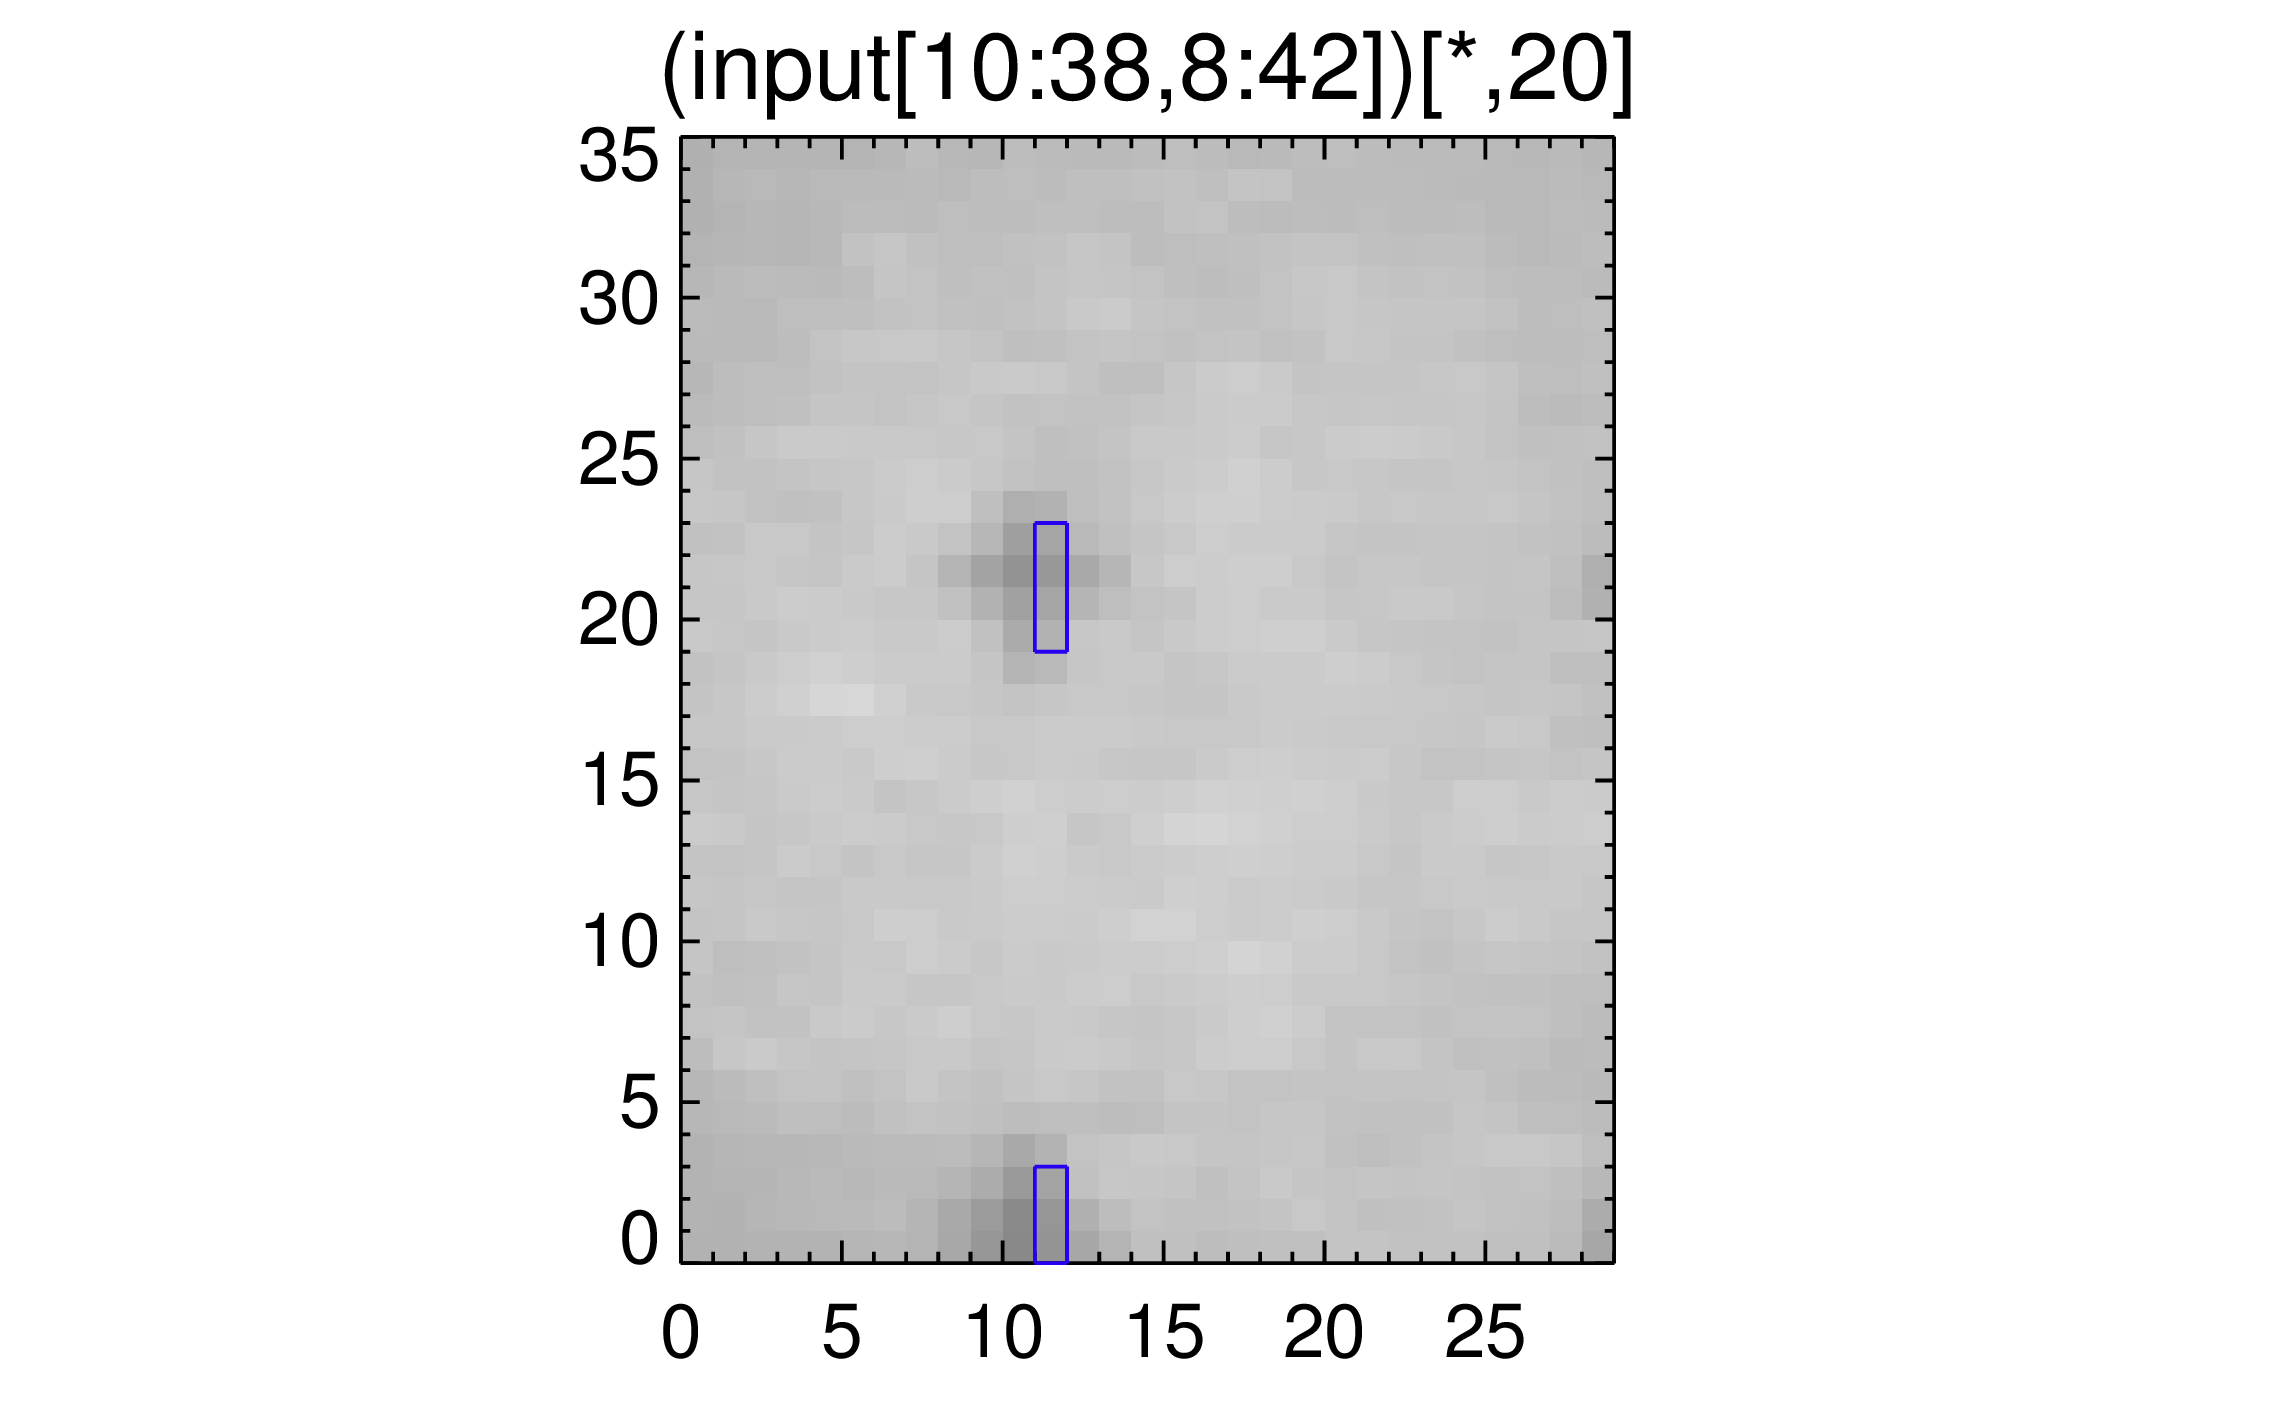
\includegraphics[width=.5\textwidth]{../plots_tables_images/fidcheck_withbothtruncate0.png}%
       }%
       {%
       \caption{1 Fiducial pixel in image}%
       }%
        \ffigbox[\Xhsize]%
       {%
       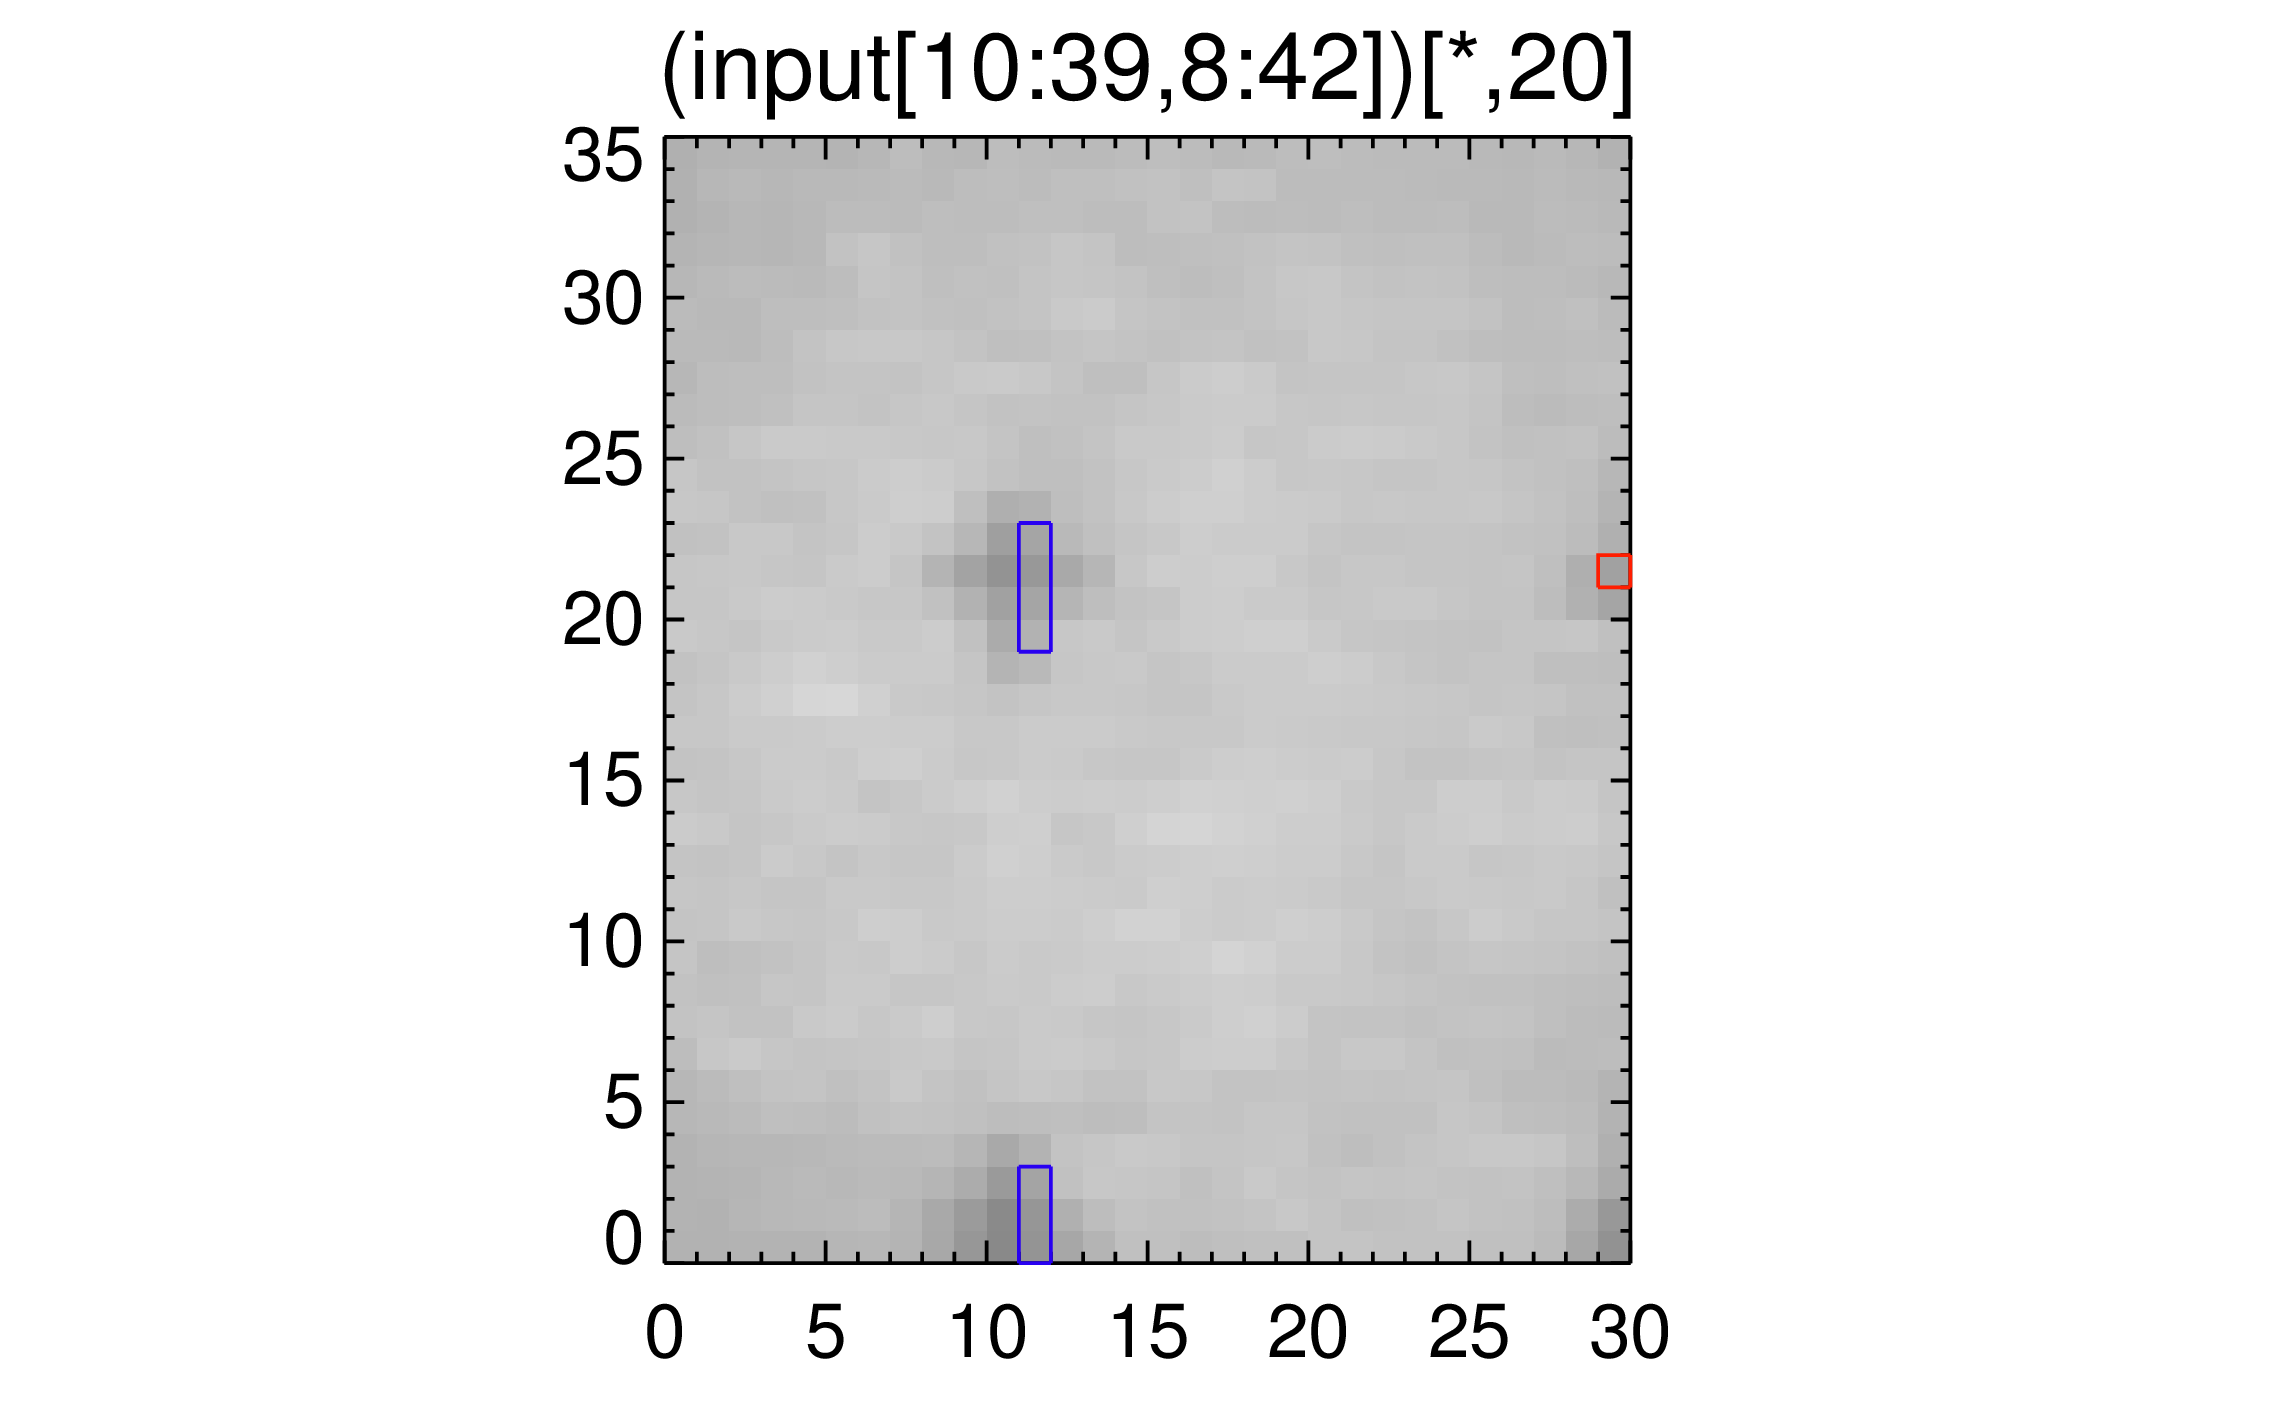
\includegraphics[width=.5\textwidth]{../plots_tables_images/fidcheck_withbothtruncate1.png}%
       }%
       {%
       \caption{2 pixels}%
       }%
    \end{subfloatrow}}

    \ffigbox[][\FBheight]{%
    \begin{subfloatrow}[2]%
        \ffigbox[\FBwidth]%
       {%
       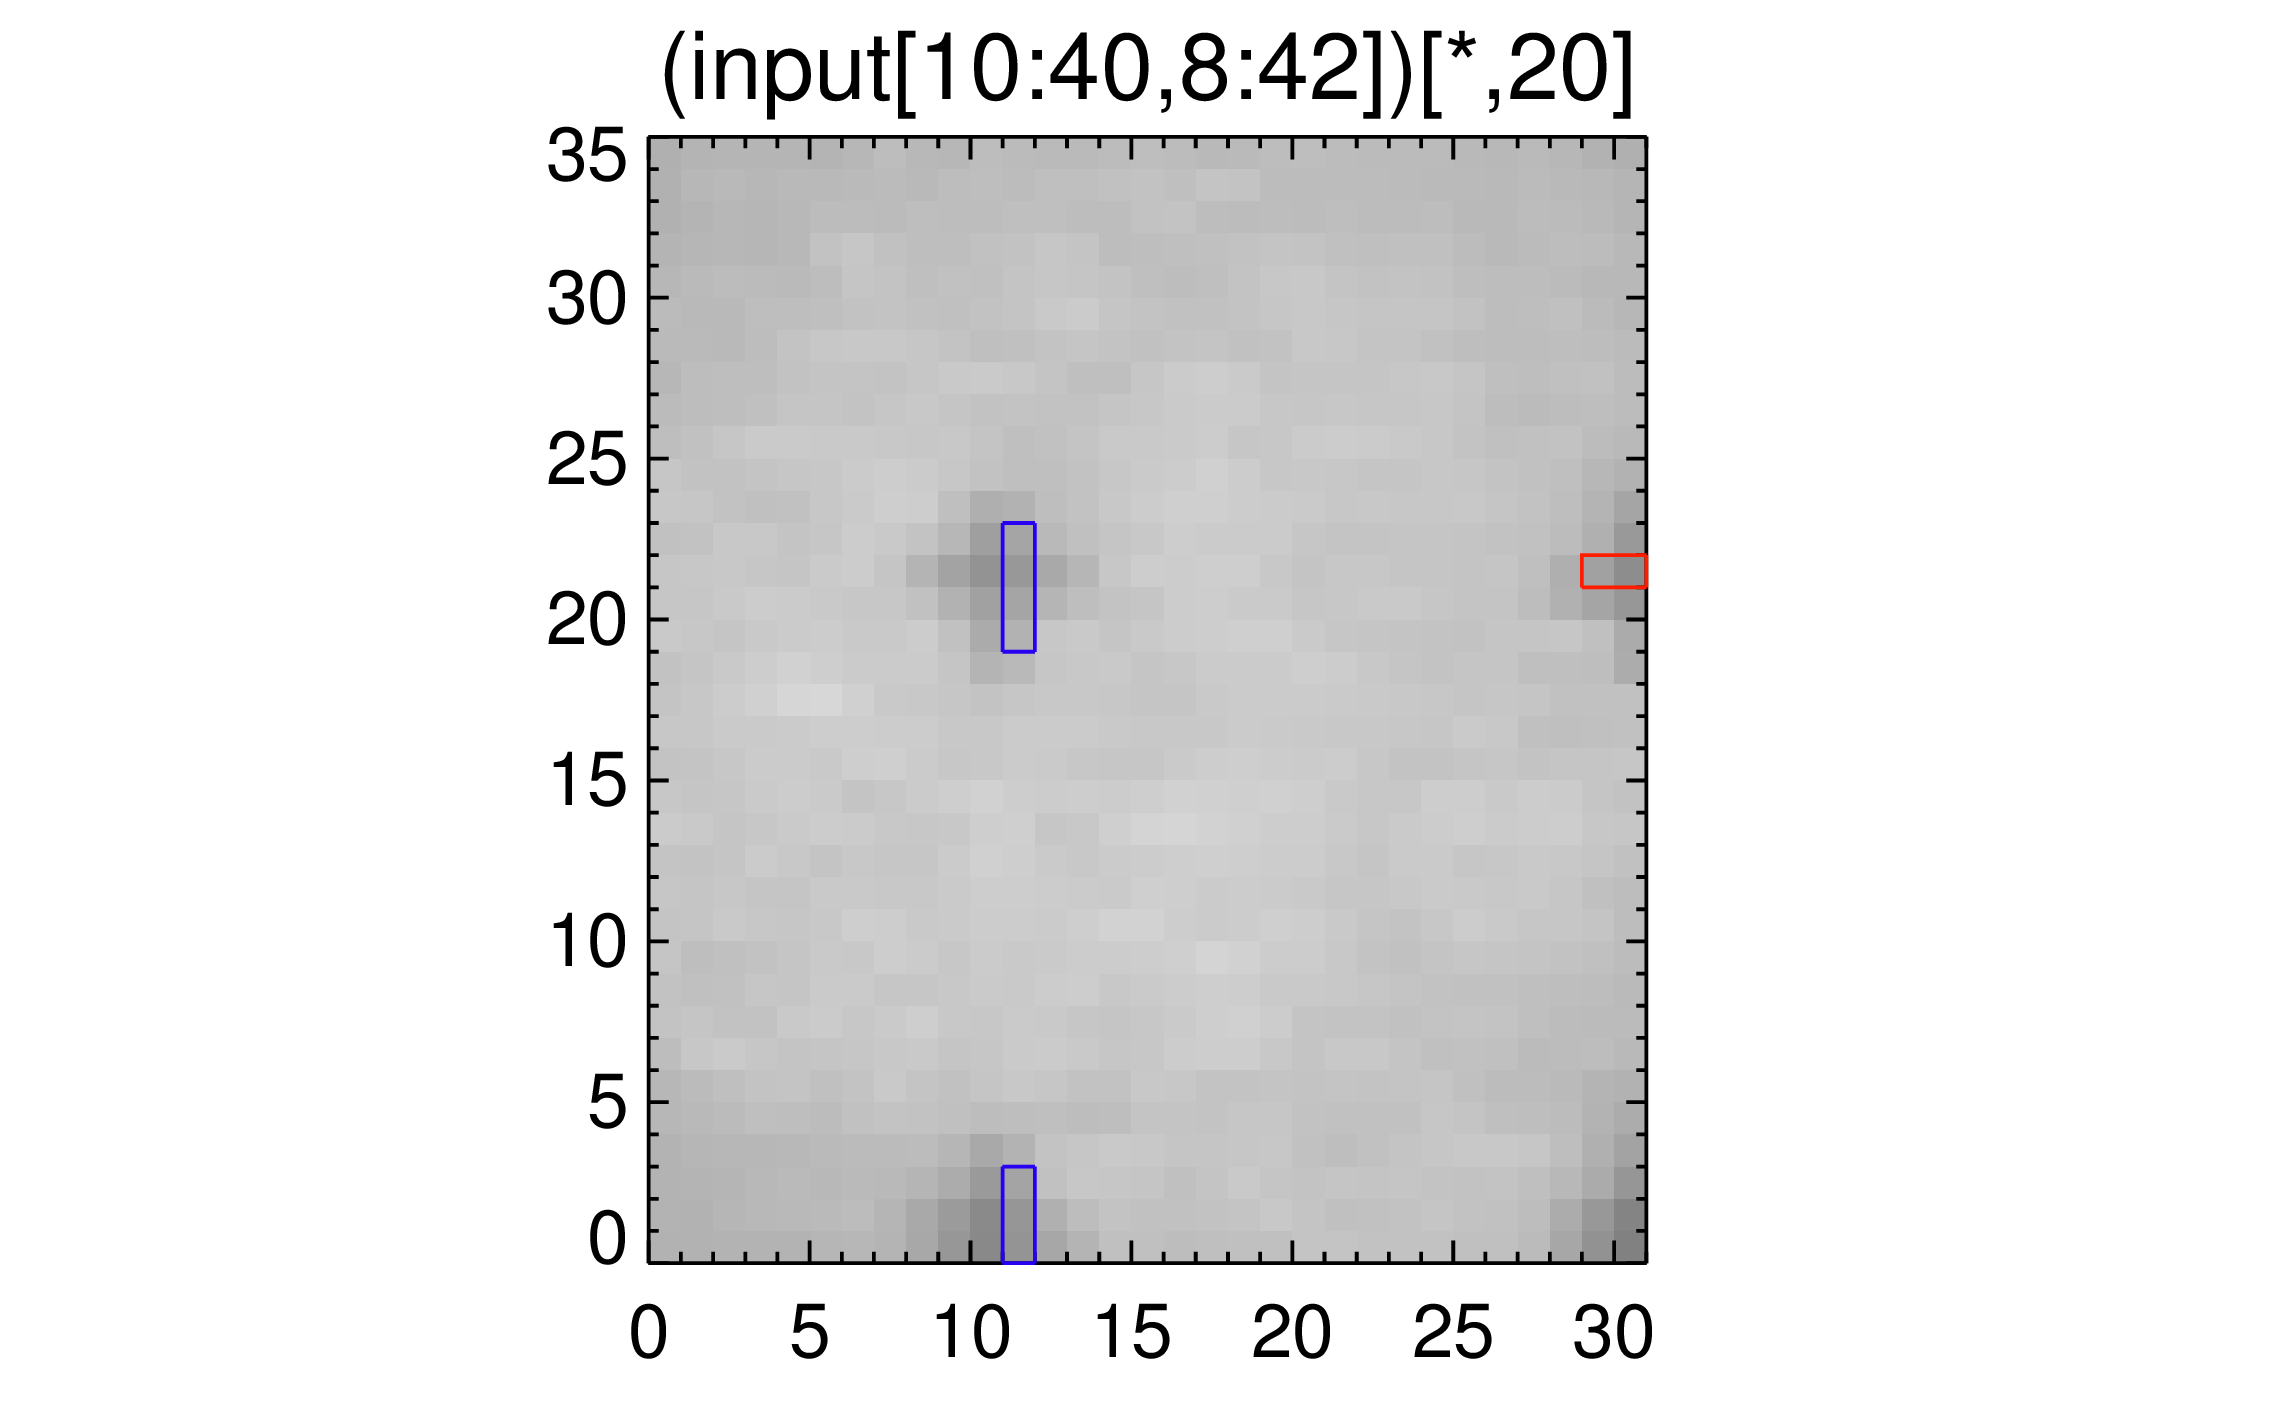
\includegraphics[width=.5\textwidth]{../plots_tables_images/fidcheck_withbothtruncate2.png}%
       }%
       {%
       \caption{3 pixels}%
       }%
        \ffigbox[\Xhsize]%
       {%
       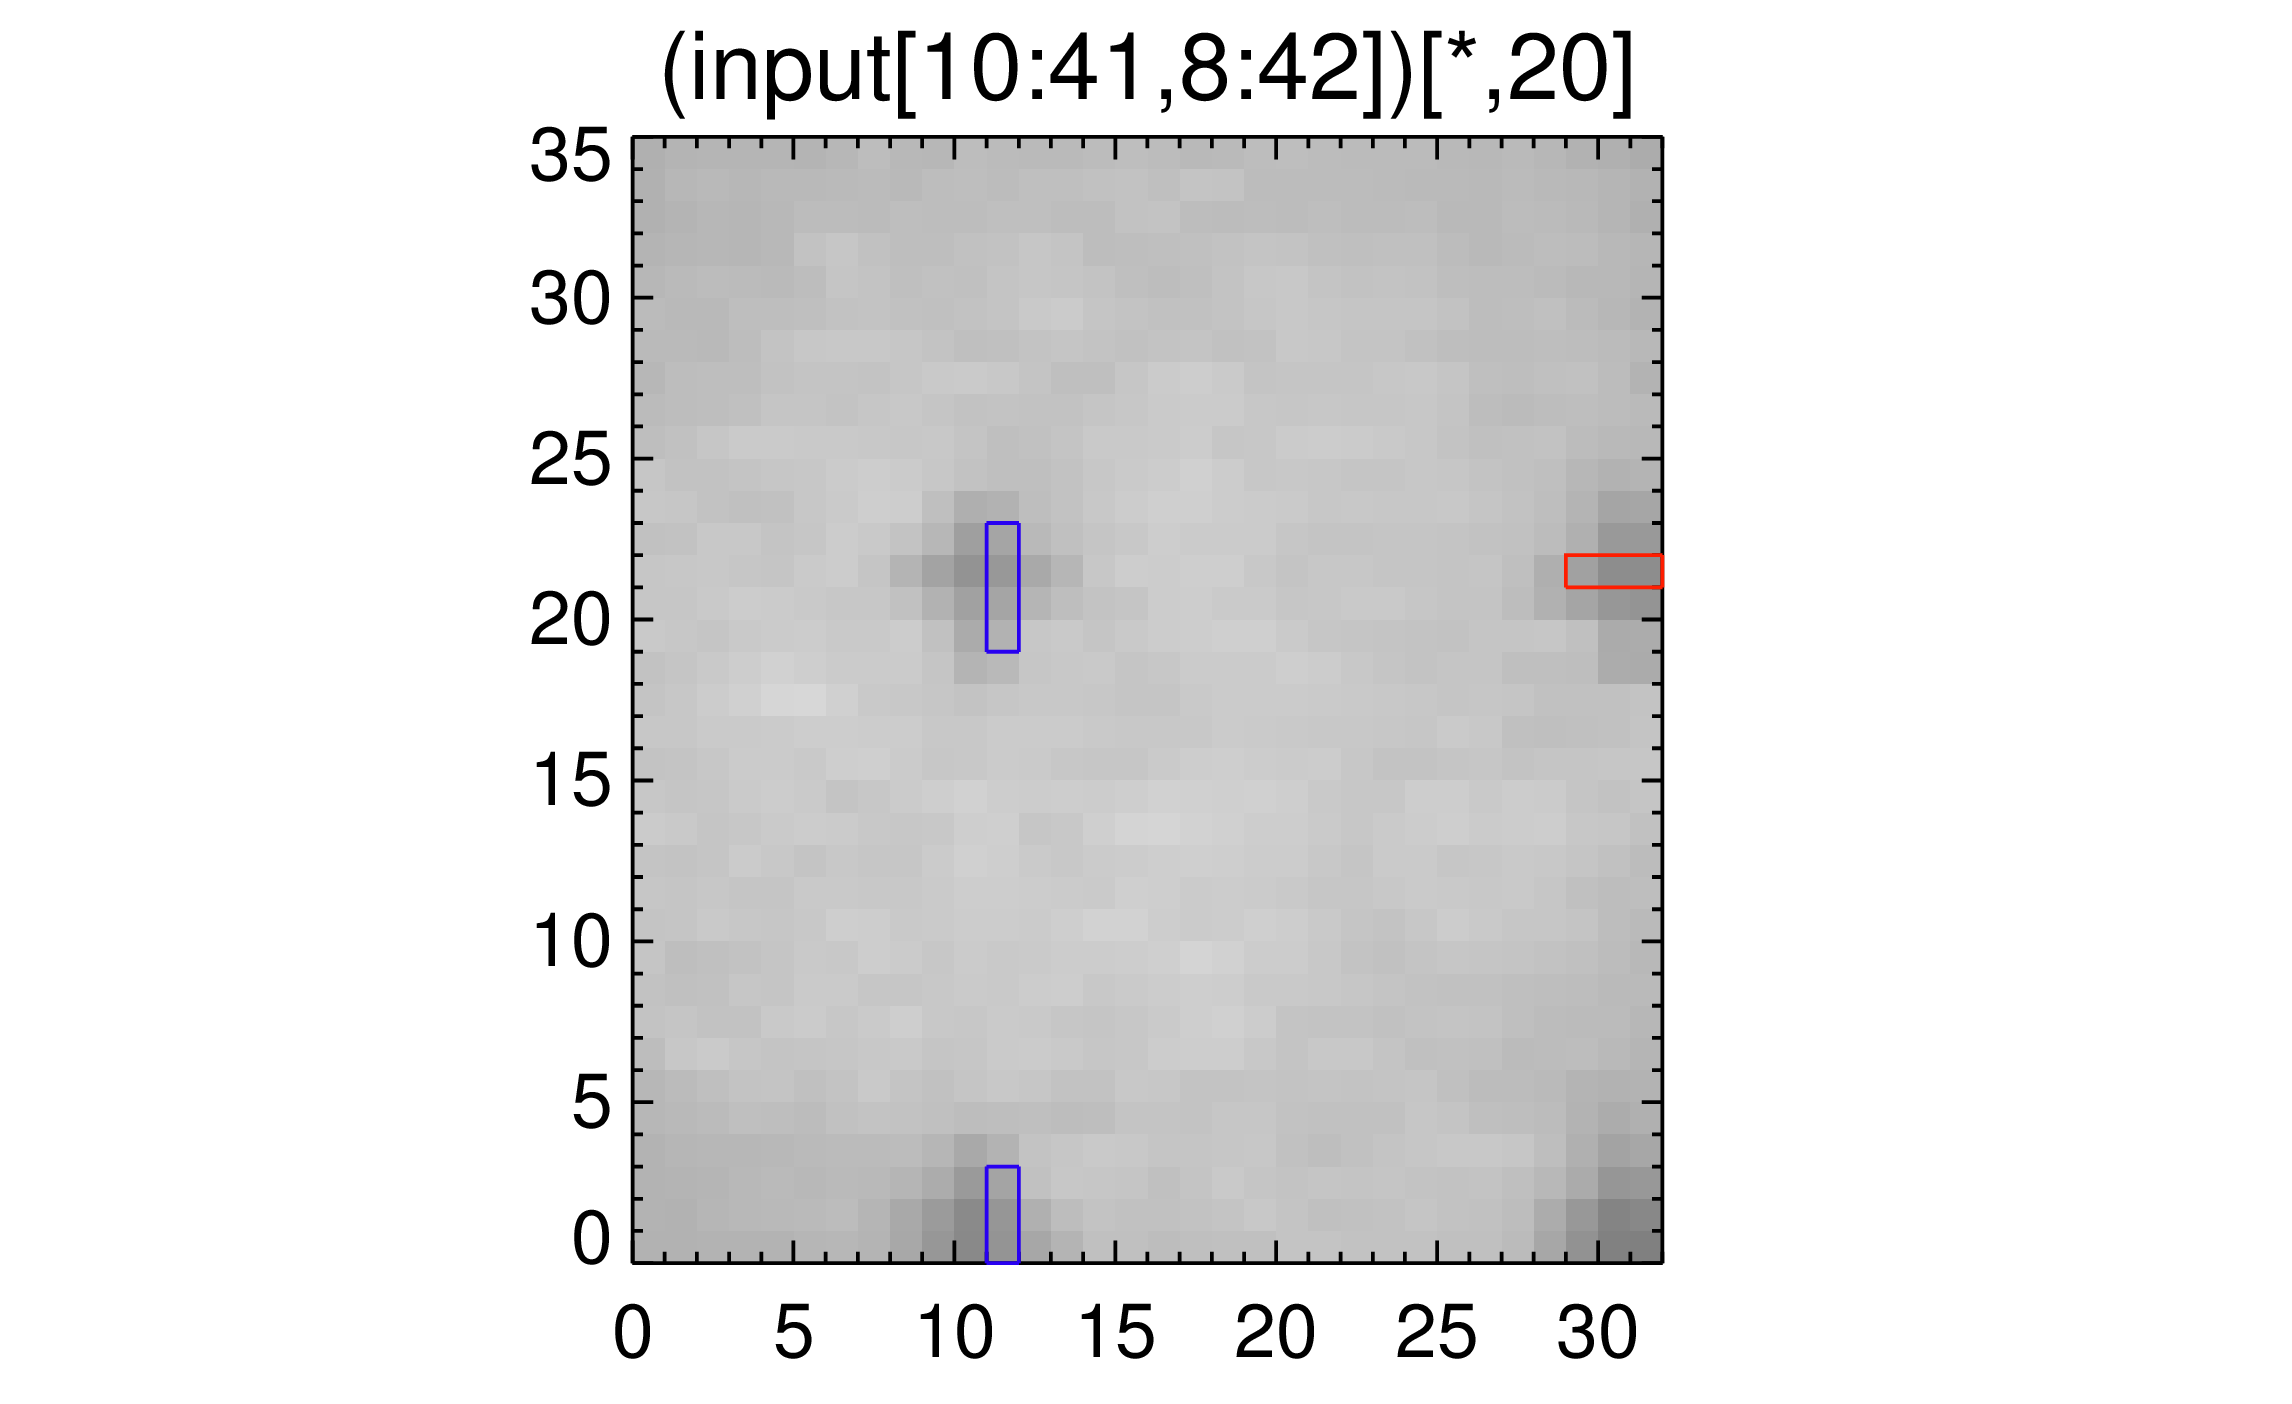
\includegraphics[width=.5\textwidth]{../plots_tables_images/fidcheck_withbothtruncate3.png}%
       }%
       {%
       \caption{4 pixels}%
       }%
    \end{subfloatrow}}

        \ffigbox[][\FBheight]{%
    \begin{subfloatrow}[2]%
        \ffigbox[\FBwidth]%
       {%
       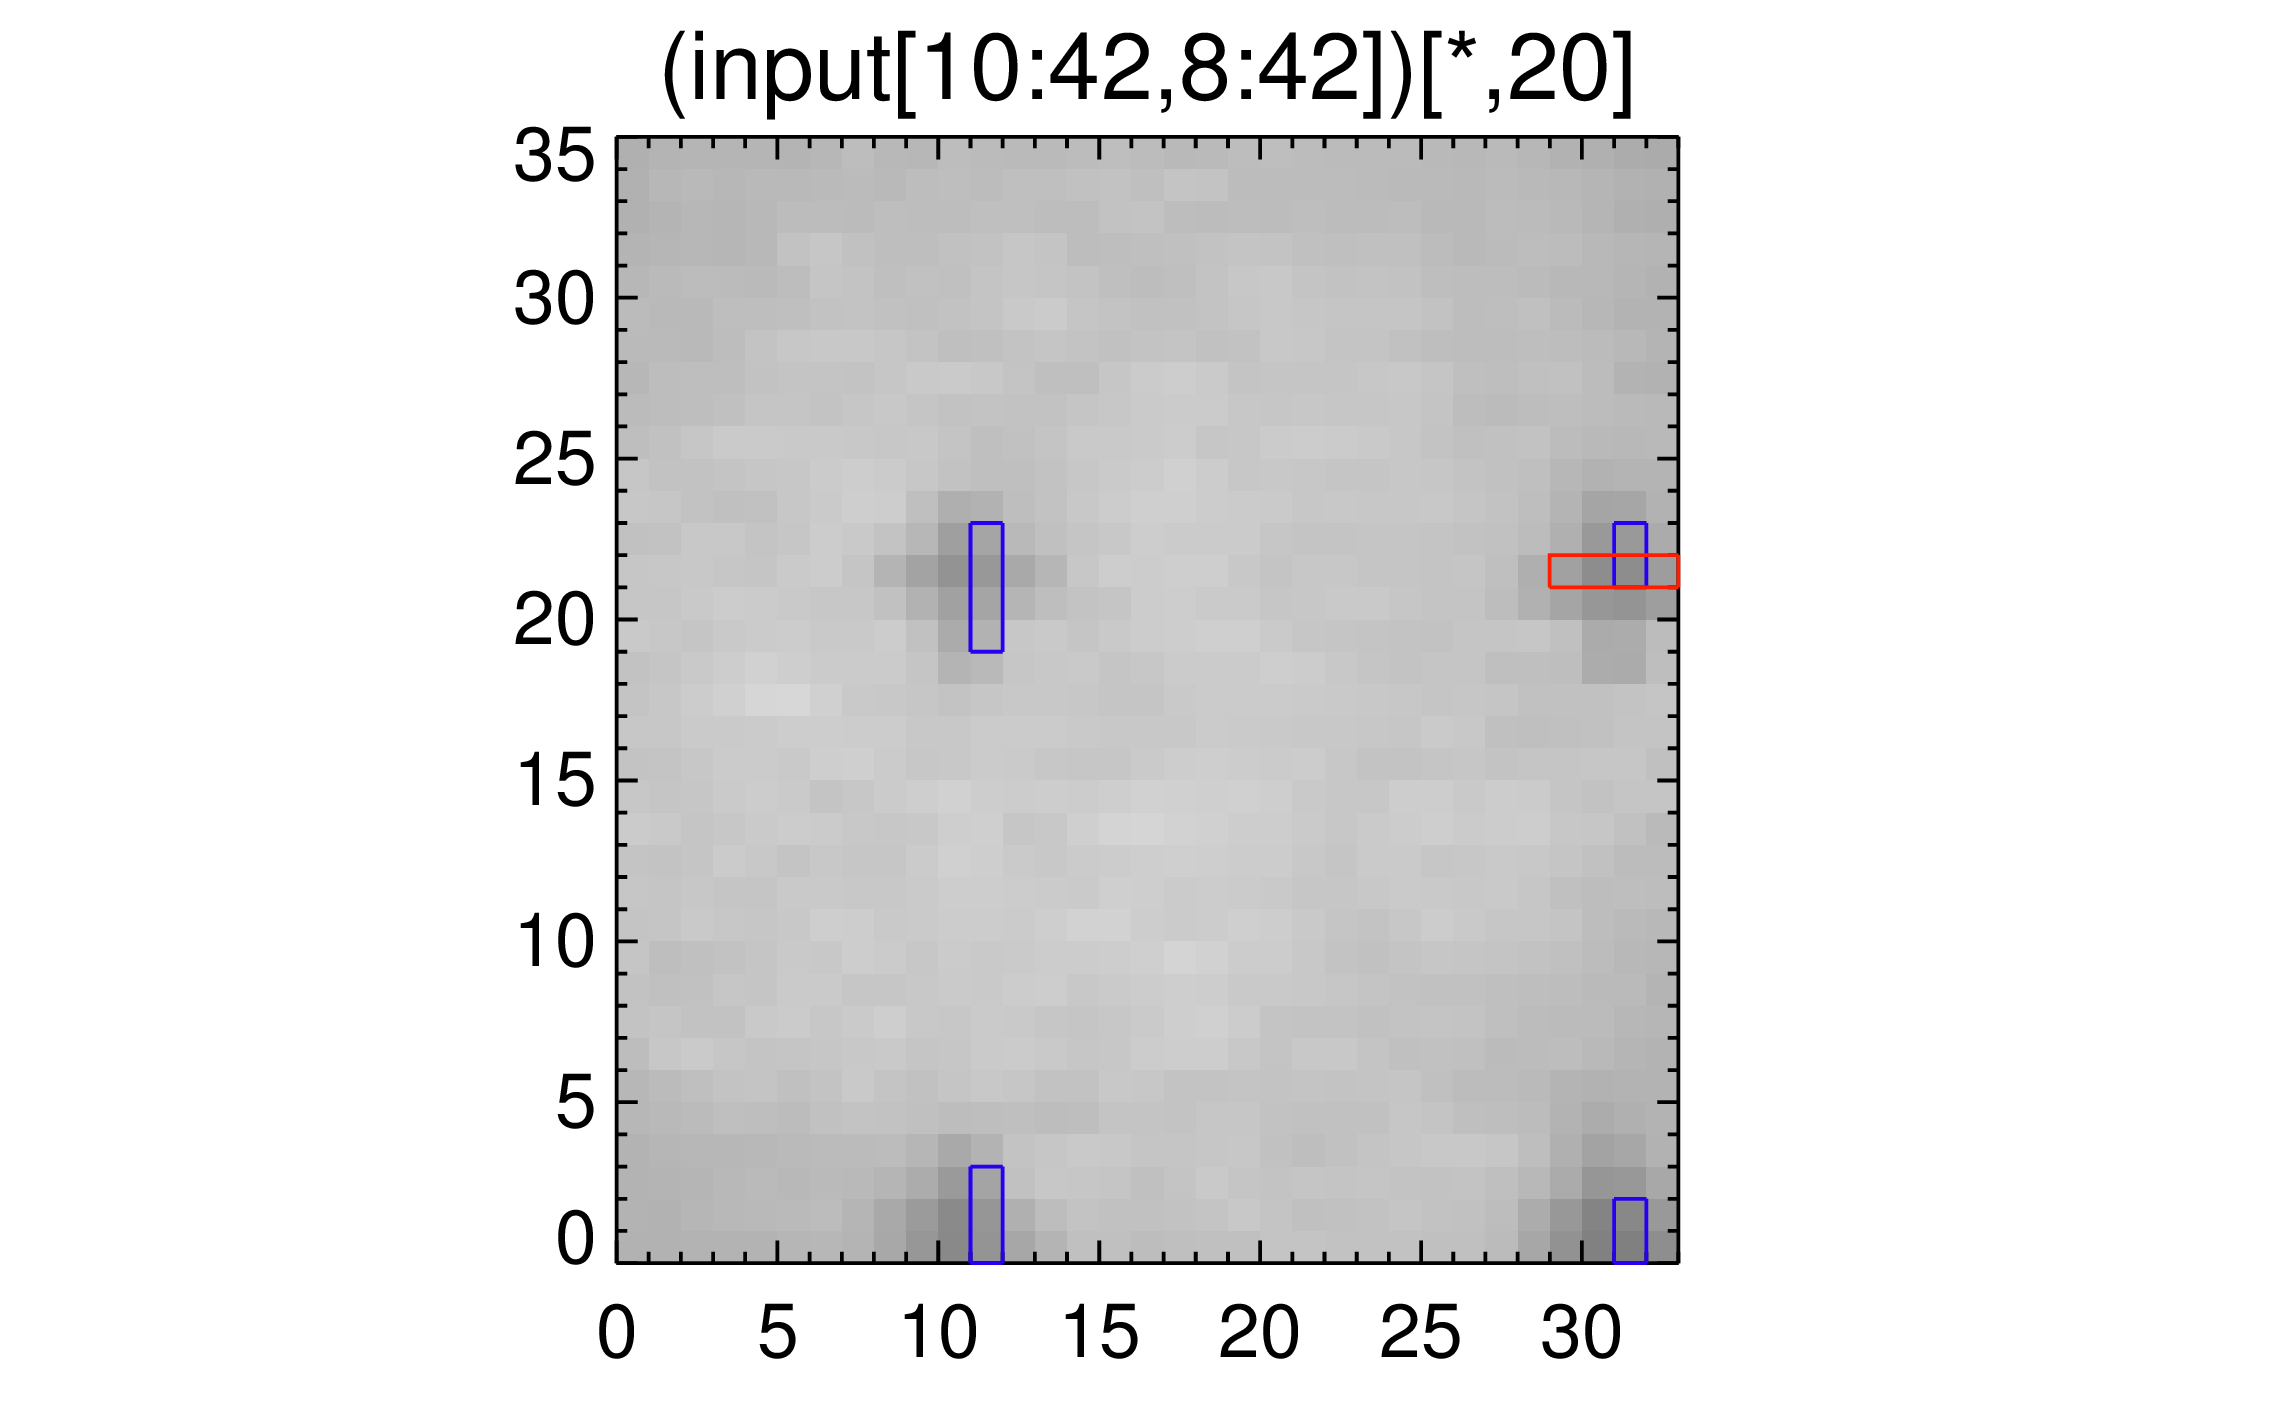
\includegraphics[width=.5\textwidth]{../plots_tables_images/fidcheck_withbothtruncate4.png}%
       }%
       {%
       \caption{5 pixels}%
       }%
        \ffigbox[\Xhsize]%
       {%
       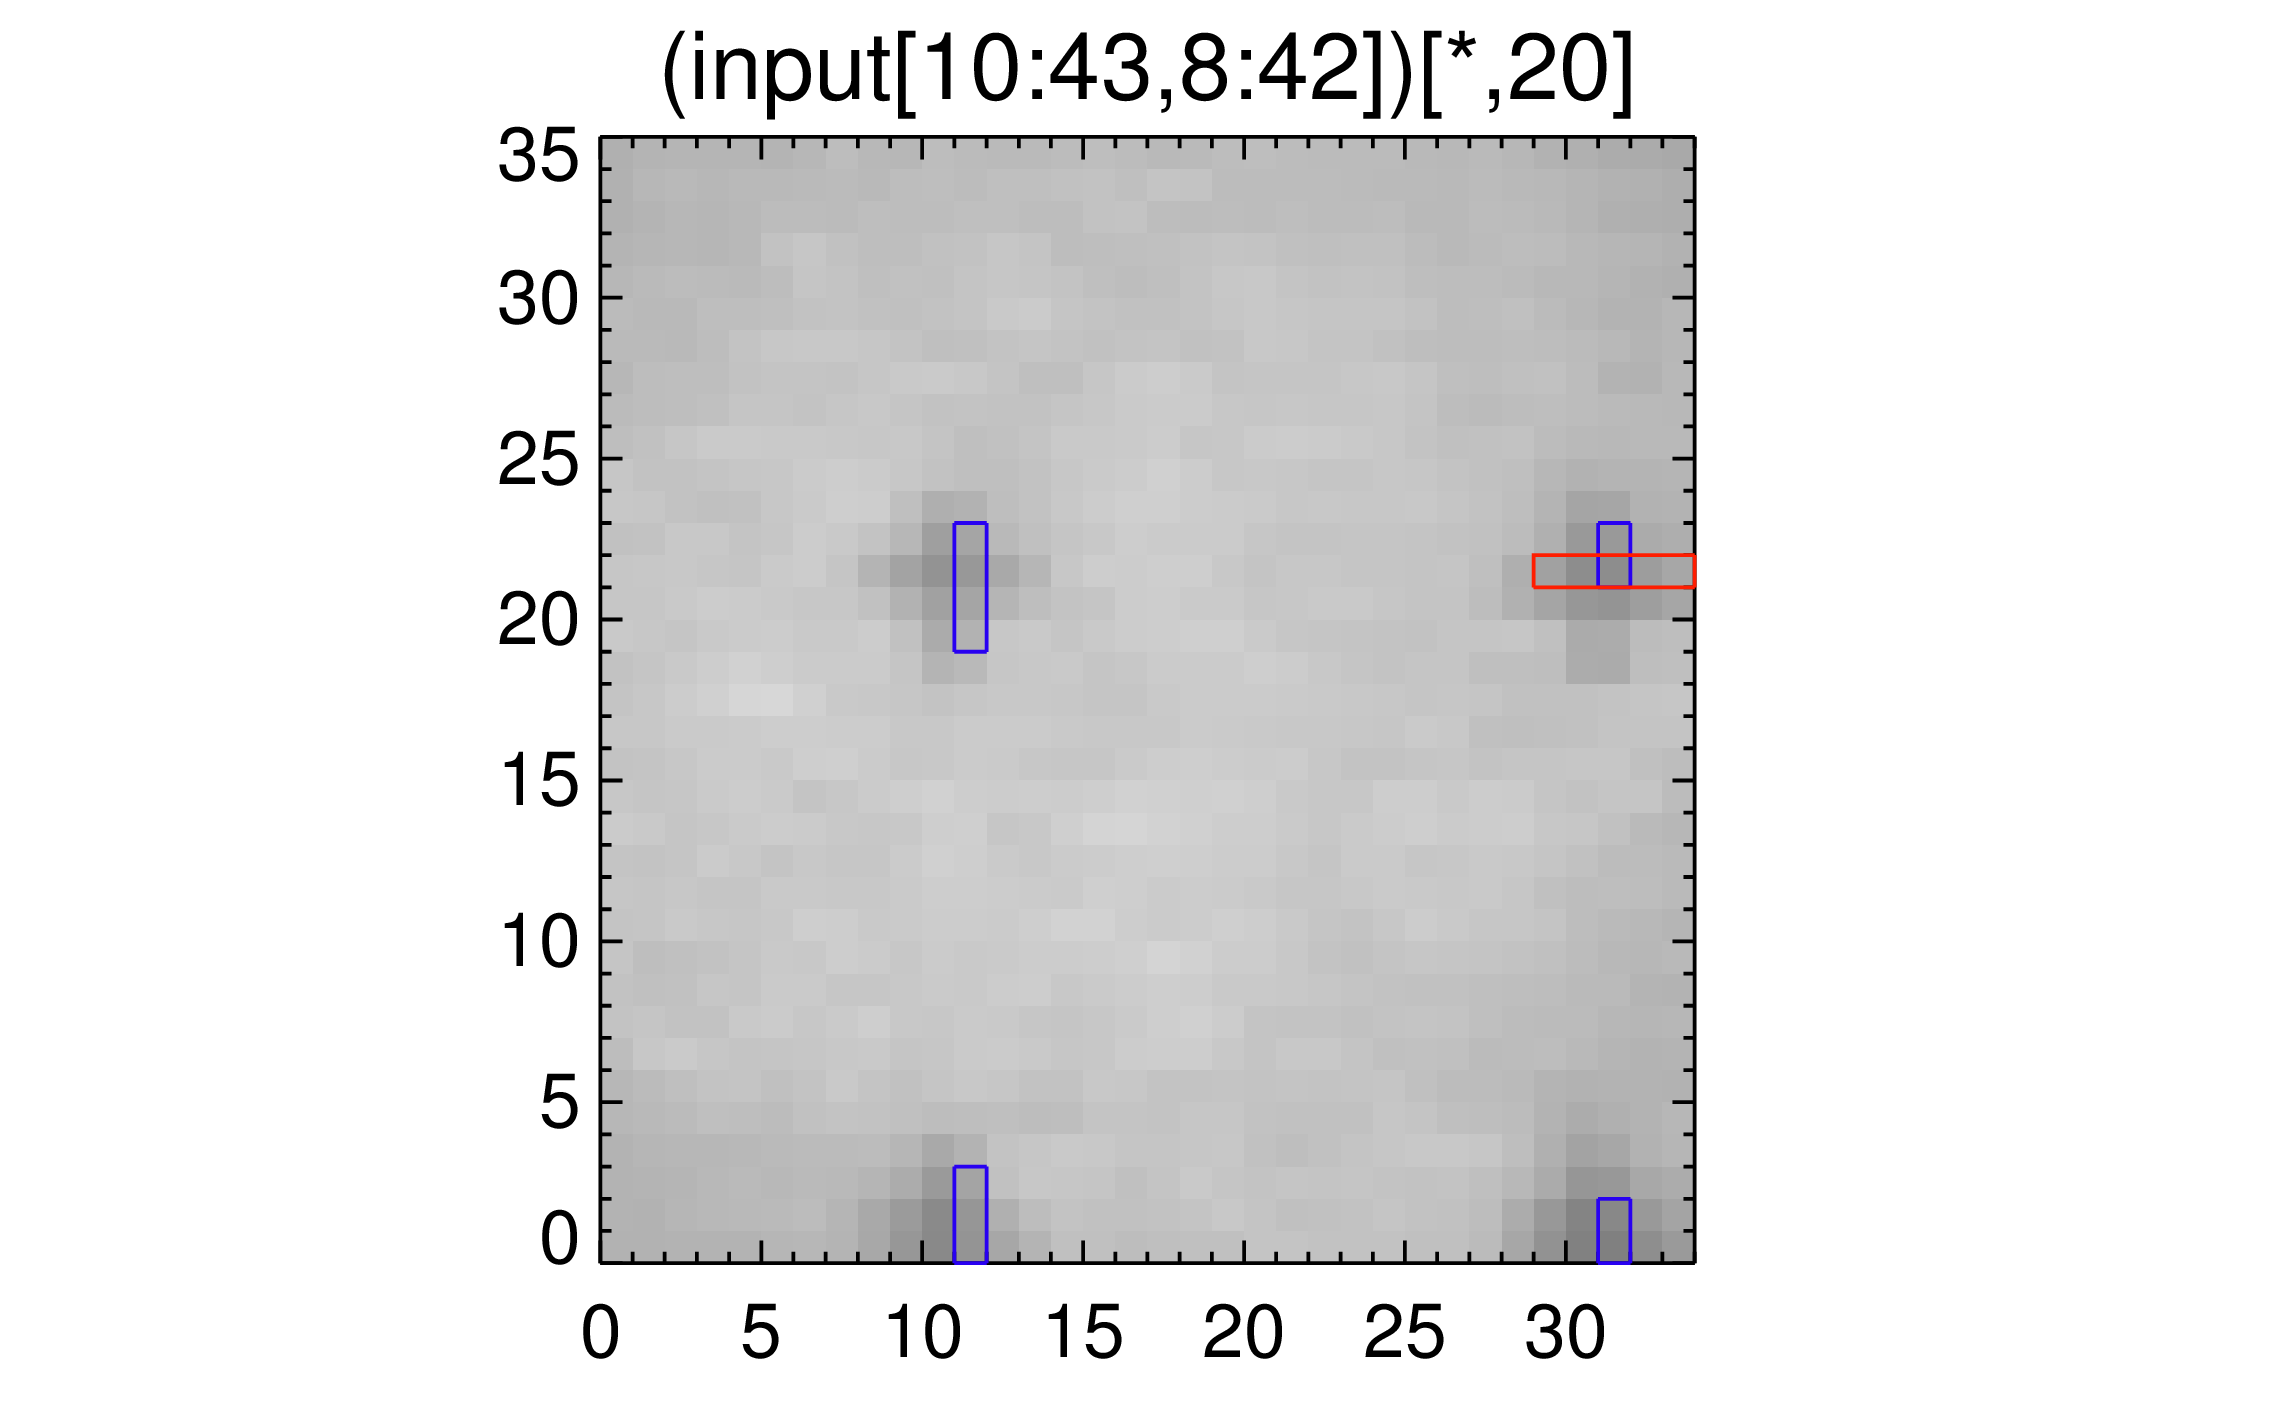
\includegraphics[width=.5\textwidth]{../plots_tables_images/fidcheck_withbothtruncate5.png}%
       }%
       {%
       \caption{Completely in image}%
       }%
    \end{subfloatrow}}{\caption{Result of \hl{\texttt{shift\_diff(emboss(image,/edge\_truncate),/edge\_truncate)}}. The top left is the most cropped image and the bottom right is the least cropped image.}\label{first_plot}}%
\end{figure}

% \begin{figure}[!h]
%     \centering 
%     \begin{subfigure}[b]{.45\linewidth}
%         \centering
%         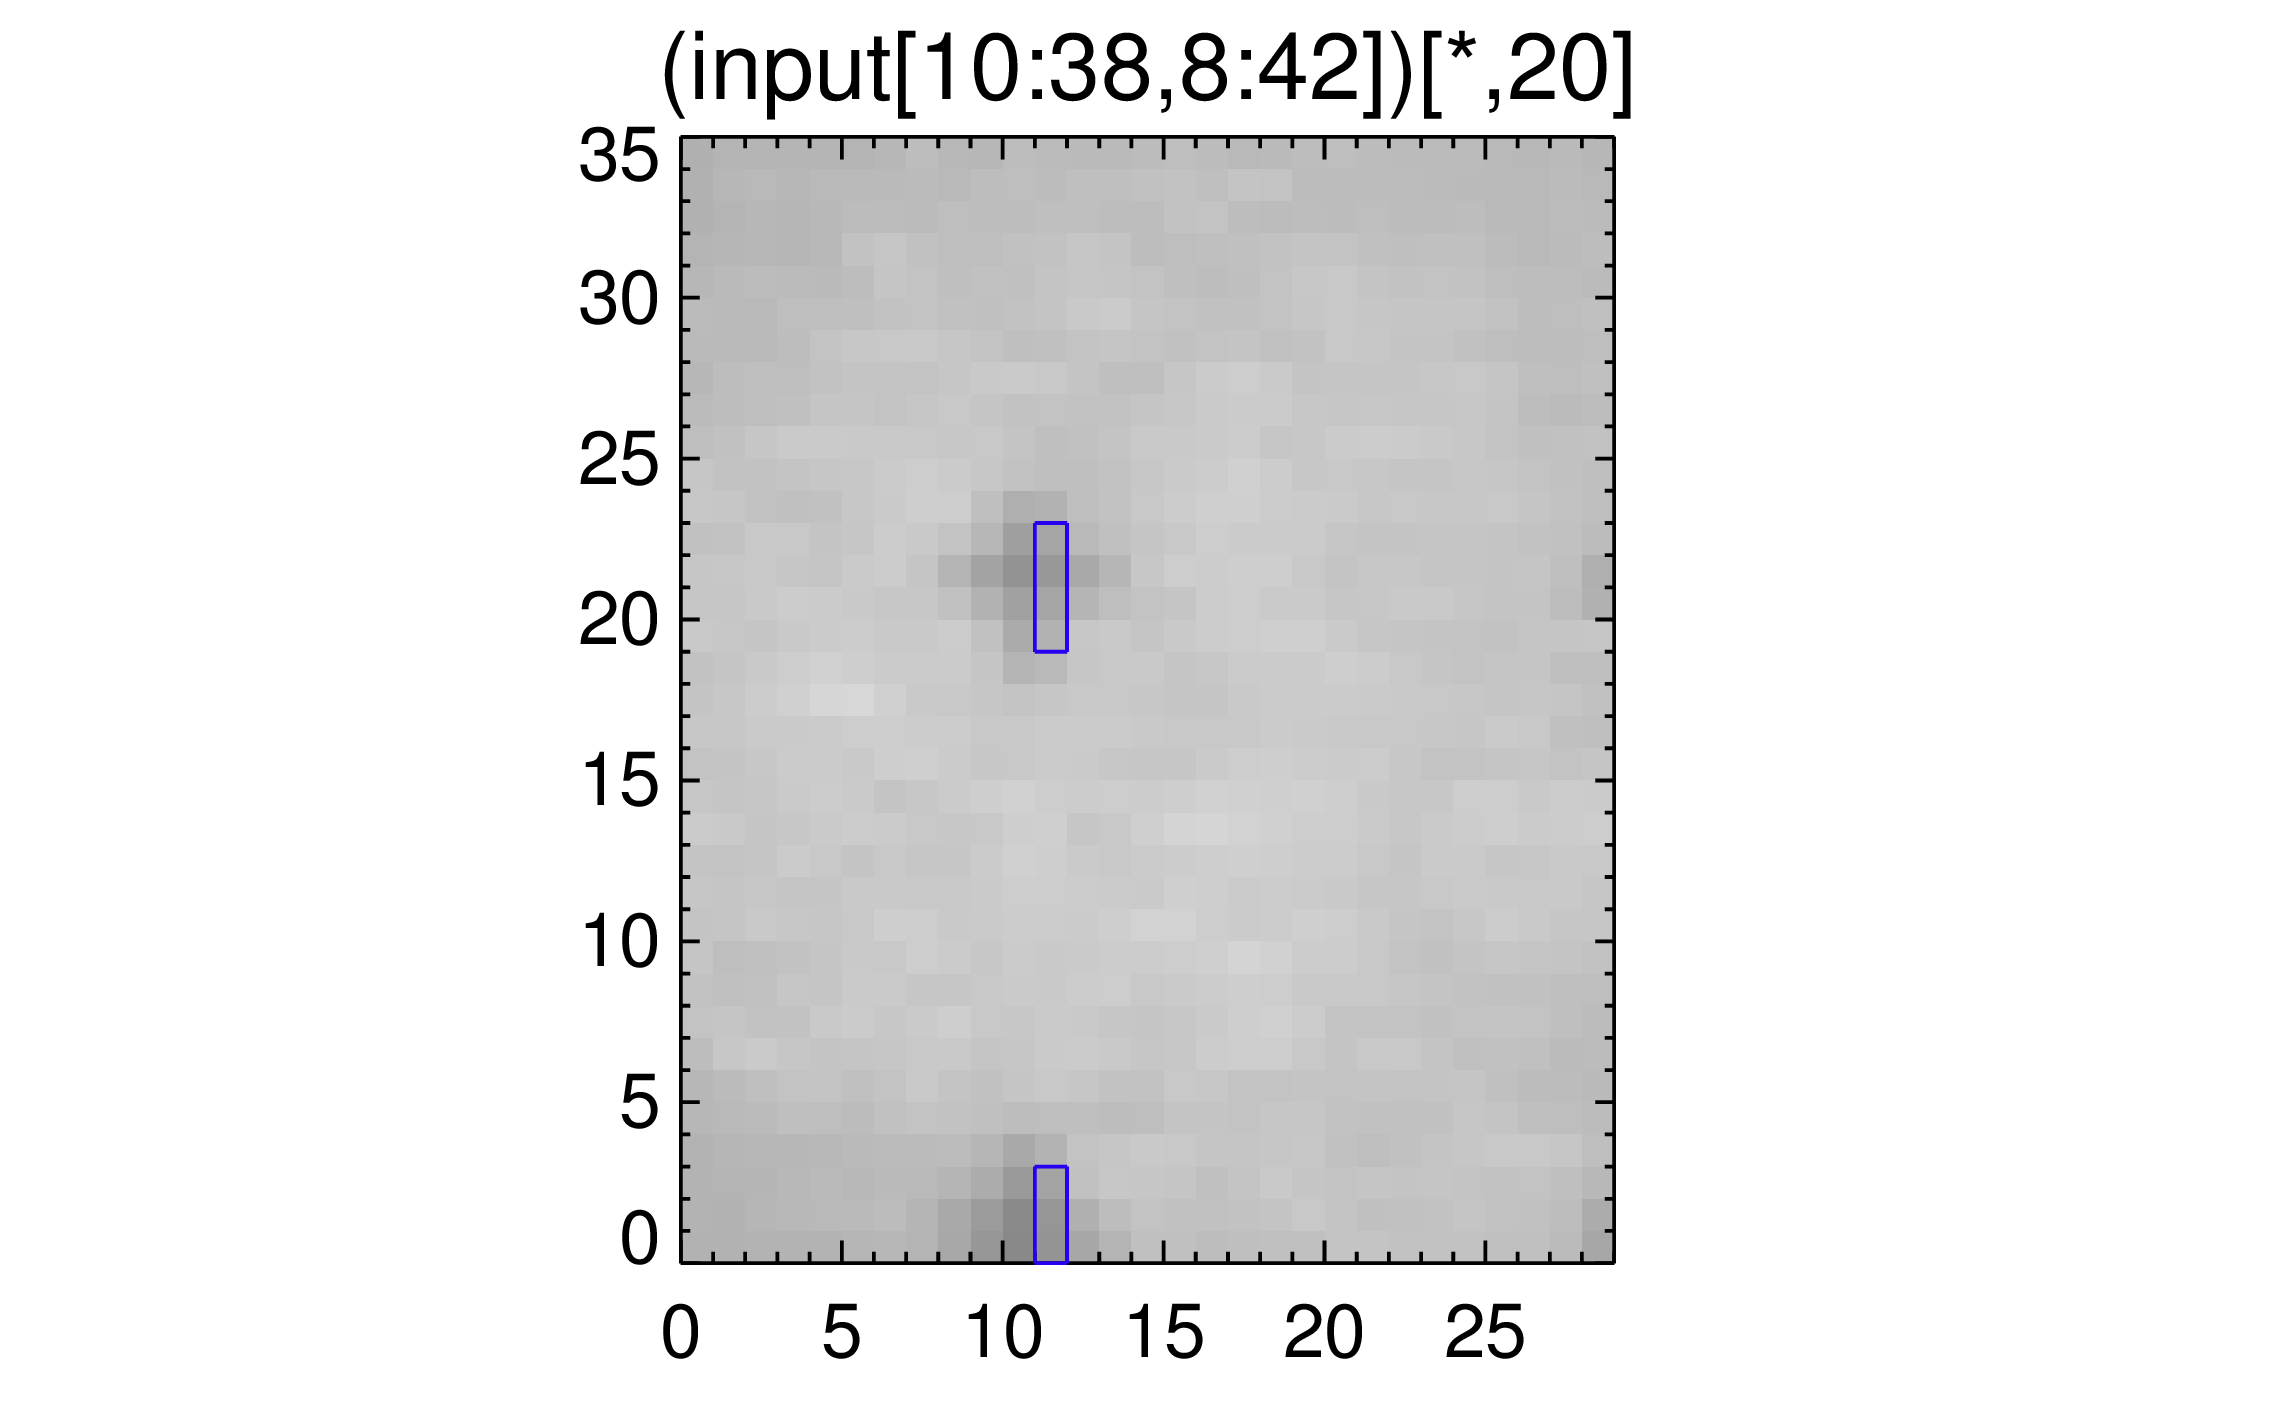
\includegraphics[width=1.3\textwidth]{../plots_tables_images/fidcheck_withbothtruncate0.png}
%         \caption{1 Fiducial pixel in image}
%     \end{subfigure}
%     \begin{subfigure}[b]{.45\linewidth}
%         \centering
%         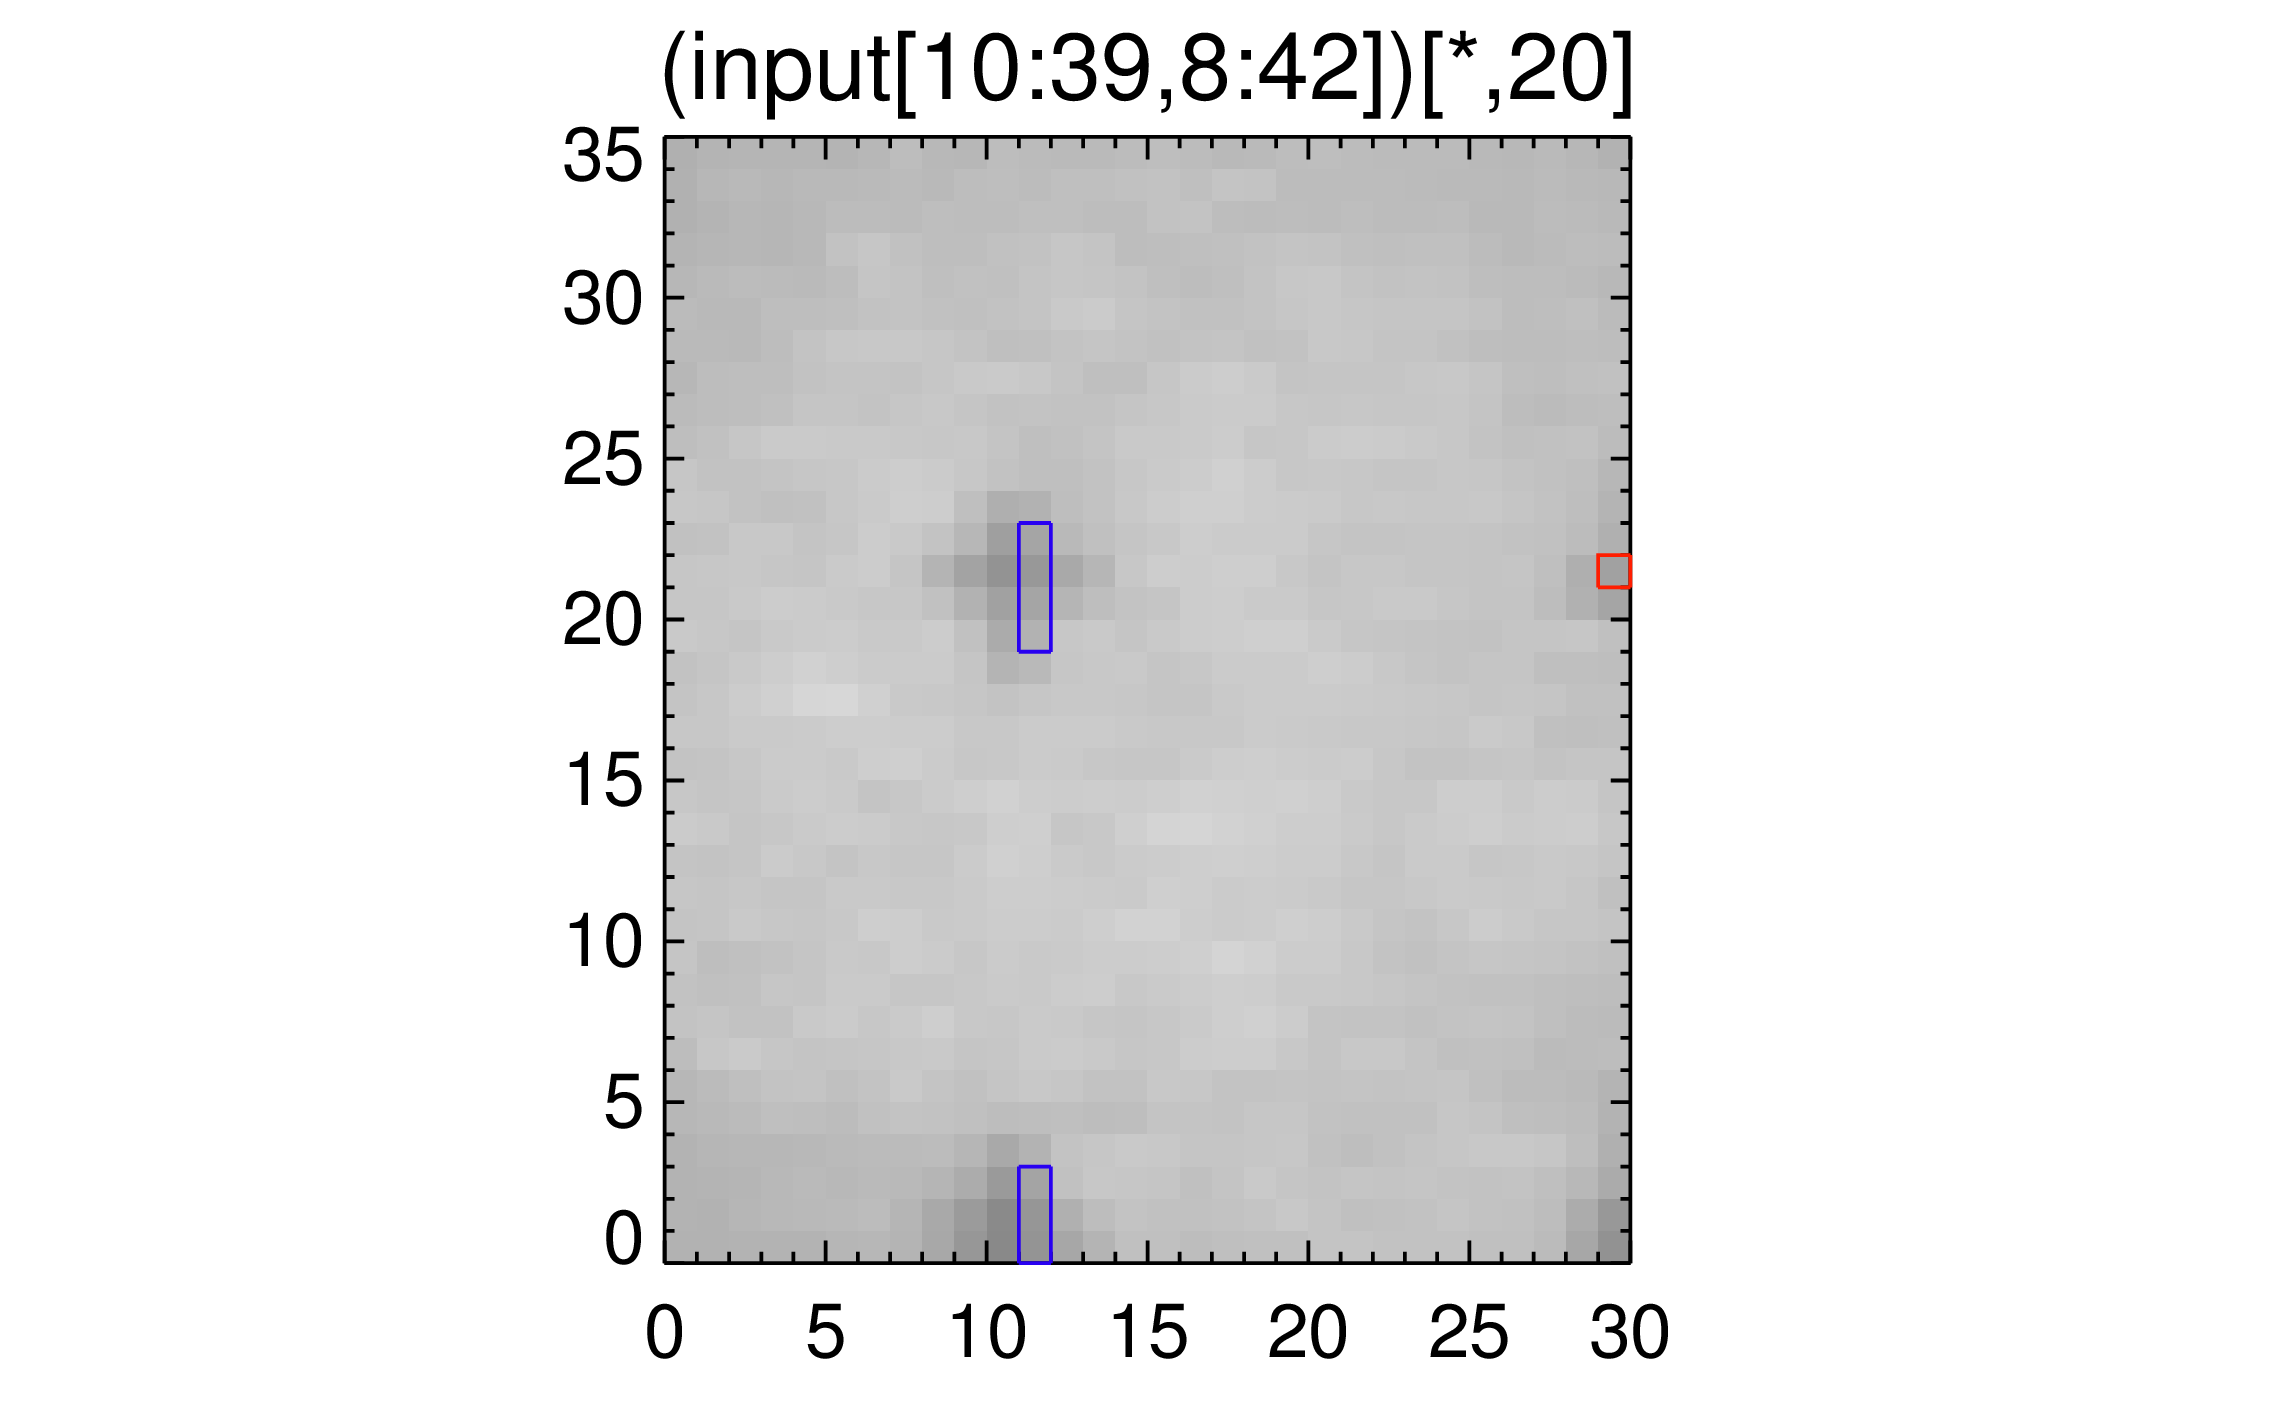
\includegraphics[width=1.3\textwidth]{../plots_tables_images/fidcheck_withbothtruncate1.png}
%         \caption{2 pixels}
%     \end{subfigure}
   
%    \begin{subfigure}[b]{.45\linewidth}
%         \centering
%         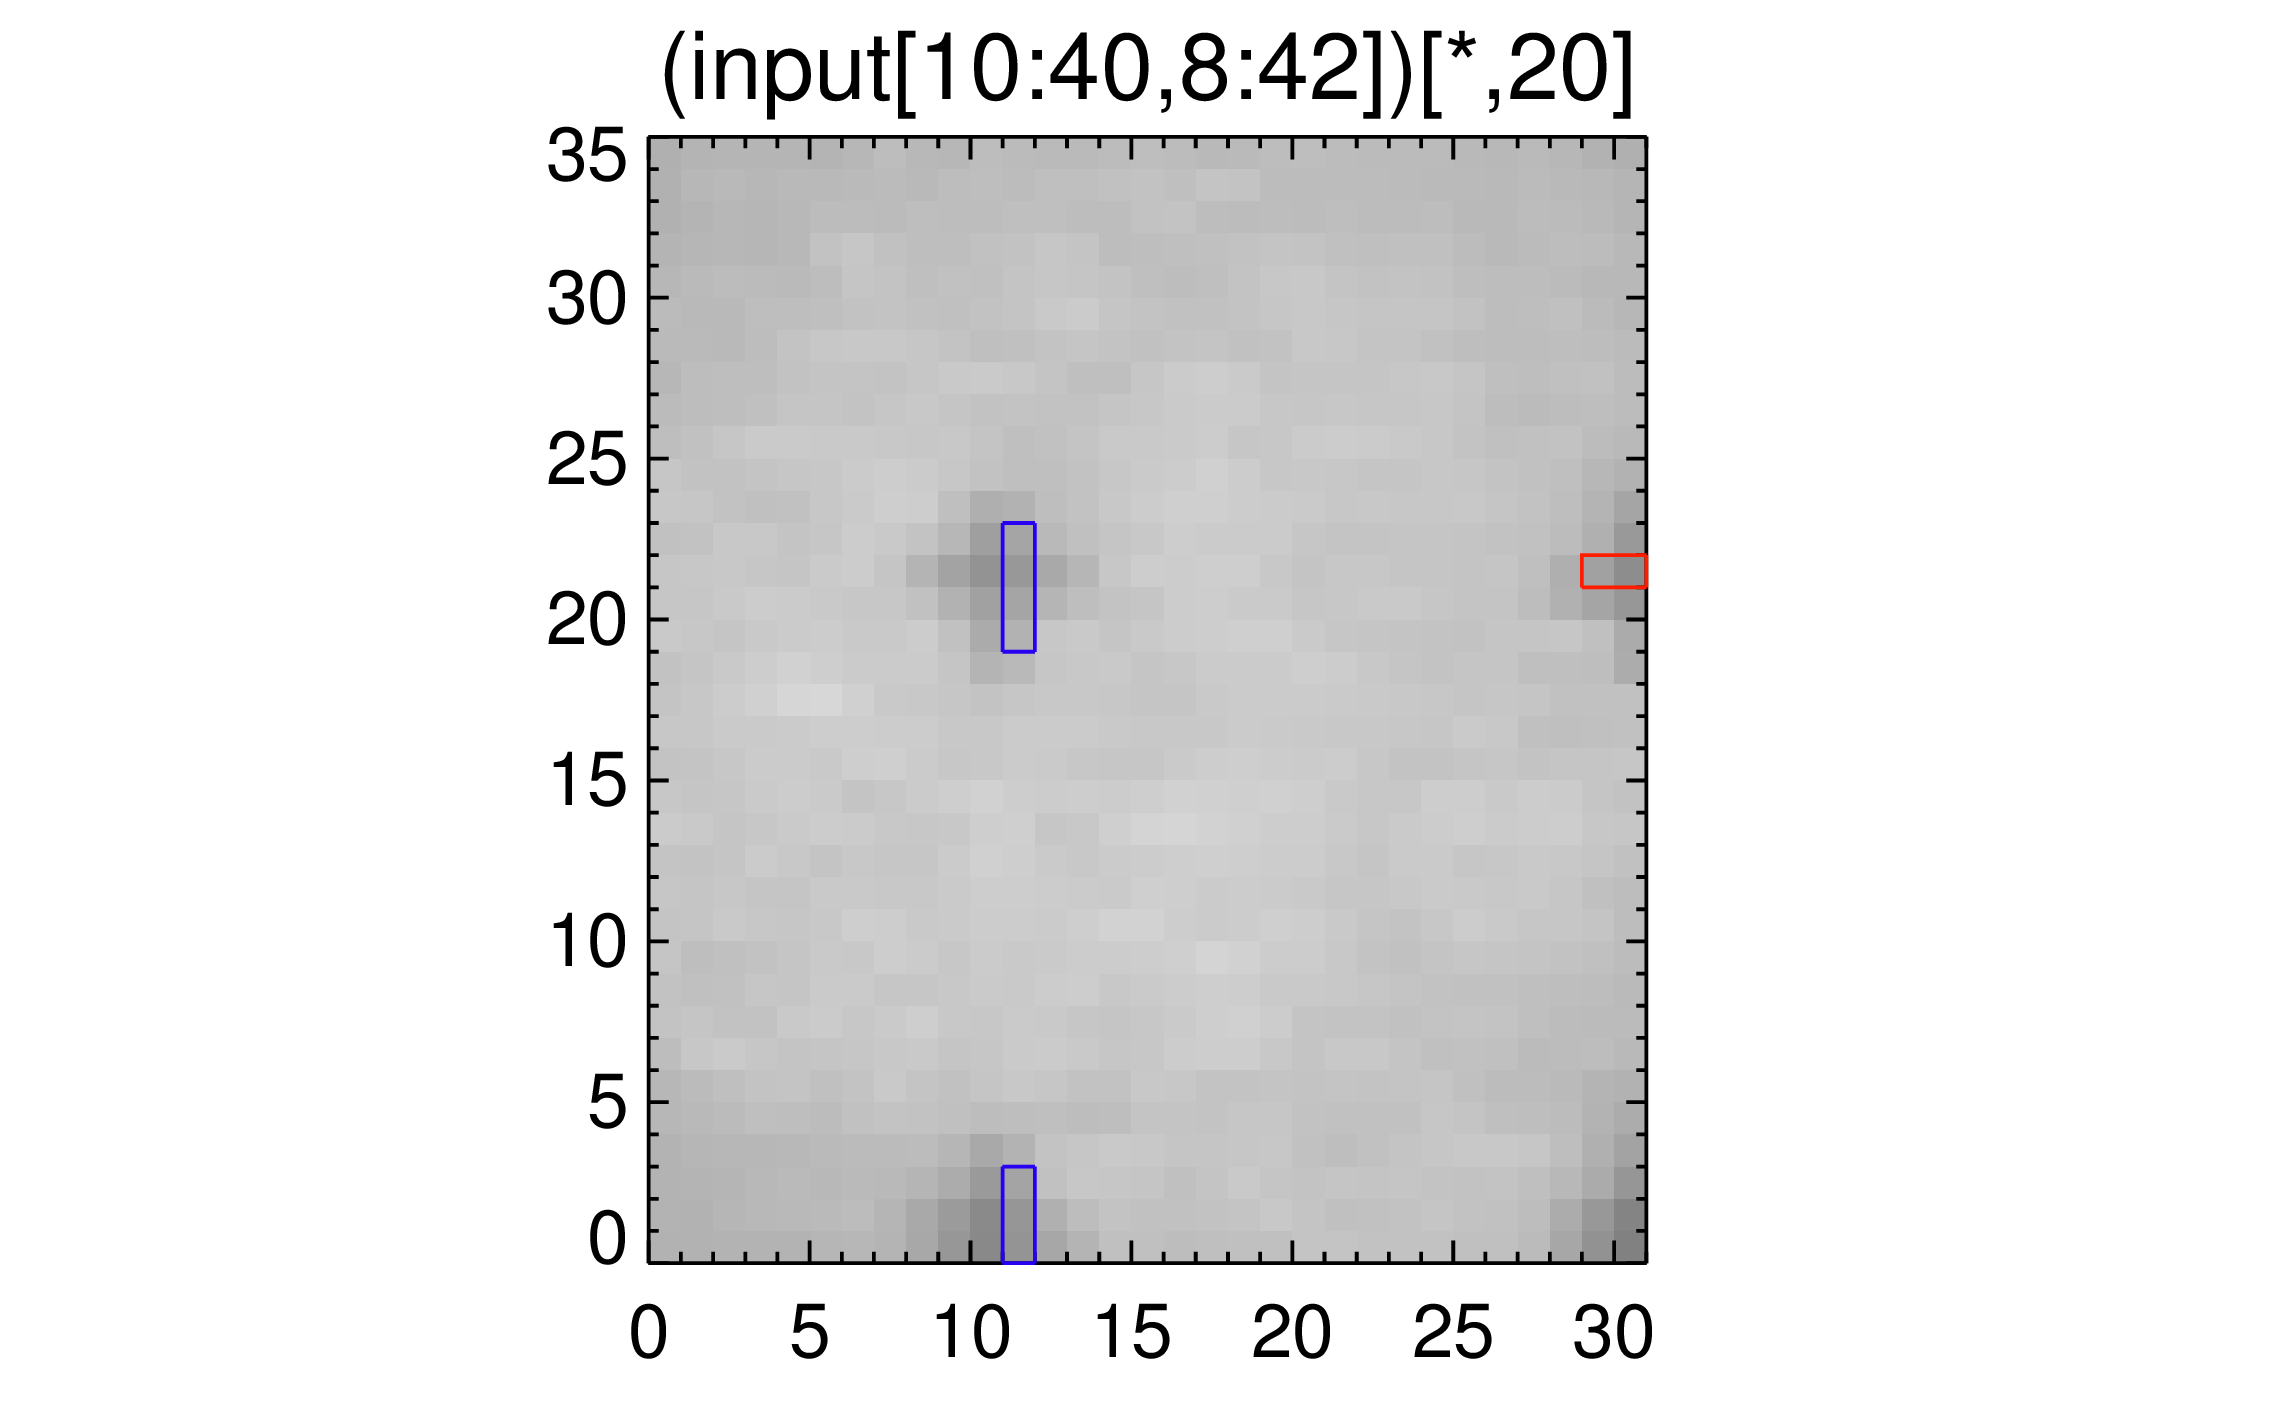
\includegraphics[width=1.3\textwidth]{../plots_tables_images/fidcheck_withbothtruncate2.png}
%         \caption{3 pixels}
%     \end{subfigure}
%     \begin{subfigure}[b]{.45\linewidth}
%         \centering
%         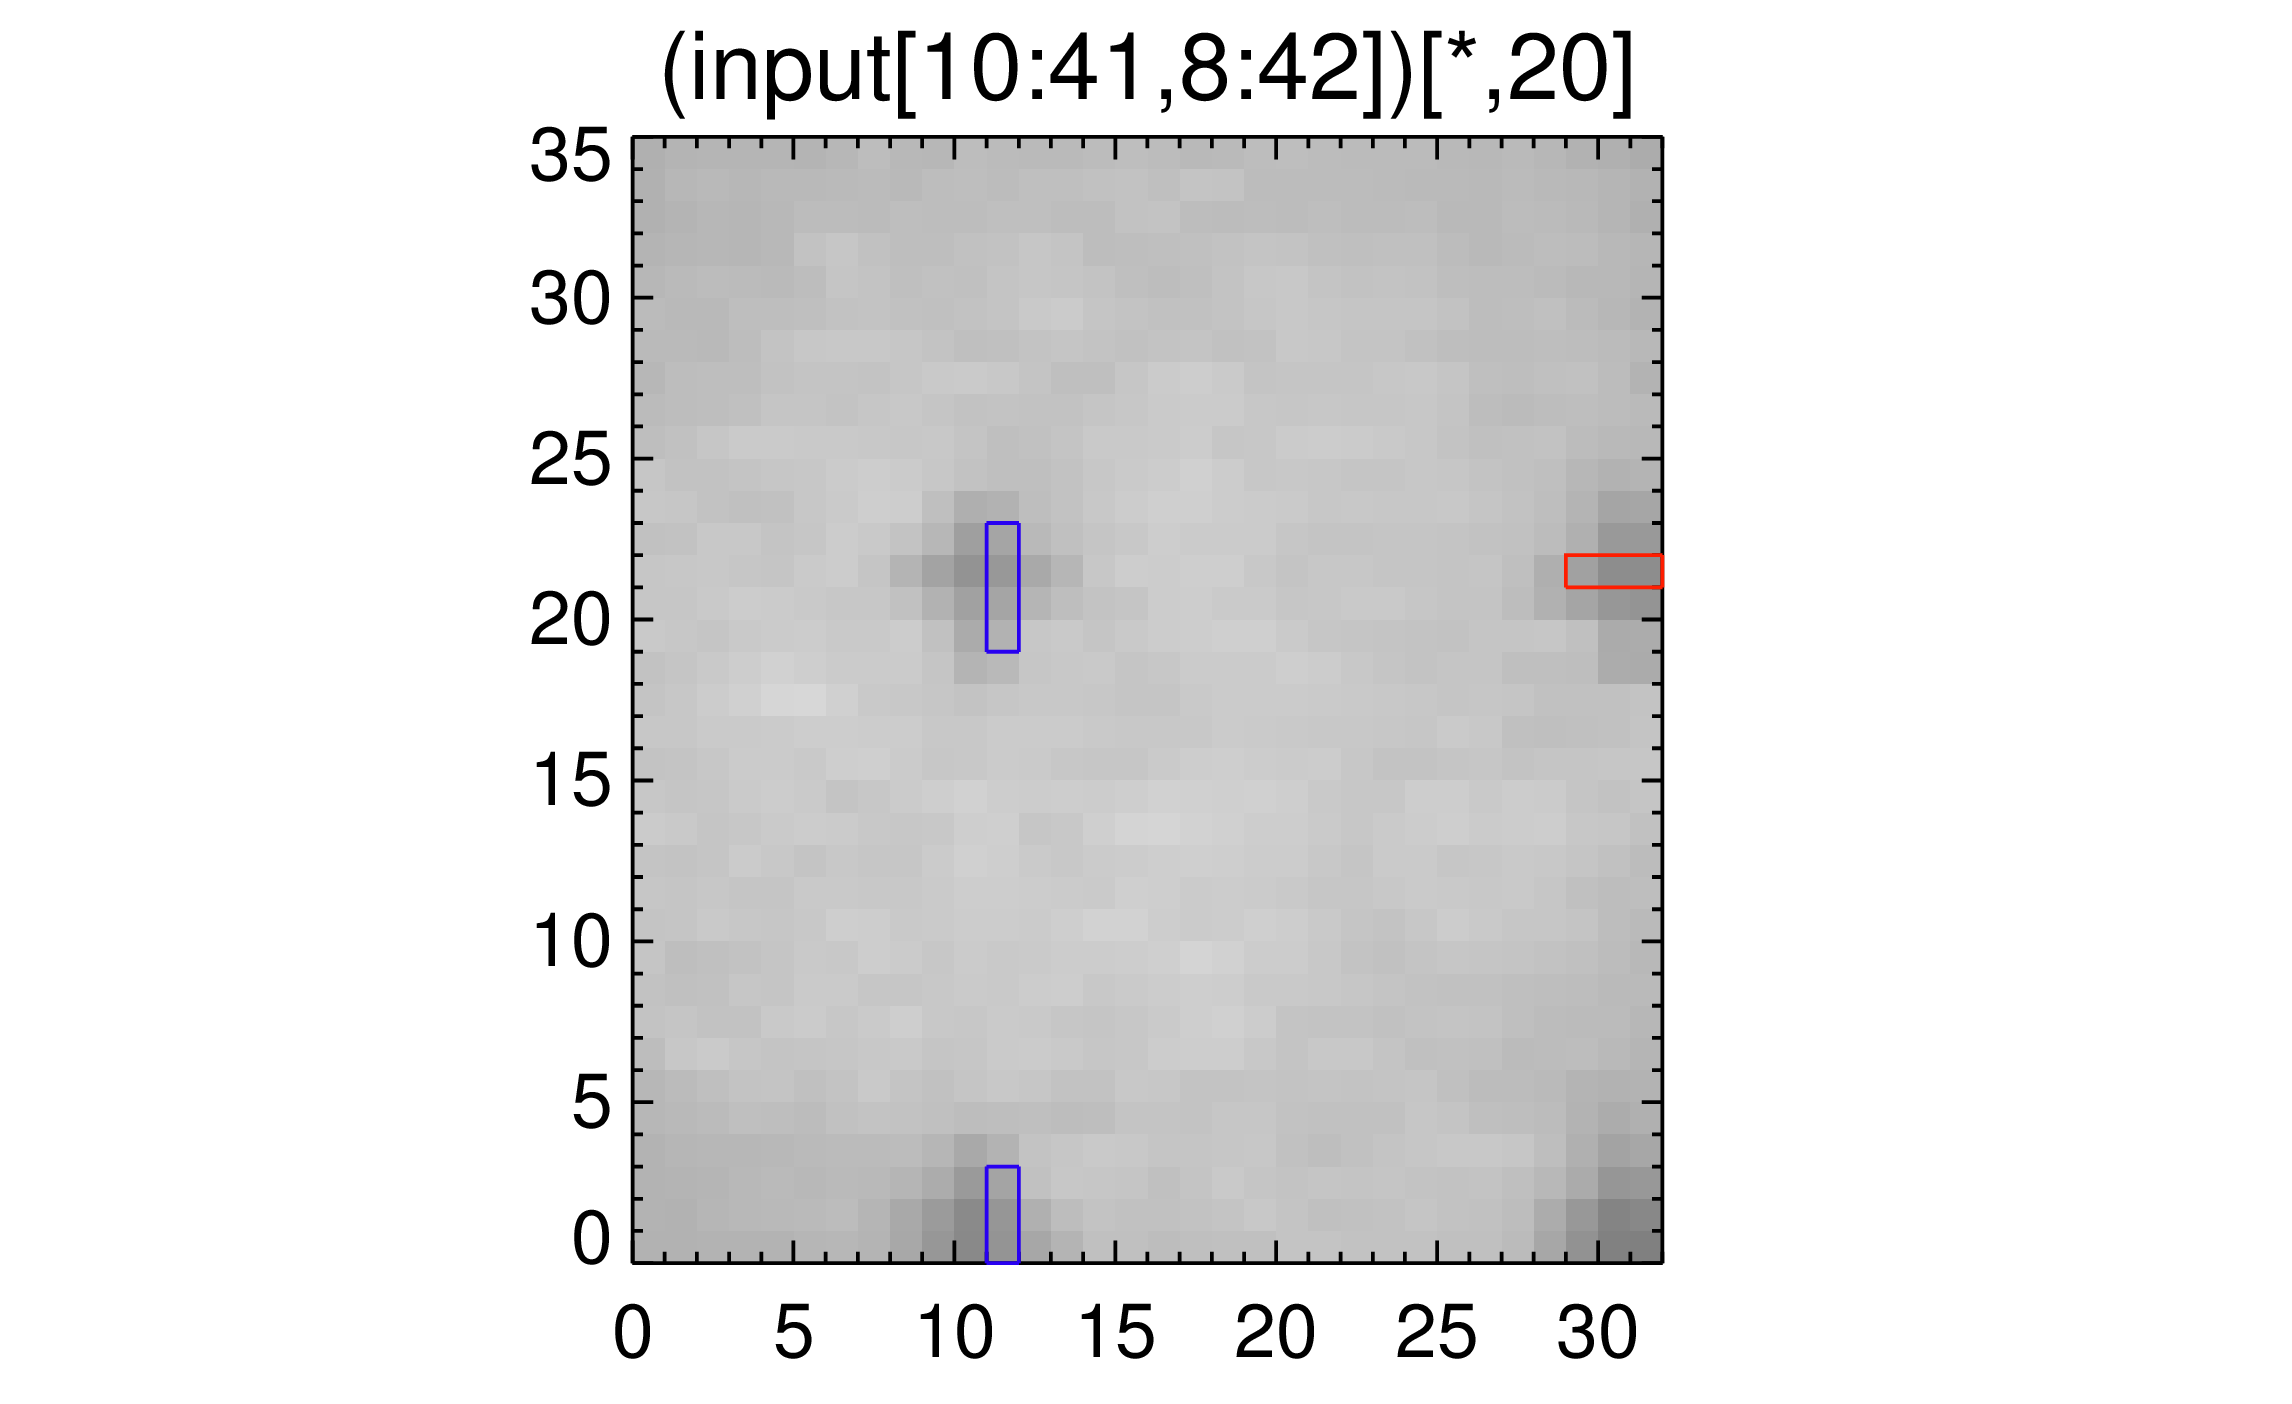
\includegraphics[width=1.3\textwidth]{../plots_tables_images/fidcheck_withbothtruncate3.png}
%         \caption{4 pixels}
%     \end{subfigure}

%     \begin{subfigure}[b]{.45\linewidth}
%         \centering
%         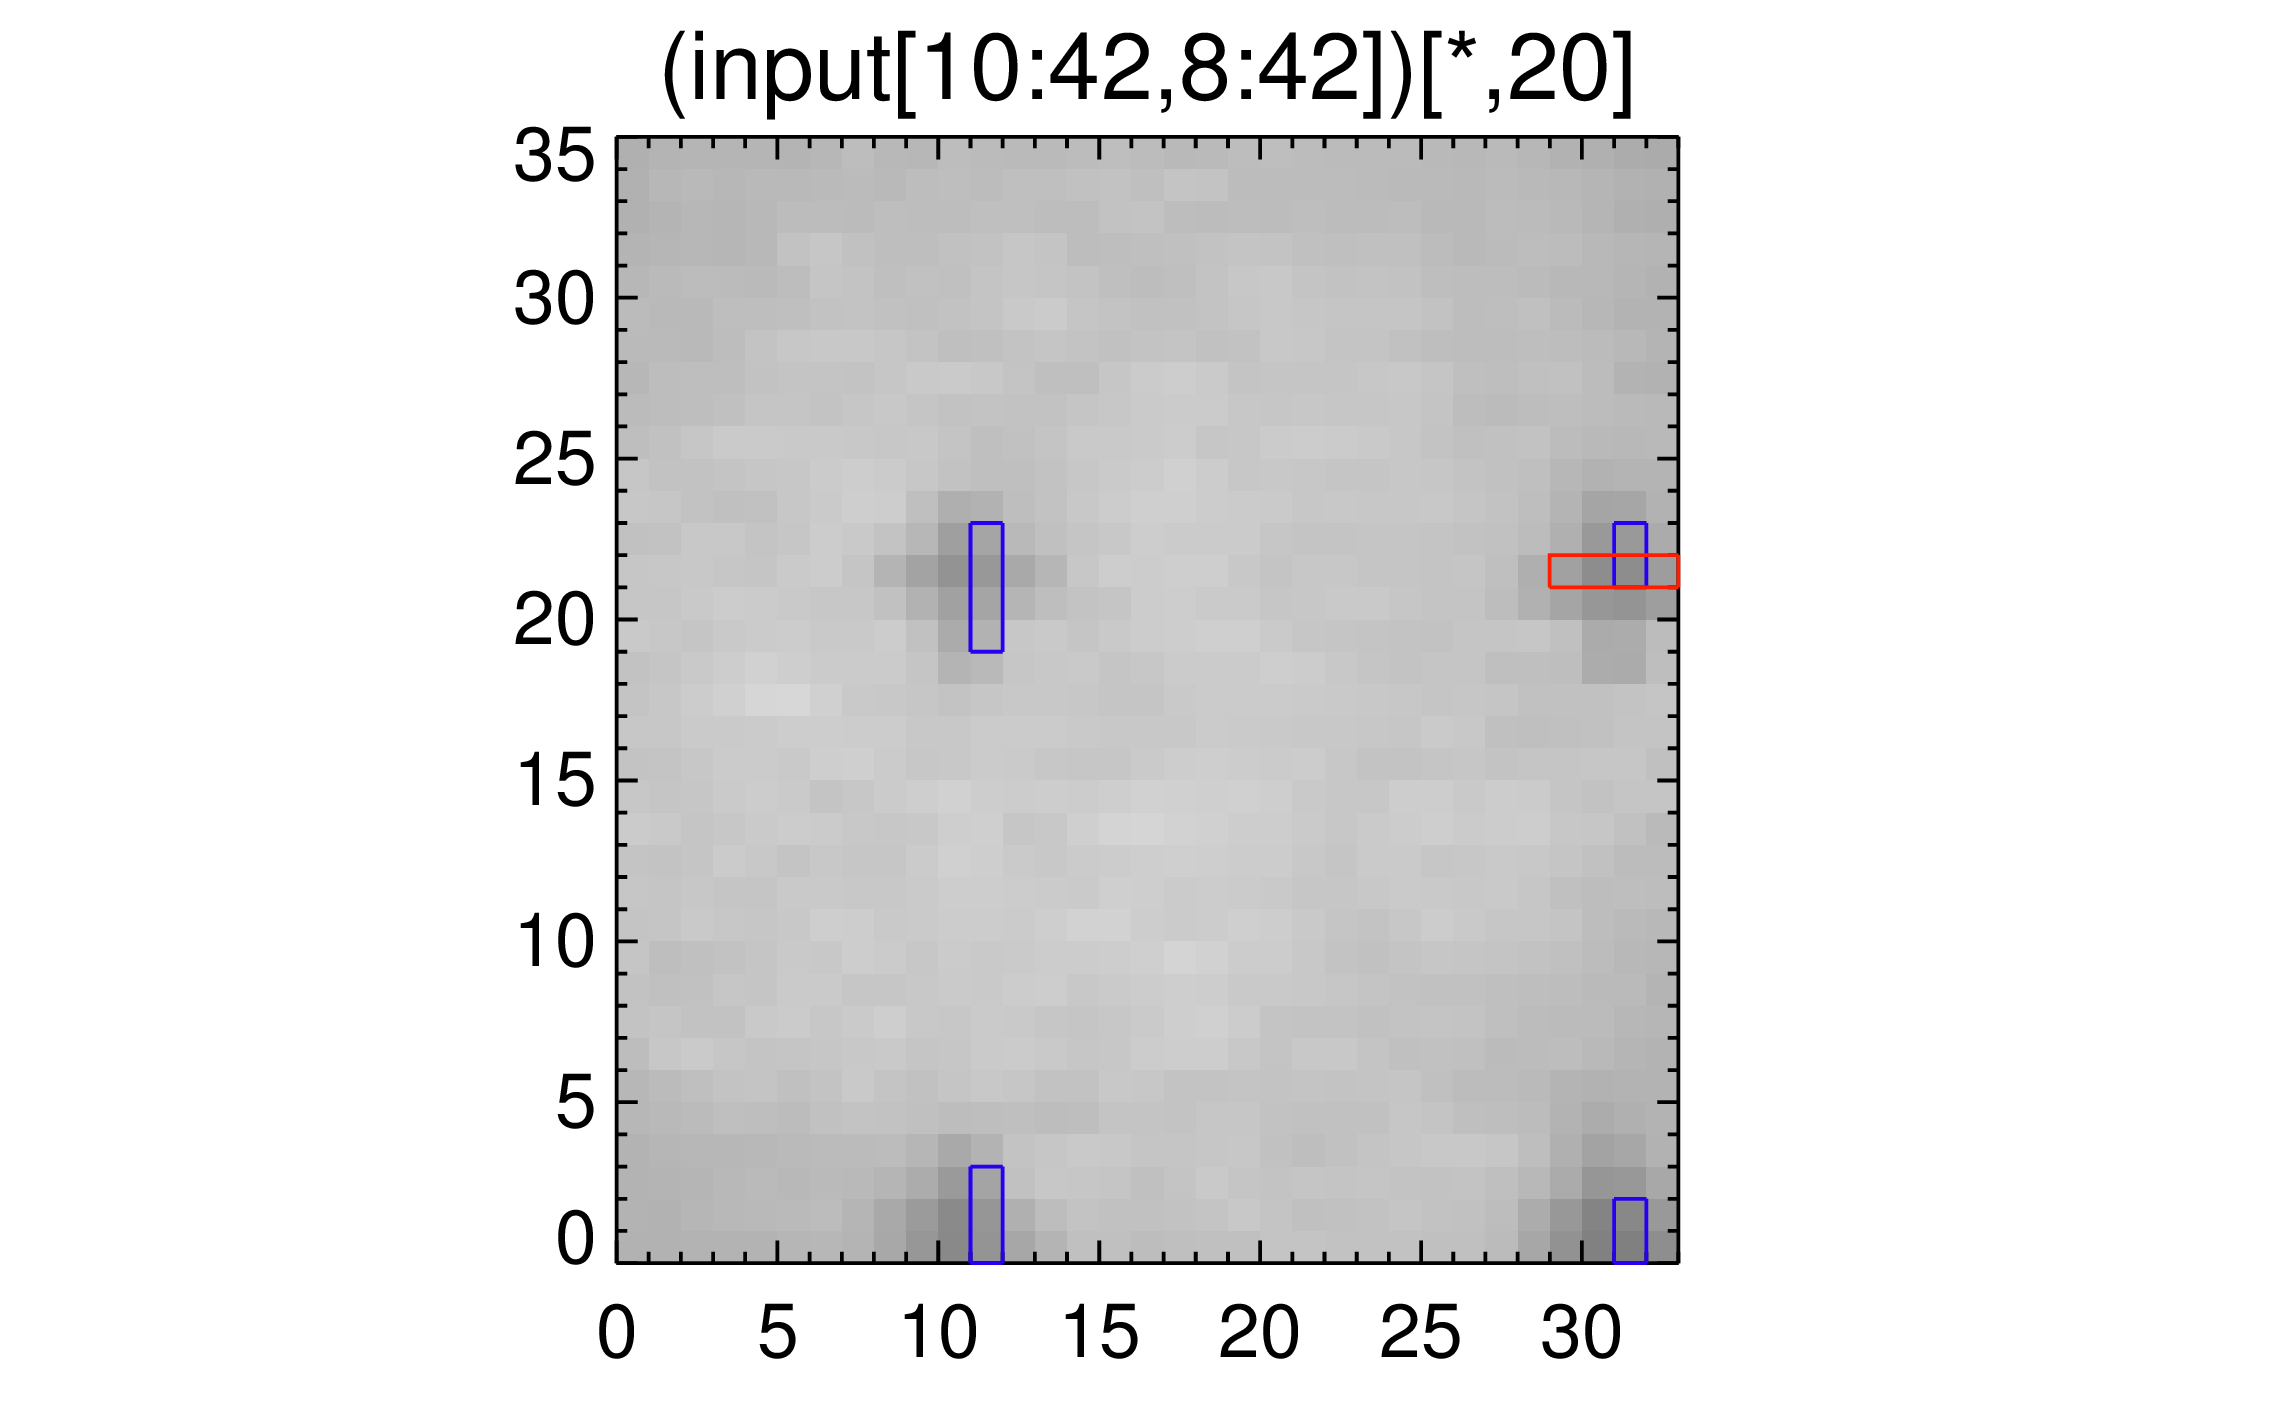
\includegraphics[width=1.3\textwidth]{../plots_tables_images/fidcheck_withbothtruncate4.png}
%         \caption{5 pixels}
%     \end{subfigure}
%     \begin{subfigure}[b]{.45\linewidth}
%         \centering
%         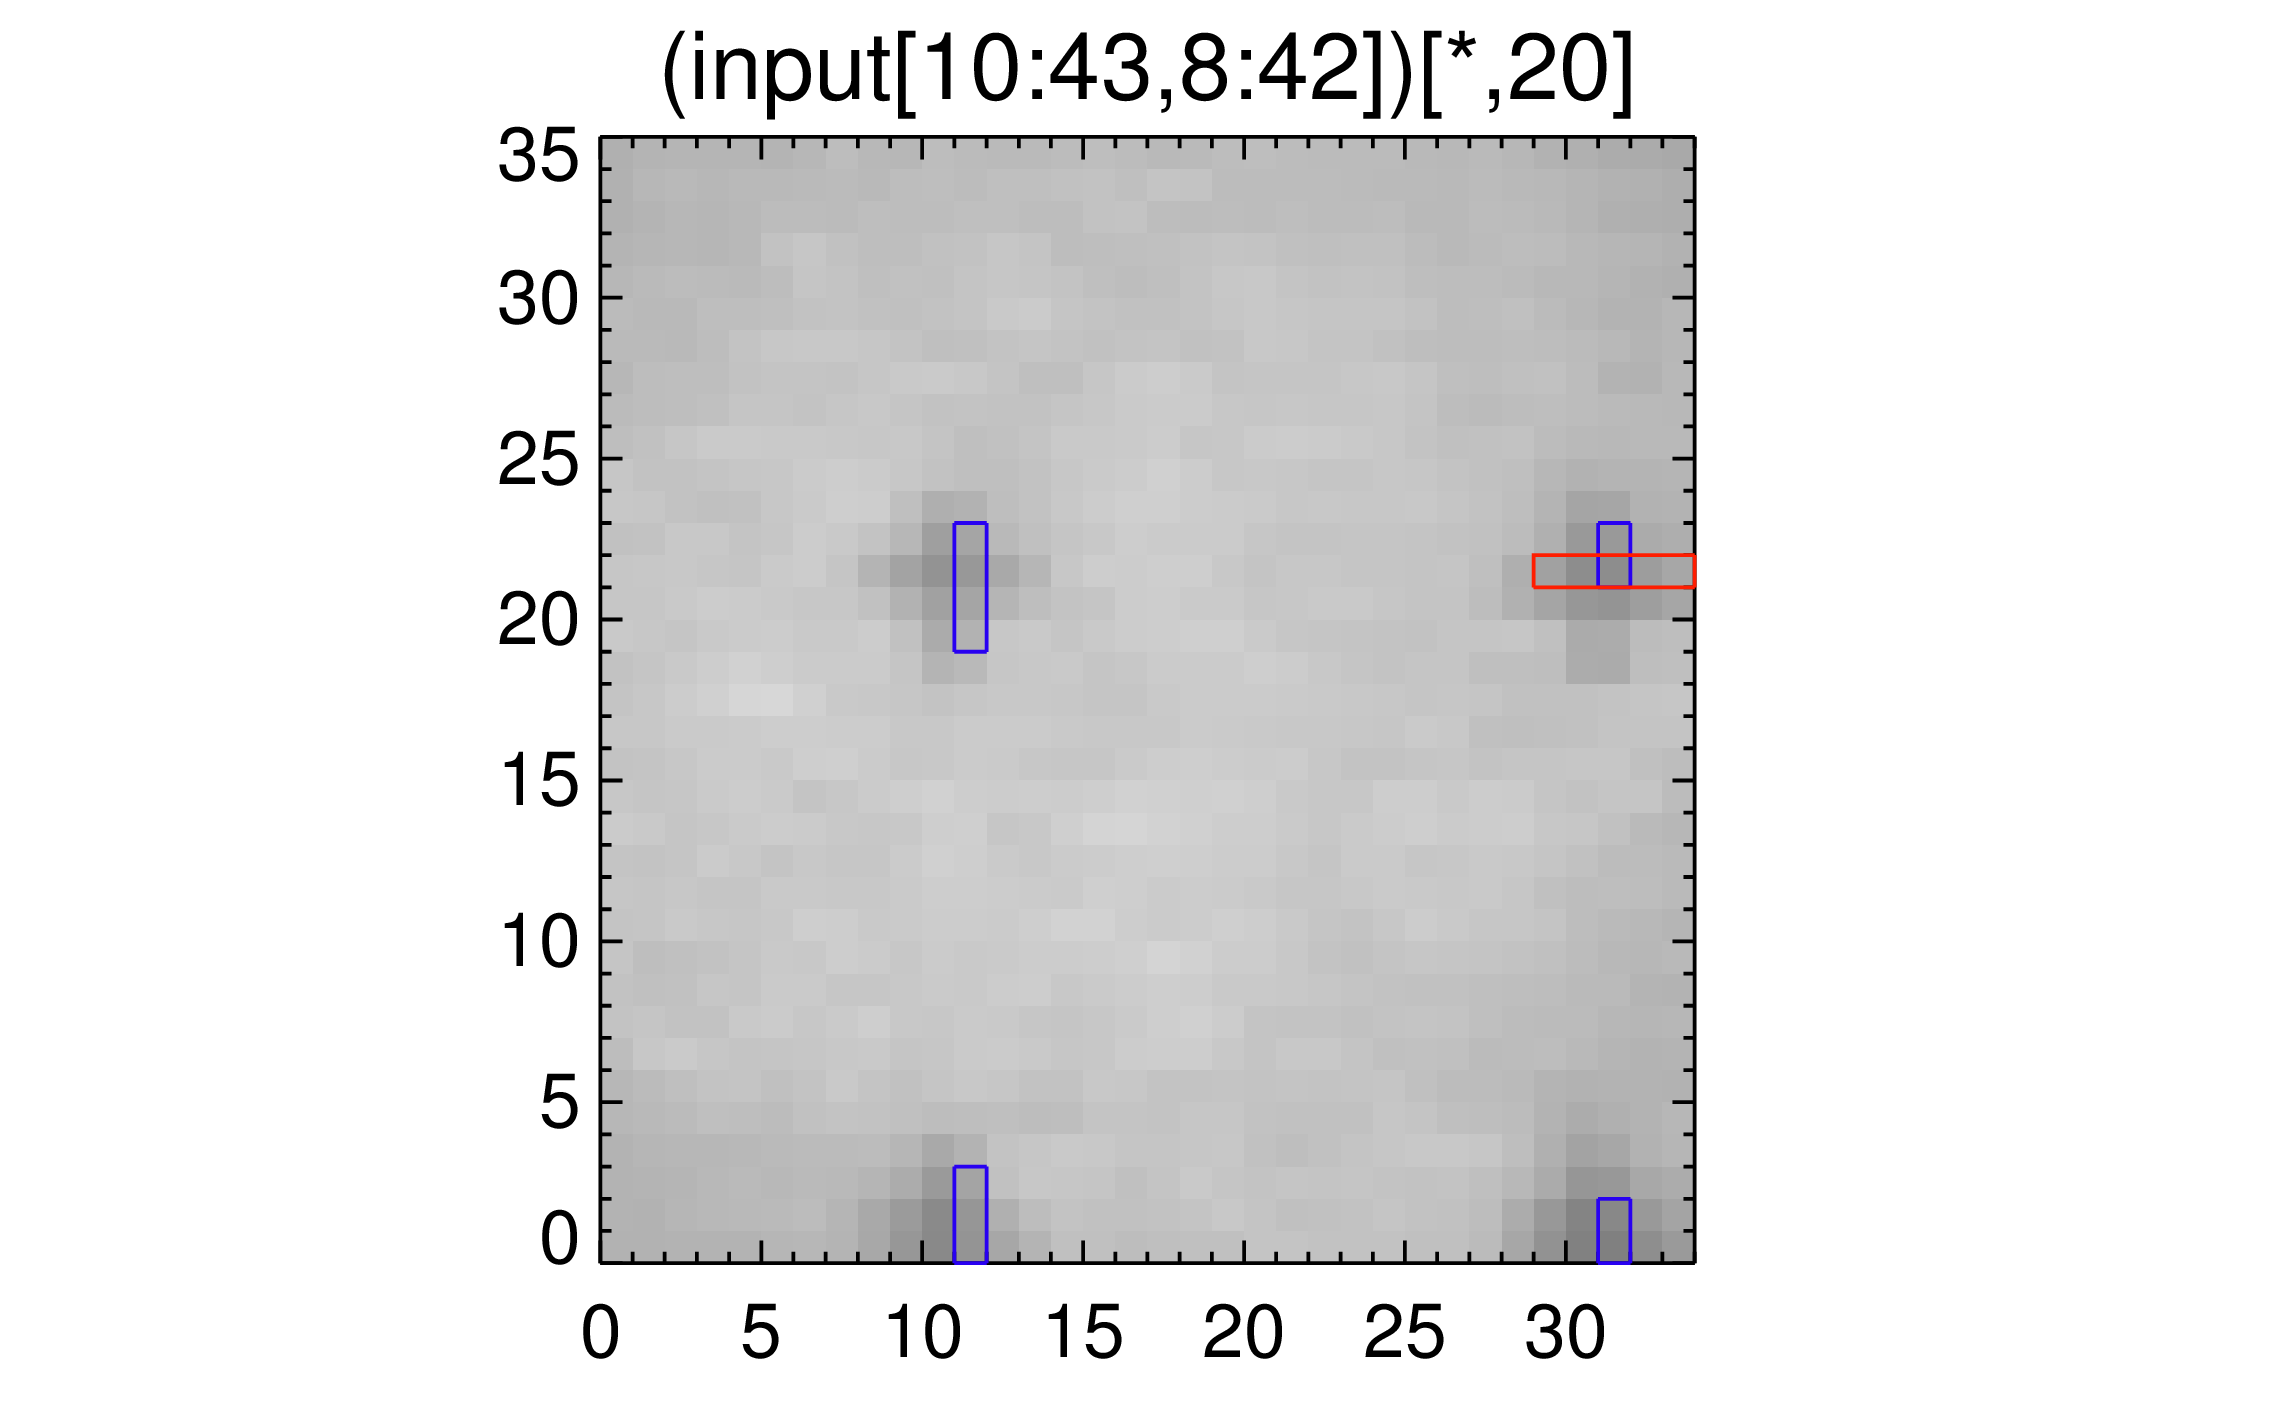
\includegraphics[width=1.3\textwidth]{../plots_tables_images/fidcheck_withbothtruncate5.png}
%         \caption{Completely in image}
%     \end{subfigure}
%     \caption{Result of \hl{\texttt{shift\_diff(emboss(image,/edge\_truncate),/edge\_truncate)}}. The top left is the most cropped image and the bottom right is the least cropped image.}
%     \label{firstplot}
% \end{figure}

Figure \ref{firstplot} reveals a basic check to see at what crop size do the convolution filters fail to return a fiducial position. 

\subsection{edge\_truncate} % (fold)
\label{sub:edge_truncate}
I will point out here that it is important to have the \hl{\texttt{edge\_truncate}} keyword set for the convolution filters. Here is an example in Figure \ref{whyedgetrunc}

\begin{figure}[!ht]
    \ffigbox[][\FBheight]{%
    \begin{subfloatrow}[2]%
        \ffigbox[\FBwidth]%
       {%
       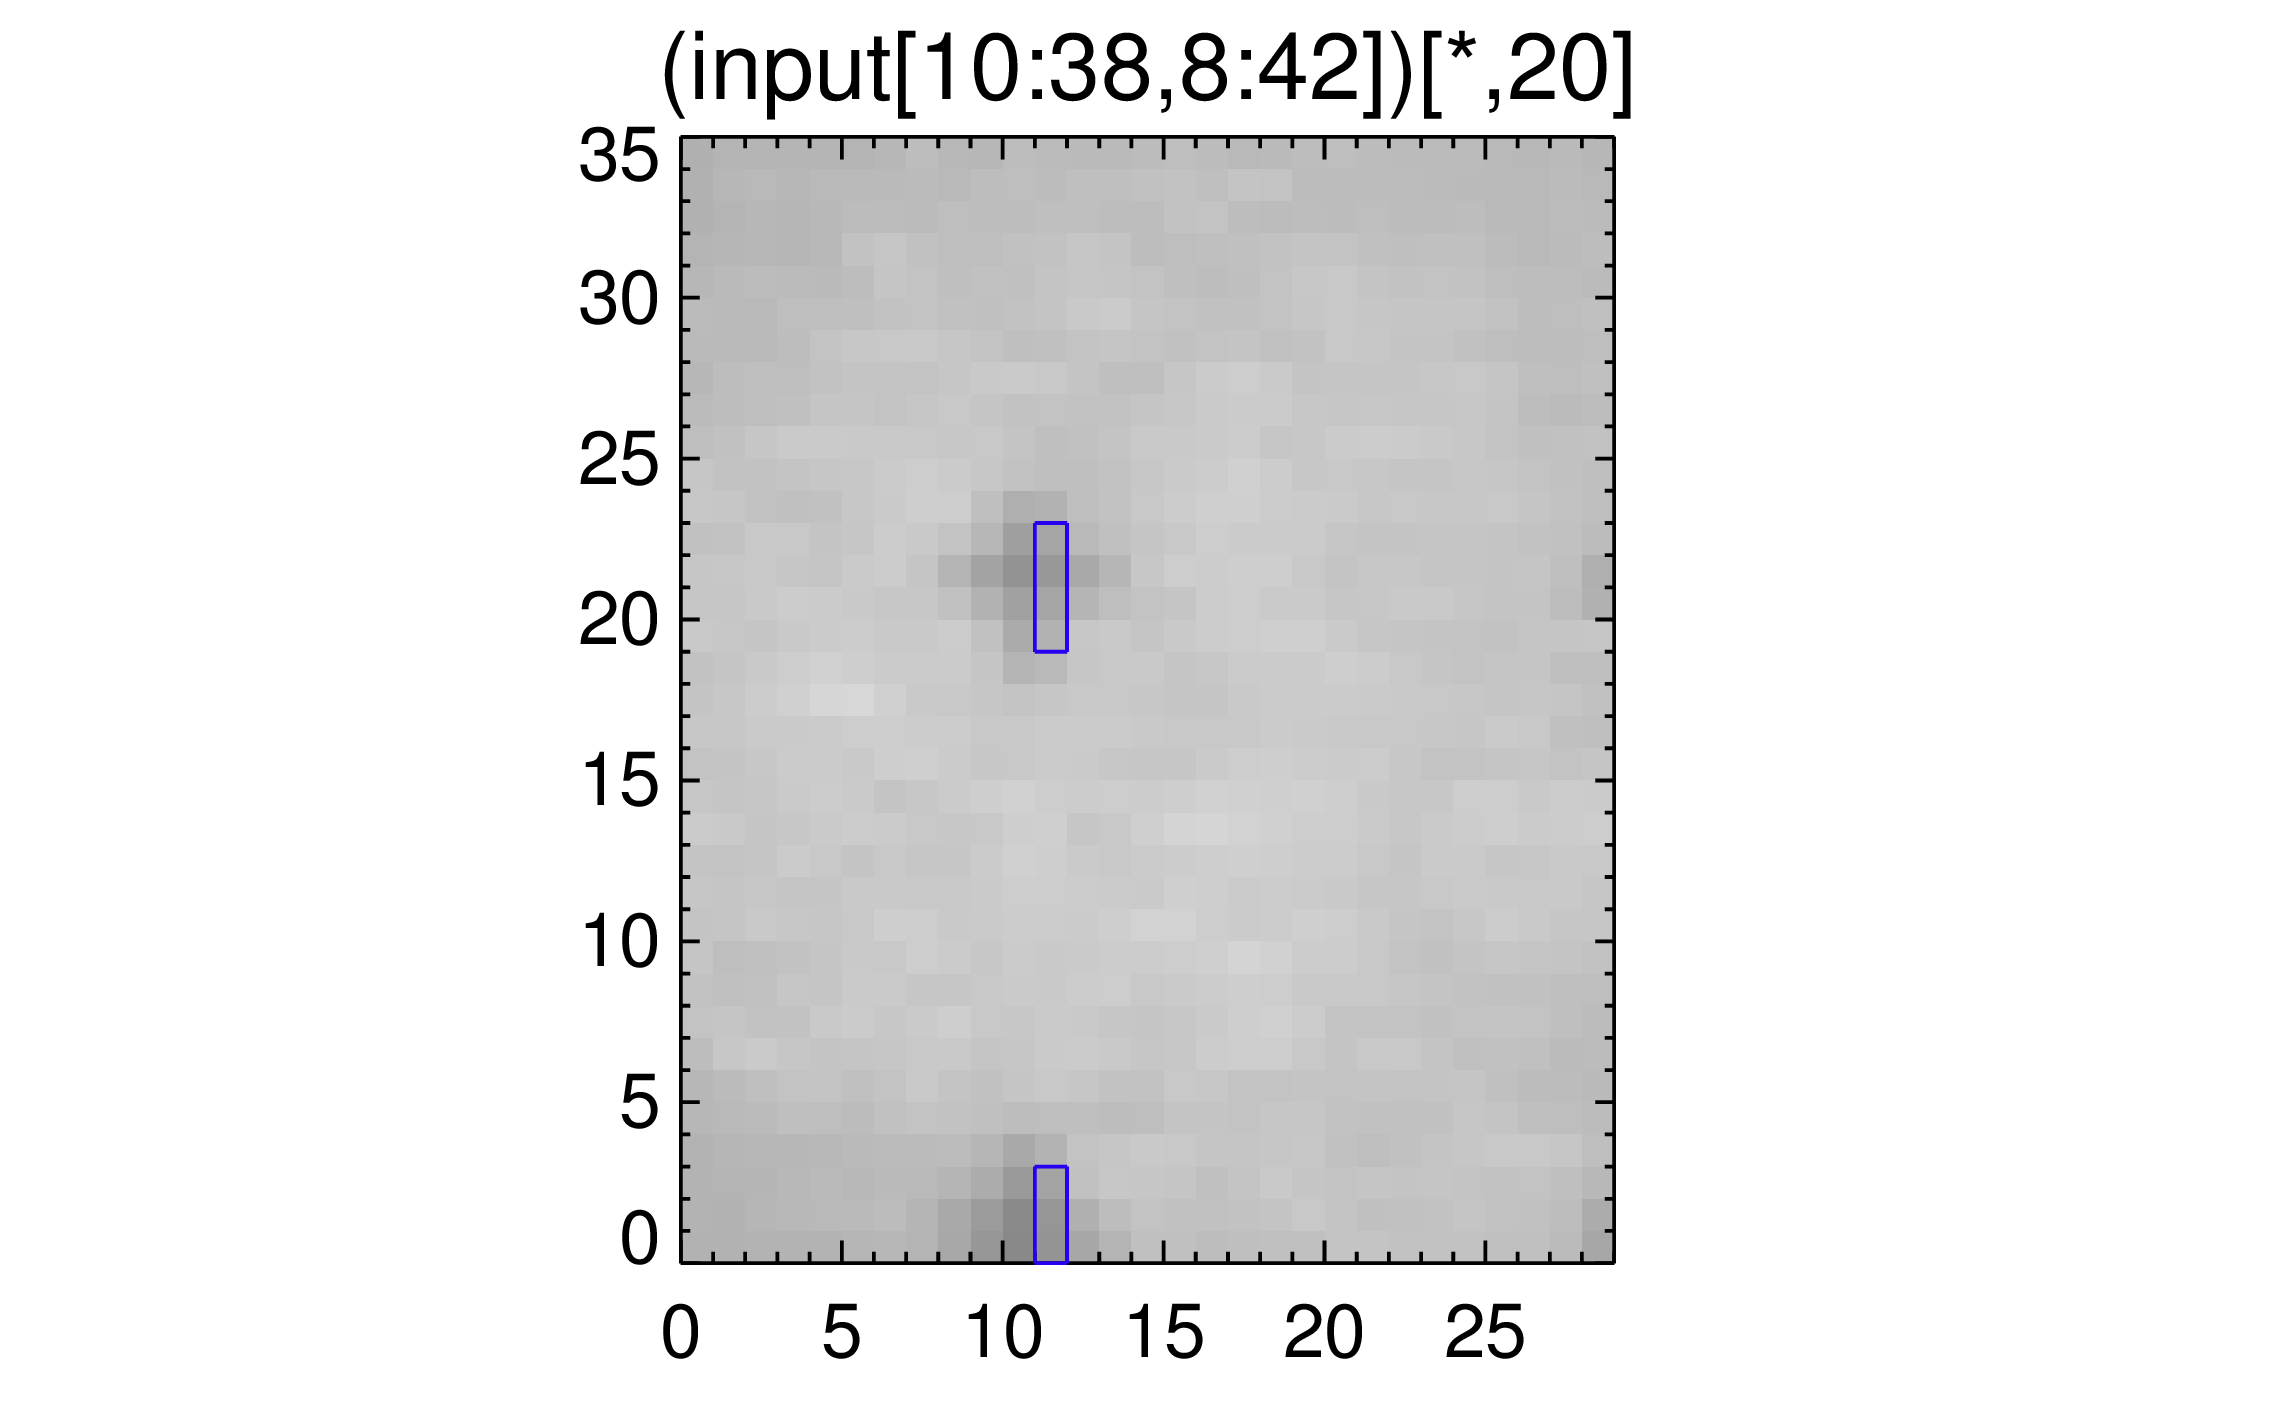
\includegraphics[width=.5\textwidth]{../plots_tables_images/fidcheck_withbothtruncate0.png}%
       }%
       {%
       \caption{Both filters have keyword}%
       }%
        \ffigbox[\Xhsize]%
       {%
       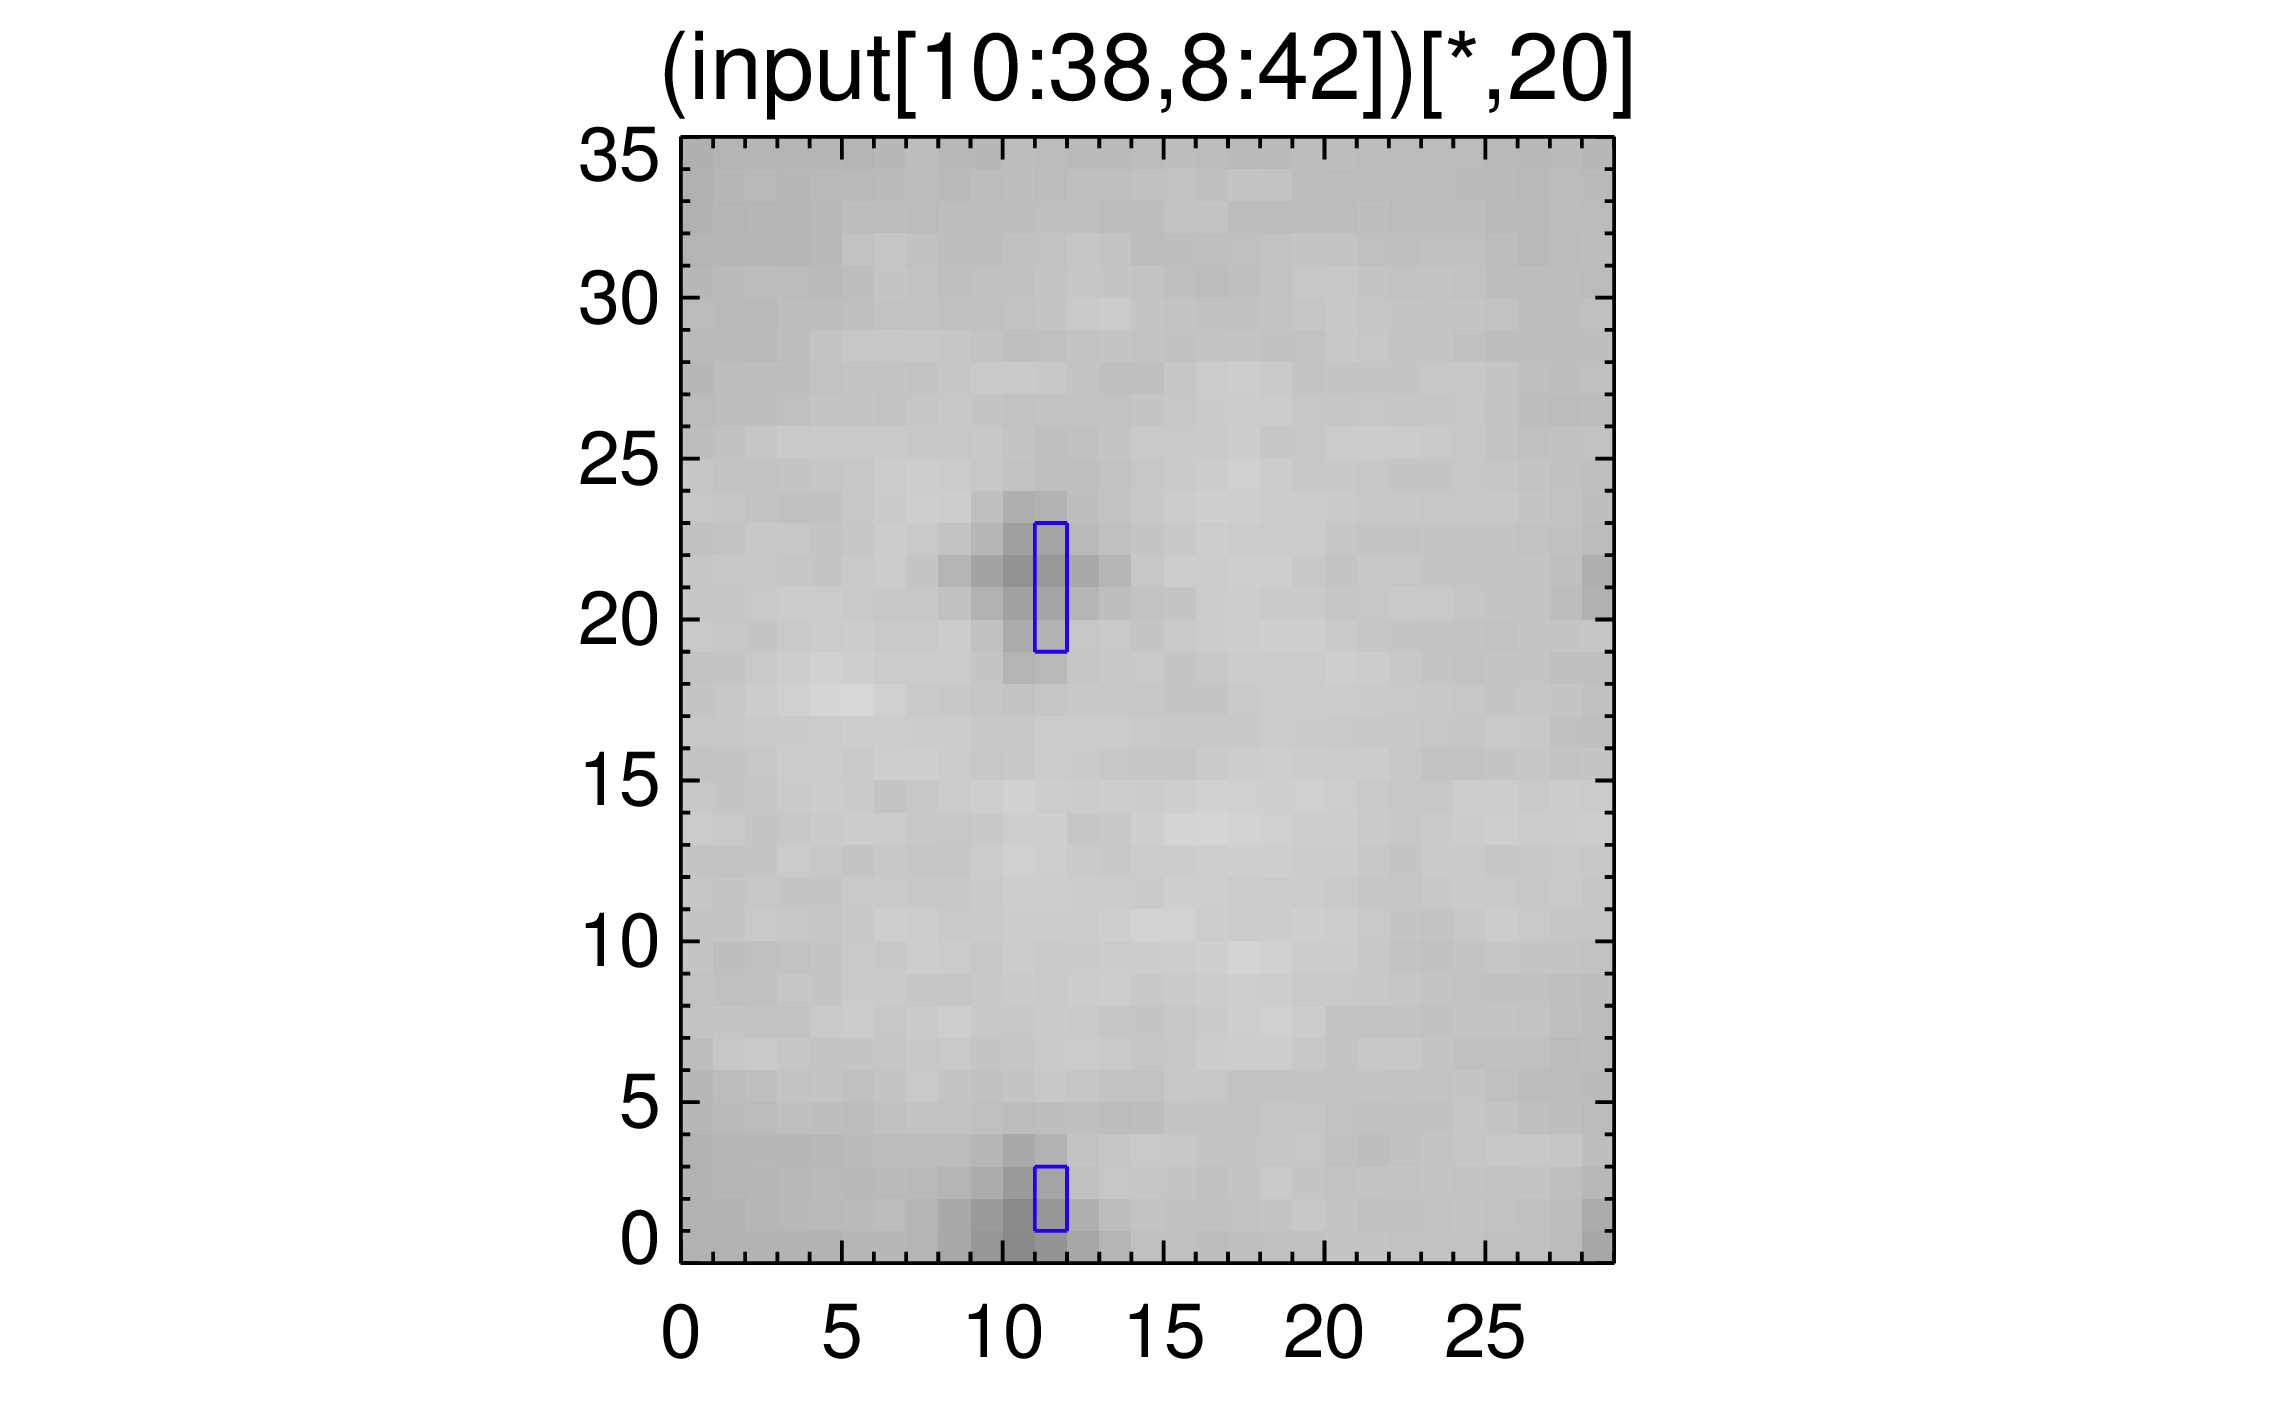
\includegraphics[width=.5\textwidth]{../plots_tables_images/fidcheck_withembosstruncate0.png}%
       }%
       {%
       \caption{Just emboss}%
       }%
    \end{subfloatrow}}

    \ffigbox[][\FBheight]{%
    \begin{subfloatrow}[2]%
        \ffigbox[\FBwidth]%
       {%
       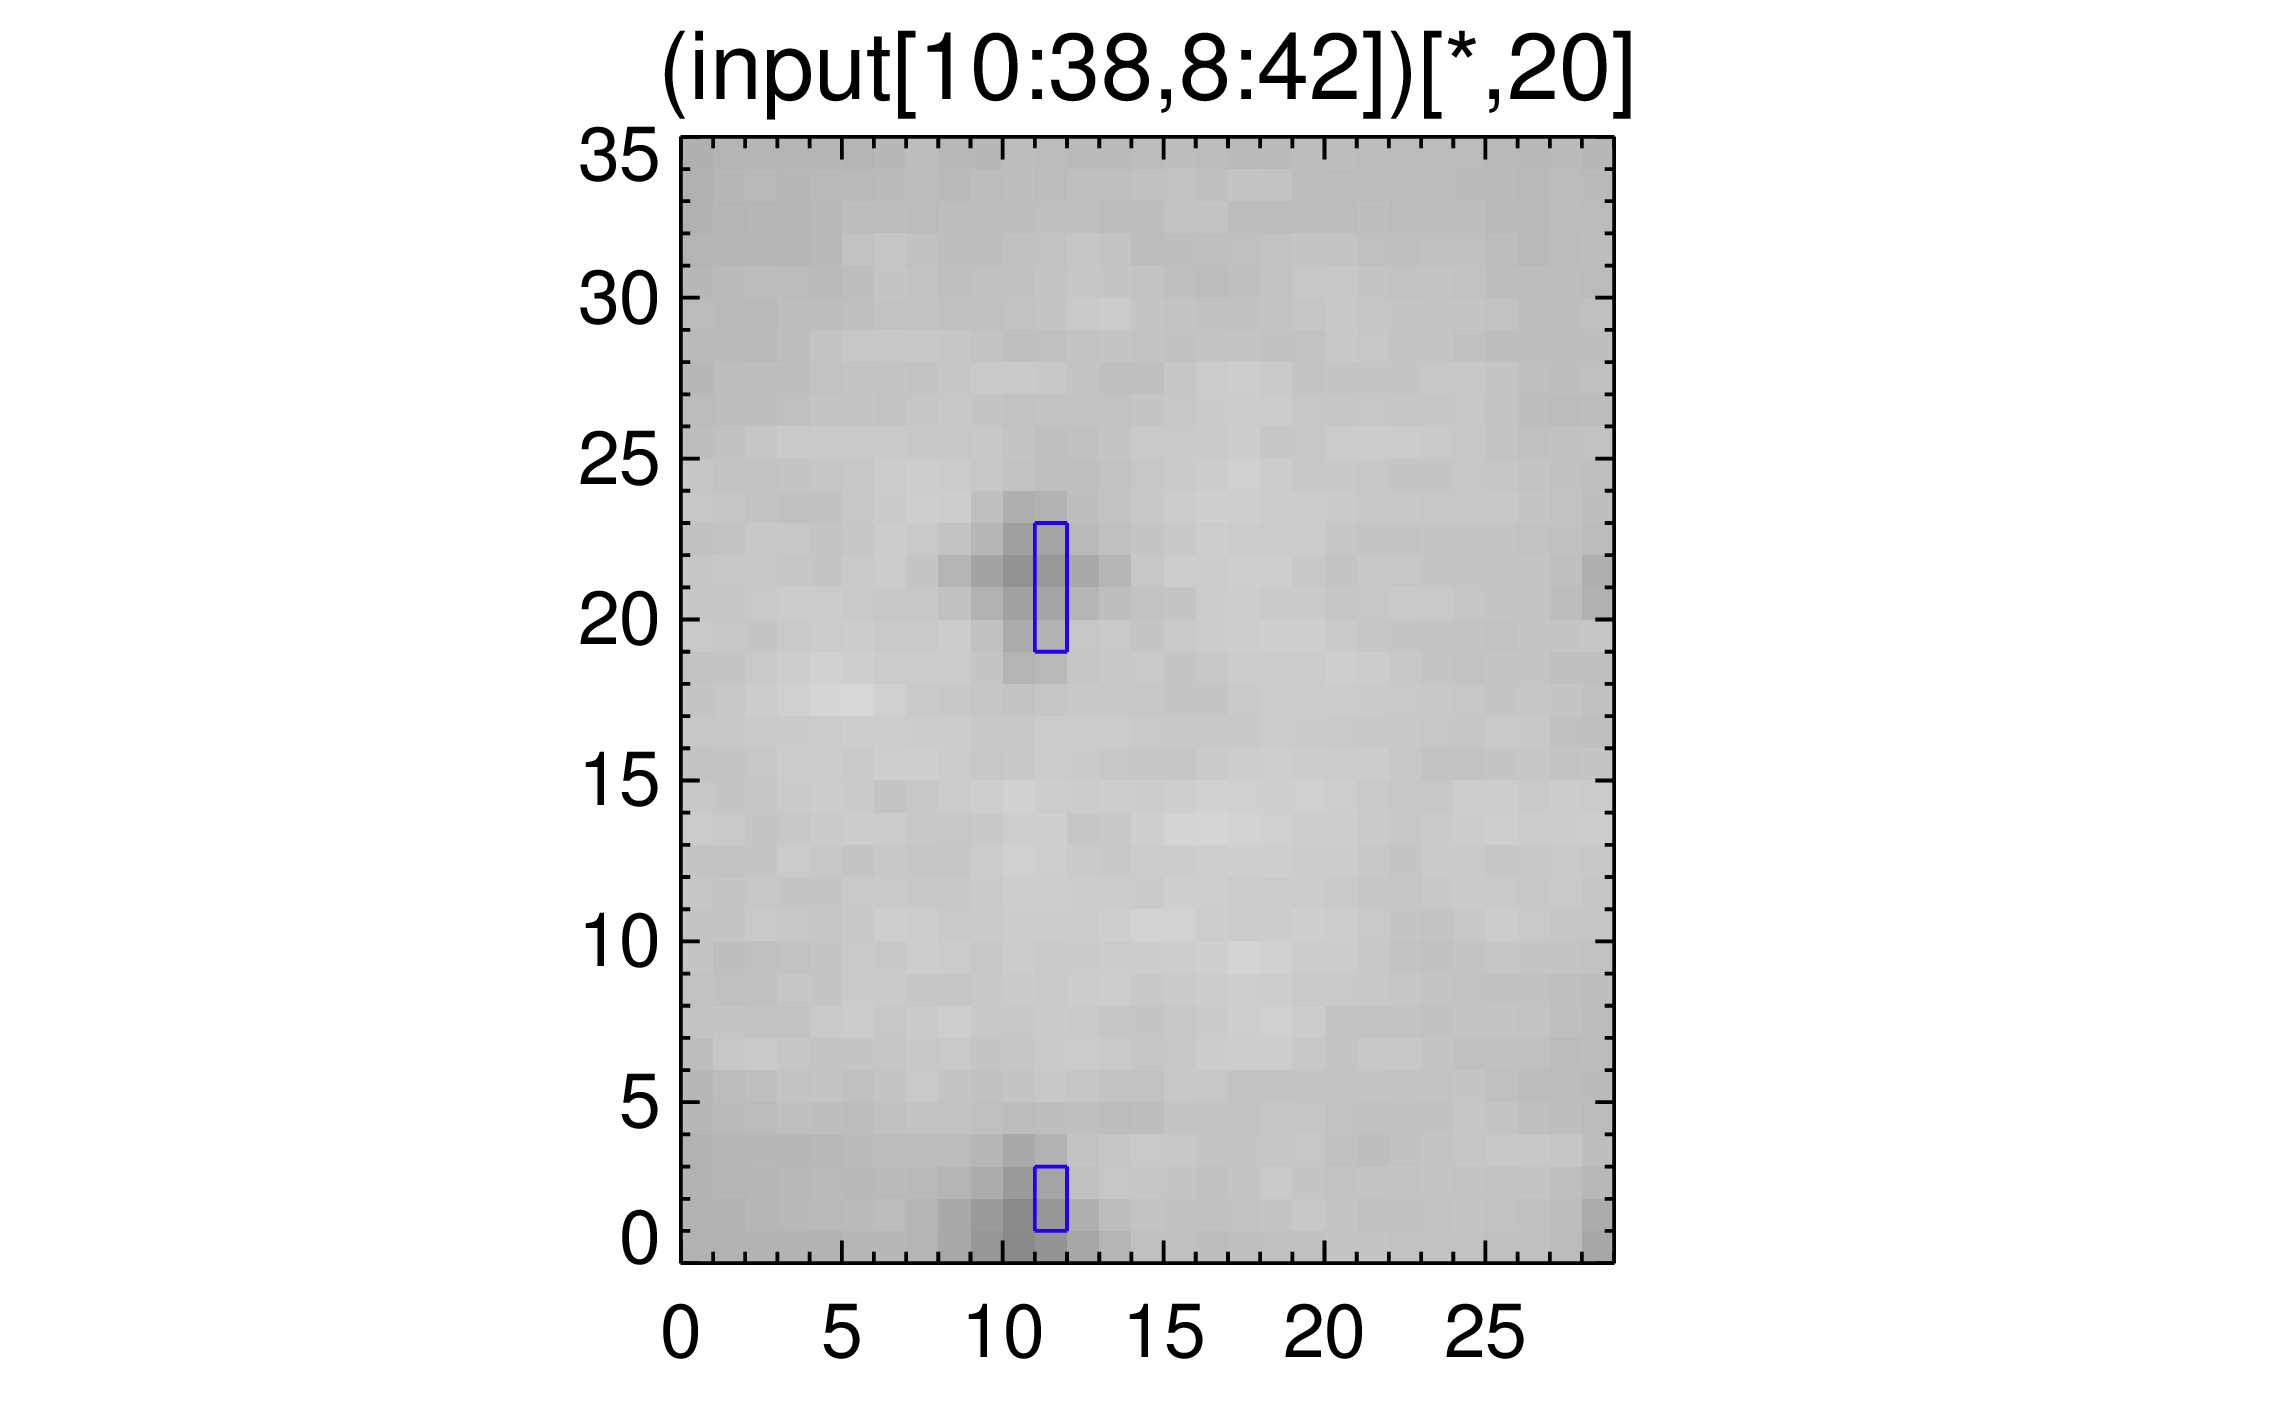
\includegraphics[width=.5\textwidth]{../plots_tables_images/fidcheck_withshiftdifftruncate0.png}%
       }%
       {%
       \caption{Just shift\_diff}%
       }%
        \ffigbox[\Xhsize]%
       {%
       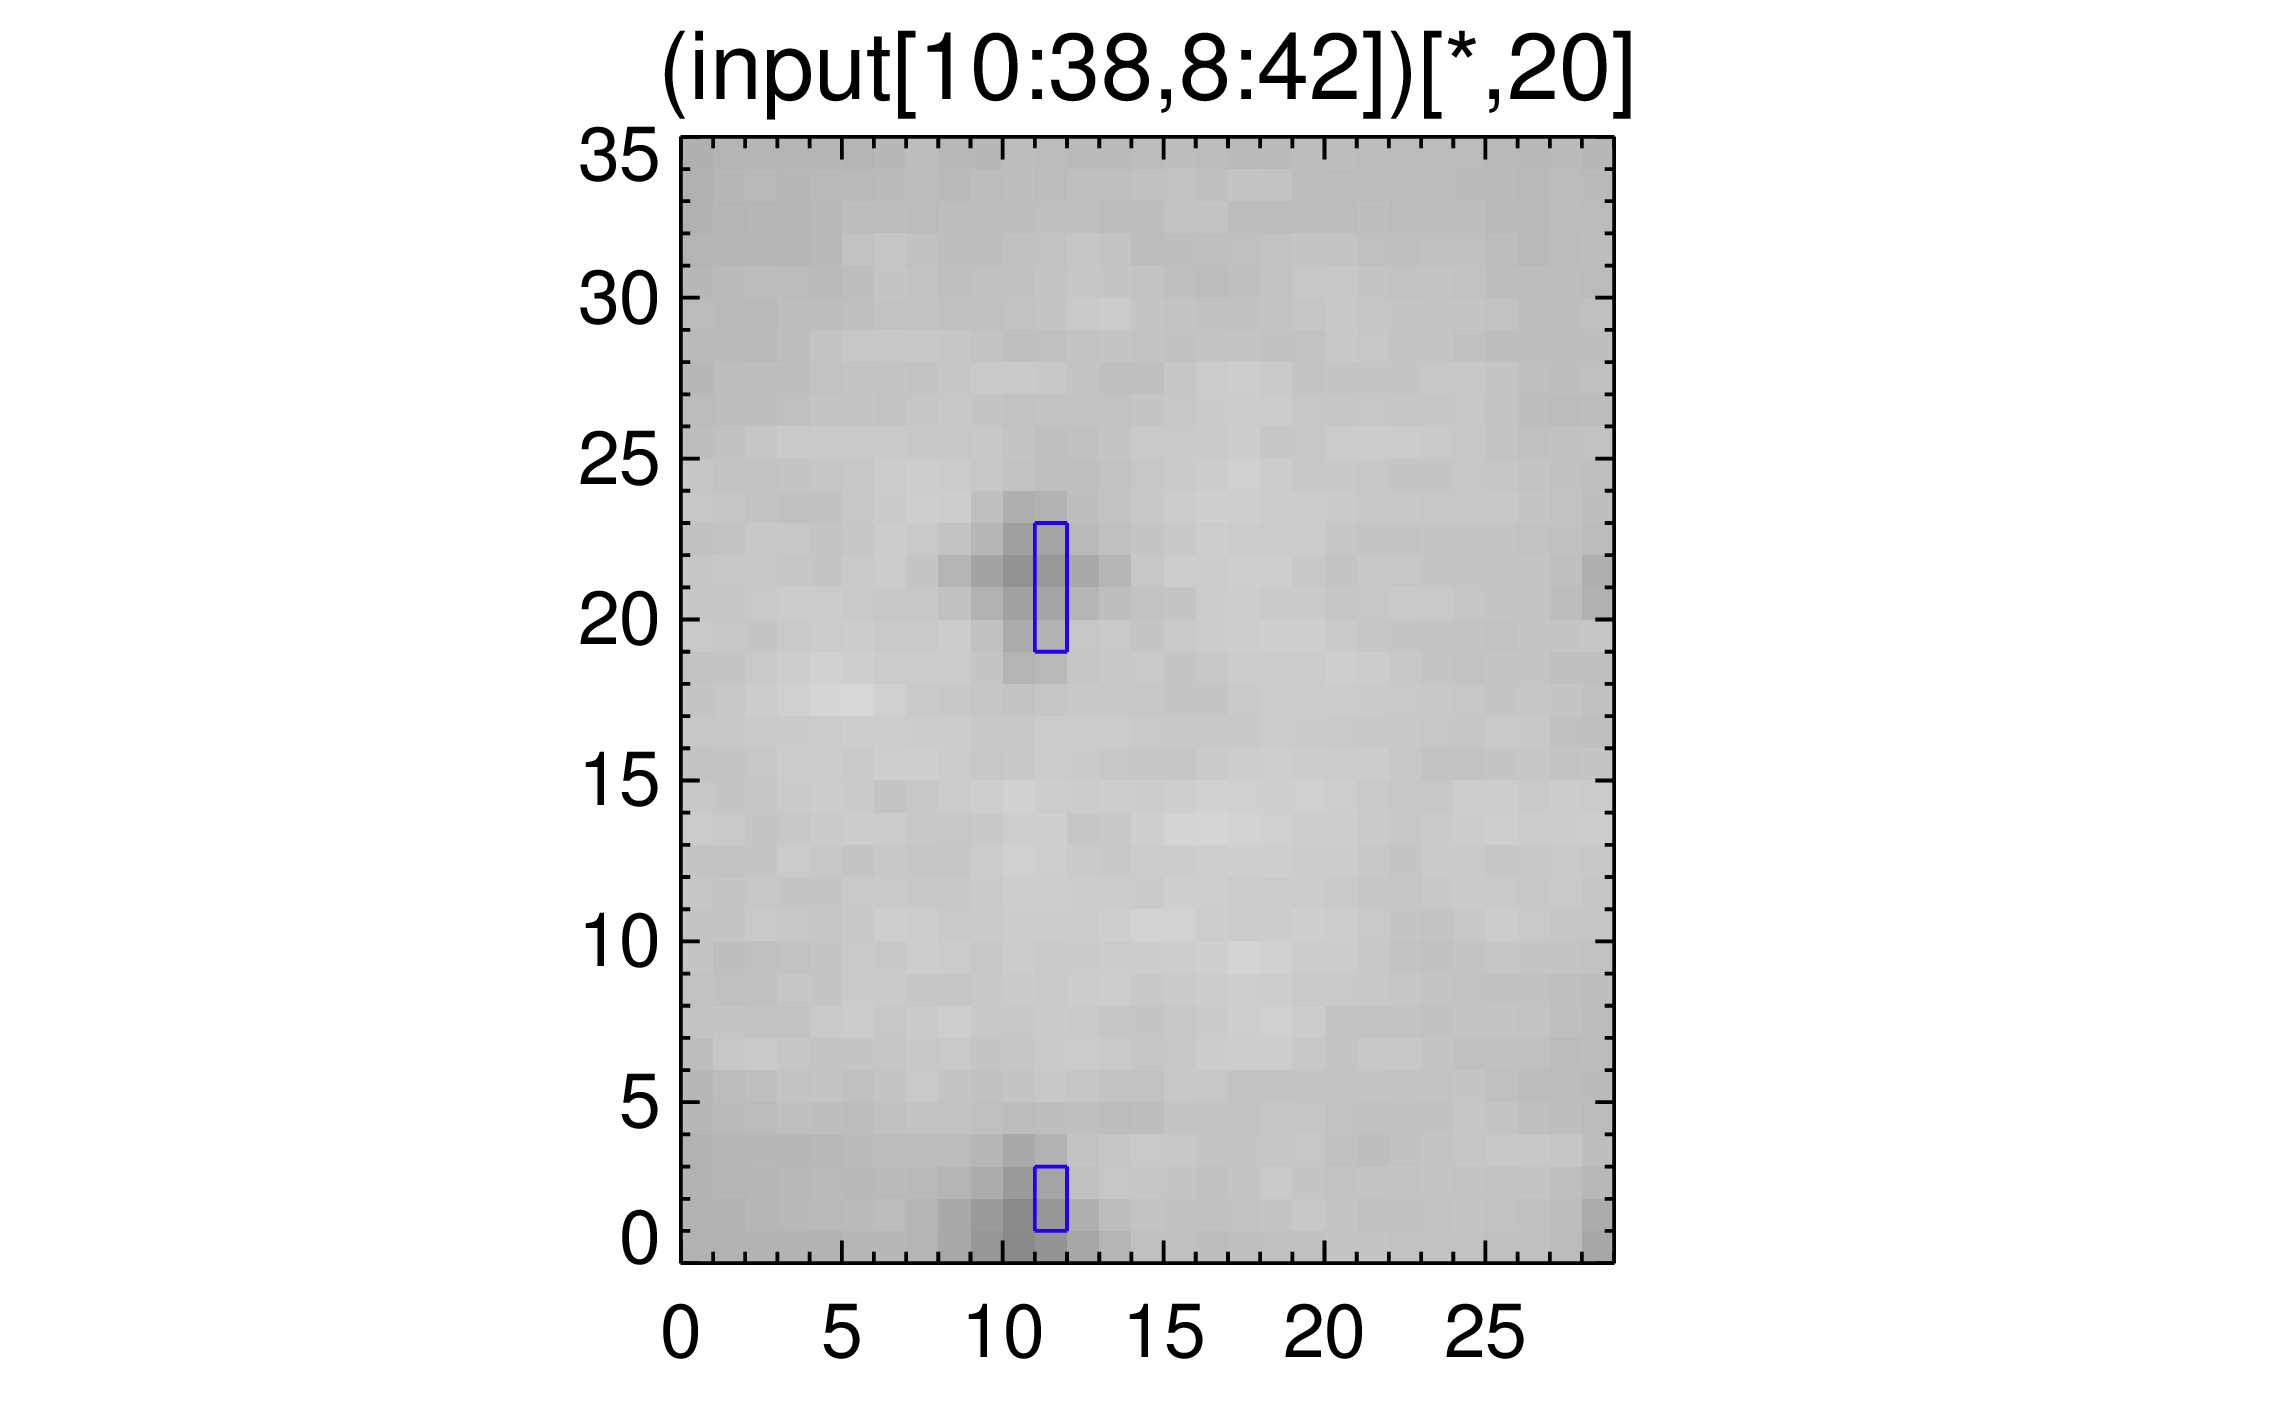
\includegraphics[width=.5\textwidth]{../plots_tables_images/fidcheck_withnotruncate0.png}%
       }%
       {%
       \caption{No keywords}%
       }%
    \end{subfloatrow}}{\caption{Only one of the images is different from the other. Can you guess which of the WHO THE WHAT NOW}\label{whyedgetrunc}}
\end{figure}

% \begin{figure}[!h]
%     \centering 
%     \begin{subfigure}[b]{.45\linewidth}
%         \centering
%         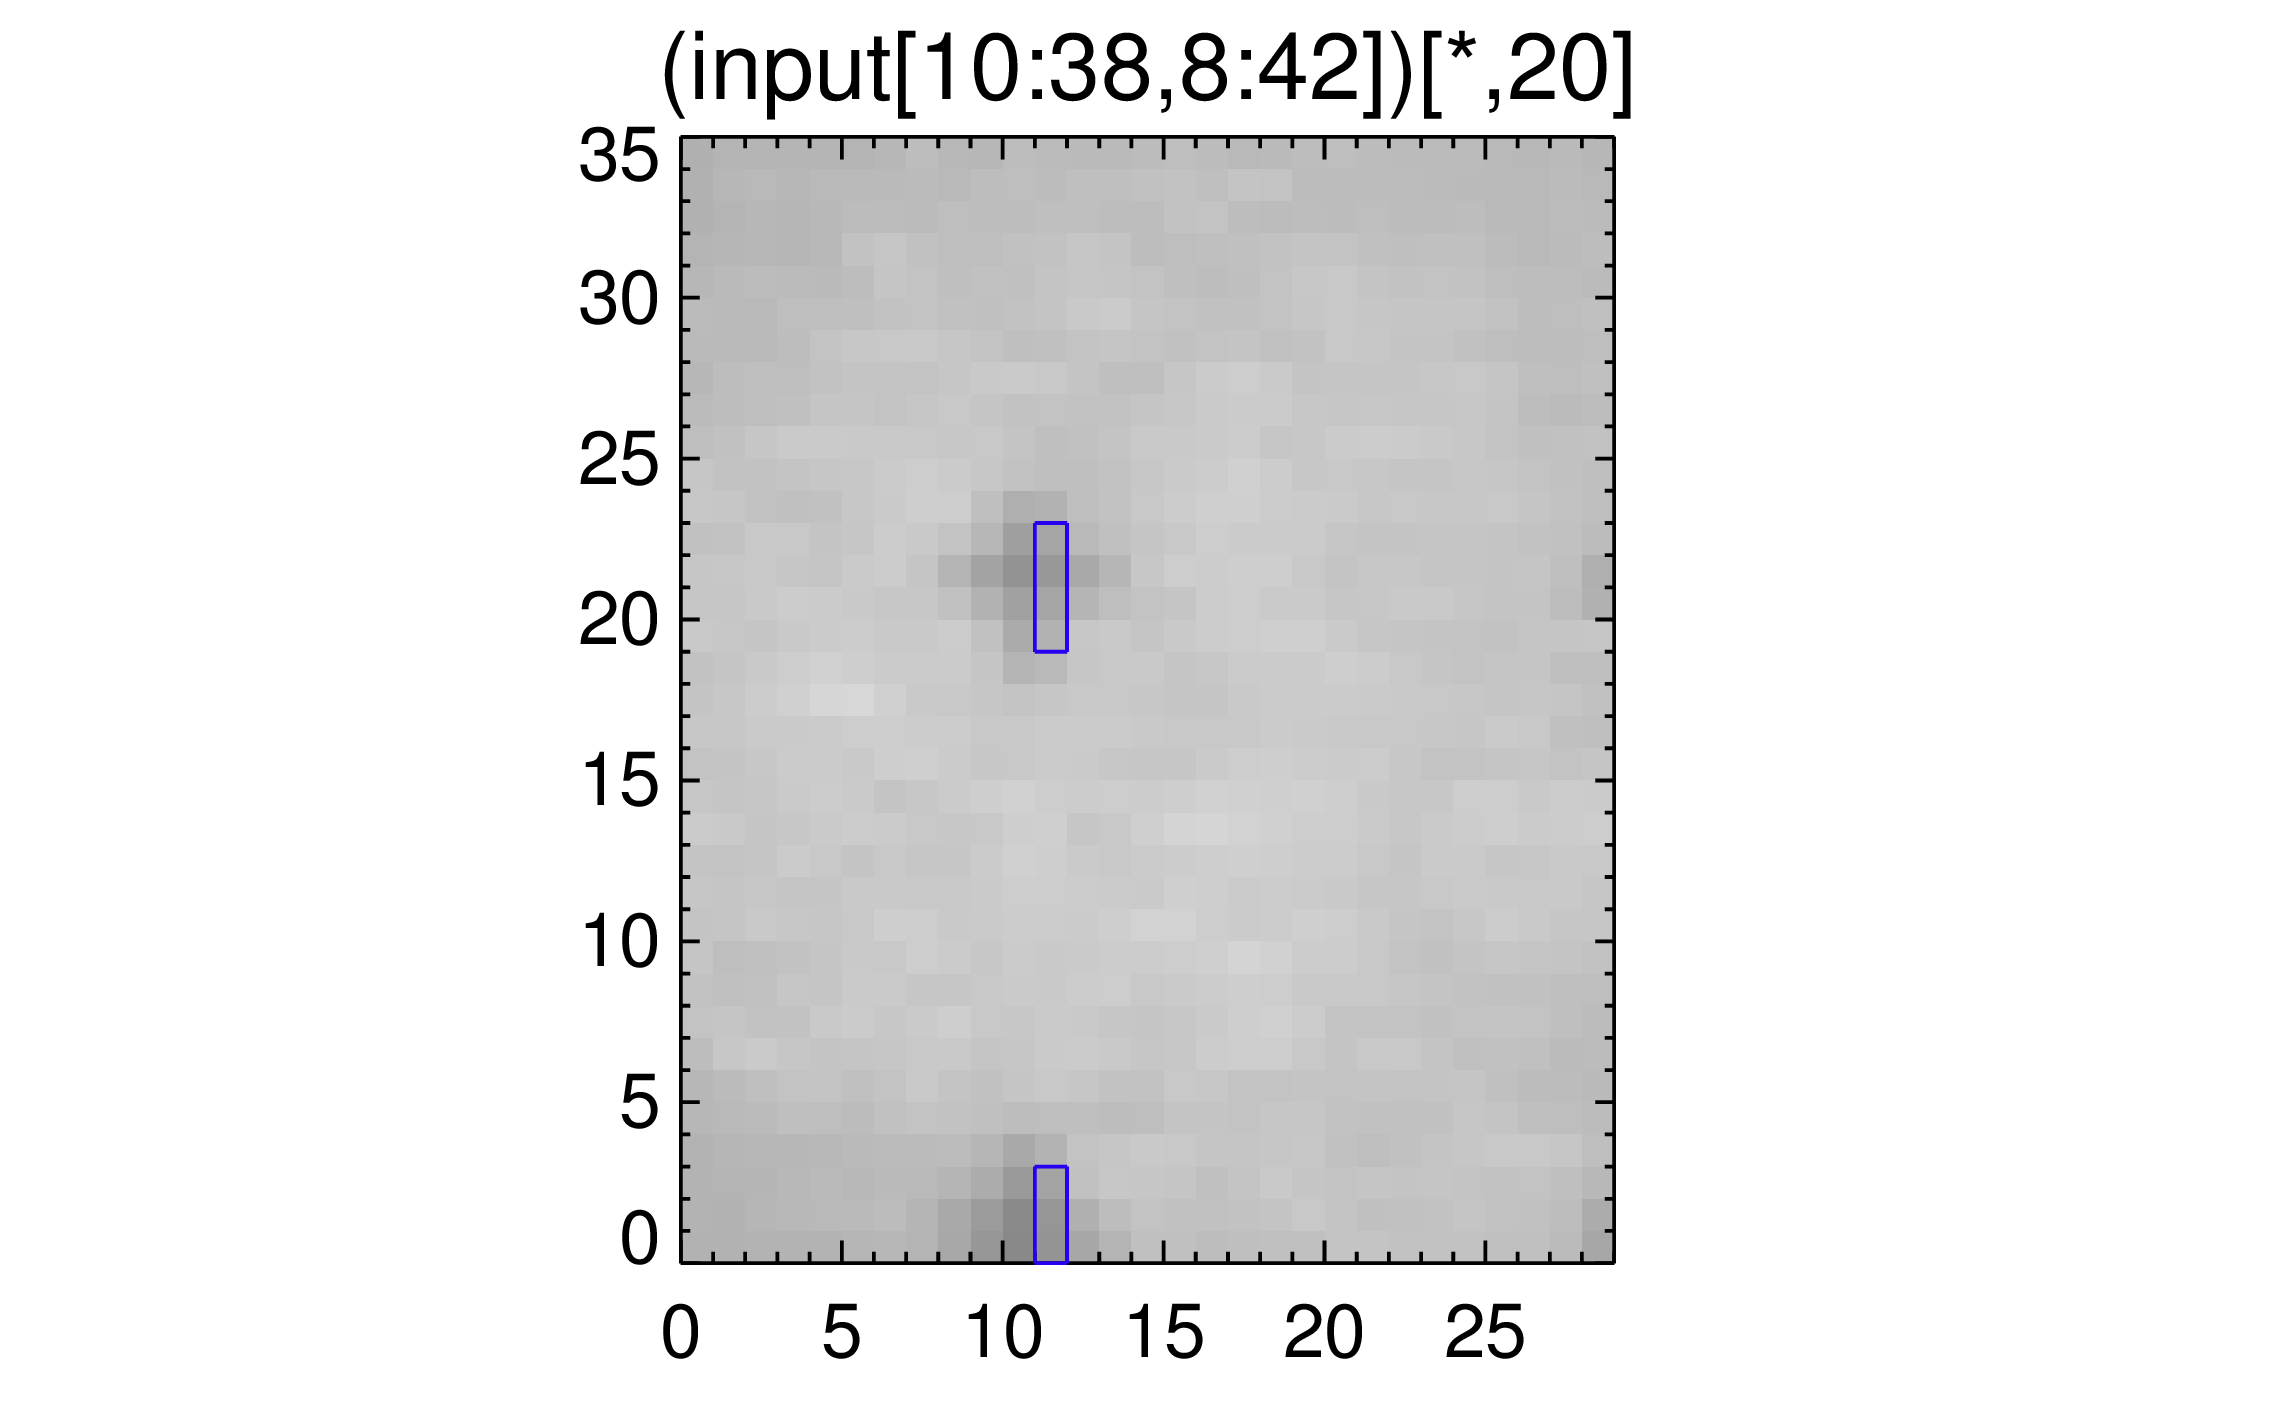
\includegraphics[width=1.3\textwidth]{../plots_tables_images/fidcheck_withbothtruncate0.png}
%         \caption{Both filters have keyword}
%     \end{subfigure}
%     \begin{subfigure}[b]{.45\linewidth}
%         \centering
%         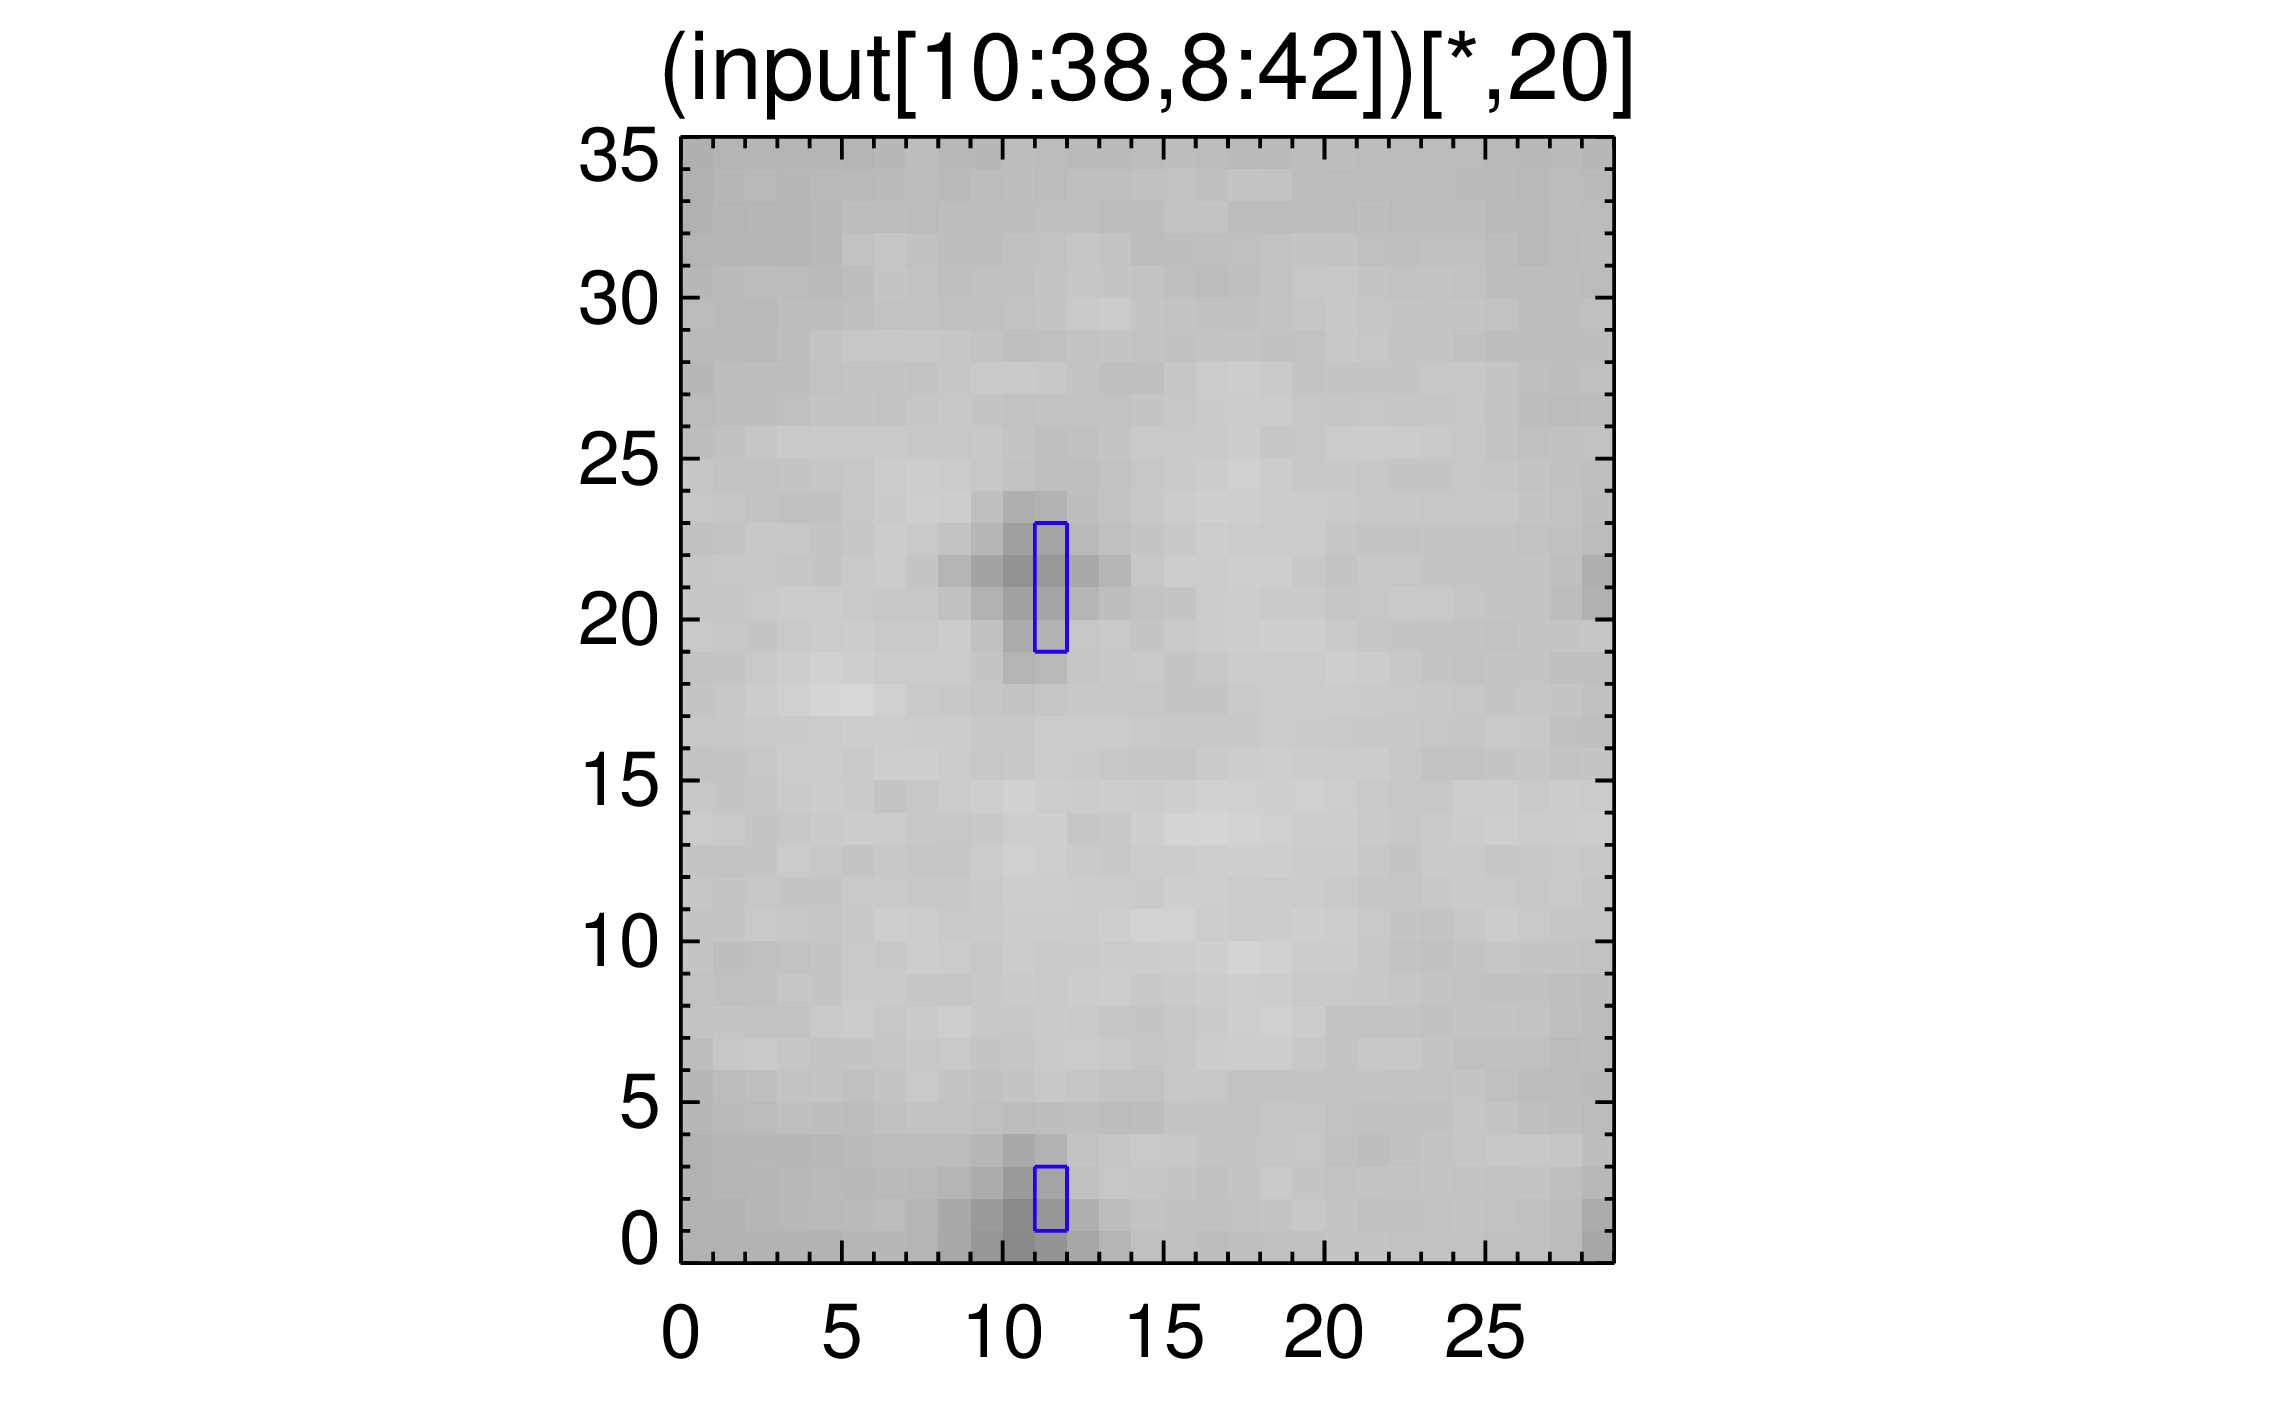
\includegraphics[width=1.3\textwidth]{../plots_tables_images/fidcheck_withembosstruncate0.png}
%         \caption{Just emboss}
%     \end{subfigure}
   
%    \begin{subfigure}[b]{.45\linewidth}
%         \centering
%         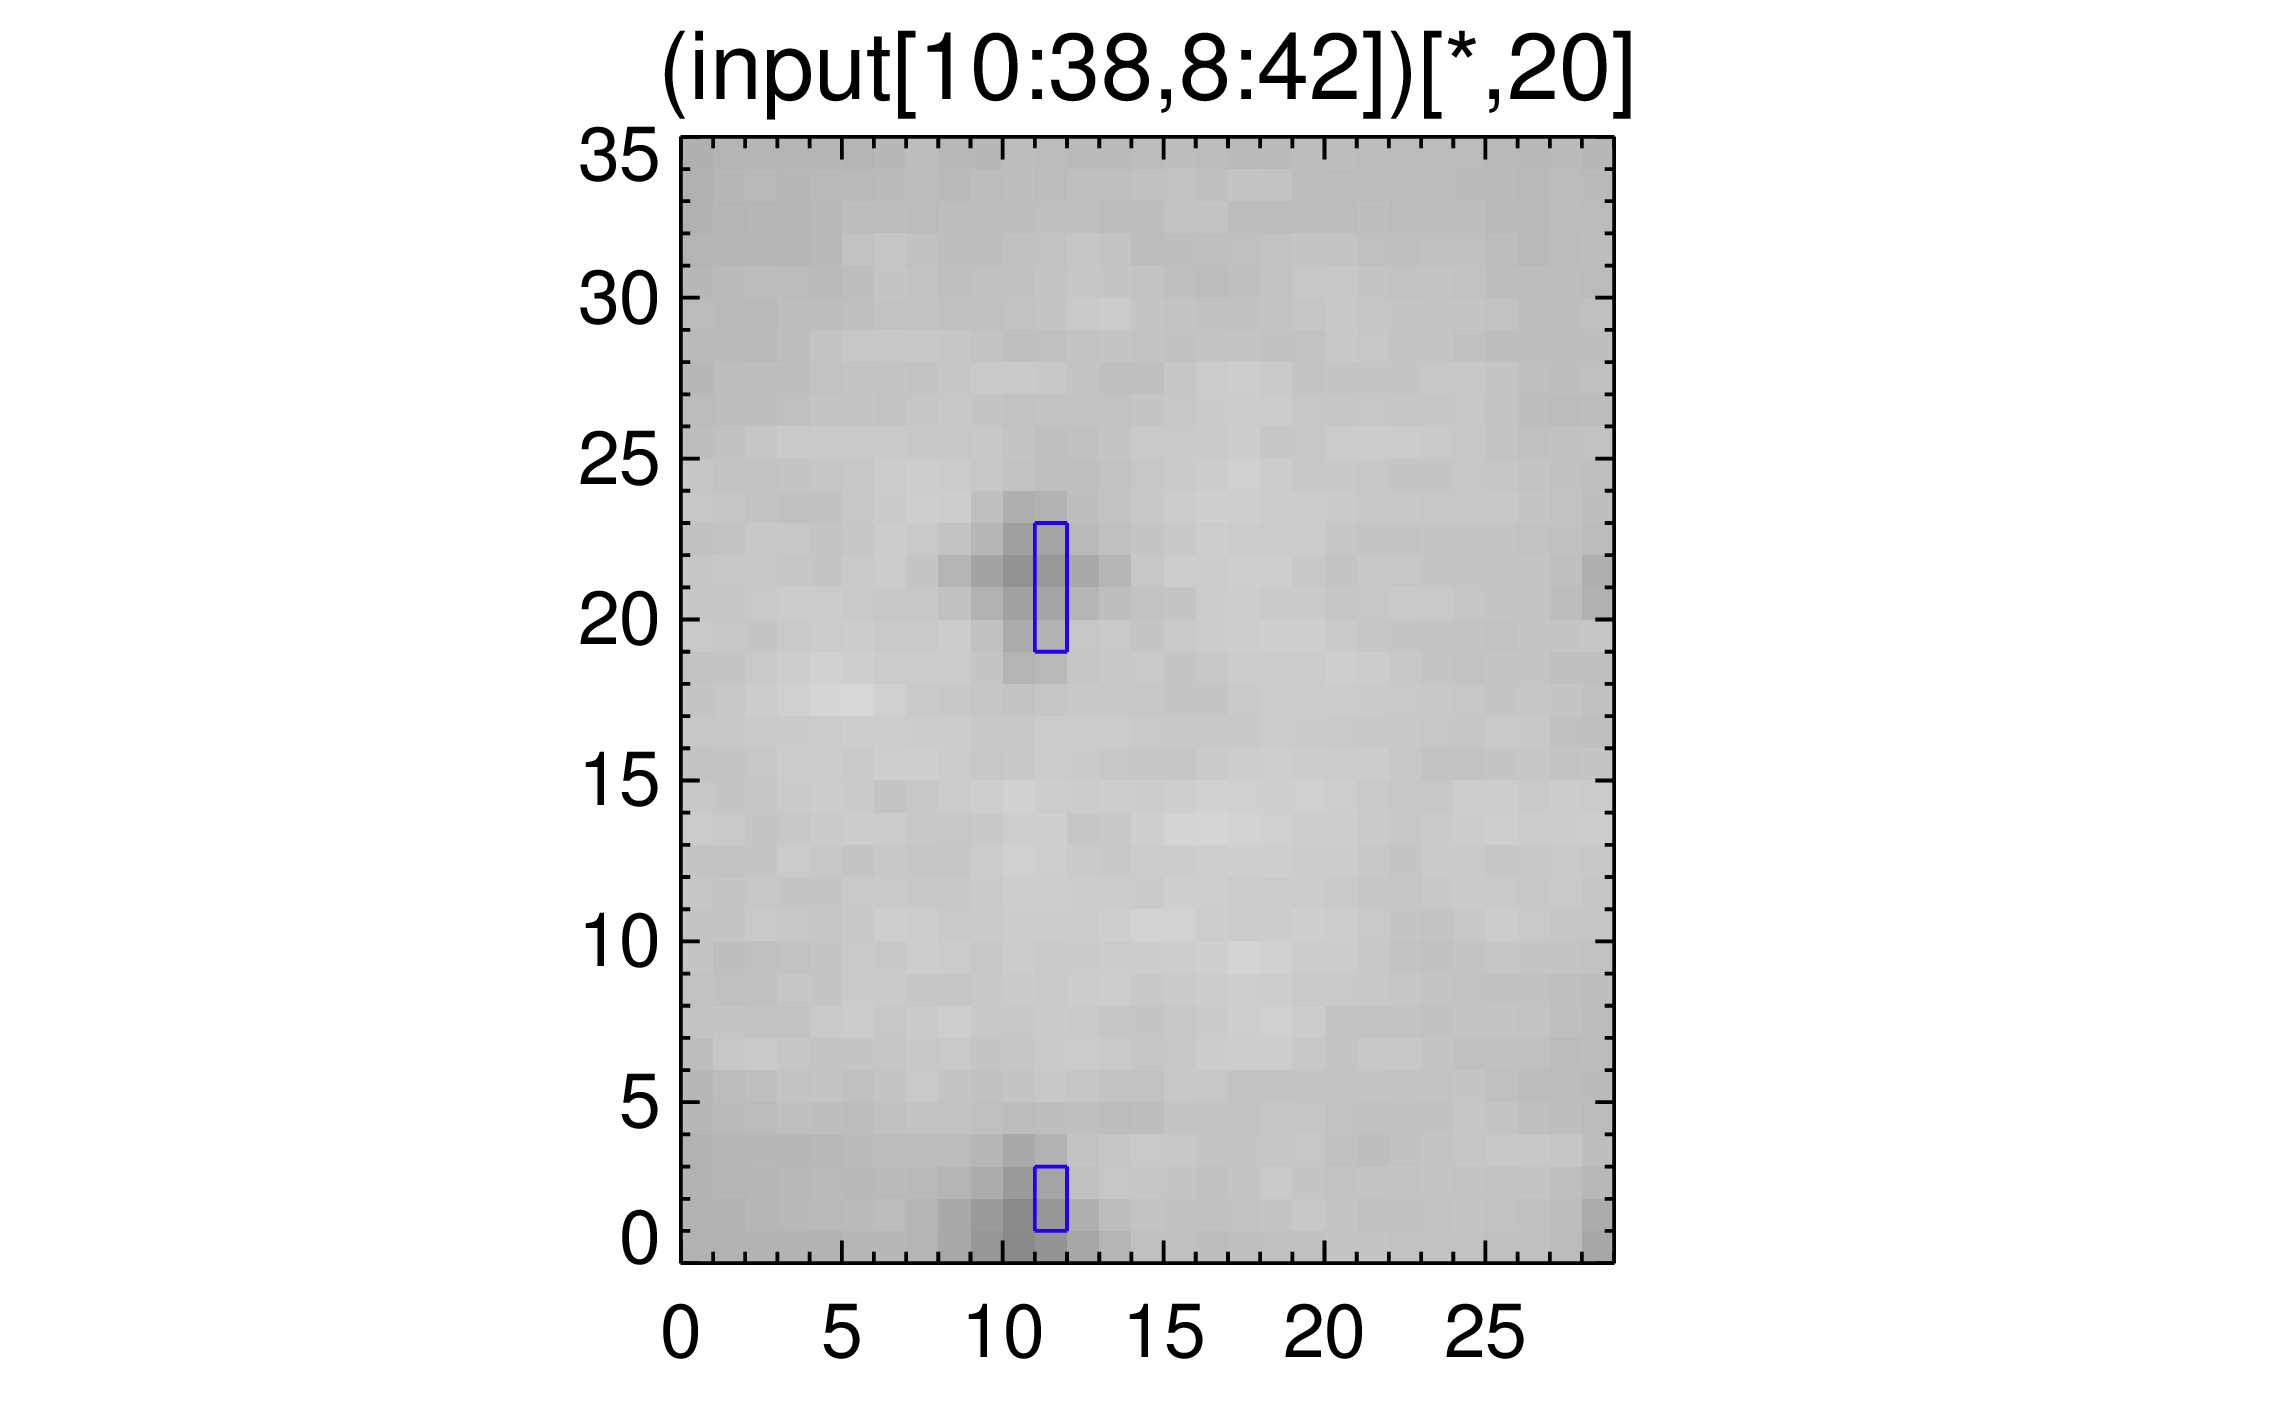
\includegraphics[width=1.3\textwidth]{../plots_tables_images/fidcheck_withshiftdifftruncate0.png}
%         \caption{Just shift\_diff}
%     \end{subfigure}
%     \begin{subfigure}[b]{.45\linewidth}
%         \centering
%         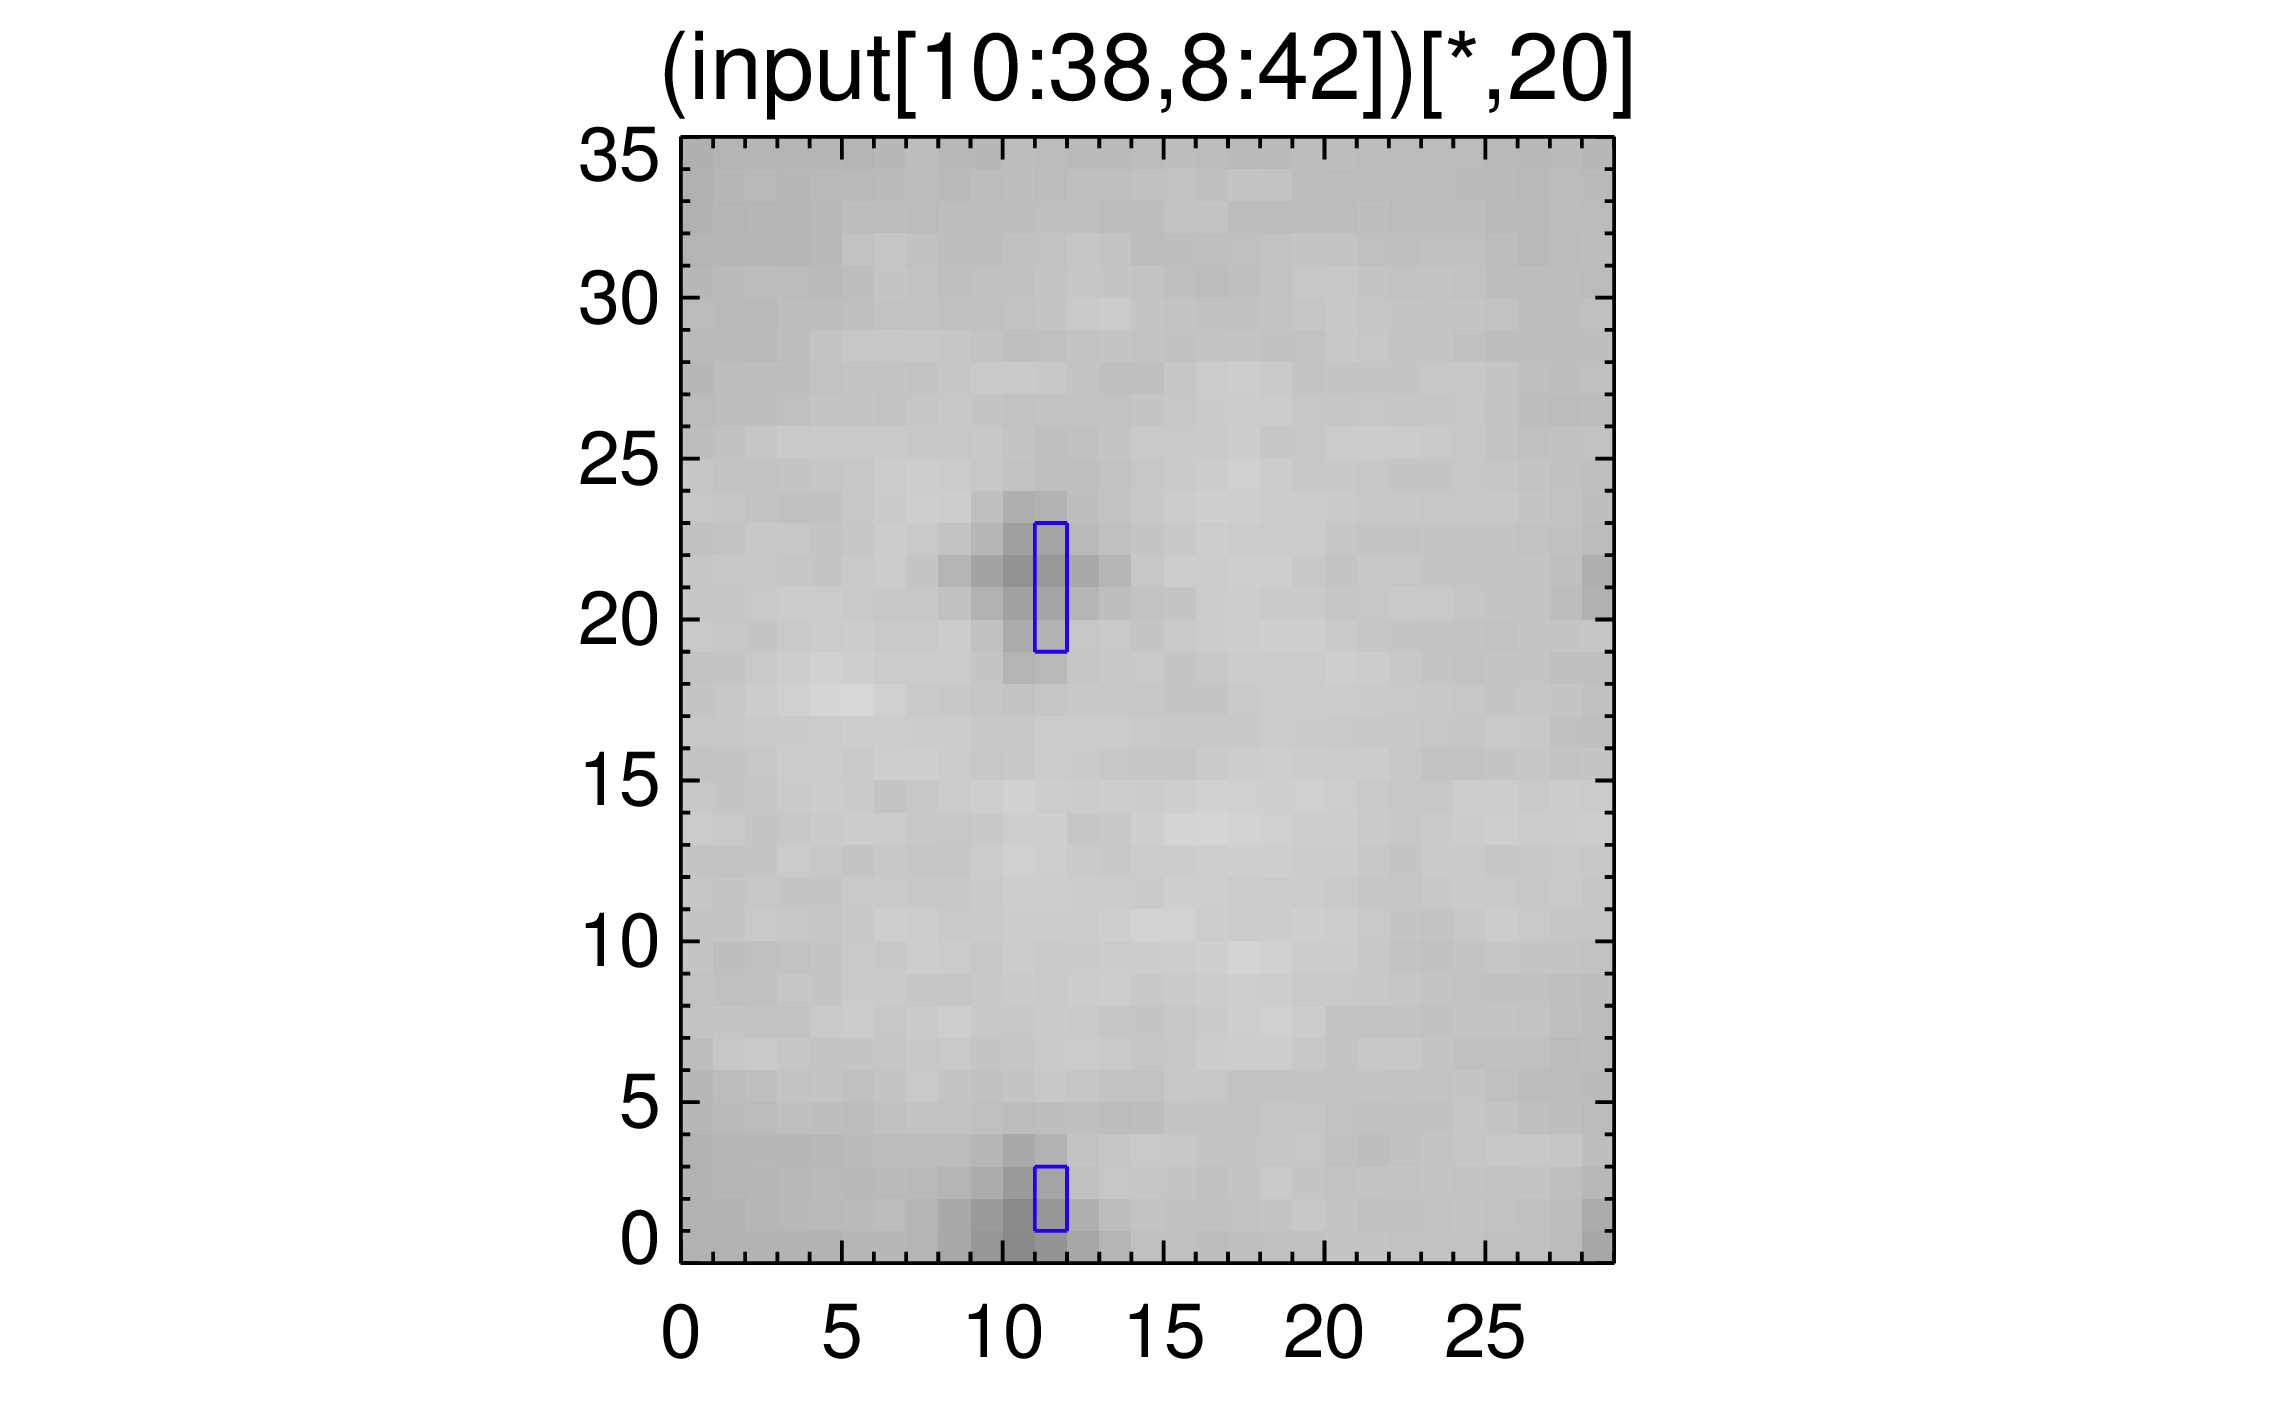
\includegraphics[width=1.3\textwidth]{../plots_tables_images/fidcheck_withnotruncate0.png}
%         \caption{No keywords}
%     \end{subfigure}
%     \caption{Only one of the images is different from the other. Can you guess which of the WHO THE WHAT NOW}
%     \label{whyedgetrunc}
% \end{figure}

\begin{figure}[!ht]
    \ffigbox[][\FBheight]{%
    \begin{subfloatrow}[2]%
        \ffigbox[\FBwidth]%
       {%
       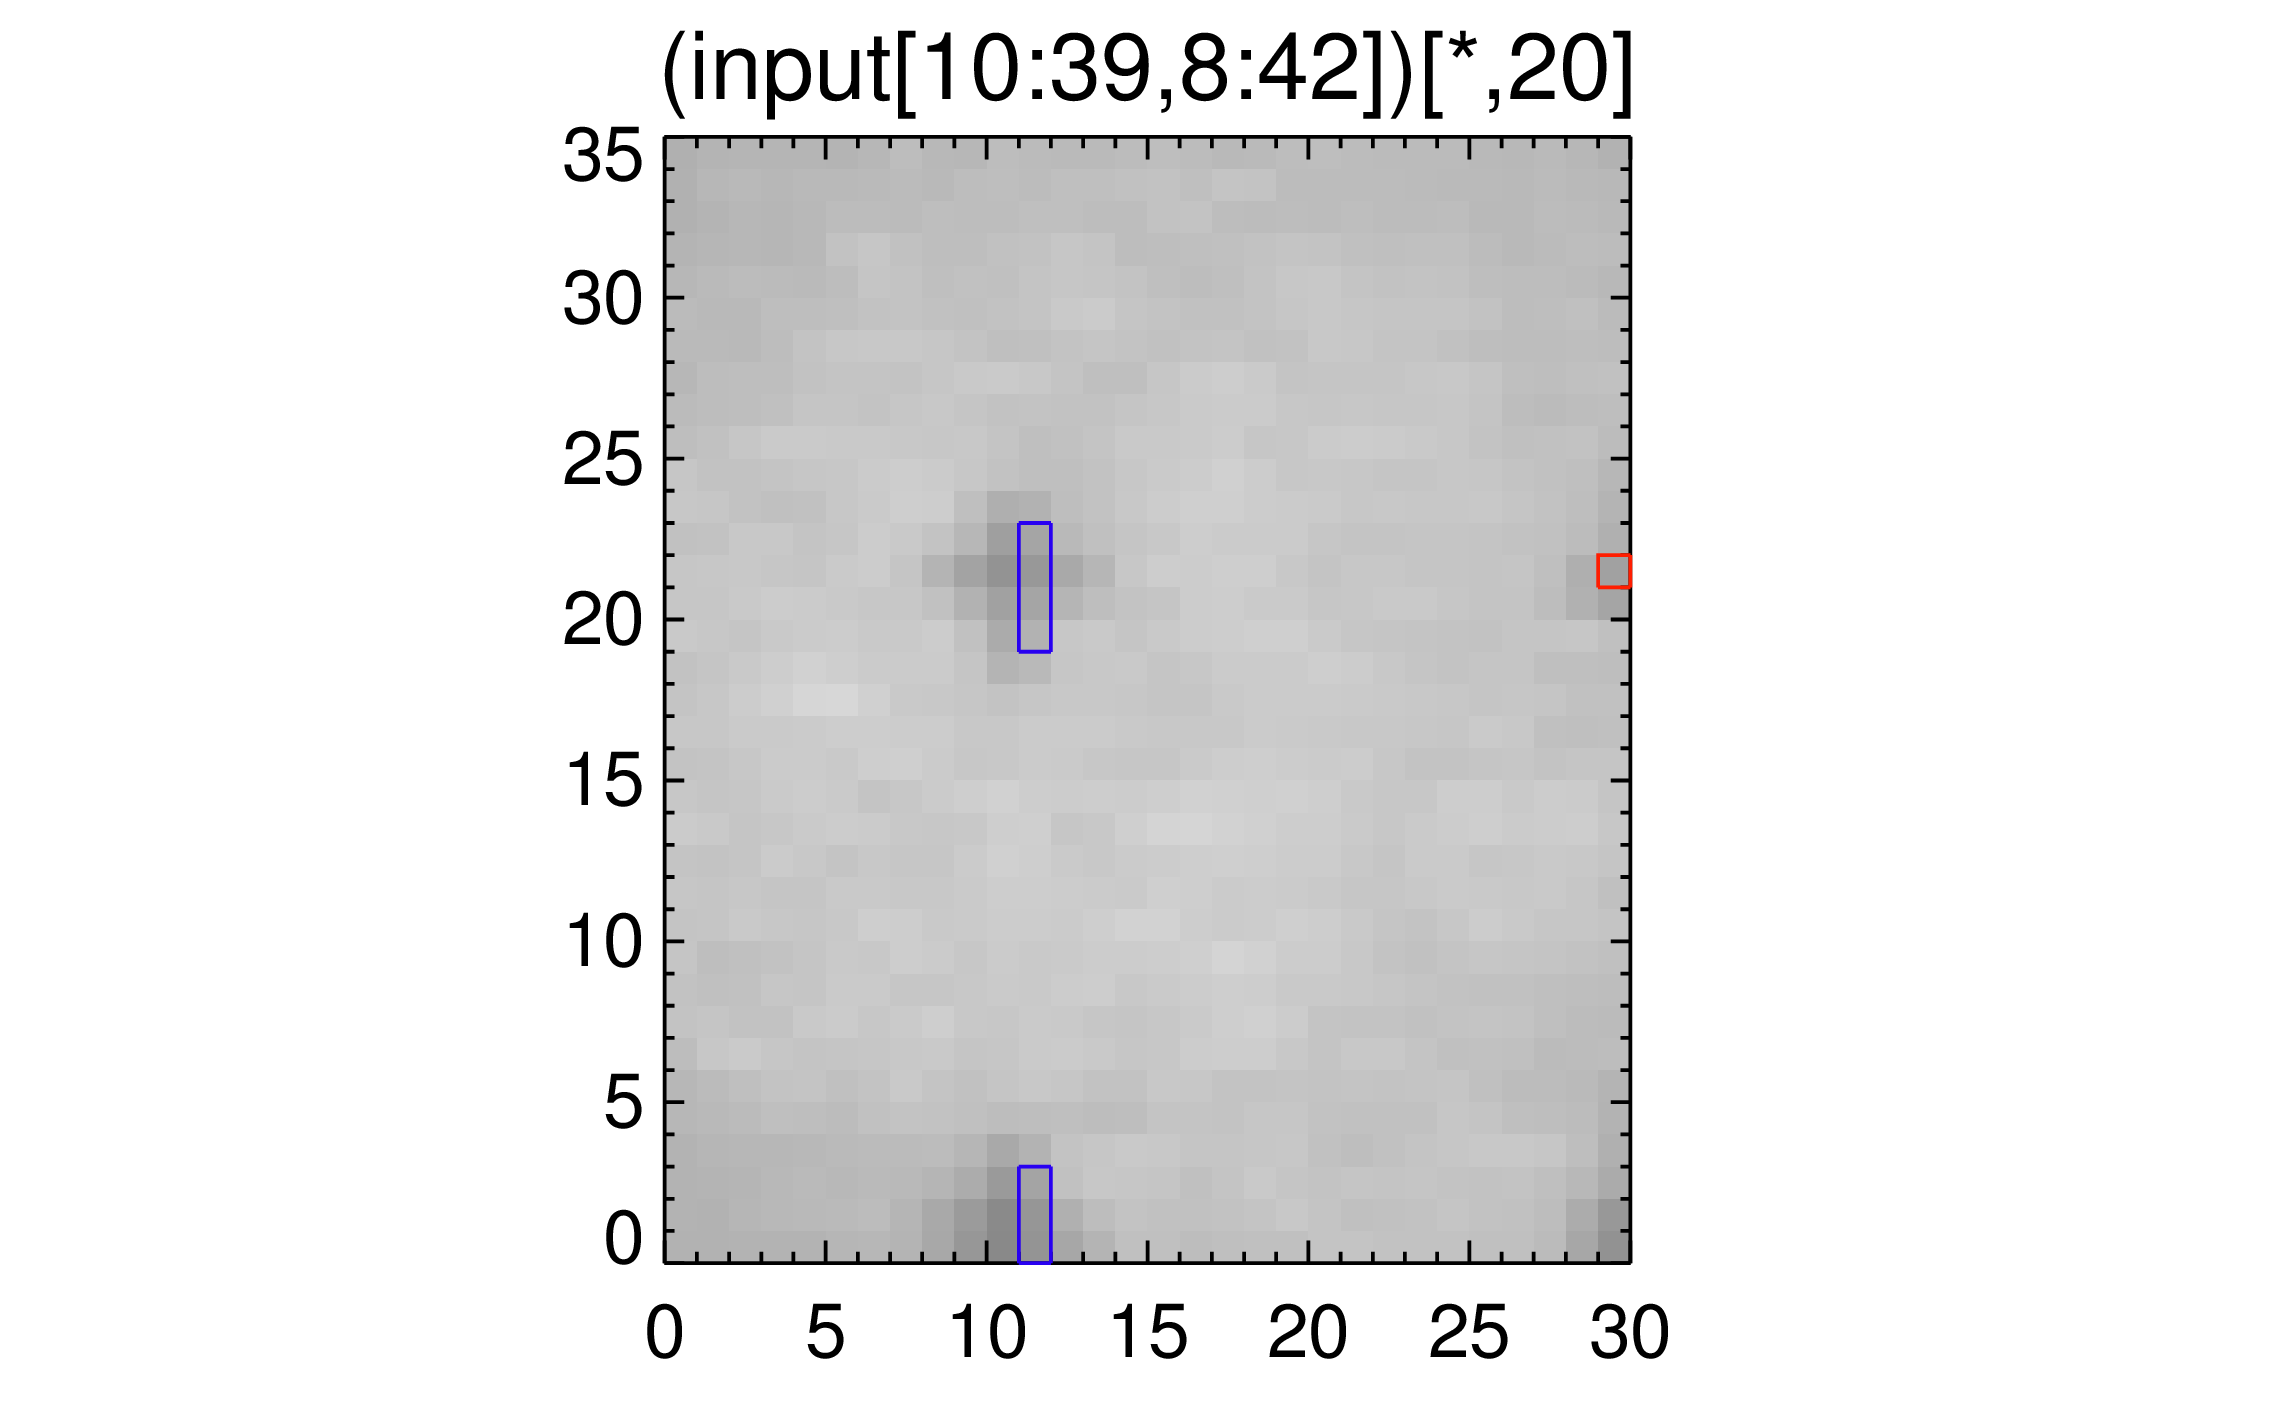
\includegraphics[width=.5\textwidth]{../plots_tables_images/fidcheck_withbothtruncate1.png}%
       }%
       {%
       \caption{Both filters have keyword}%
       }%
        \ffigbox[\Xhsize]%
       {%
       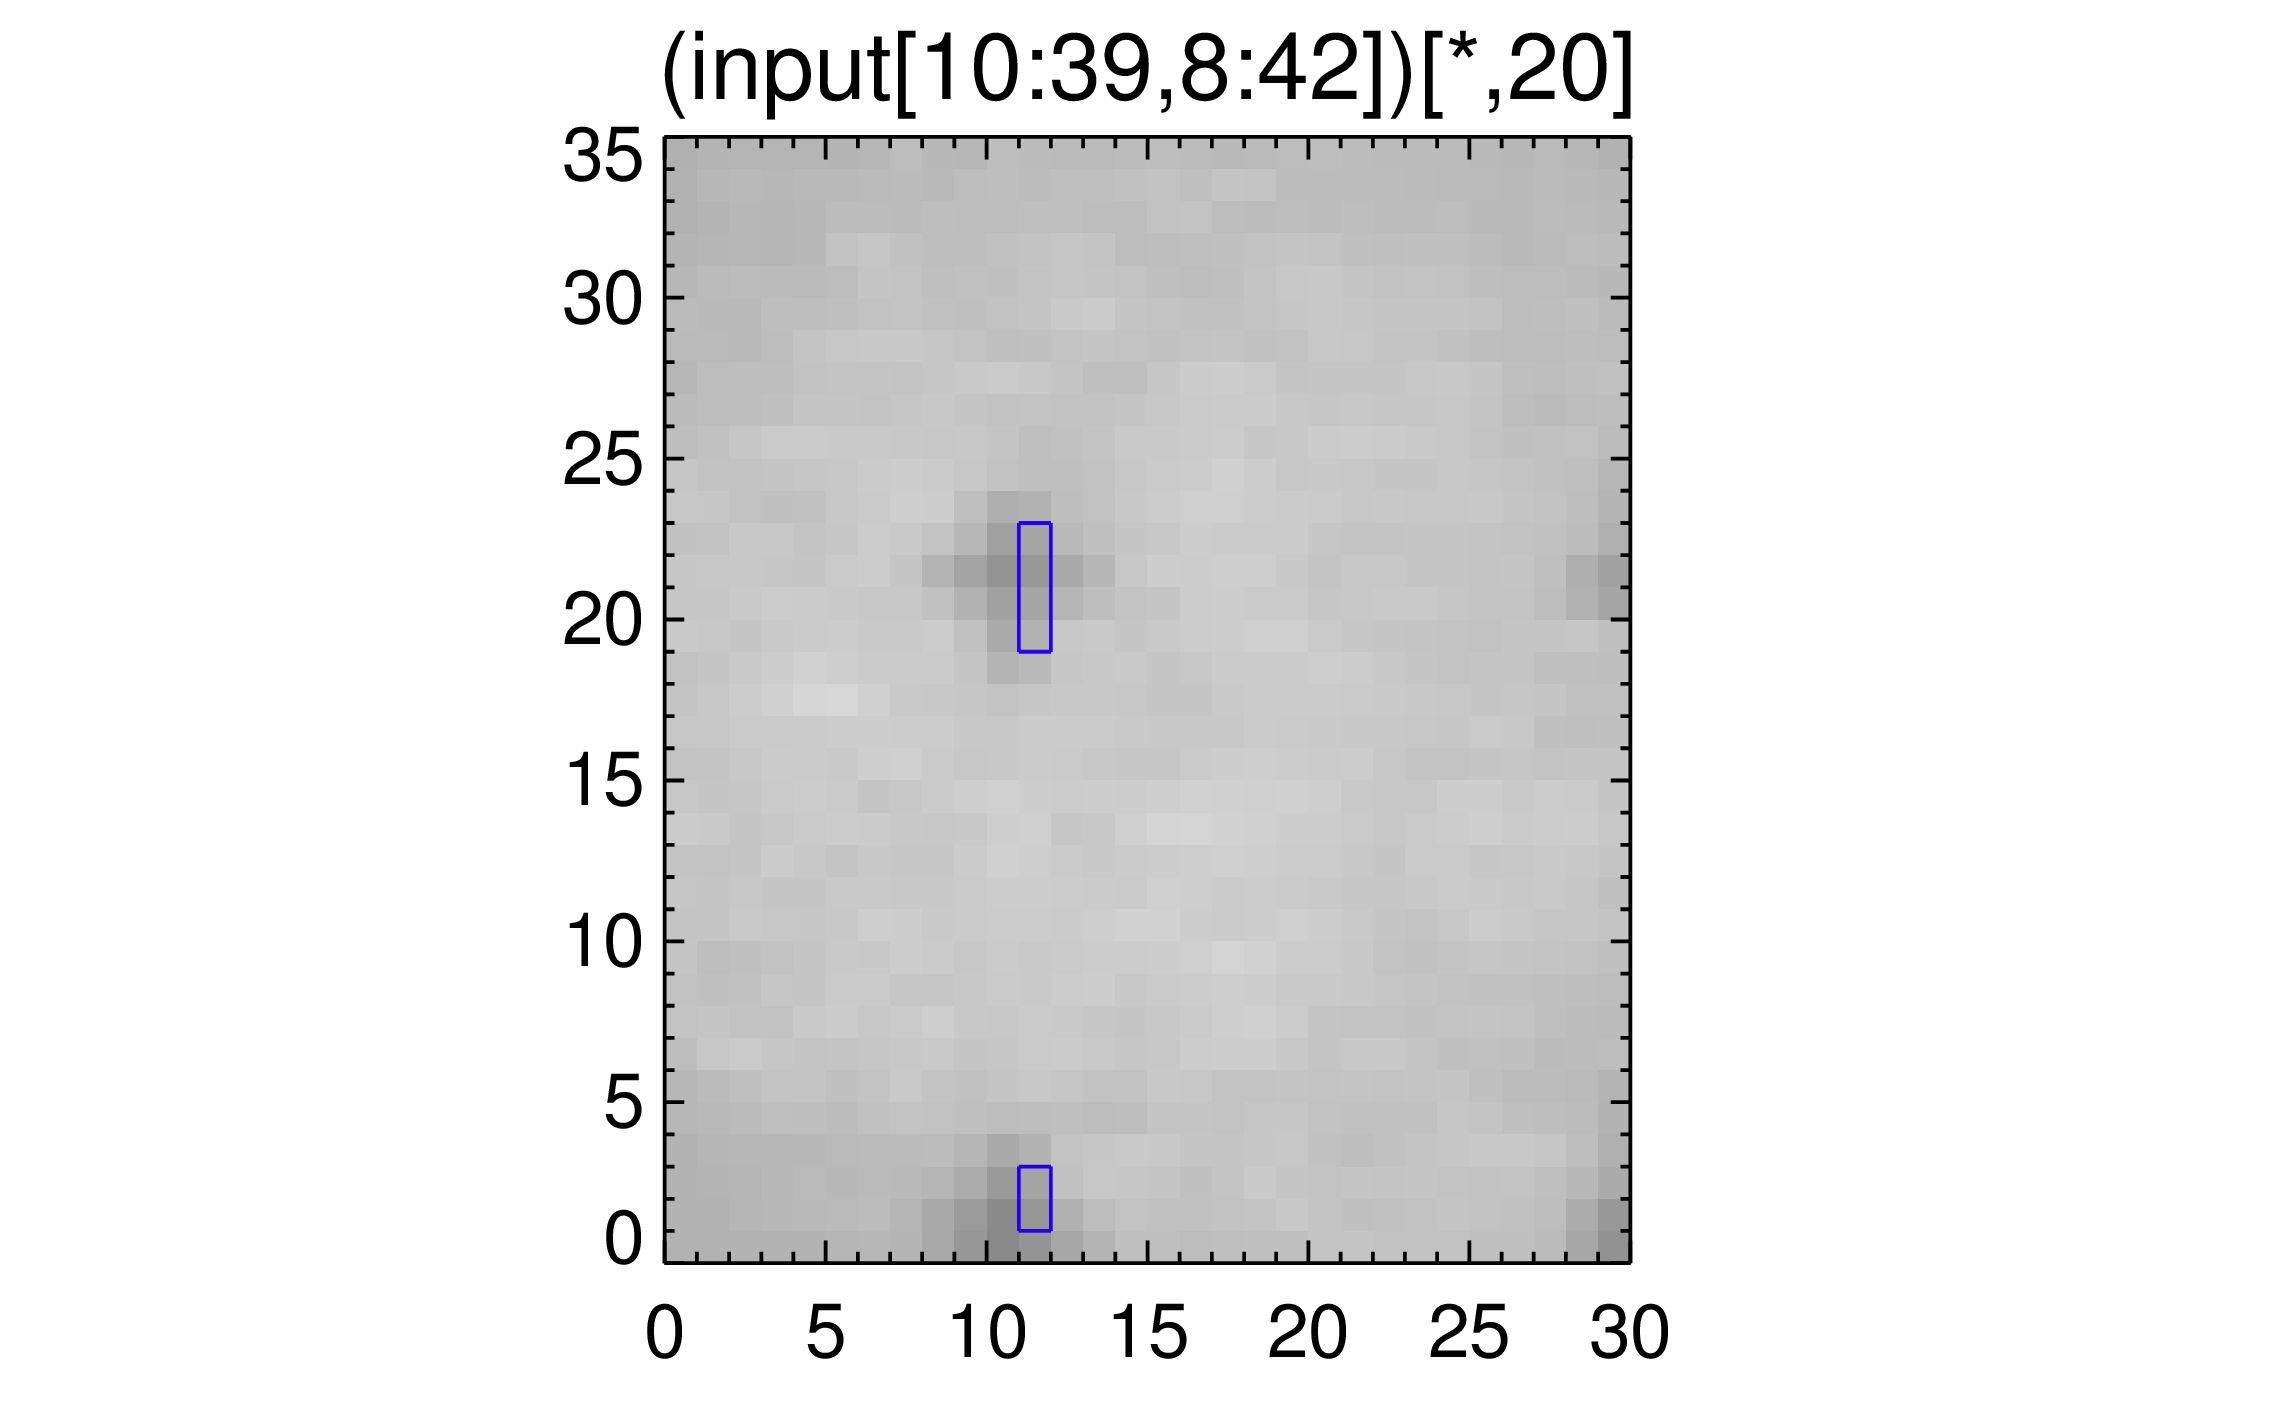
\includegraphics[width=.5\textwidth]{../plots_tables_images/fidcheck_withembosstruncate1.png}%
       }%
       {%
       \caption{Just emboss}%
       }%
    \end{subfloatrow}}

    \ffigbox[][\FBheight]{%
    \begin{subfloatrow}[2]%
        \ffigbox[\FBwidth]%
       {%
       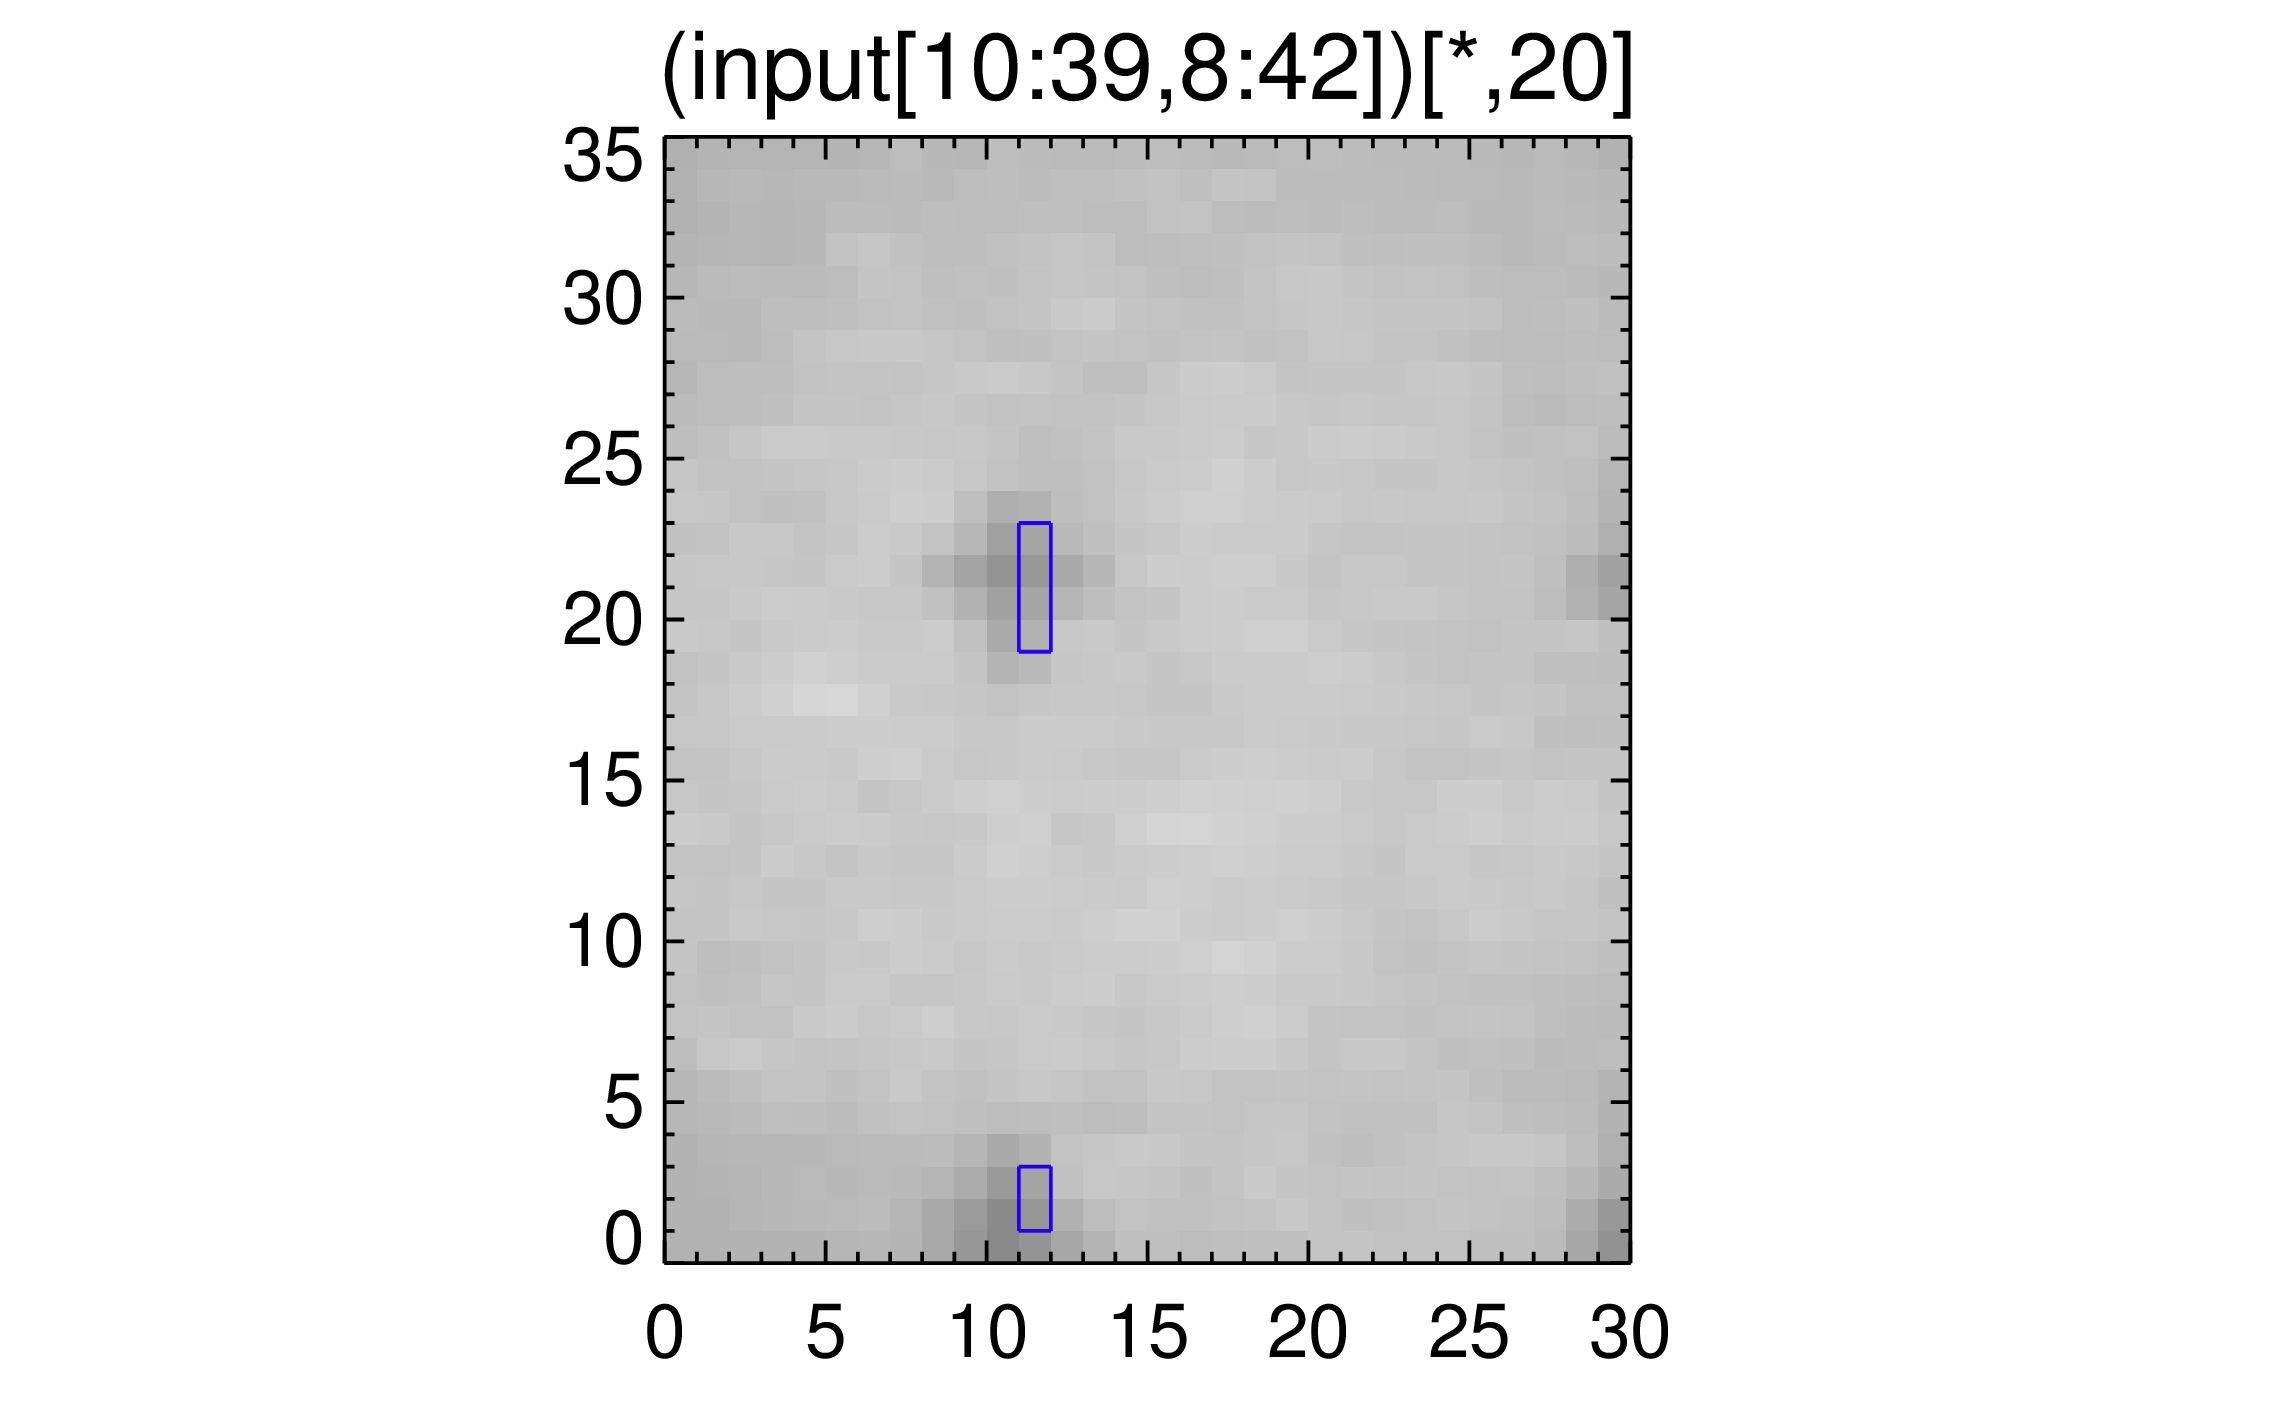
\includegraphics[width=.5\textwidth]{../plots_tables_images/fidcheck_withshiftdifftruncate1.png}%
       }%
       {%
       \caption{Just shift\_diff}%
       }%
        \ffigbox[\Xhsize]%
       {%
       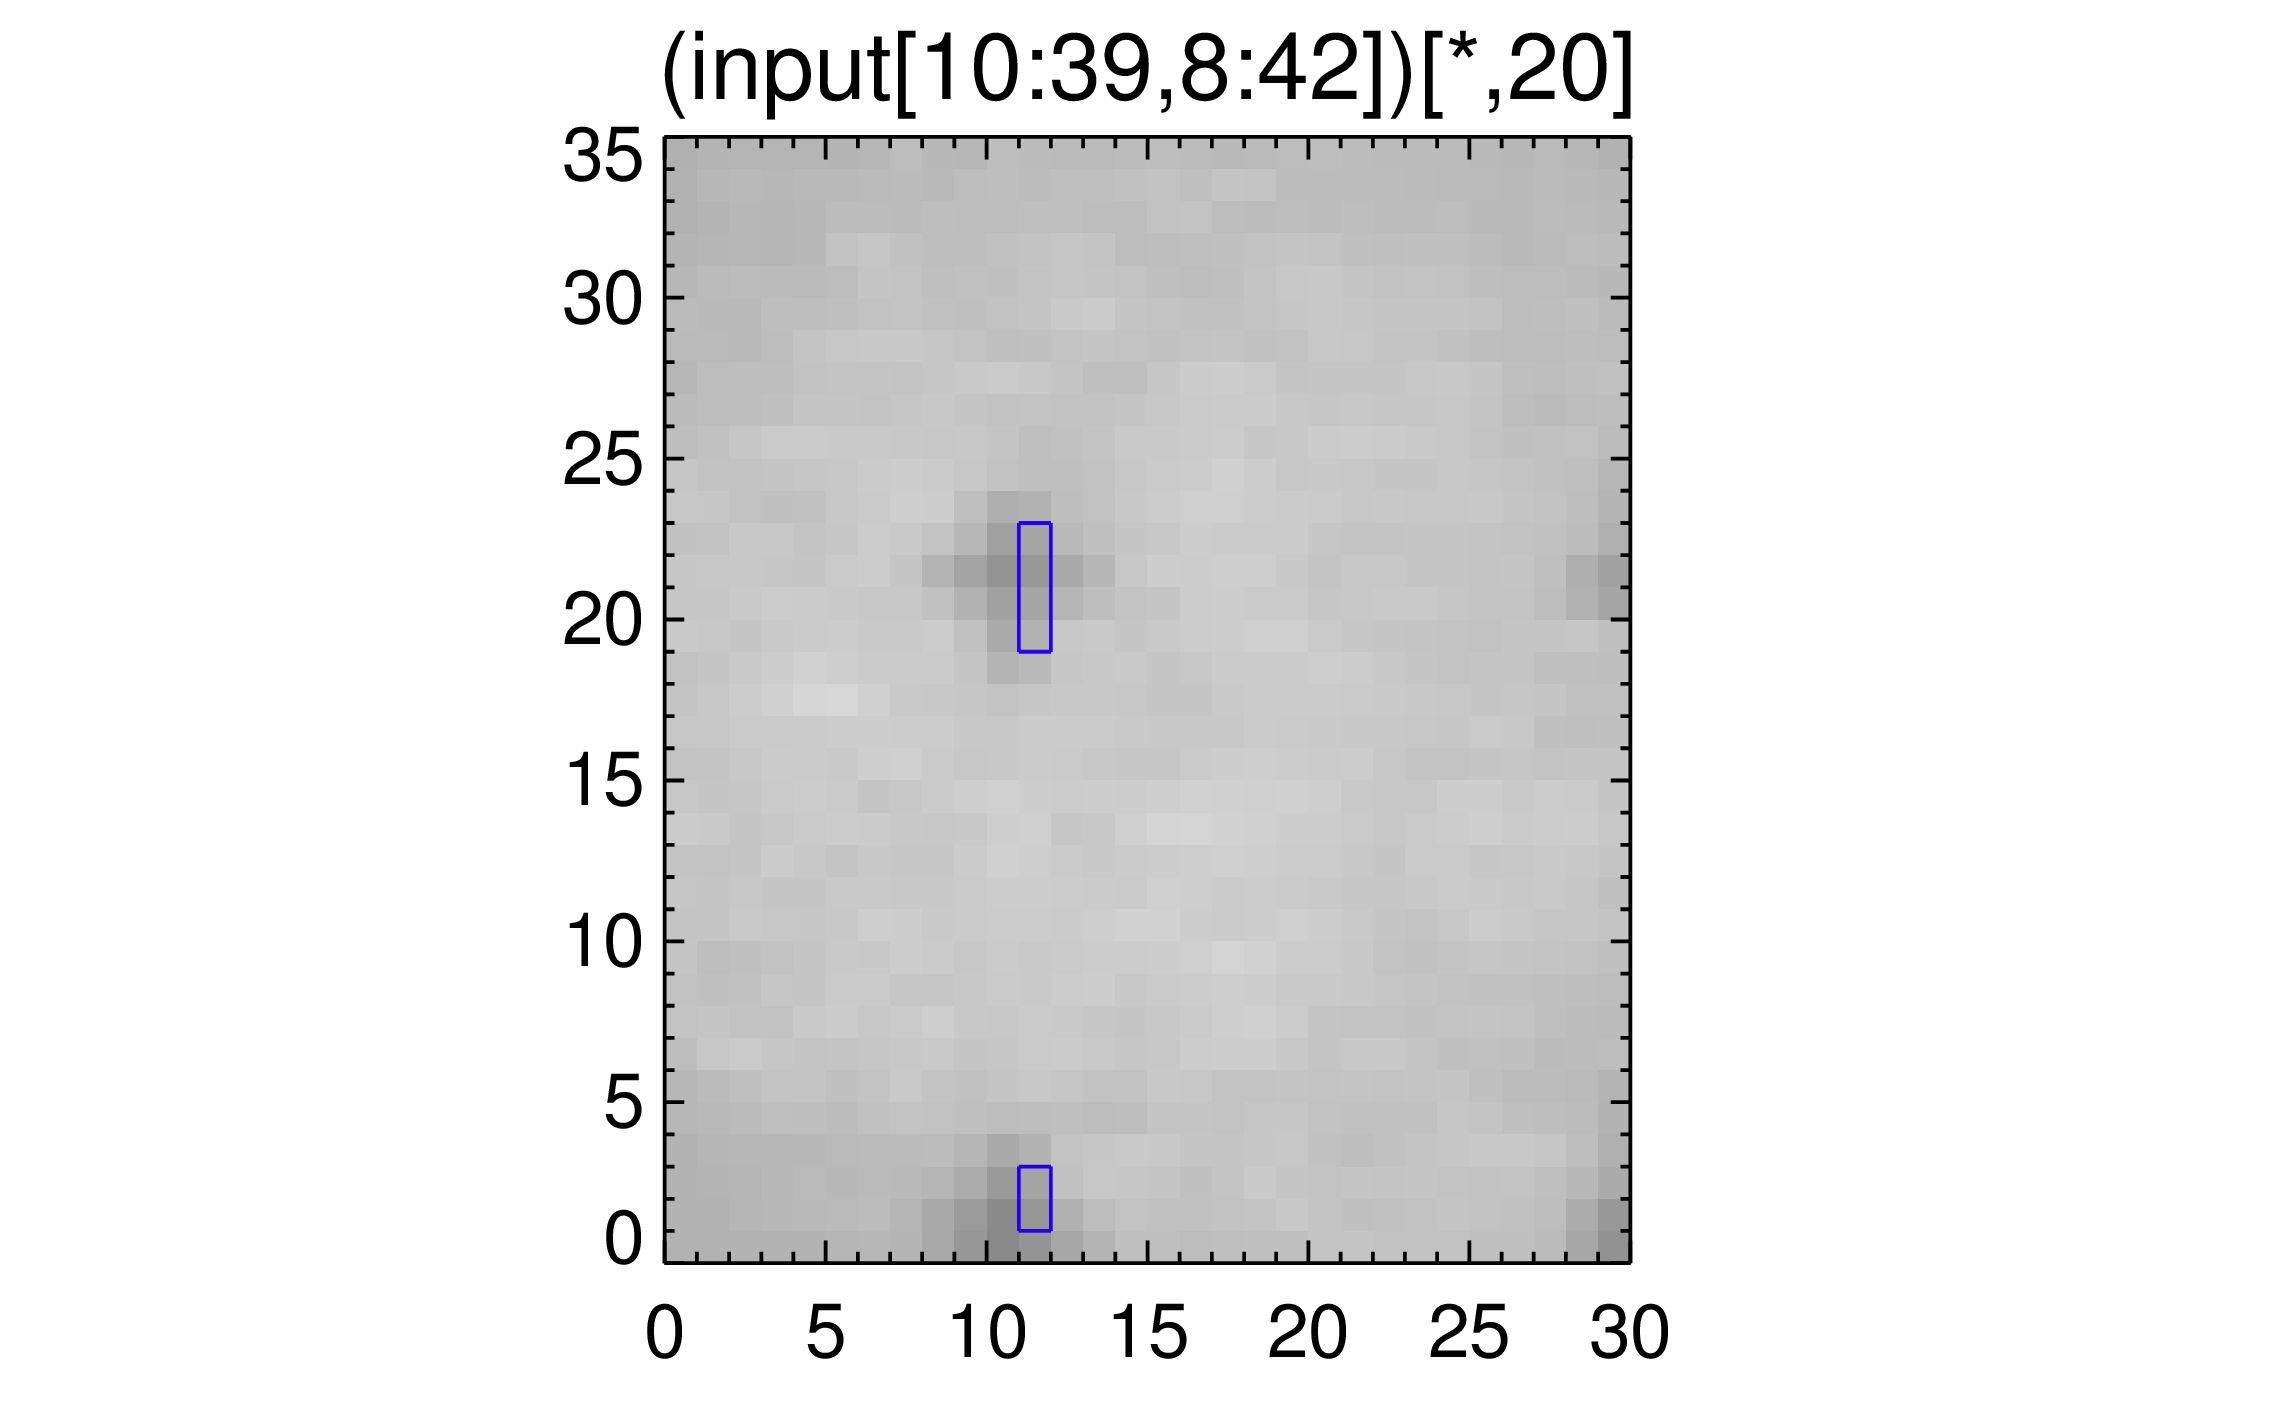
\includegraphics[width=.5\textwidth]{../plots_tables_images/fidcheck_withnotruncate1.png}%
       }%
       {%
       \caption{No keywords}%
       }%
    \end{subfloatrow}}{\caption{Another example, but this time we see that the one with both keyword sets has found a row that we can work with.}\label{whystopnow}}
\end{figure}

% \begin{figure}[!h]
%     \centering 
%     \begin{subfigure}[b]{.45\linewidth}
%         \centering
%         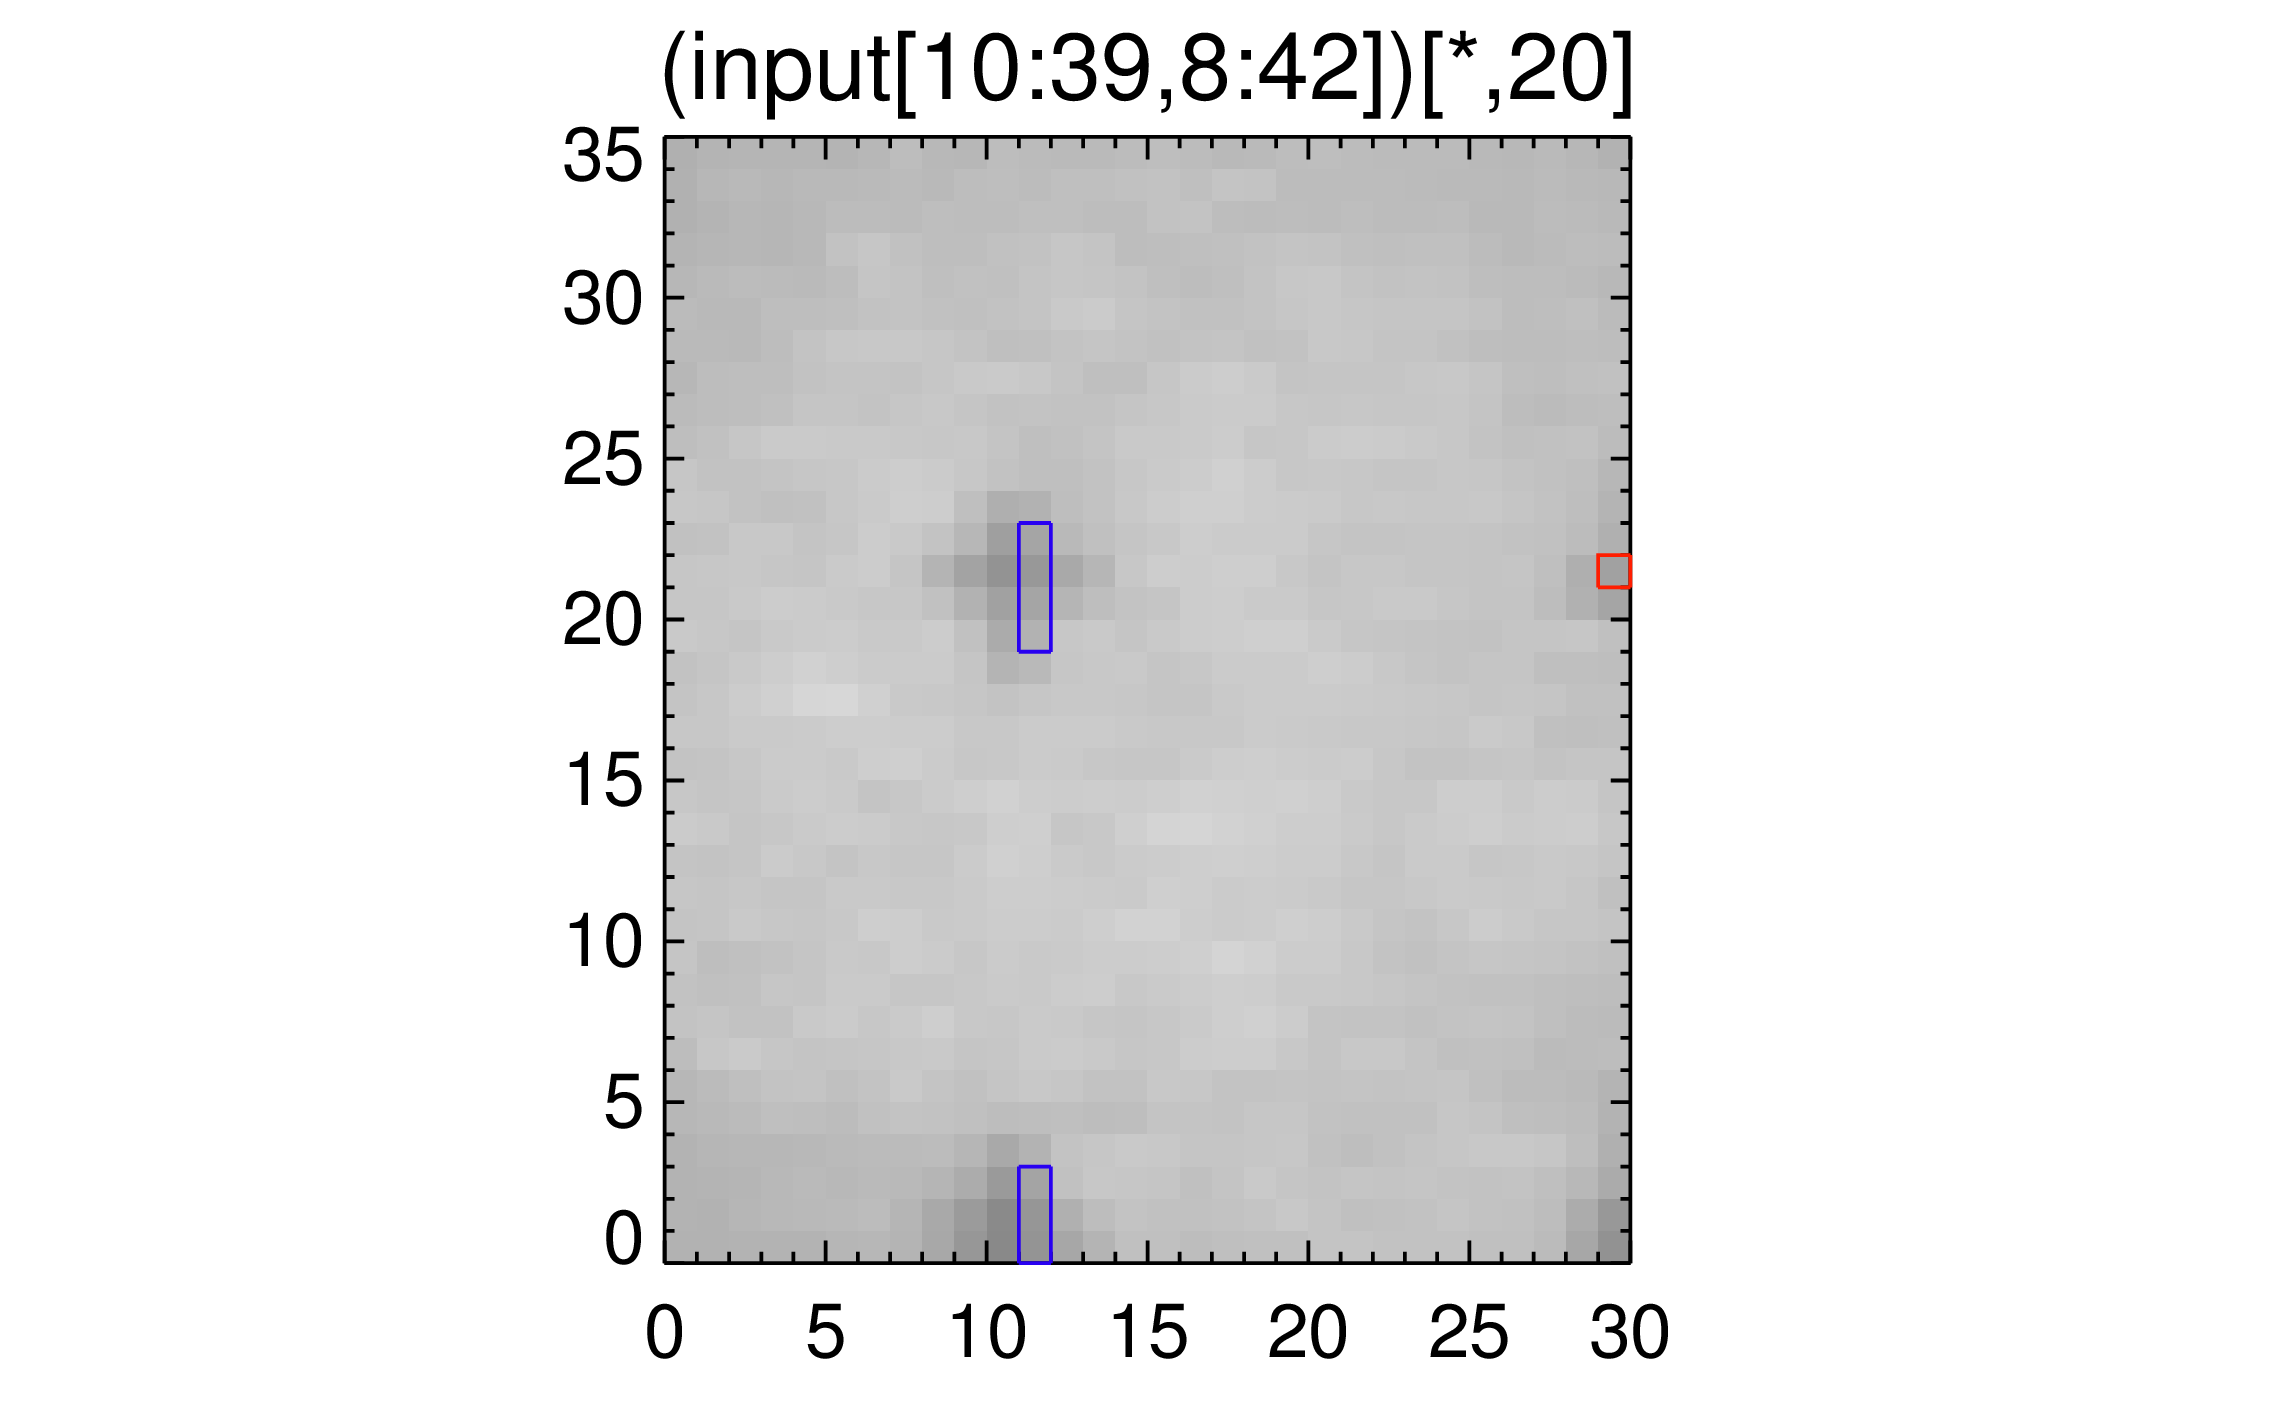
\includegraphics[width=1.3\textwidth]{../plots_tables_images/fidcheck_withbothtruncate1.png}
%         \caption{Both filters have keyword}
%     \end{subfigure}
%     \begin{subfigure}[b]{.45\linewidth}
%         \centering
%         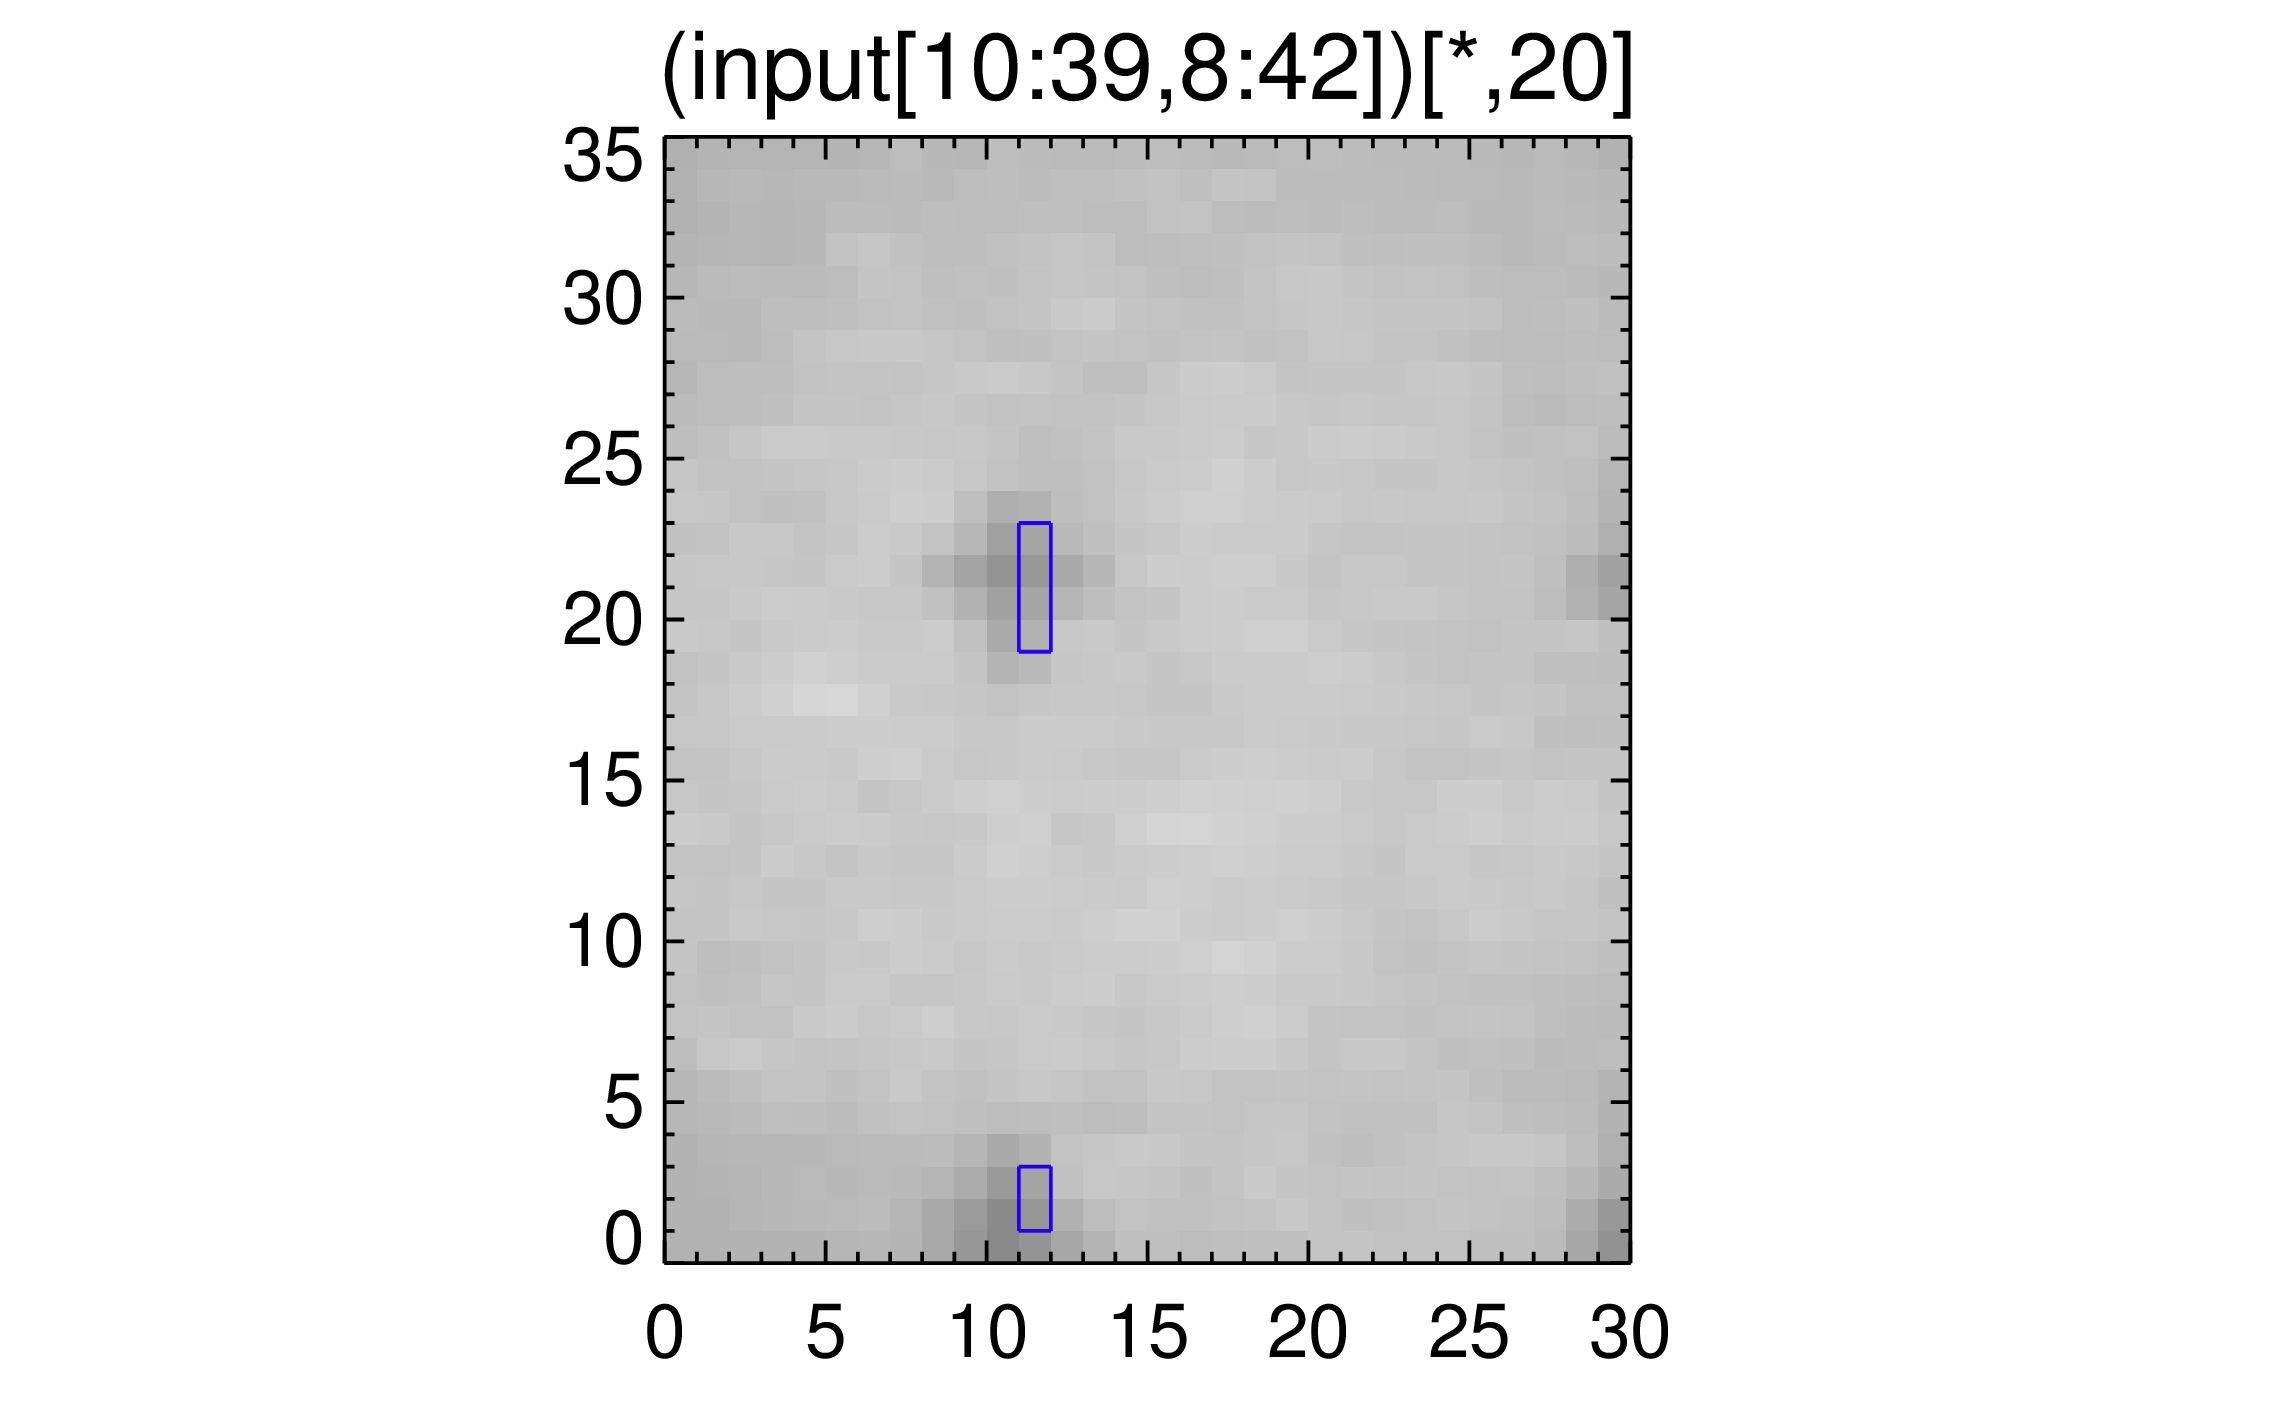
\includegraphics[width=1.3\textwidth]{../plots_tables_images/fidcheck_withembosstruncate1.png}
%         \caption{Just emboss}
%     \end{subfigure}
   
%    \begin{subfigure}[b]{.45\linewidth}
%         \centering
%         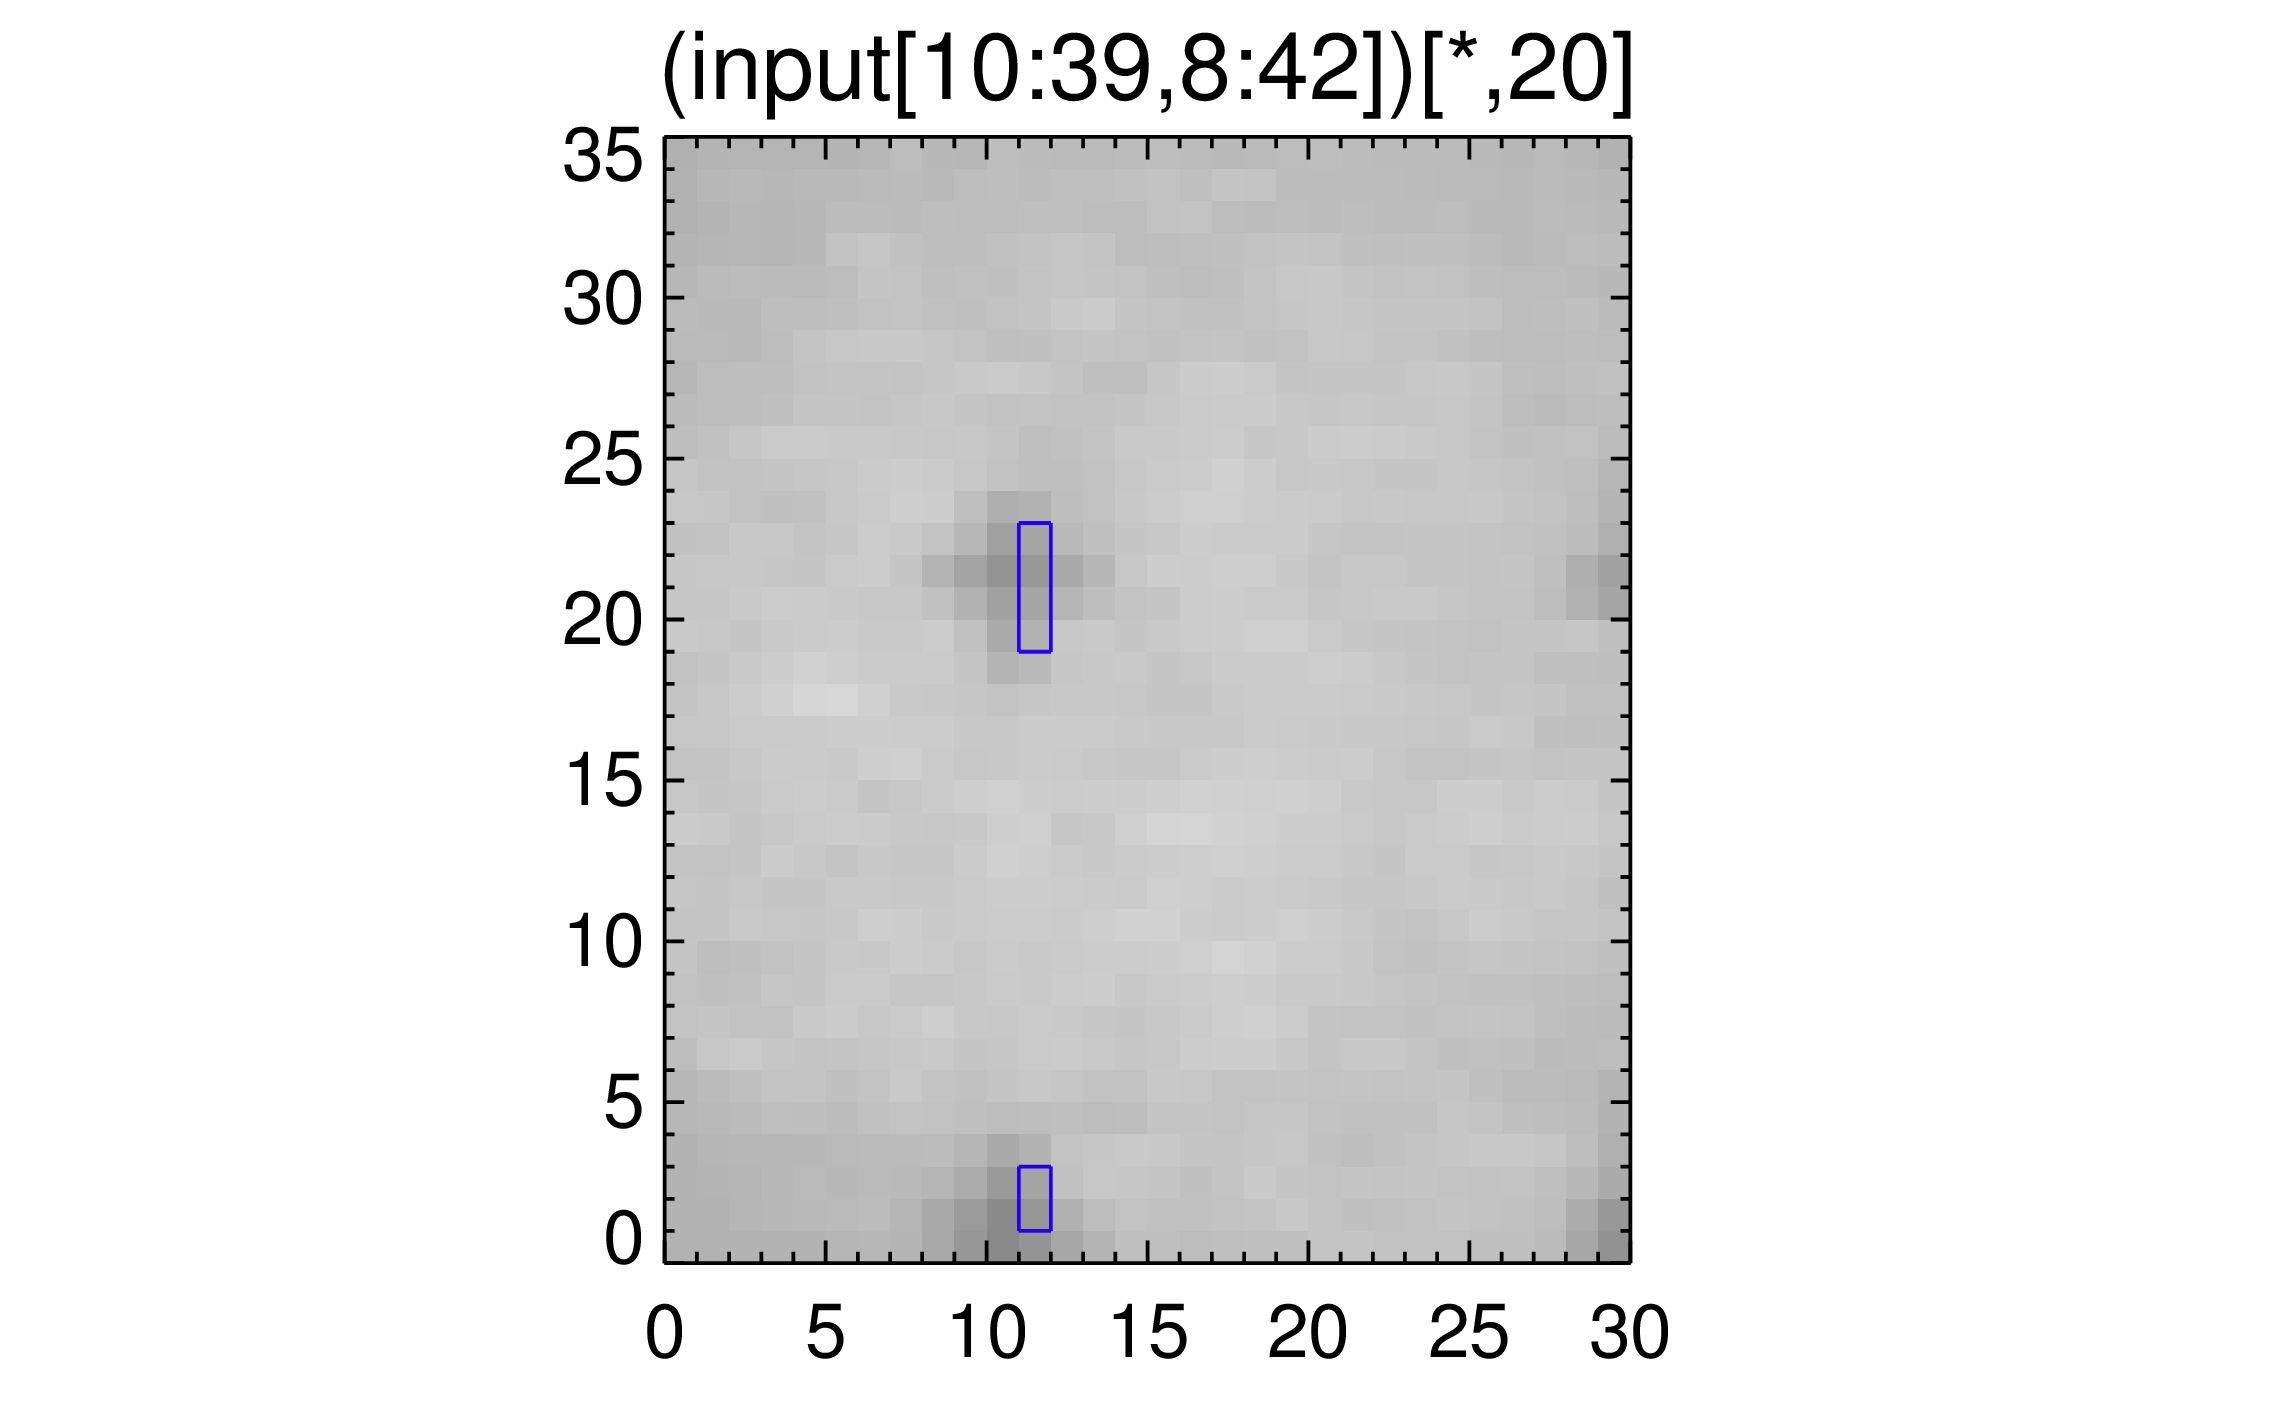
\includegraphics[width=1.3\textwidth]{../plots_tables_images/fidcheck_withshiftdifftruncate1.png}
%         \caption{Just shift\_diff}
%     \end{subfigure}
%     \begin{subfigure}[b]{.45\linewidth}
%         \centering
%         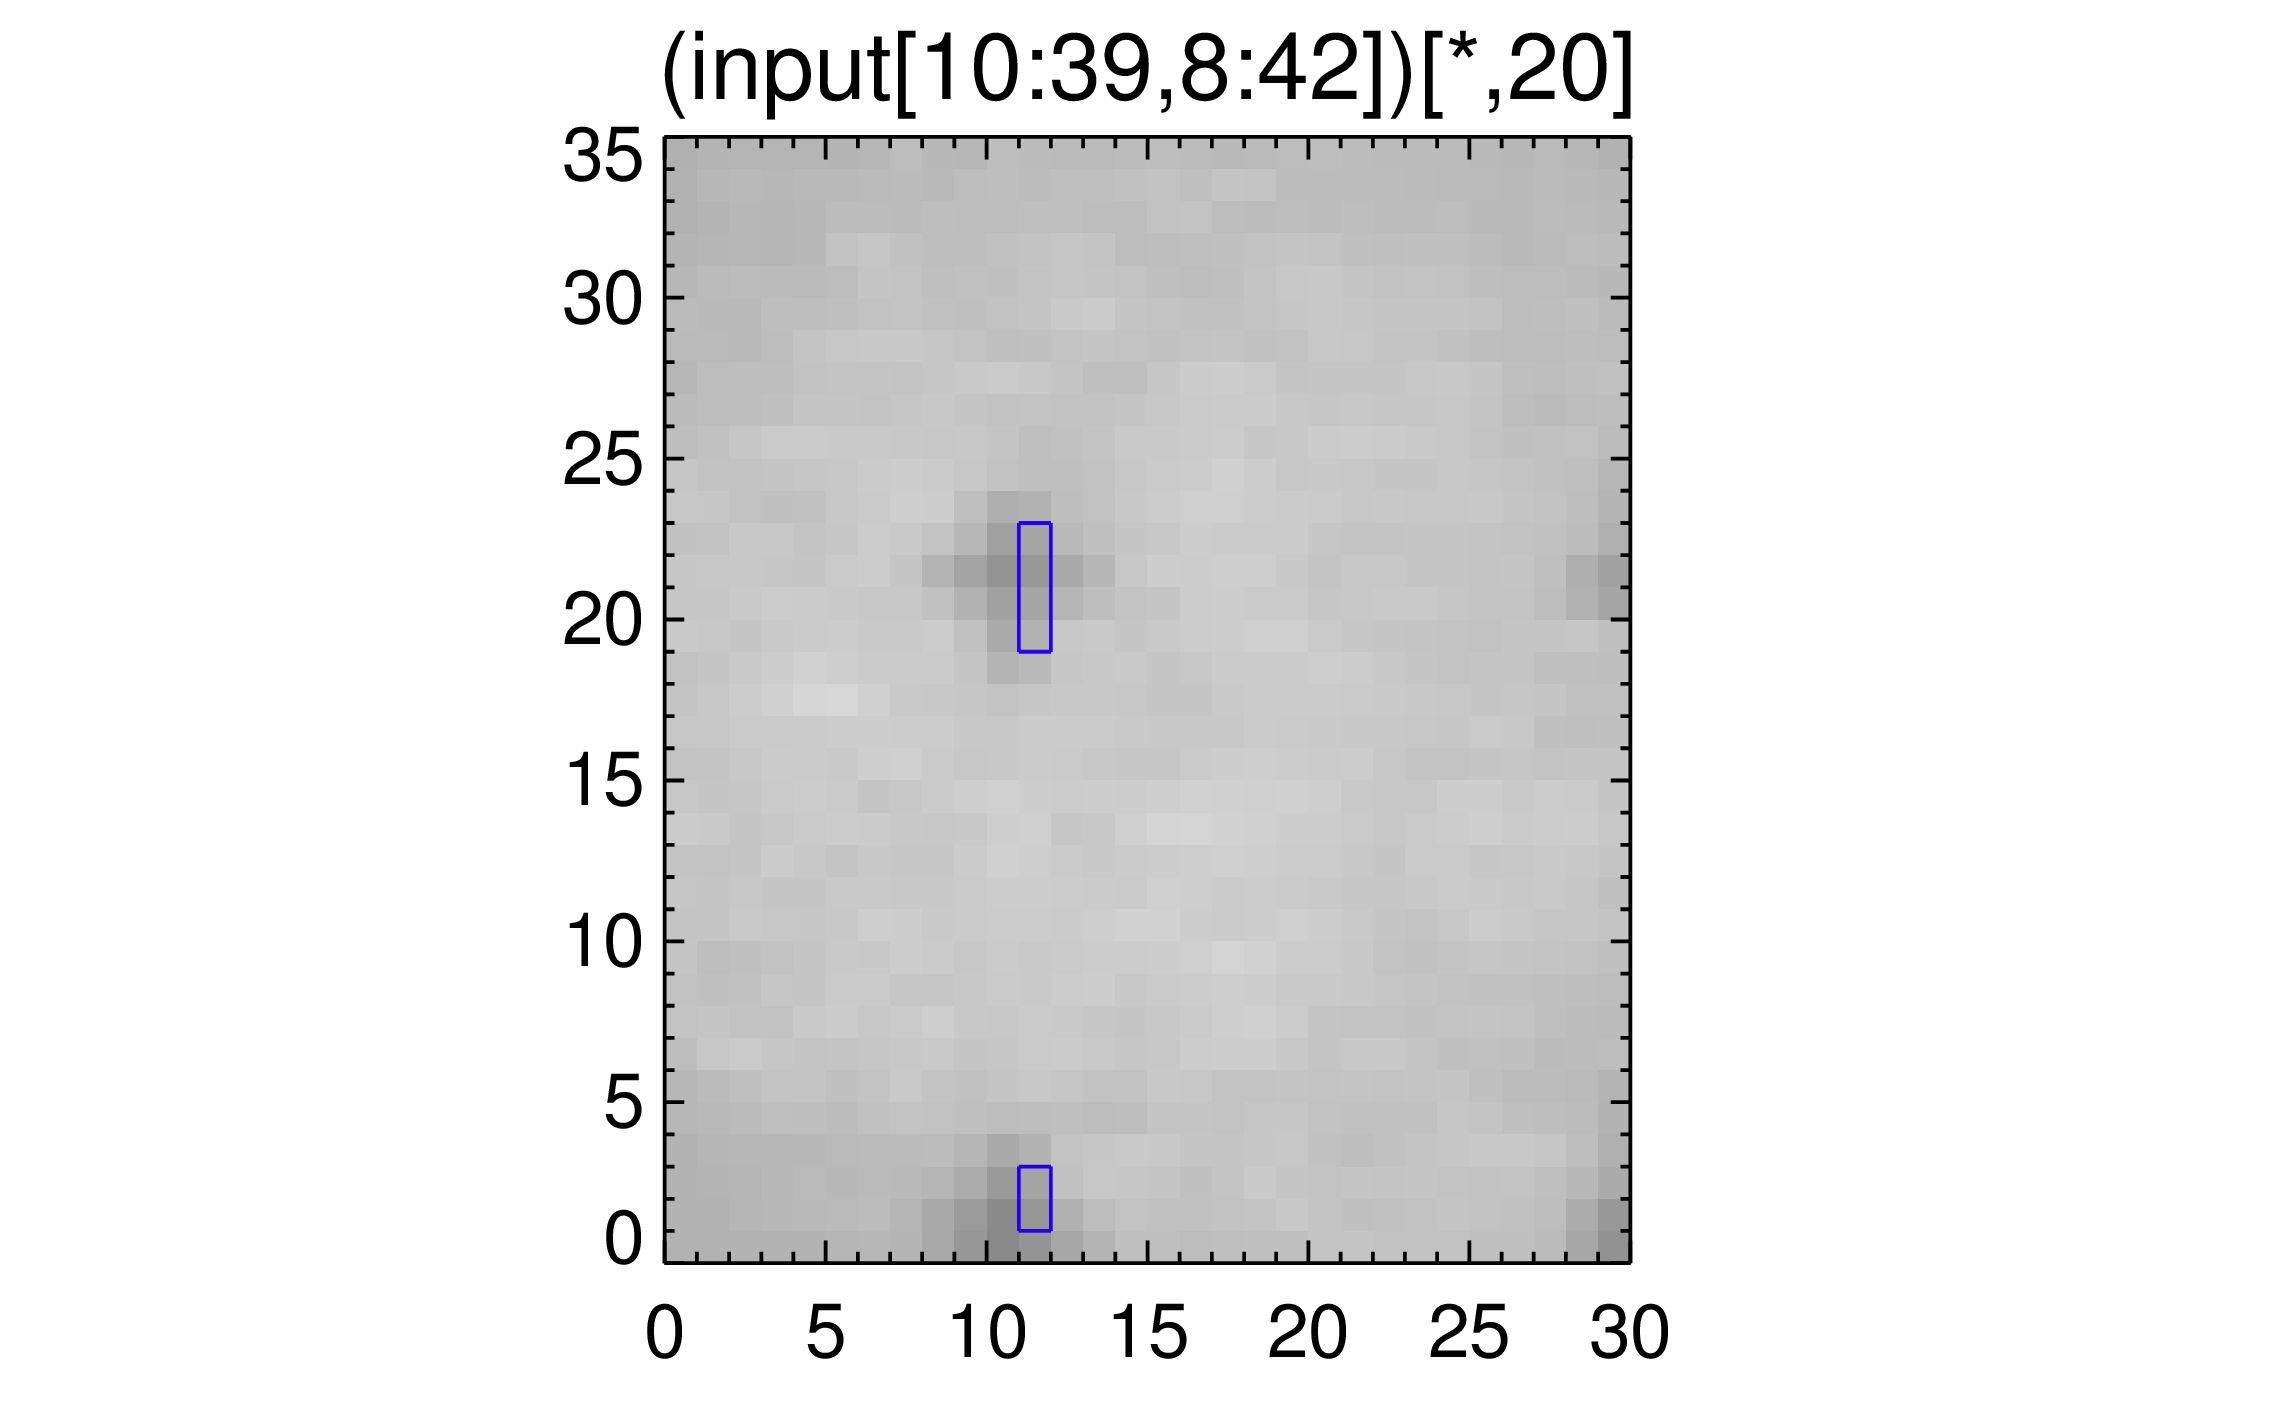
\includegraphics[width=1.3\textwidth]{../plots_tables_images/fidcheck_withnotruncate1.png}
%         \caption{No keywords}
%     \end{subfigure}
%     \caption{Another example, but this time we see that the one with both keyword sets has found a row that we can work with.}
%     \label{whystopnow}
% \end{figure}

Figure \ref{whystopnow} shows us that there are significant benefits of using the keyword \hl{\texttt{edge\_truncate}} on both filters.
% subsection edge_truncate (end)

\subsection{Another example of filters on an increasingly cropped image} % (fold)
\label{sub:another_example_of_filters_on_an_increasingly_cropped_image}

\begin{figure}[!ht]
    \ffigbox[][\FBheight]{%
    \begin{subfloatrow}[2]%
        \ffigbox[\FBwidth]%
       {%
       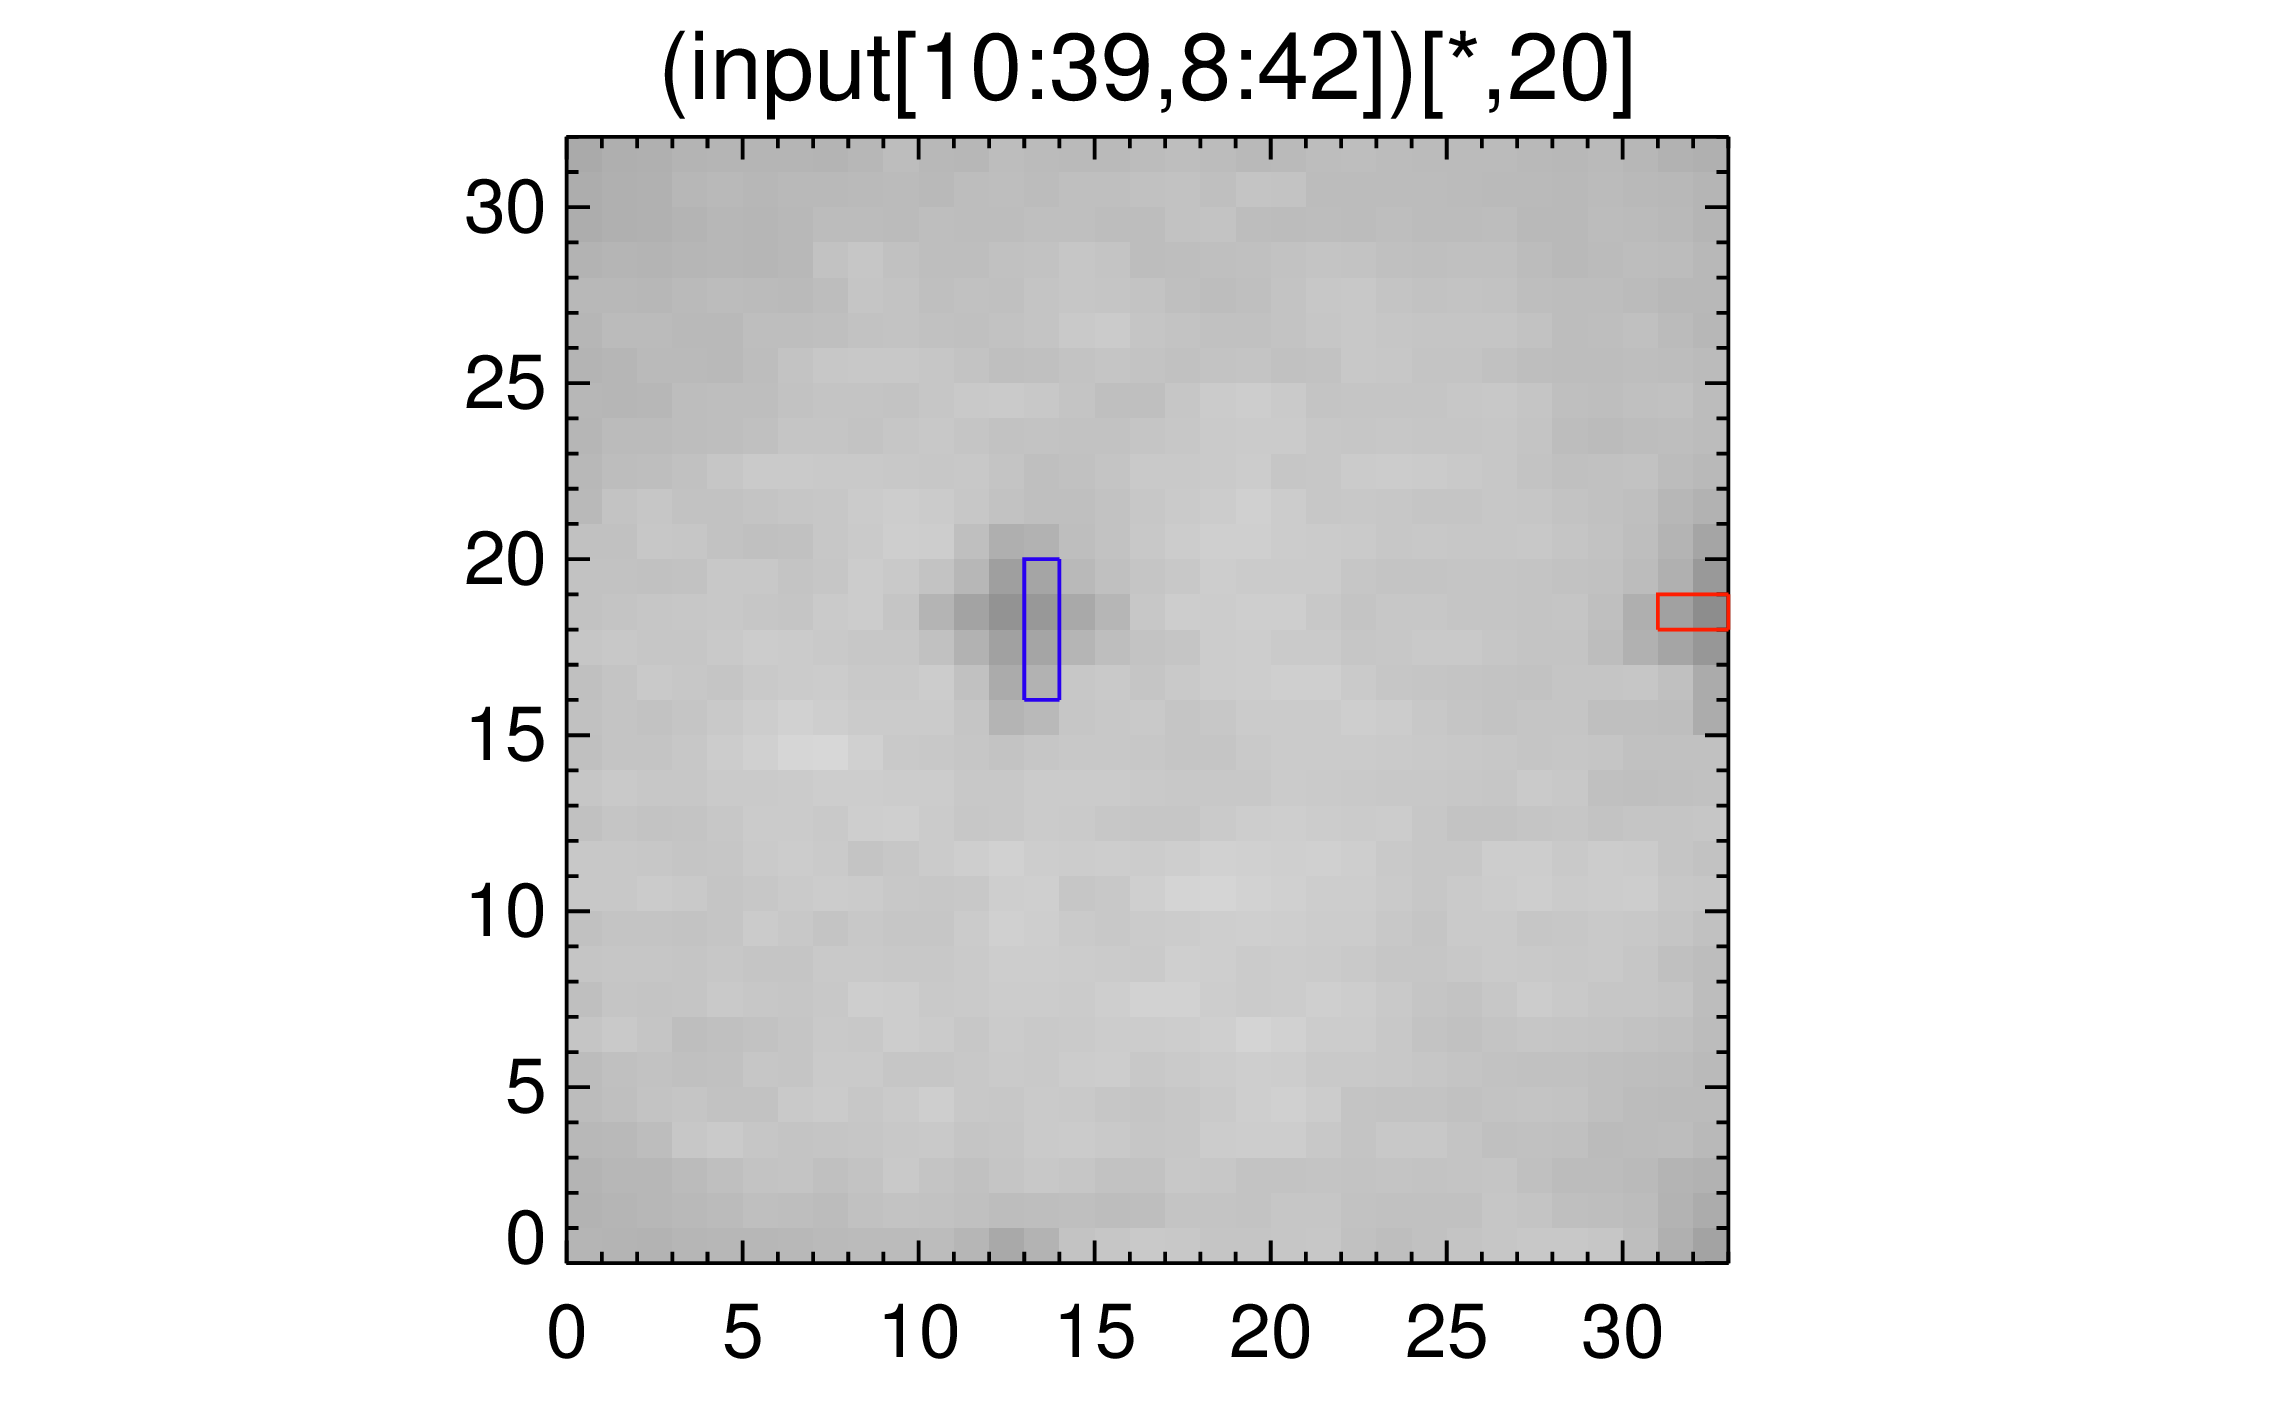
\includegraphics[width=.5\textwidth]{../plots_tables_images/moarfidcheck_withbothtruncate1.png}%
       }%
       {%
       \caption{1 Fiducial pixel in image}%
       }%
        \ffigbox[\Xhsize]%
       {%
       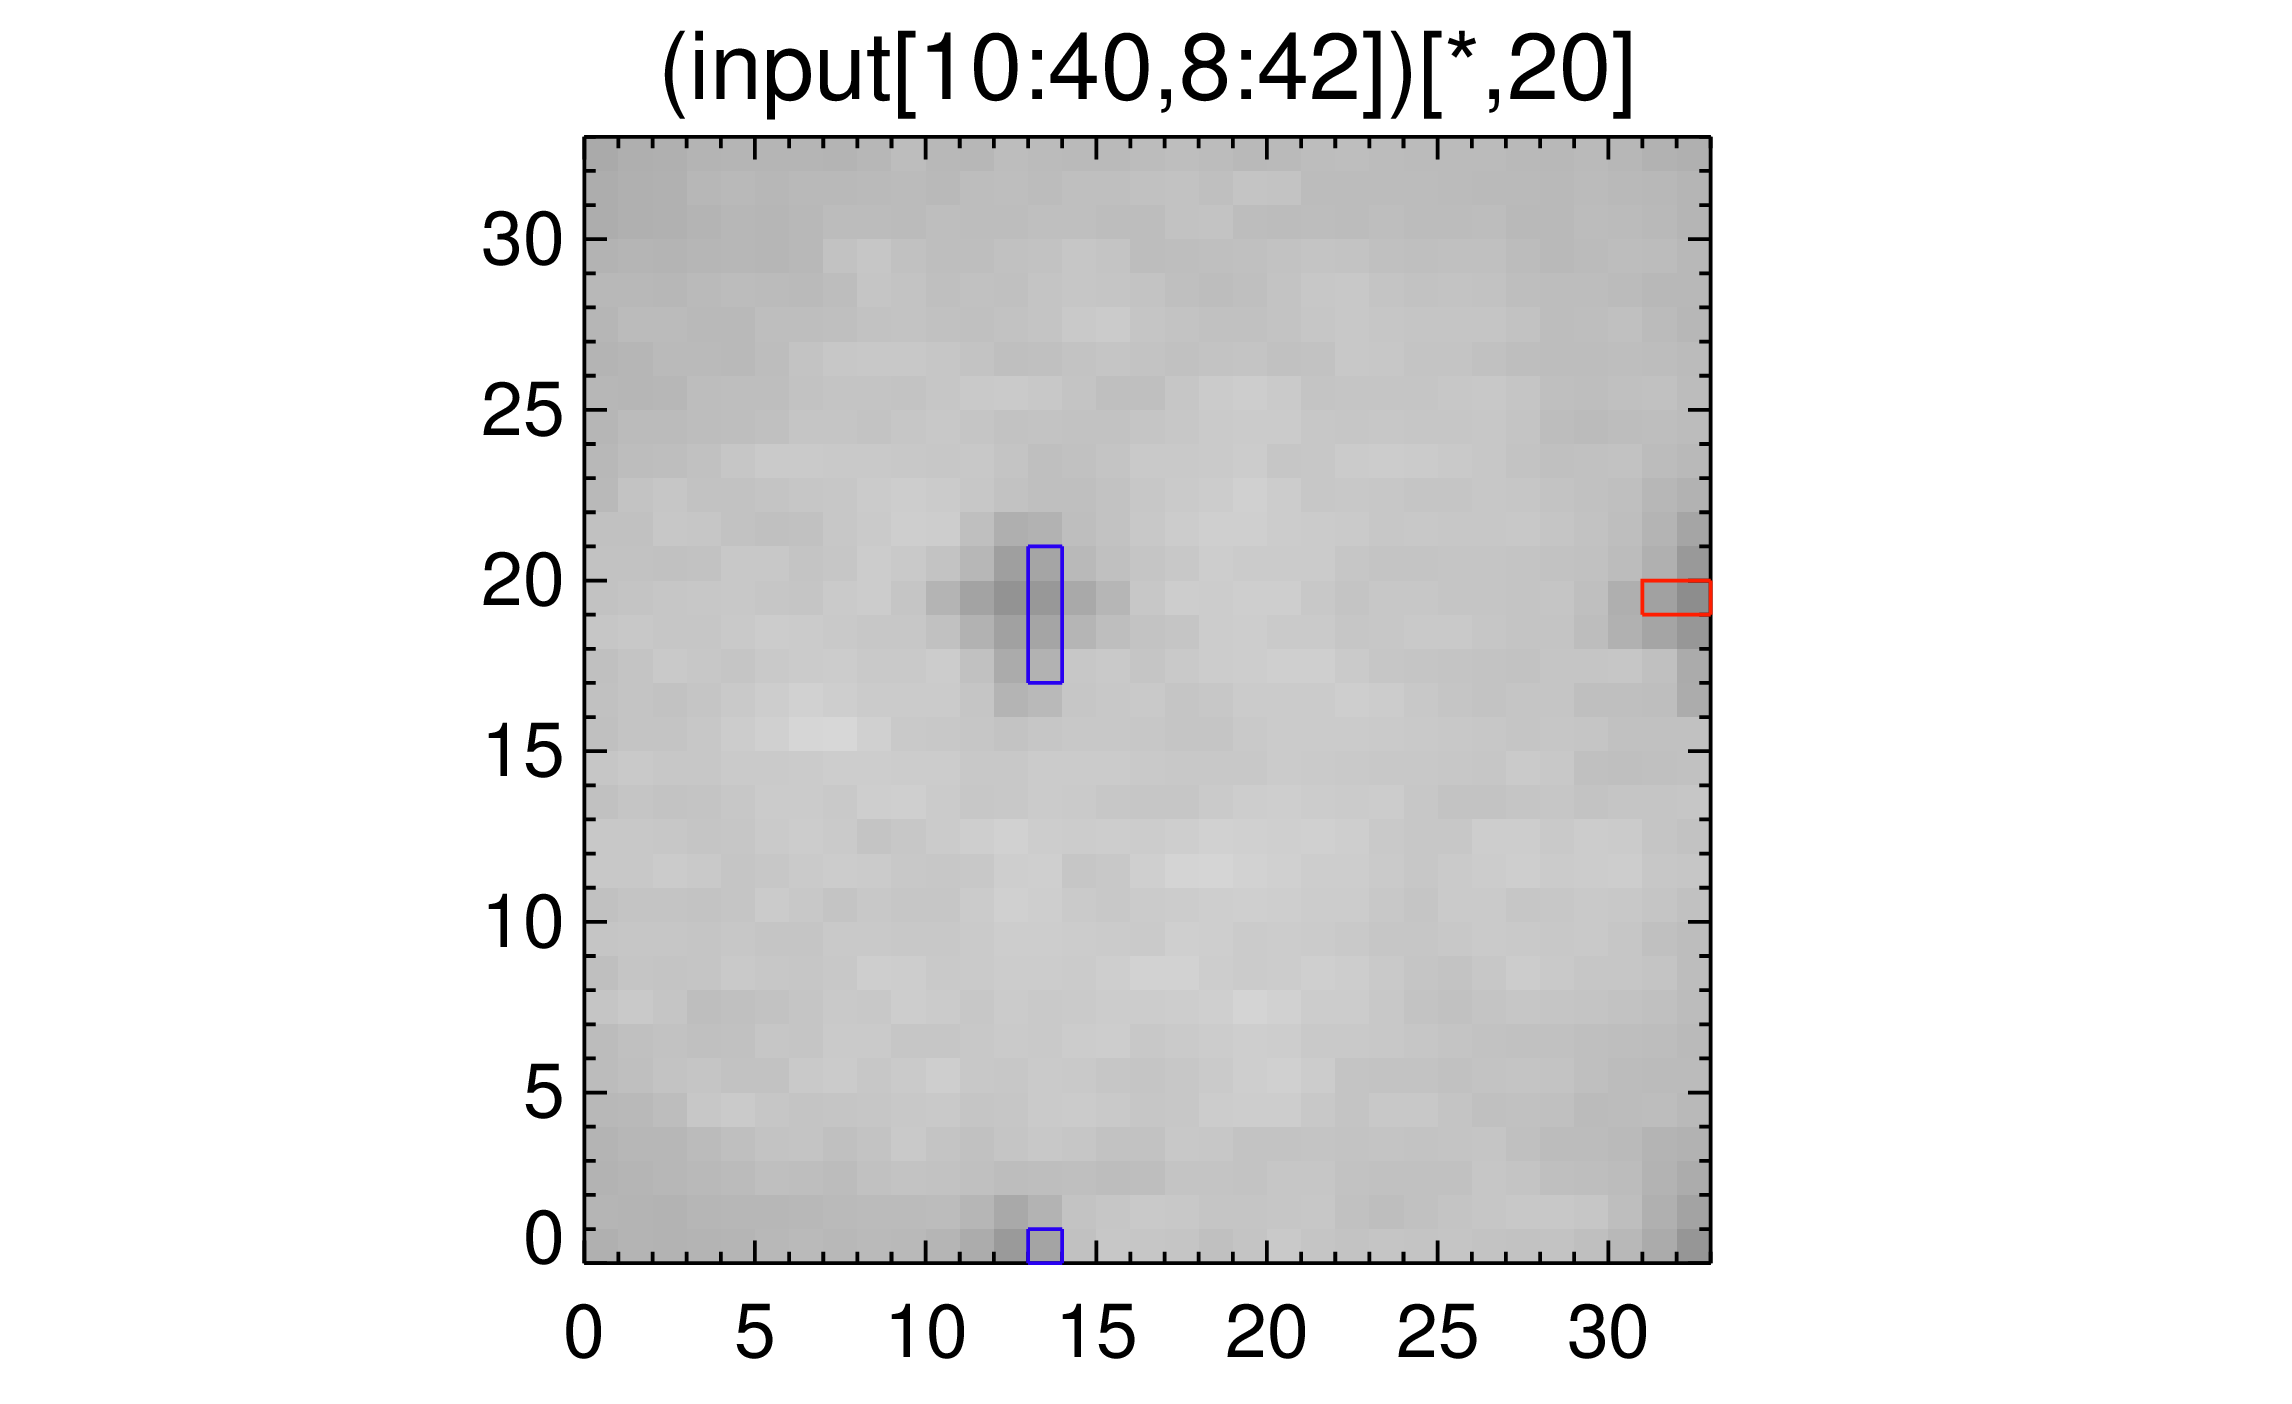
\includegraphics[width=.5\textwidth]{../plots_tables_images/moarfidcheck_withbothtruncate2.png}%
       }%
       {%
       \caption{2 pixels}%
       }%
    \end{subfloatrow}}

    \ffigbox[][\FBheight]{%
    \begin{subfloatrow}[2]%
        \ffigbox[\FBwidth]%
       {%
       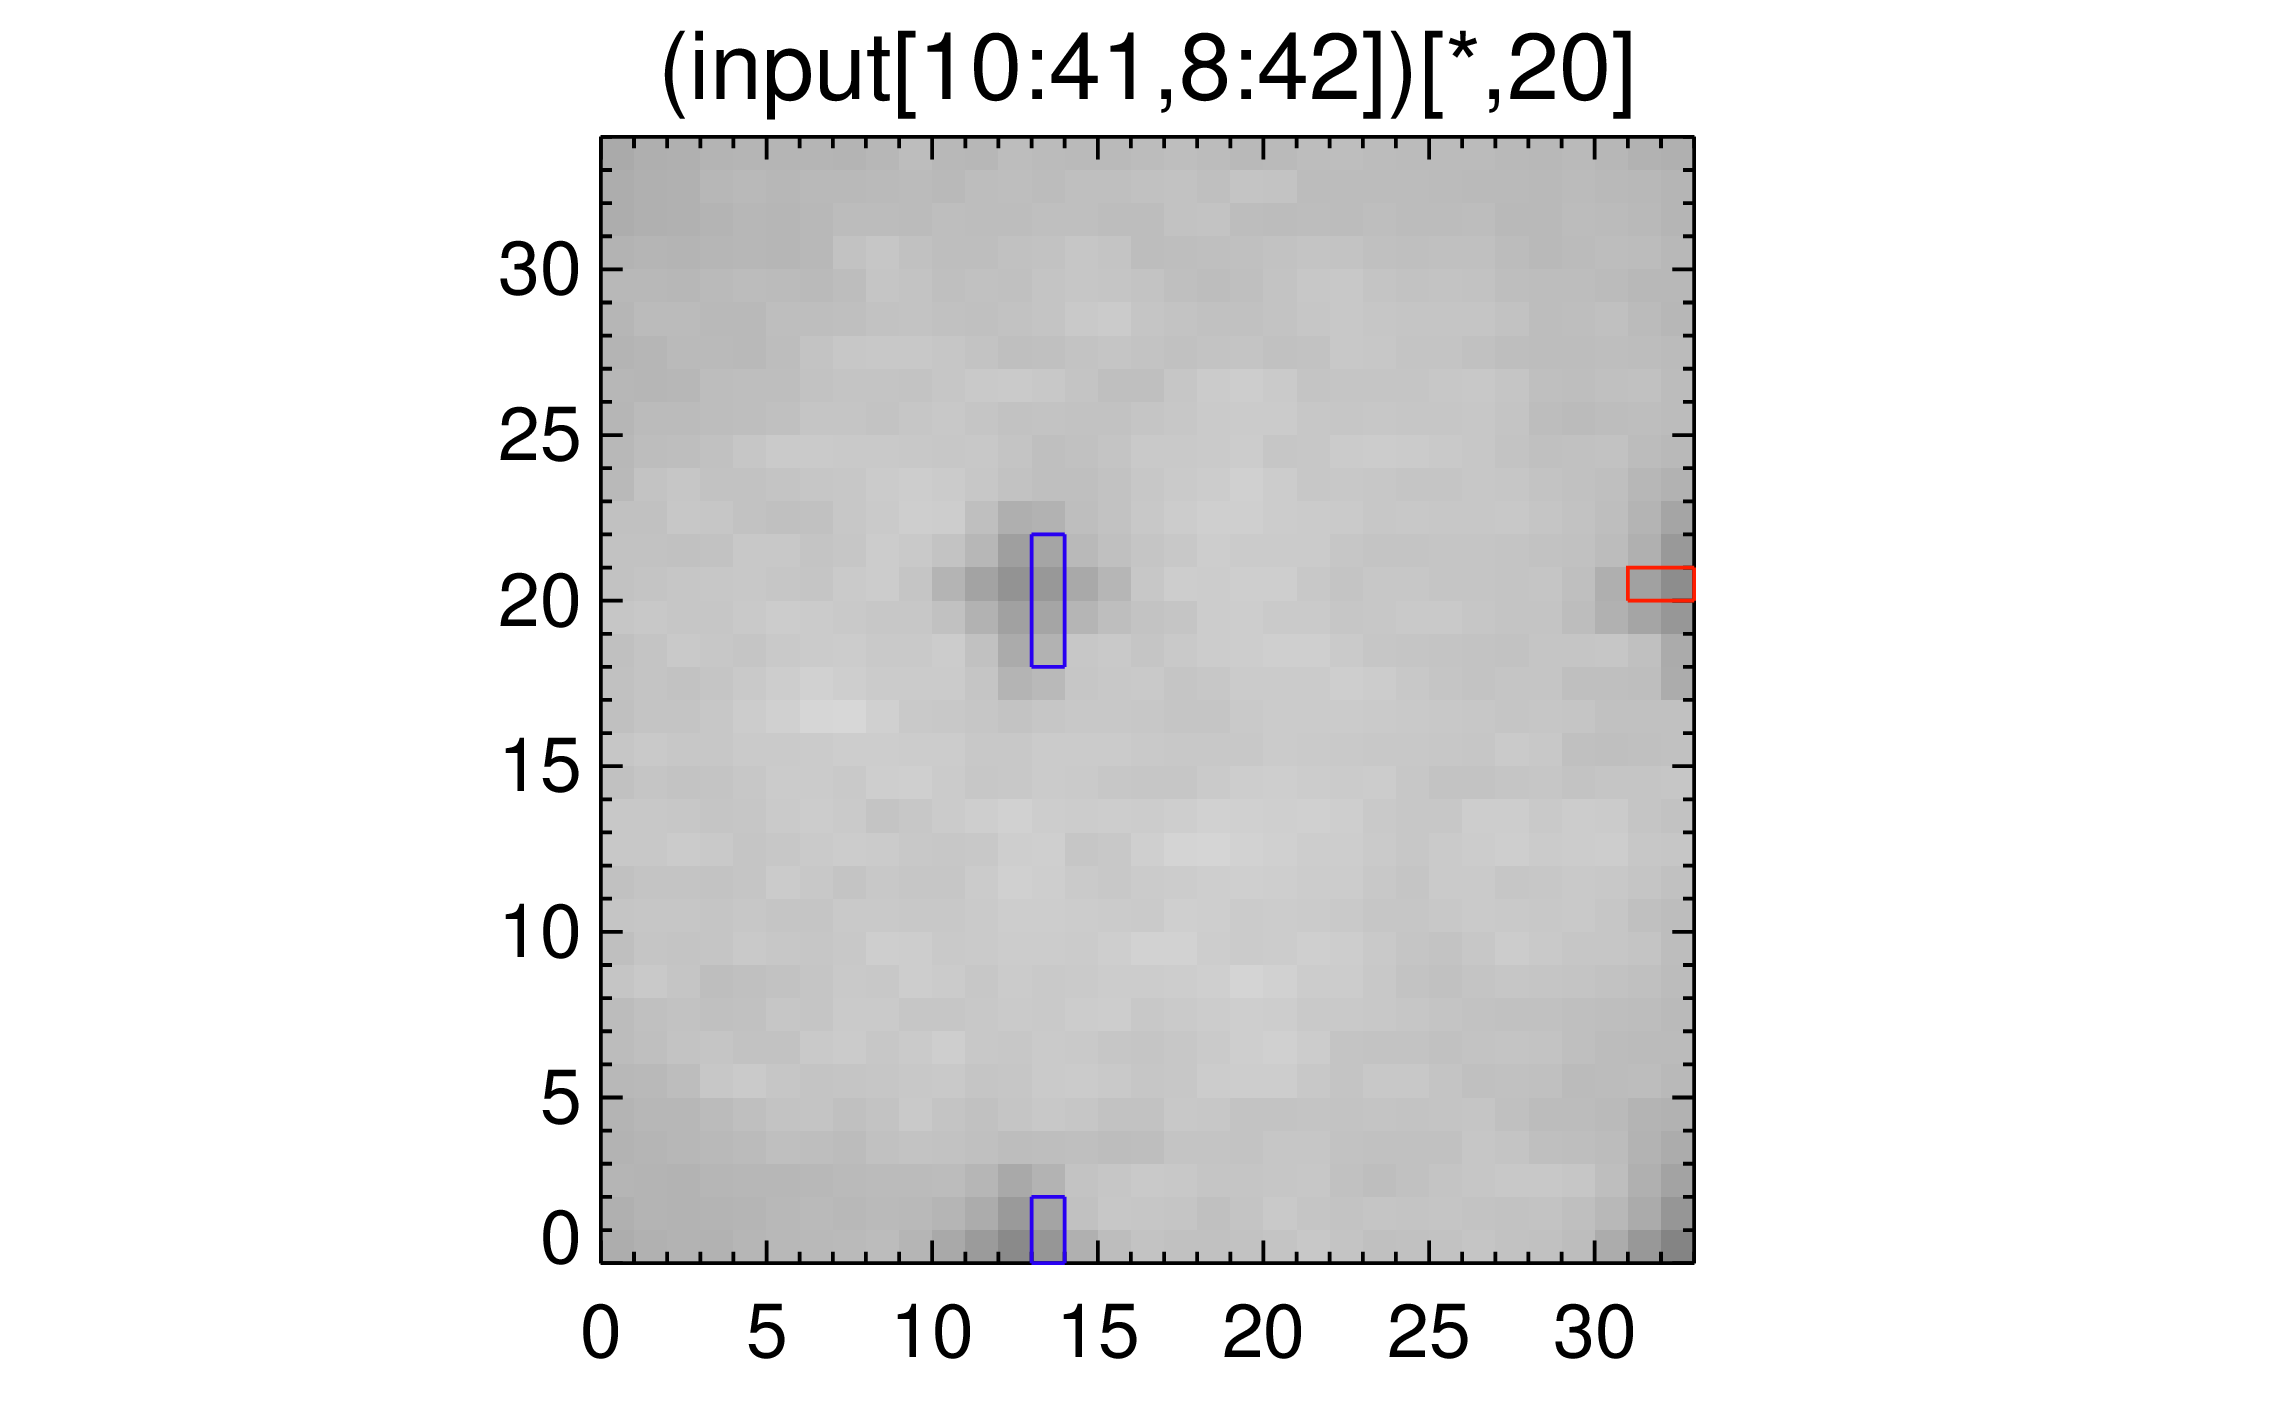
\includegraphics[width=.5\textwidth]{../plots_tables_images/moarfidcheck_withbothtruncate3.png}%
       }%
       {%
       \caption{3 pixels}%
       }%
        \ffigbox[\Xhsize]%
       {%
       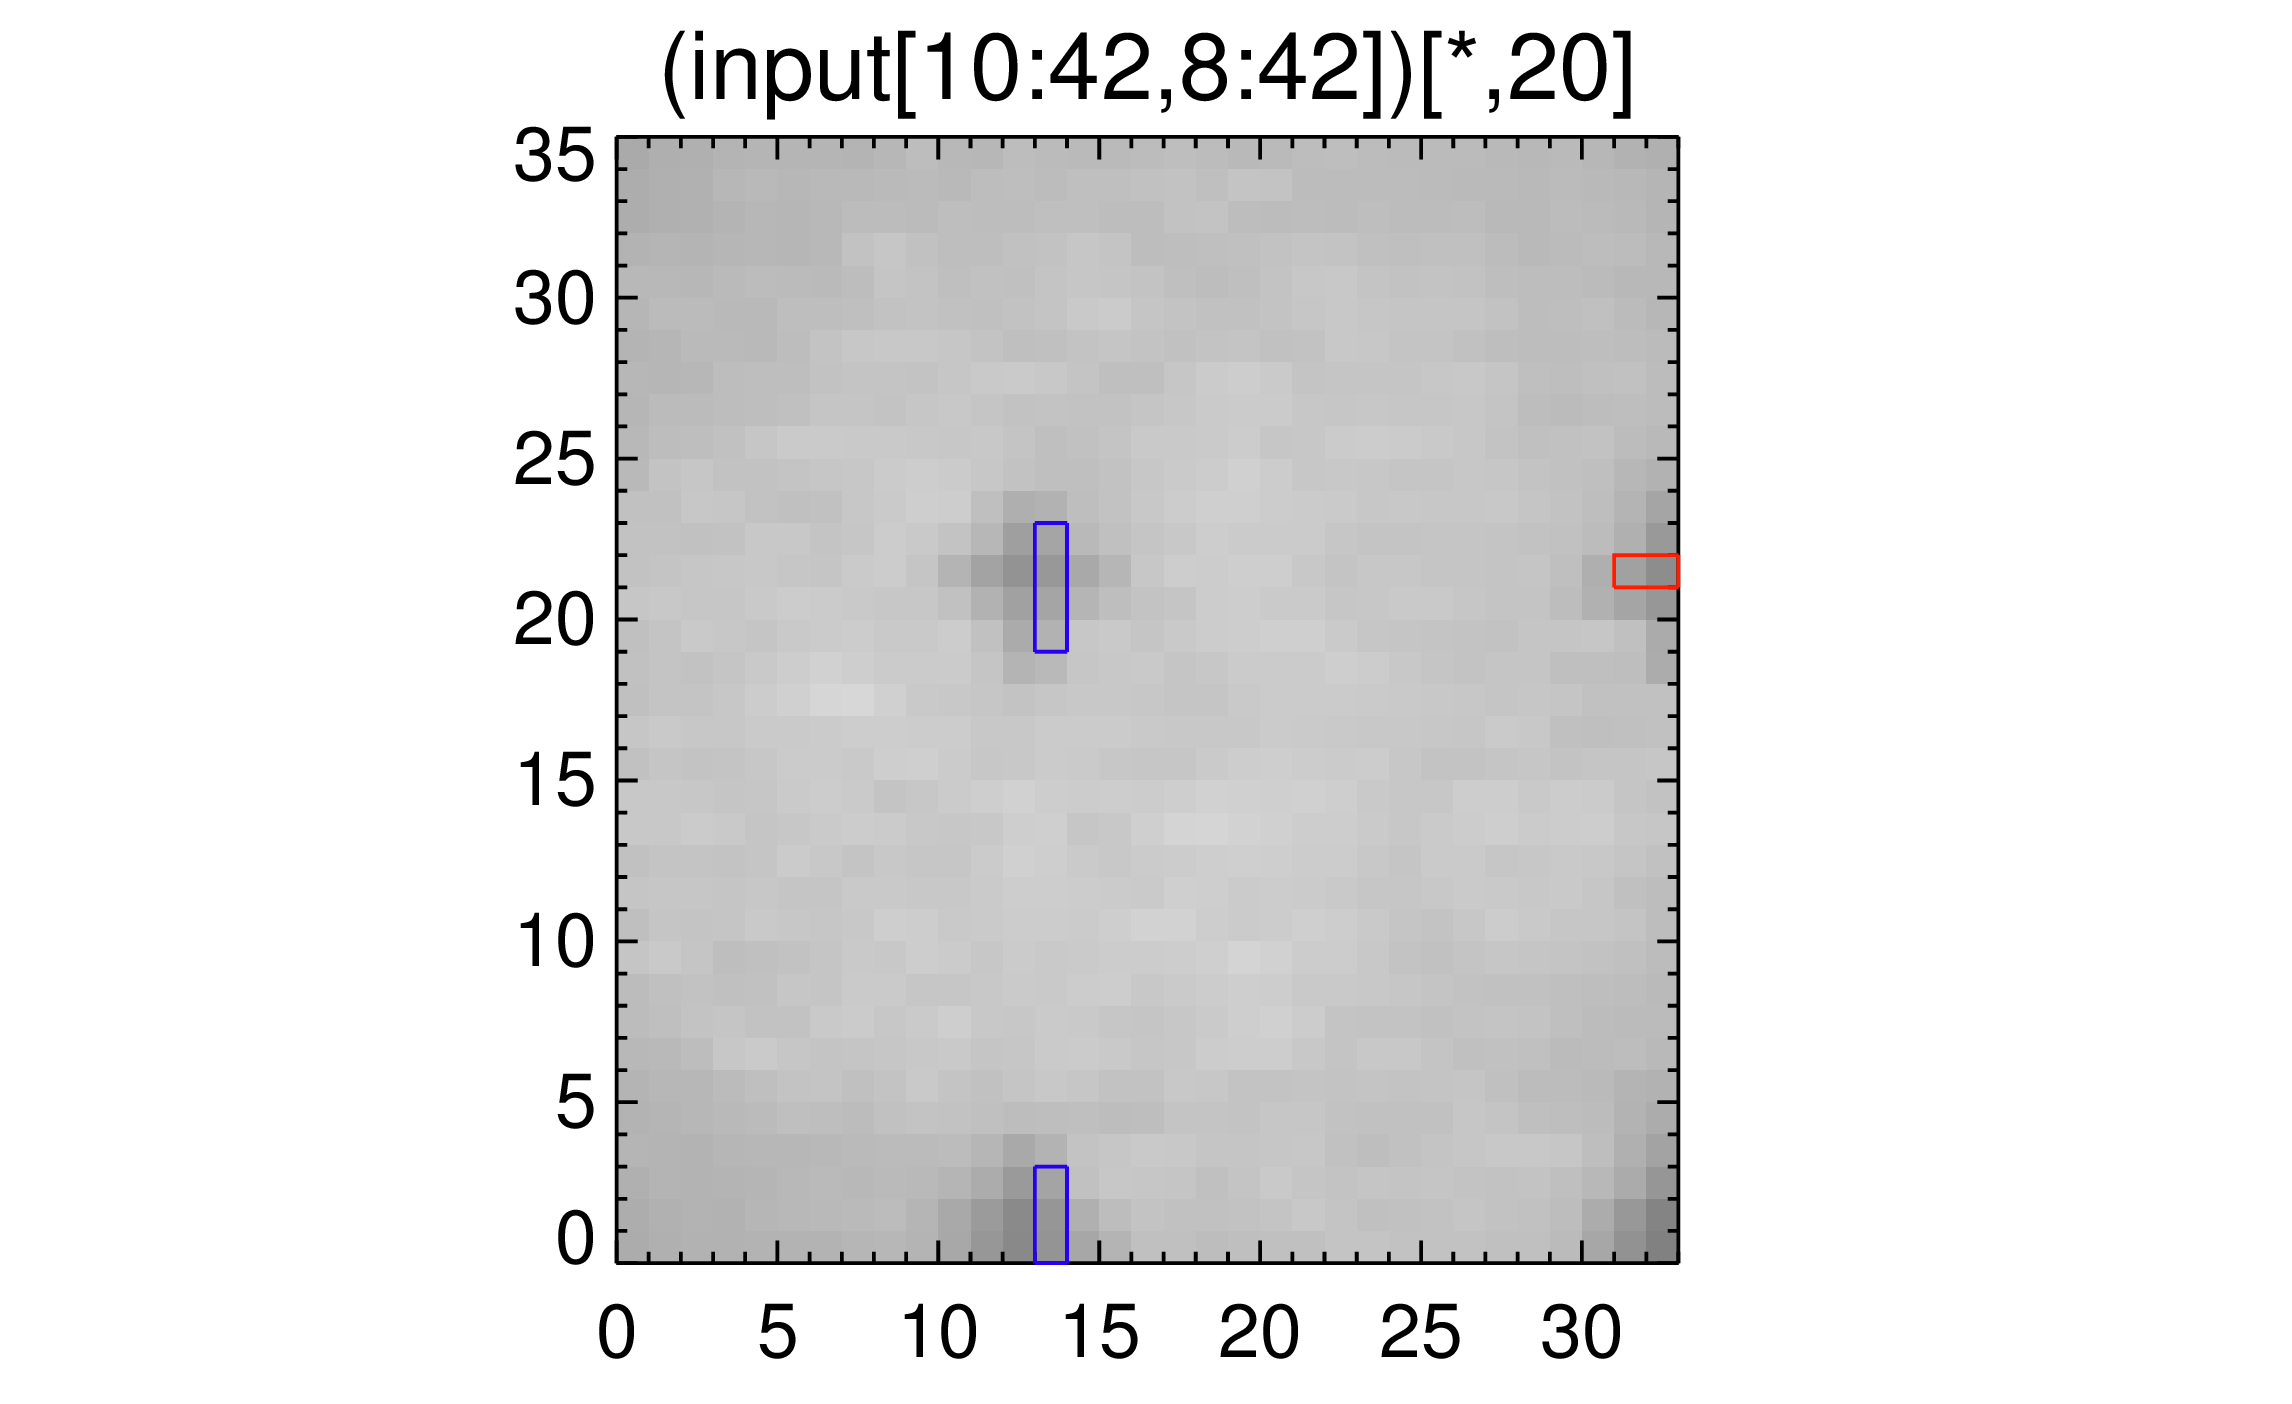
\includegraphics[width=.5\textwidth]{../plots_tables_images/moarfidcheck_withbothtruncate4.png}%
       }%
       {%
       \caption{4 pixels}%
       }%
    \end{subfloatrow}}

    \ffigbox[][\FBheight]{%
    \begin{subfloatrow}[2]%
        \ffigbox[\FBwidth]%
       {%
       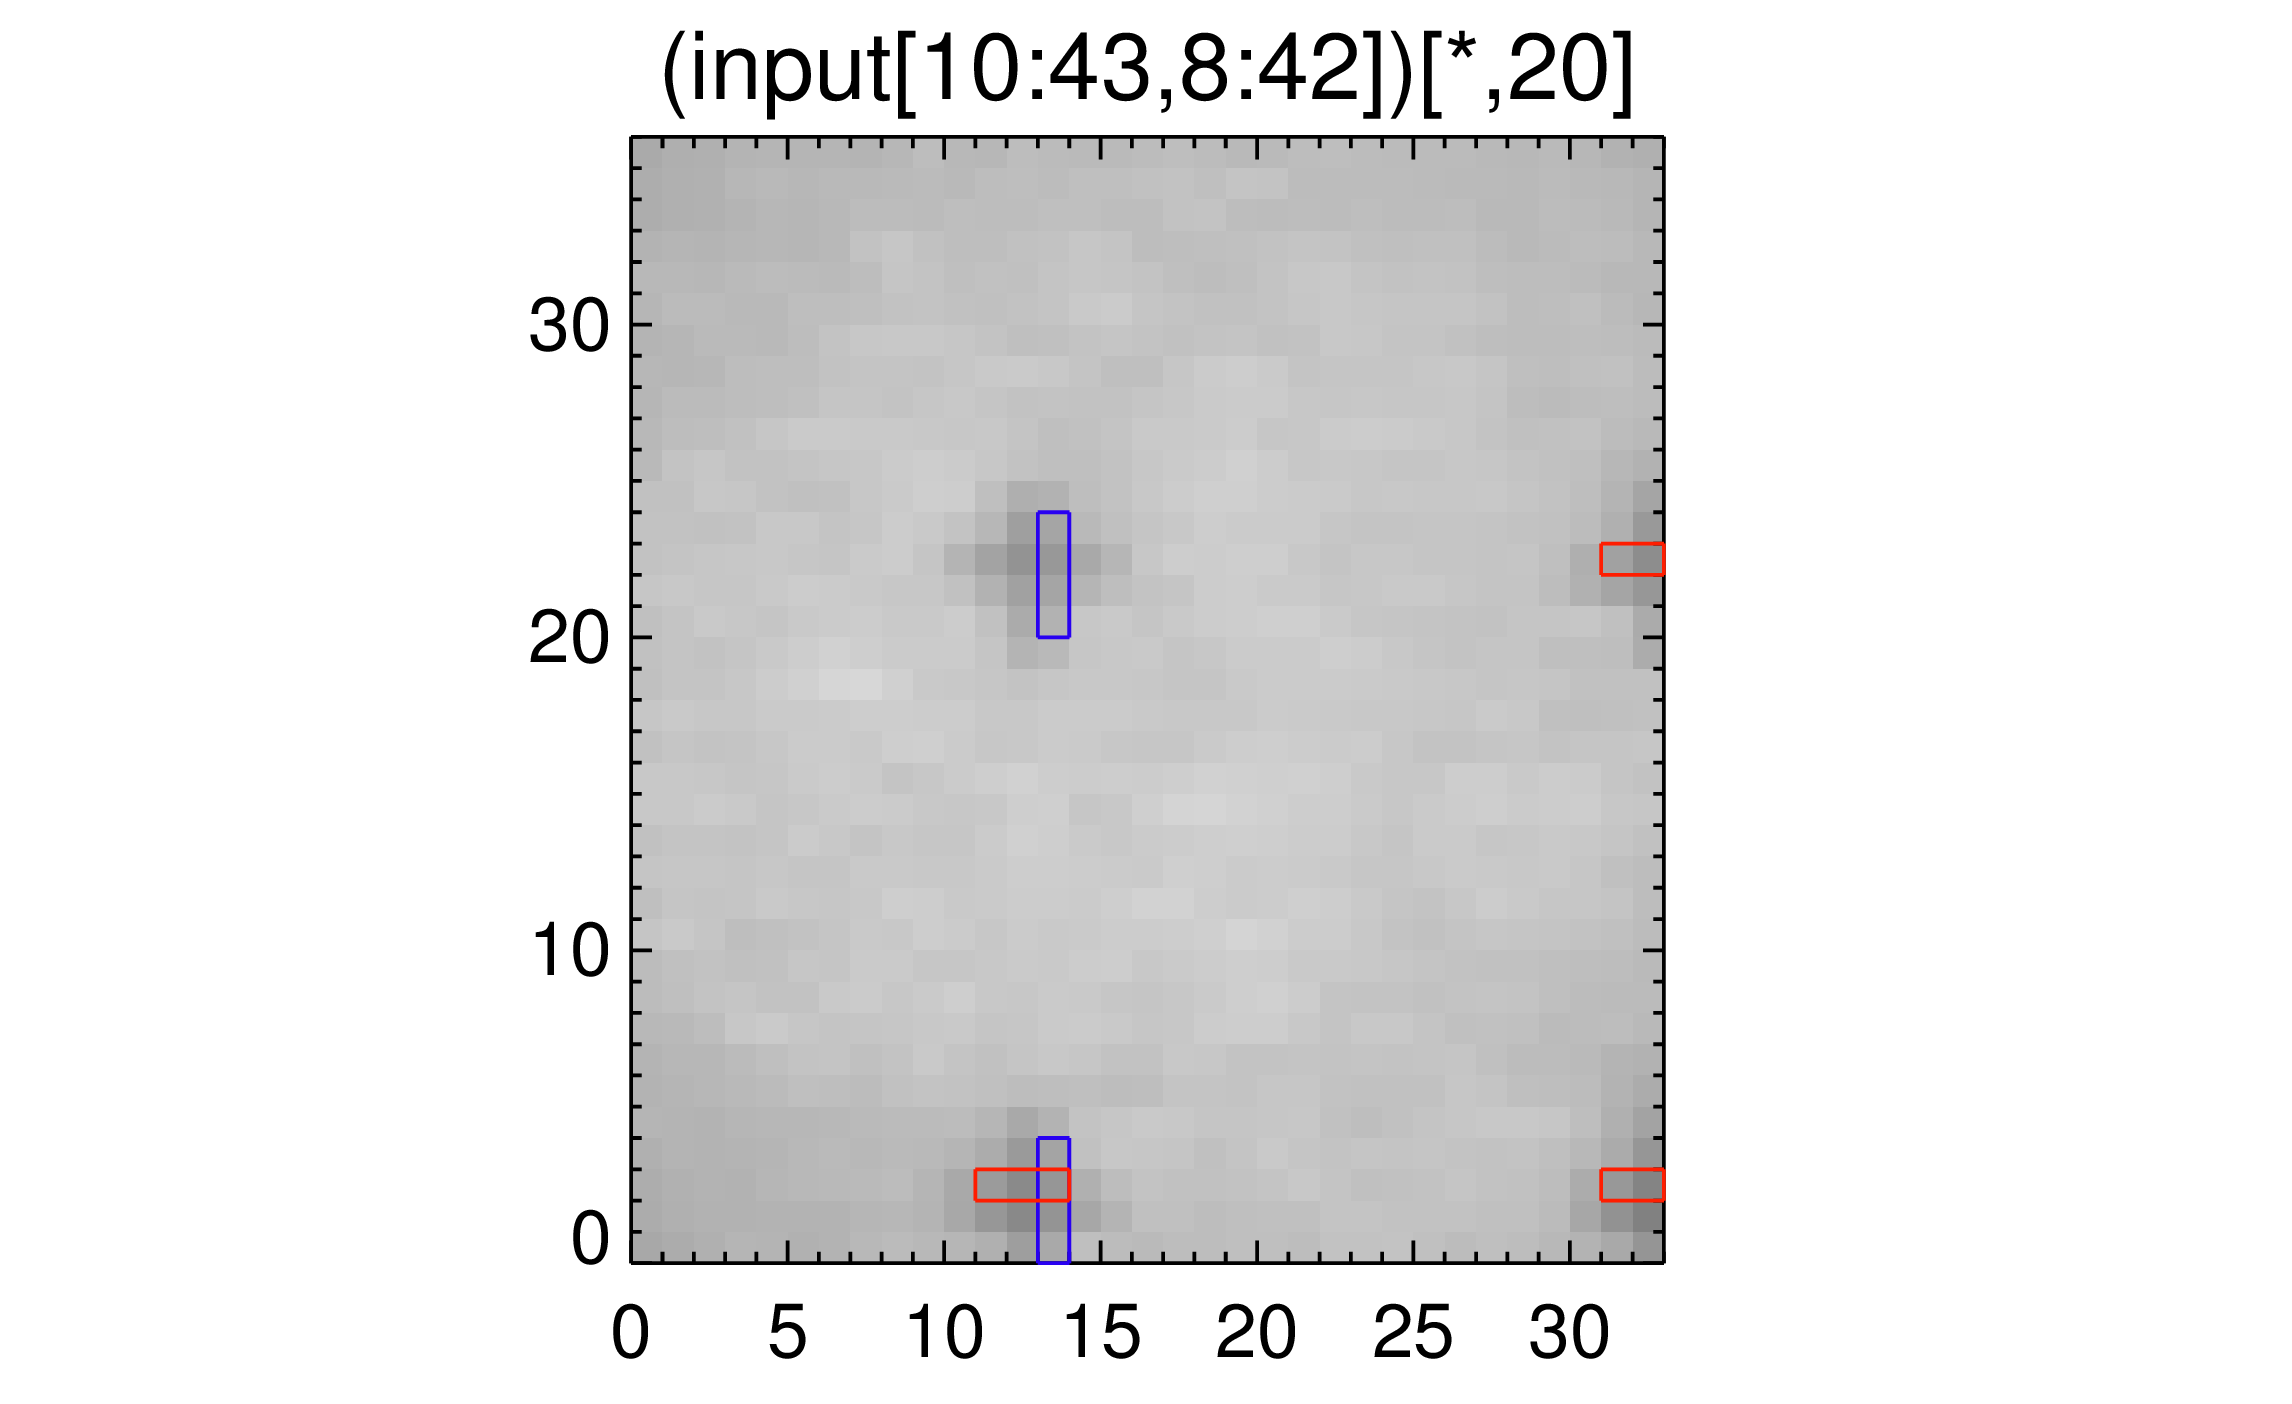
\includegraphics[width=.5\textwidth]{../plots_tables_images/moarfidcheck_withbothtruncate5.png}%
       }%
       {%
       \caption{5 pixels}%
       }%
        \ffigbox[\Xhsize]%
       {%
       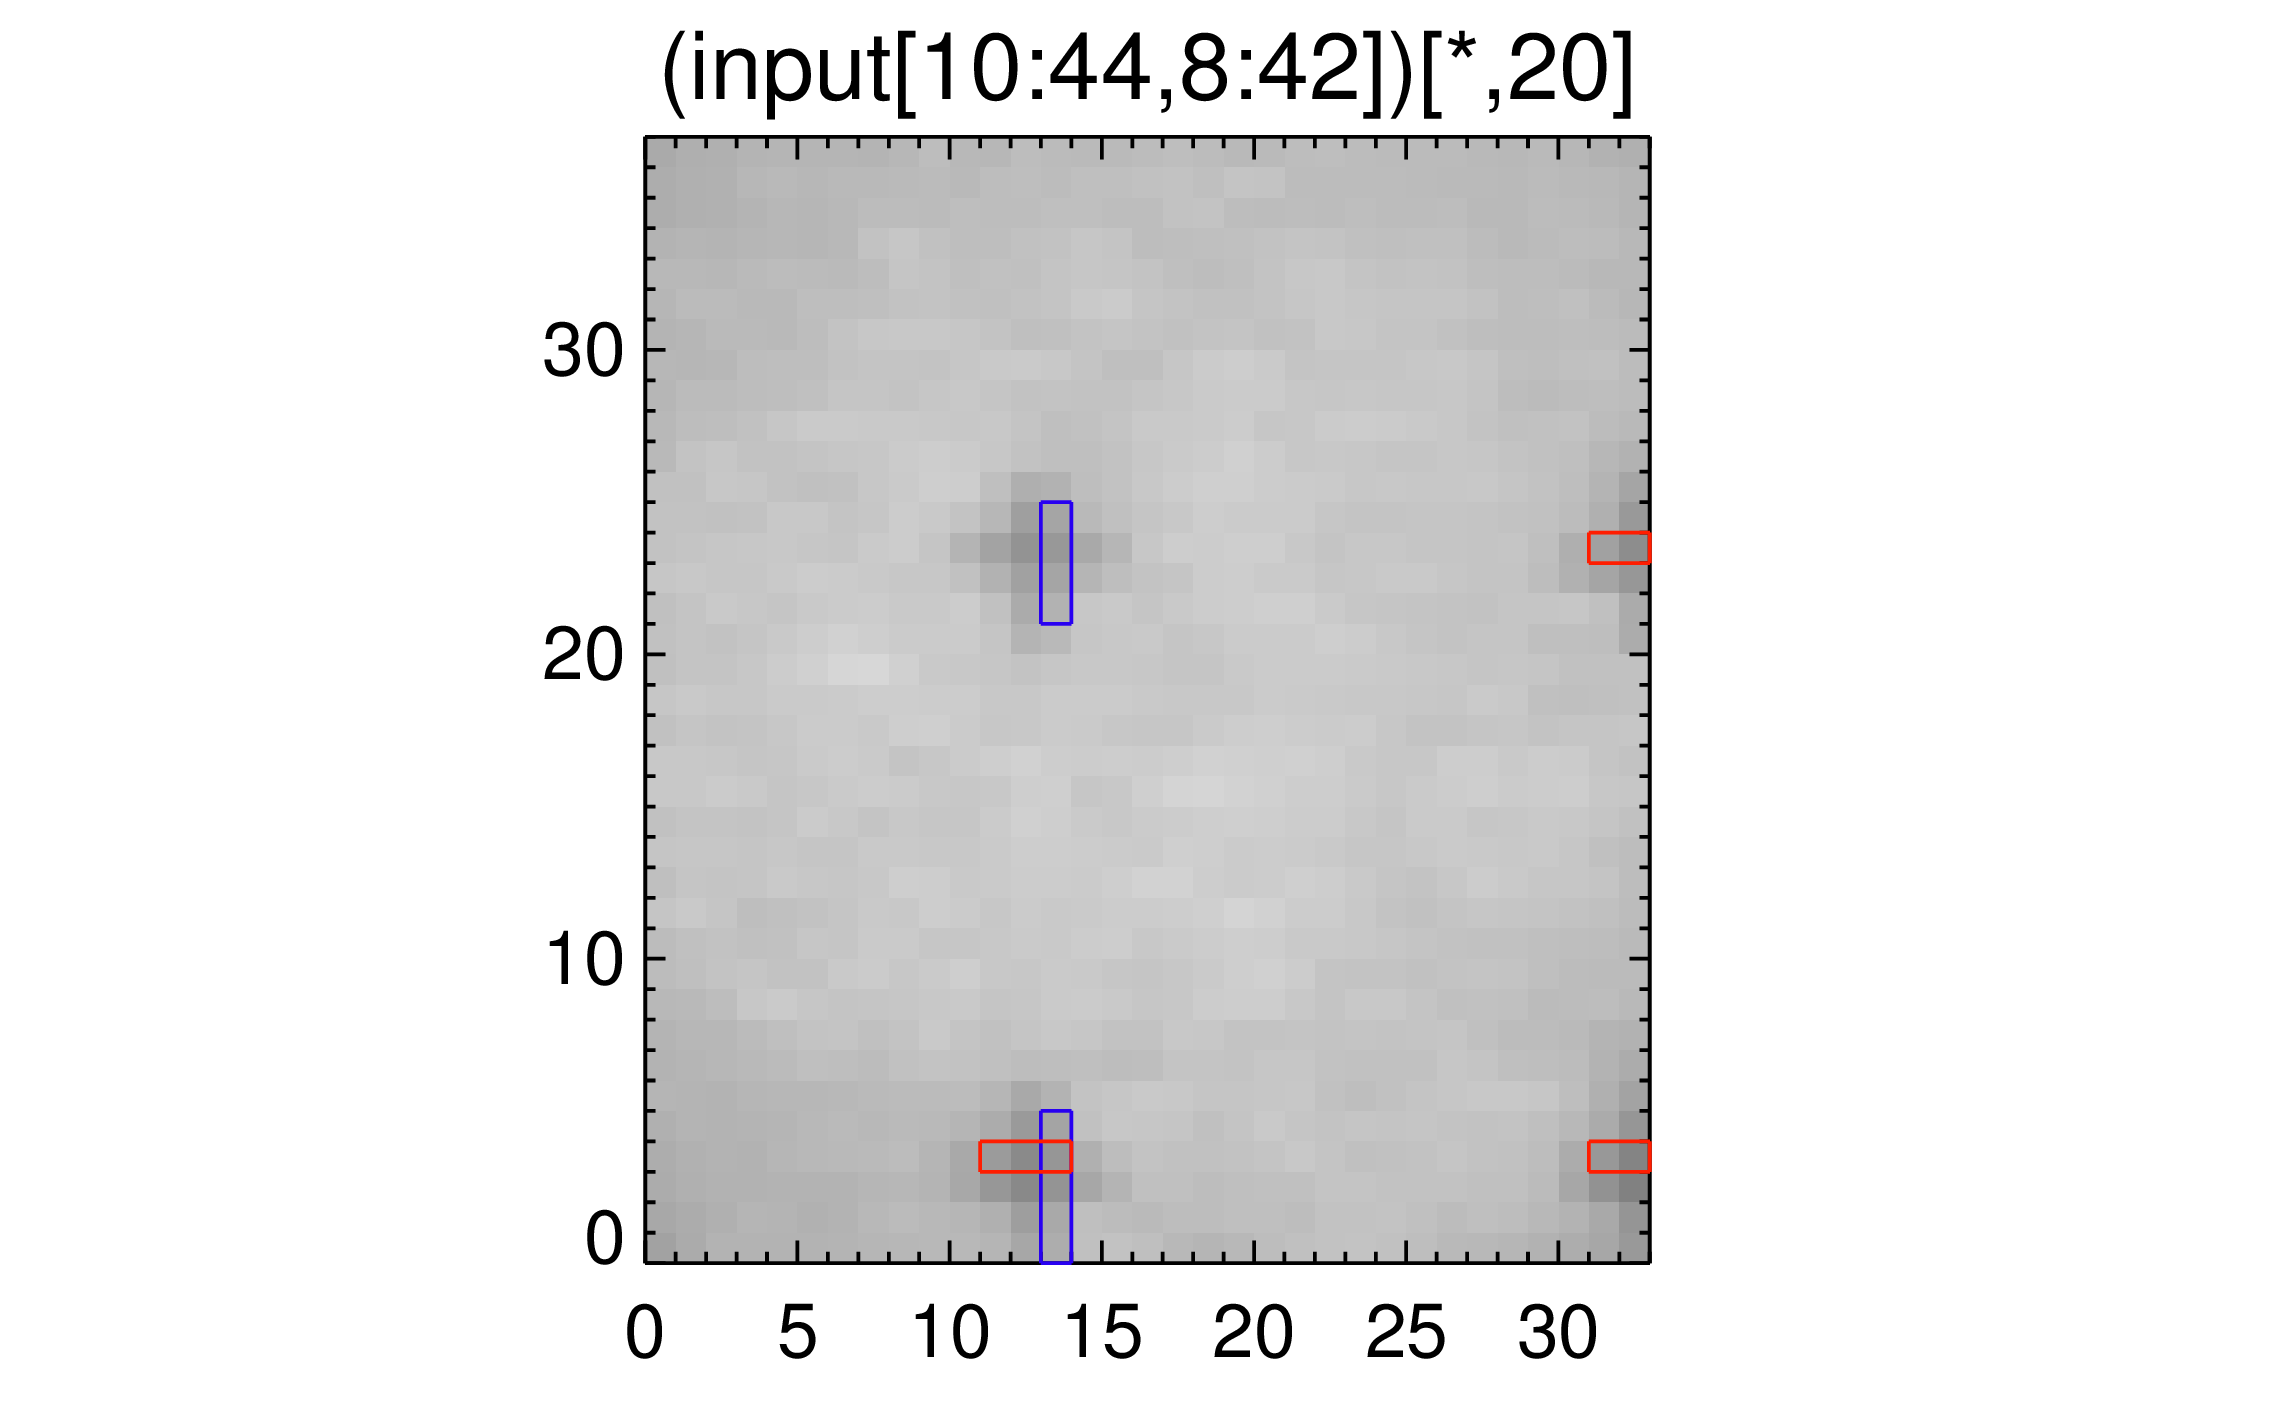
\includegraphics[width=.5\textwidth]{../plots_tables_images/moarfidcheck_withbothtruncate6.png}%
       }%
       {%
       \caption{Completely in image}%
       }%
    \end{subfloatrow}}{\caption{This time, we're cropping the bottom less and less}\label{firstplot}}
\end{figure}

% \begin{figure}[!h]
%     \centering 
%     \begin{subfigure}[b]{.45\linewidth}
%         \centering
%         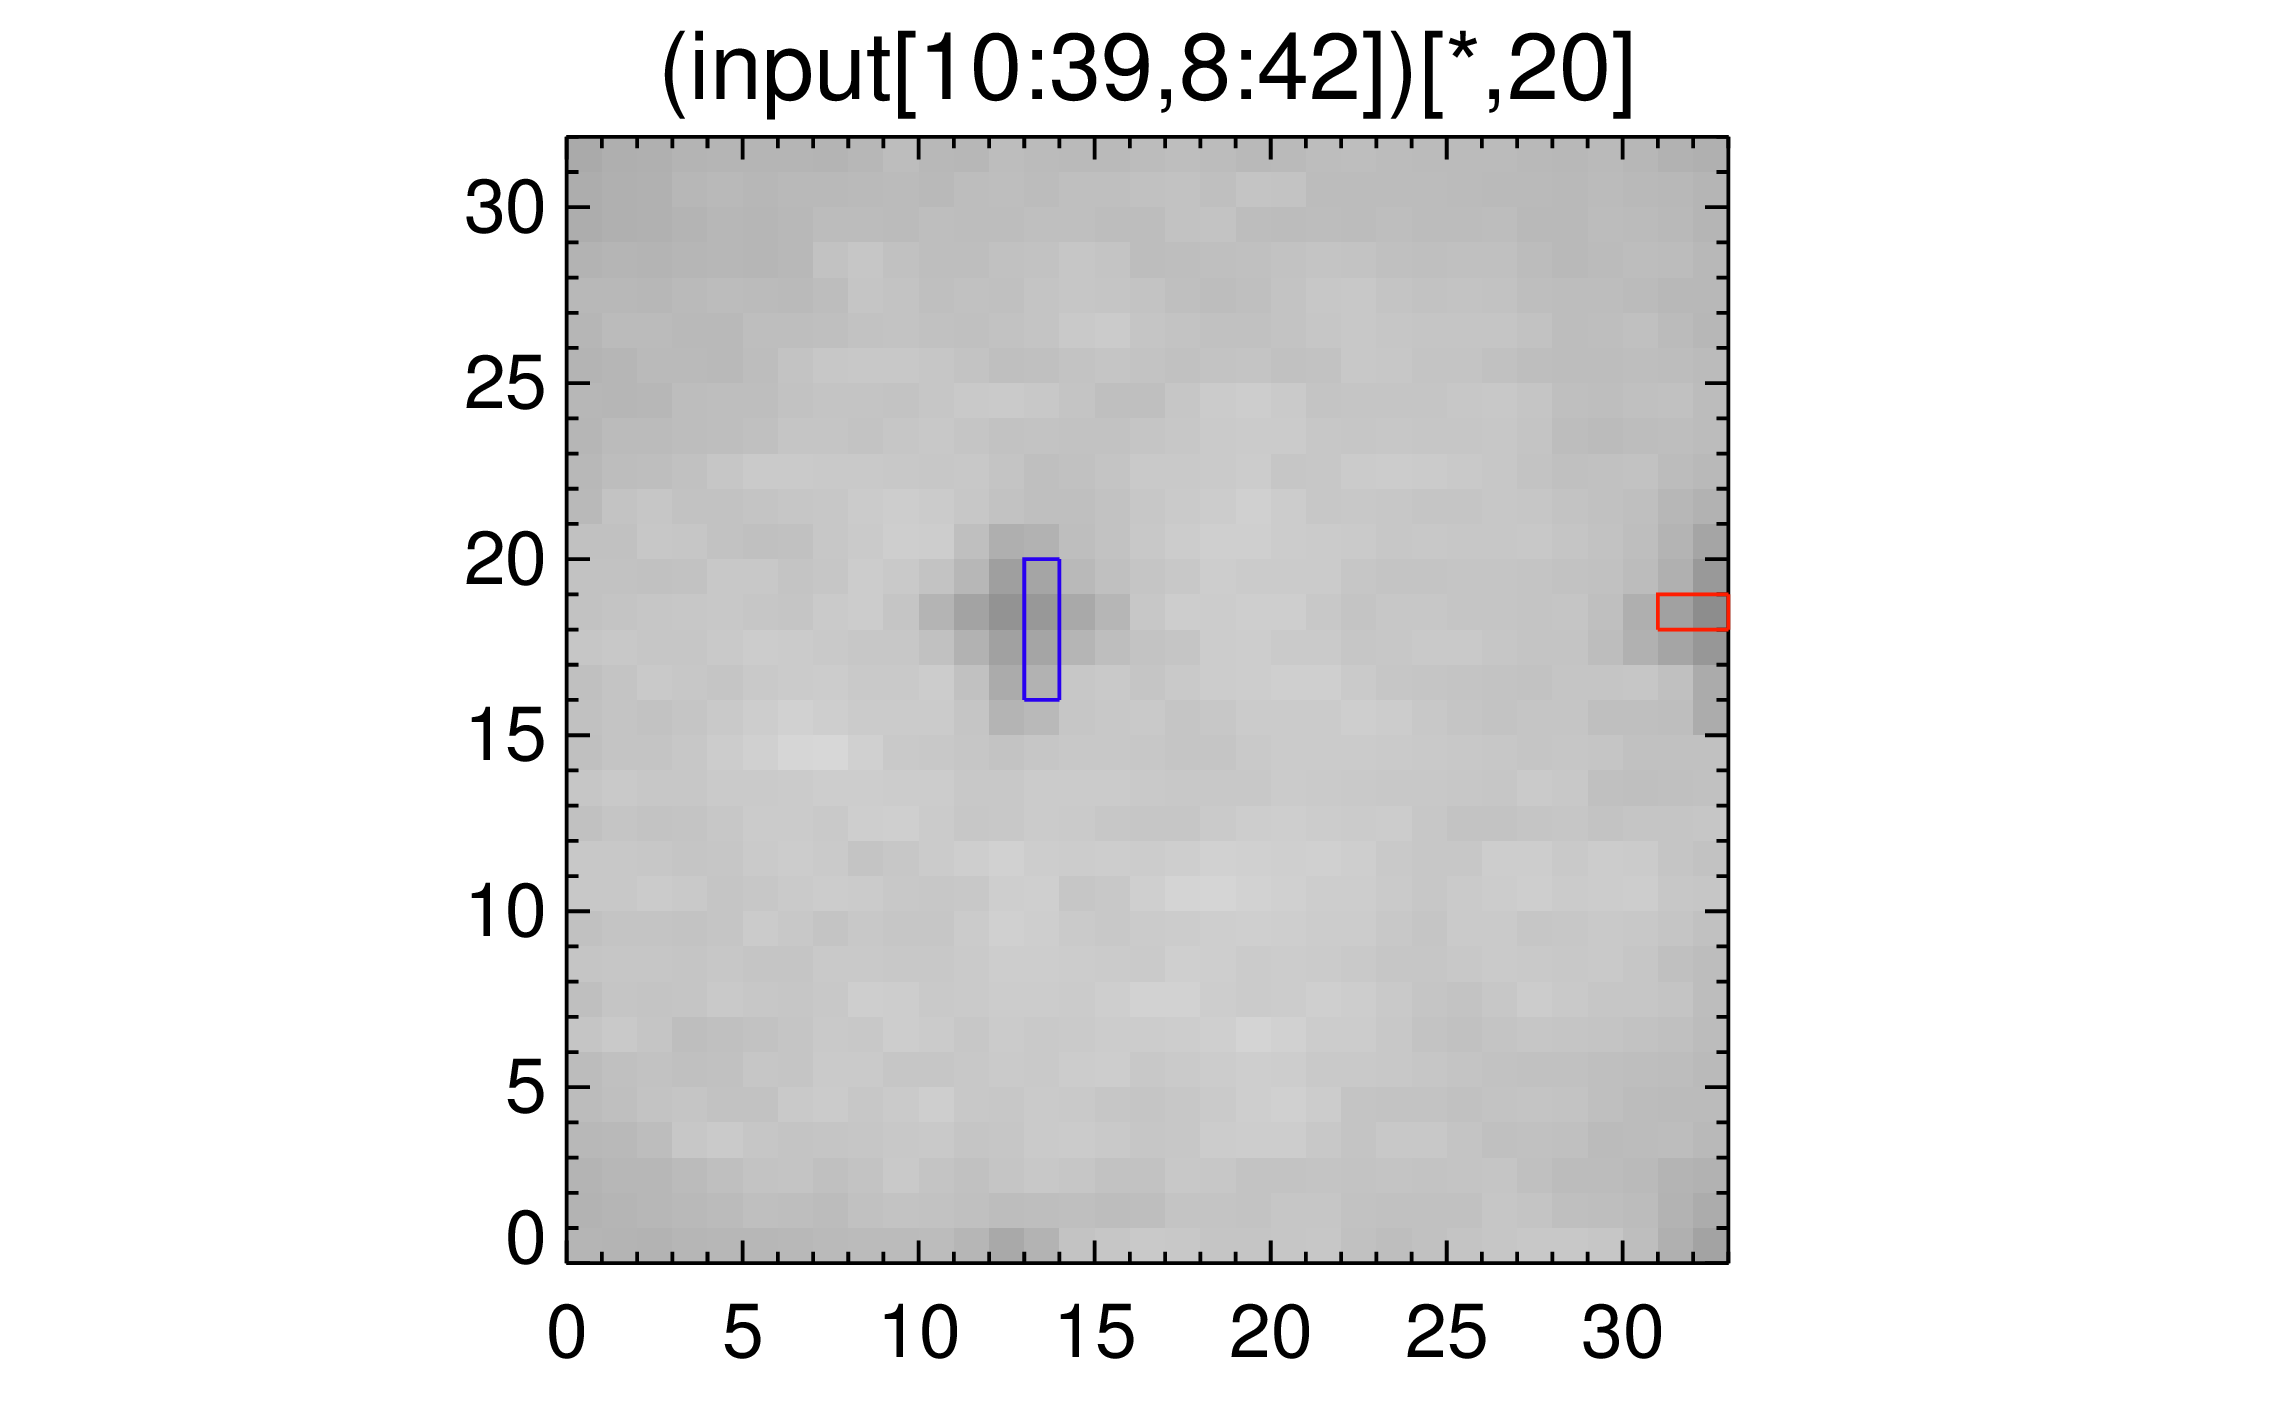
\includegraphics[width=1.3\textwidth]{../plots_tables_images/moarfidcheck_withbothtruncate1.png}
%         \caption{1 Fiducial pixel in image}
%     \end{subfigure}
%     \begin{subfigure}[b]{.45\linewidth}
%         \centering
%         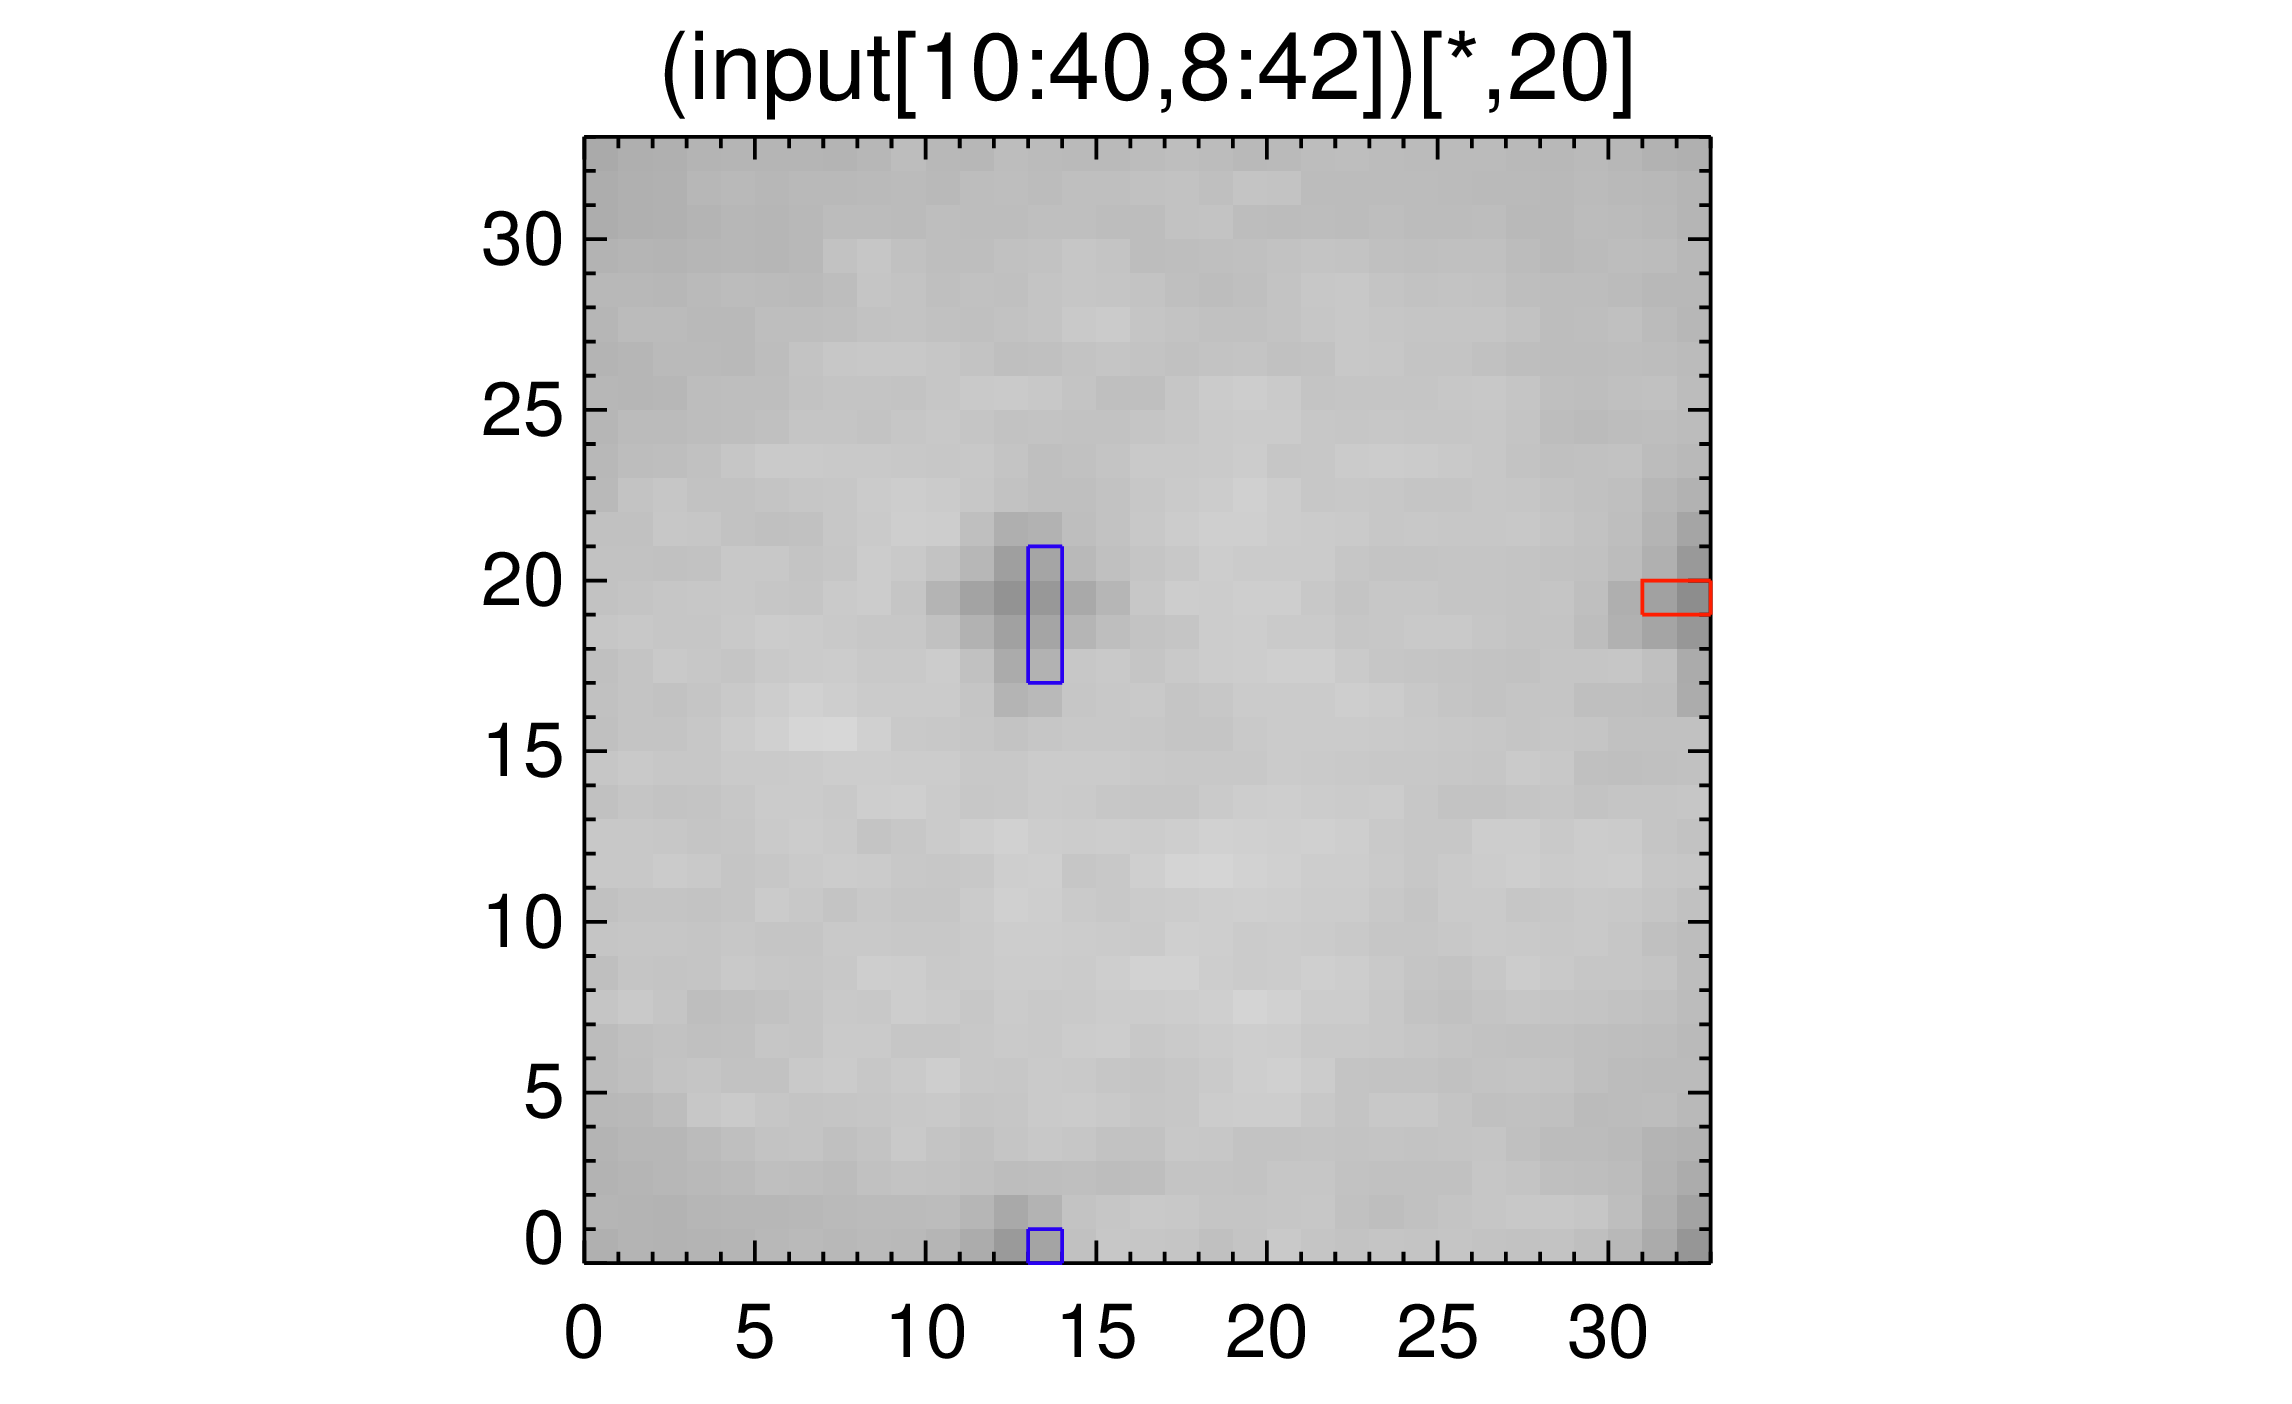
\includegraphics[width=1.3\textwidth]{../plots_tables_images/moarfidcheck_withbothtruncate2.png}
%         \caption{2 pixels}
%     \end{subfigure}
   
%    \begin{subfigure}[b]{.45\linewidth}
%         \centering
%         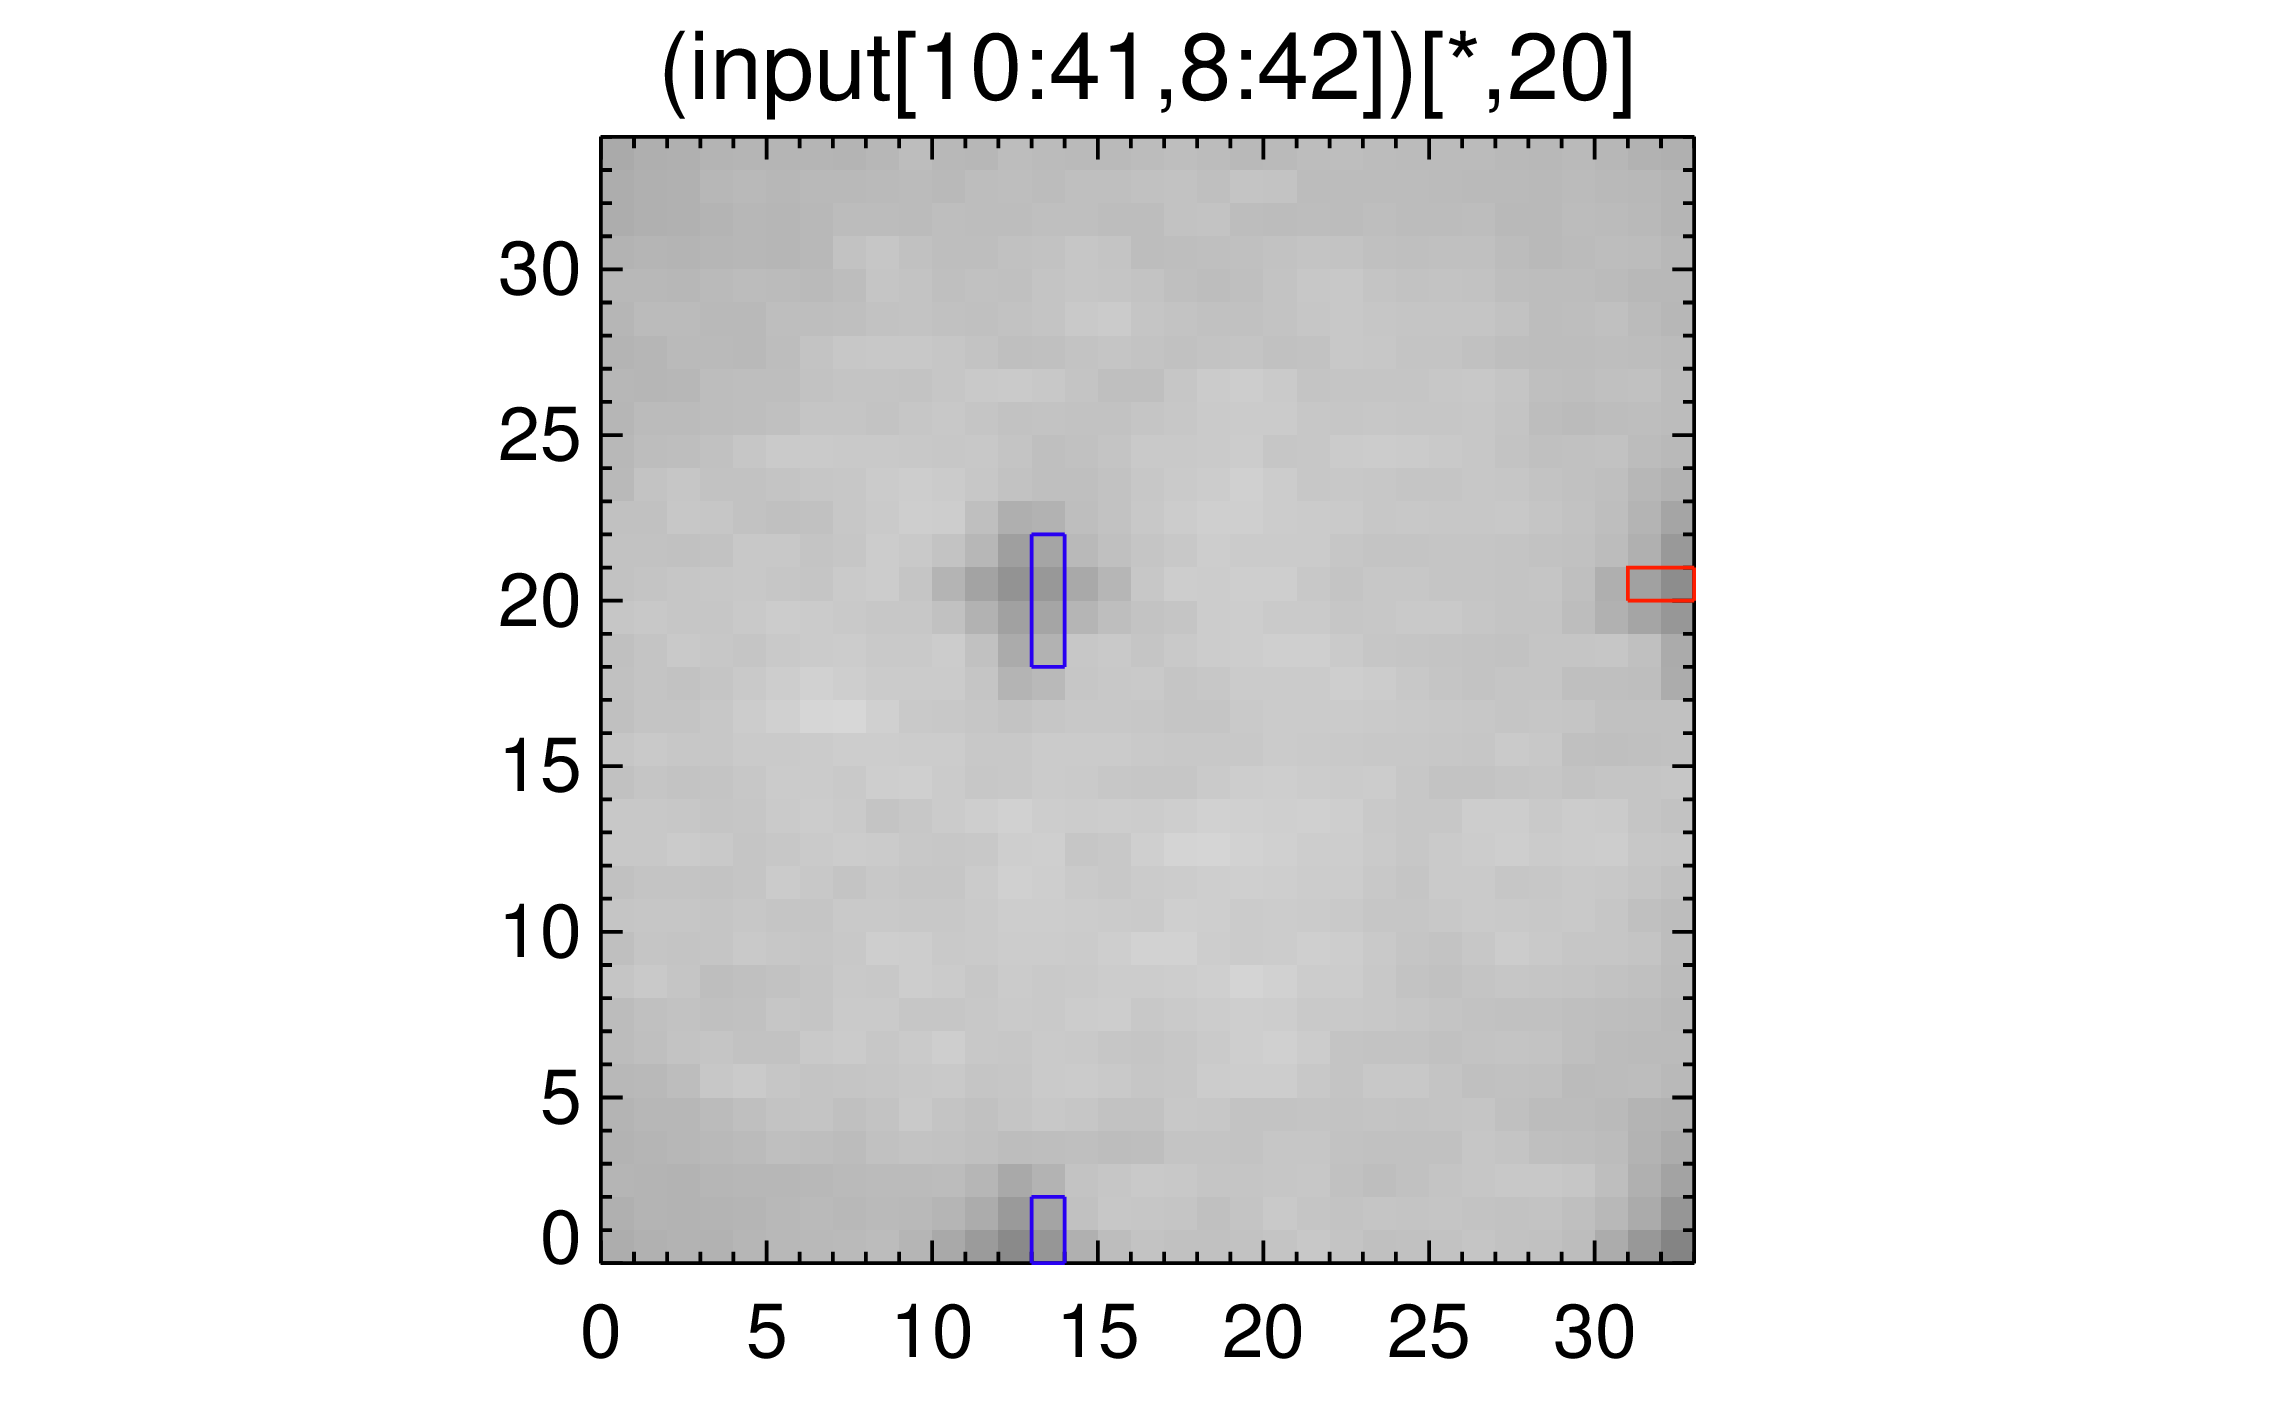
\includegraphics[width=1.3\textwidth]{../plots_tables_images/moarfidcheck_withbothtruncate3.png}
%         \caption{3 pixels}
%     \end{subfigure}
%     \begin{subfigure}[b]{.45\linewidth}
%         \centering
%         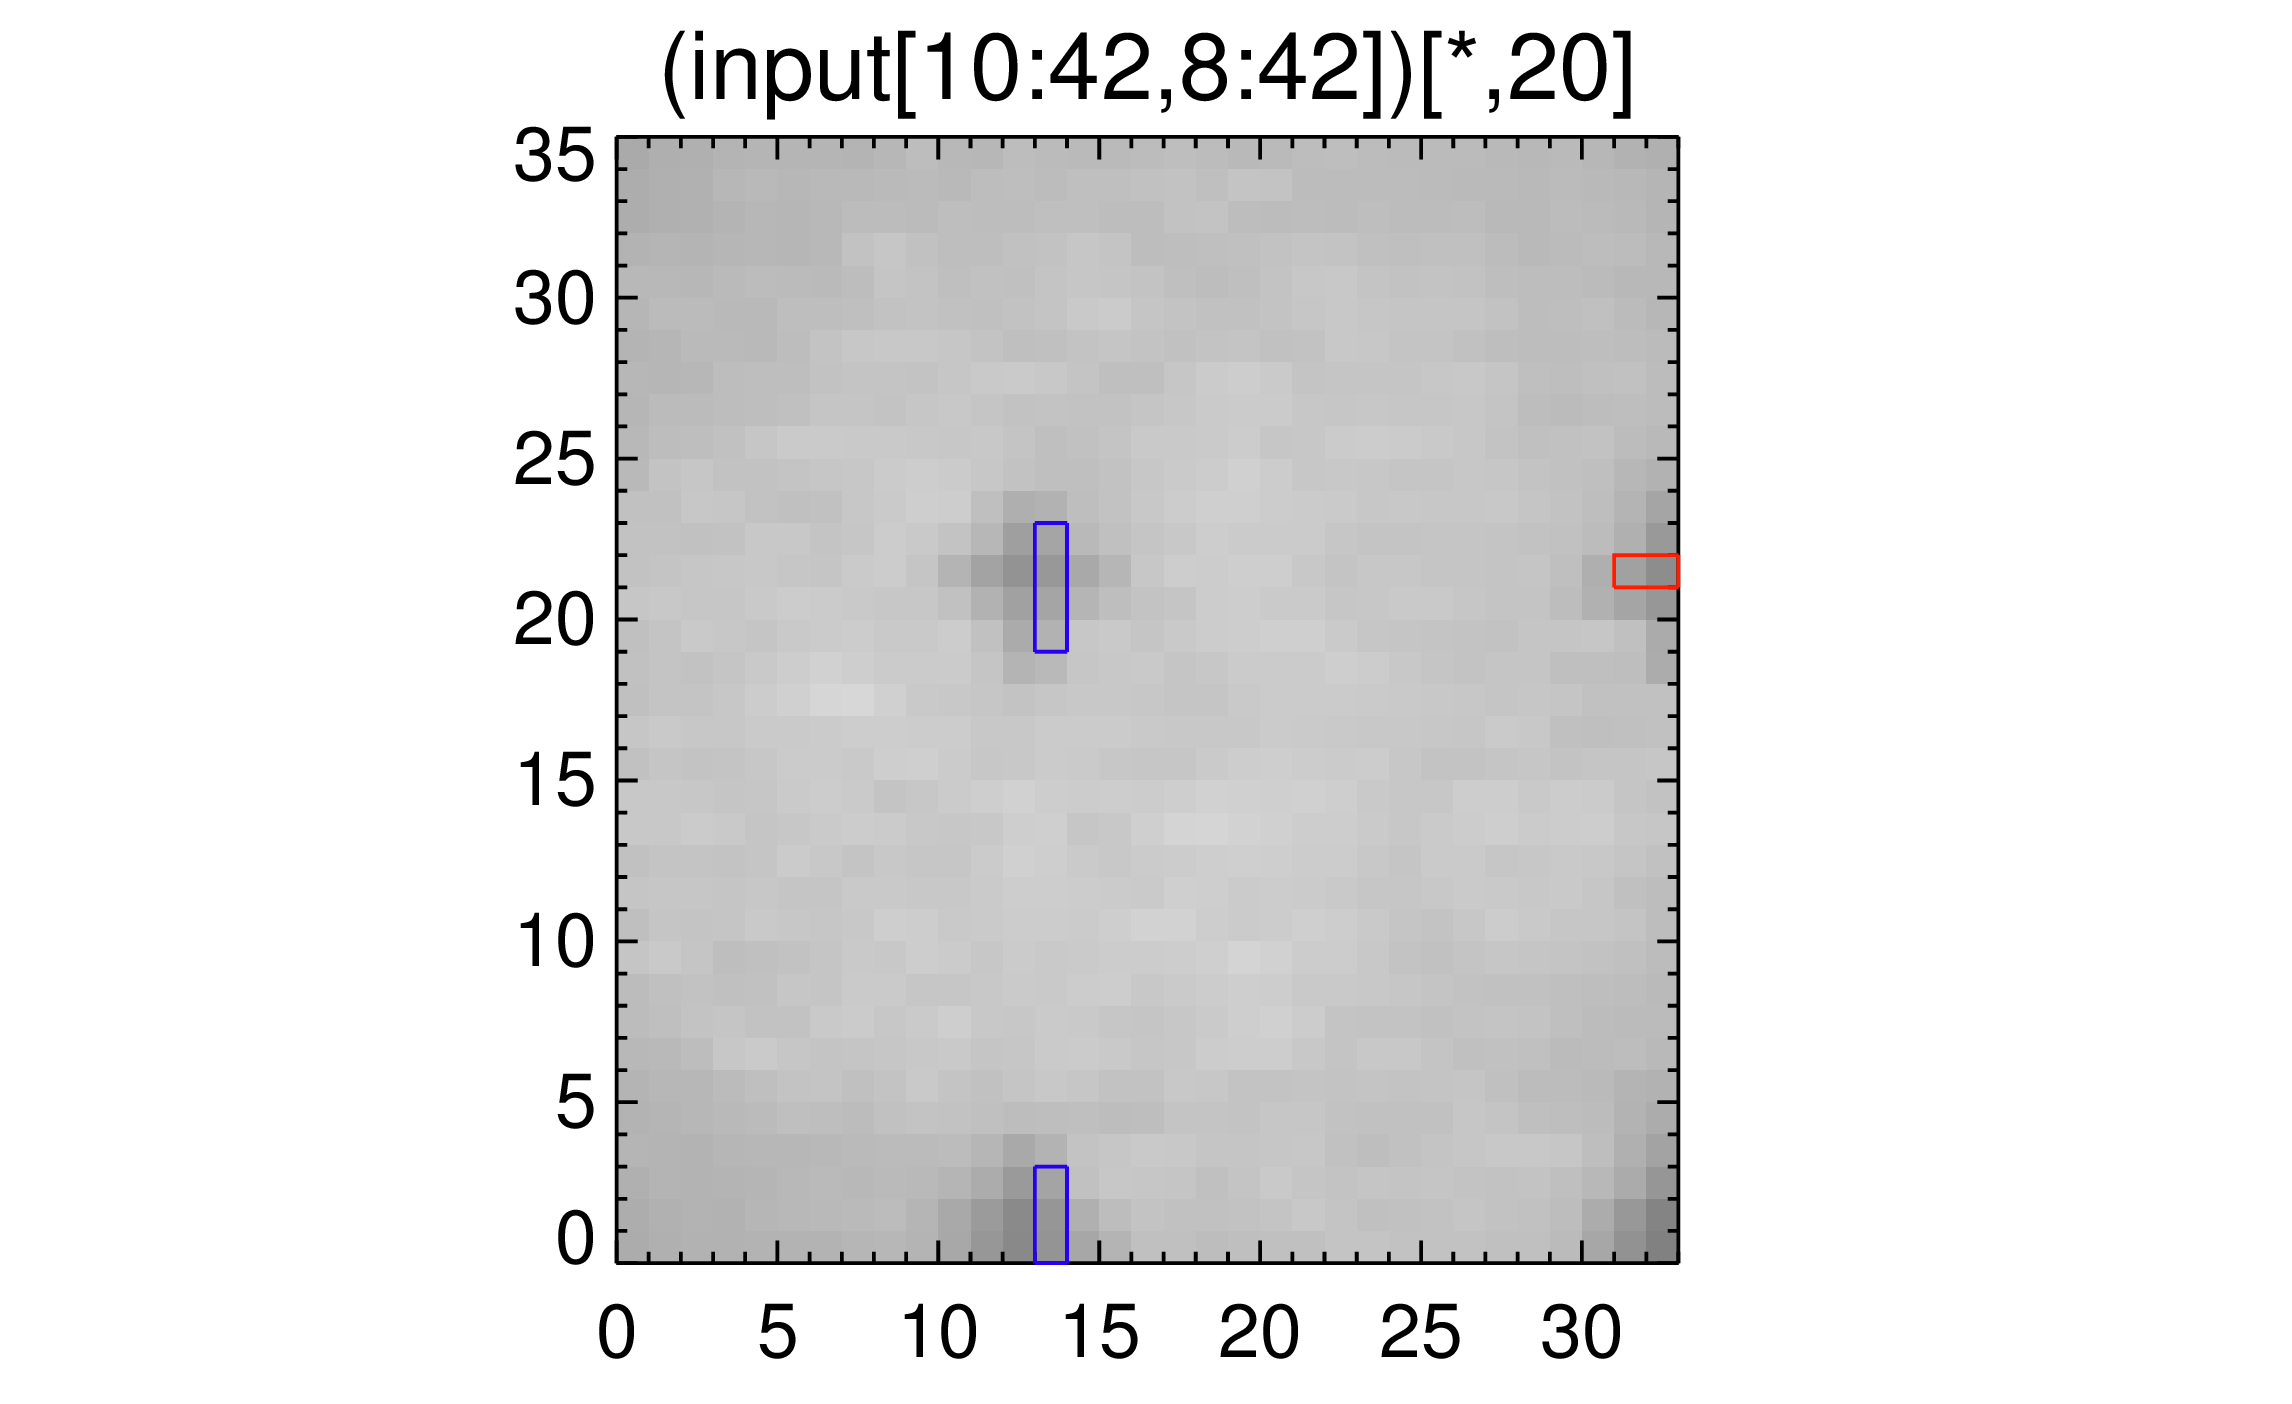
\includegraphics[width=1.3\textwidth]{../plots_tables_images/moarfidcheck_withbothtruncate4.png}
%         \caption{4 pixels}
%     \end{subfigure}

%     \begin{subfigure}[b]{.45\linewidth}
%         \centering
%         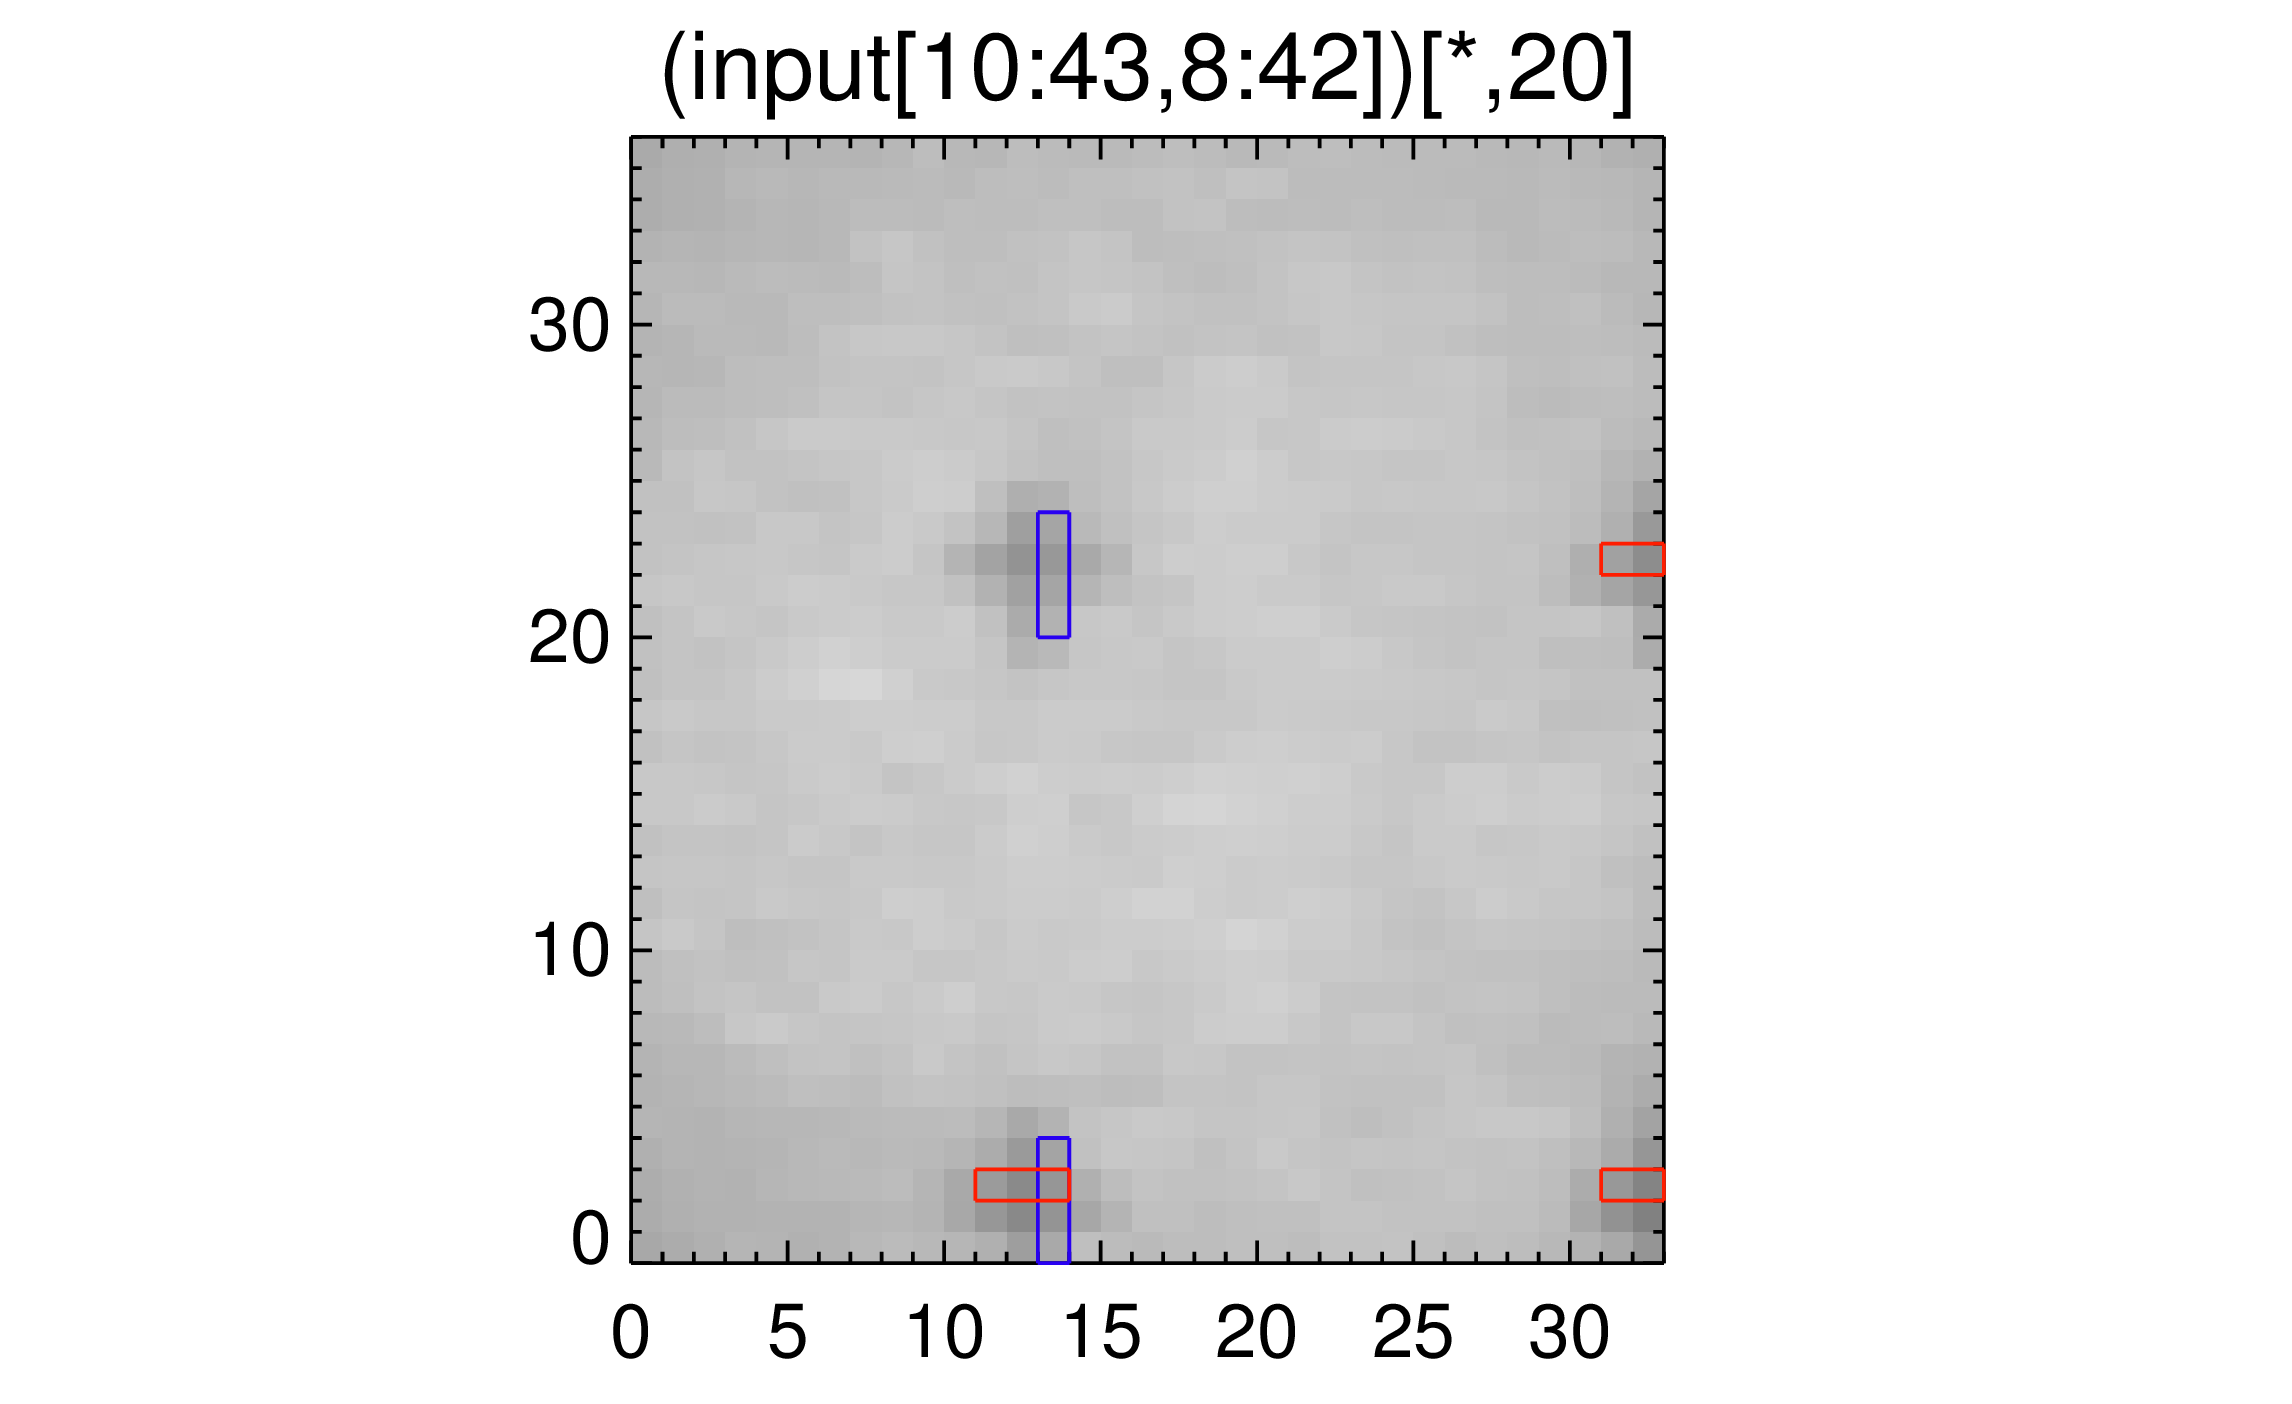
\includegraphics[width=1.3\textwidth]{../plots_tables_images/moarfidcheck_withbothtruncate5.png}
%         \caption{5 pixels}
%     \end{subfigure}
%     \begin{subfigure}[b]{.45\linewidth}
%         \centering
%         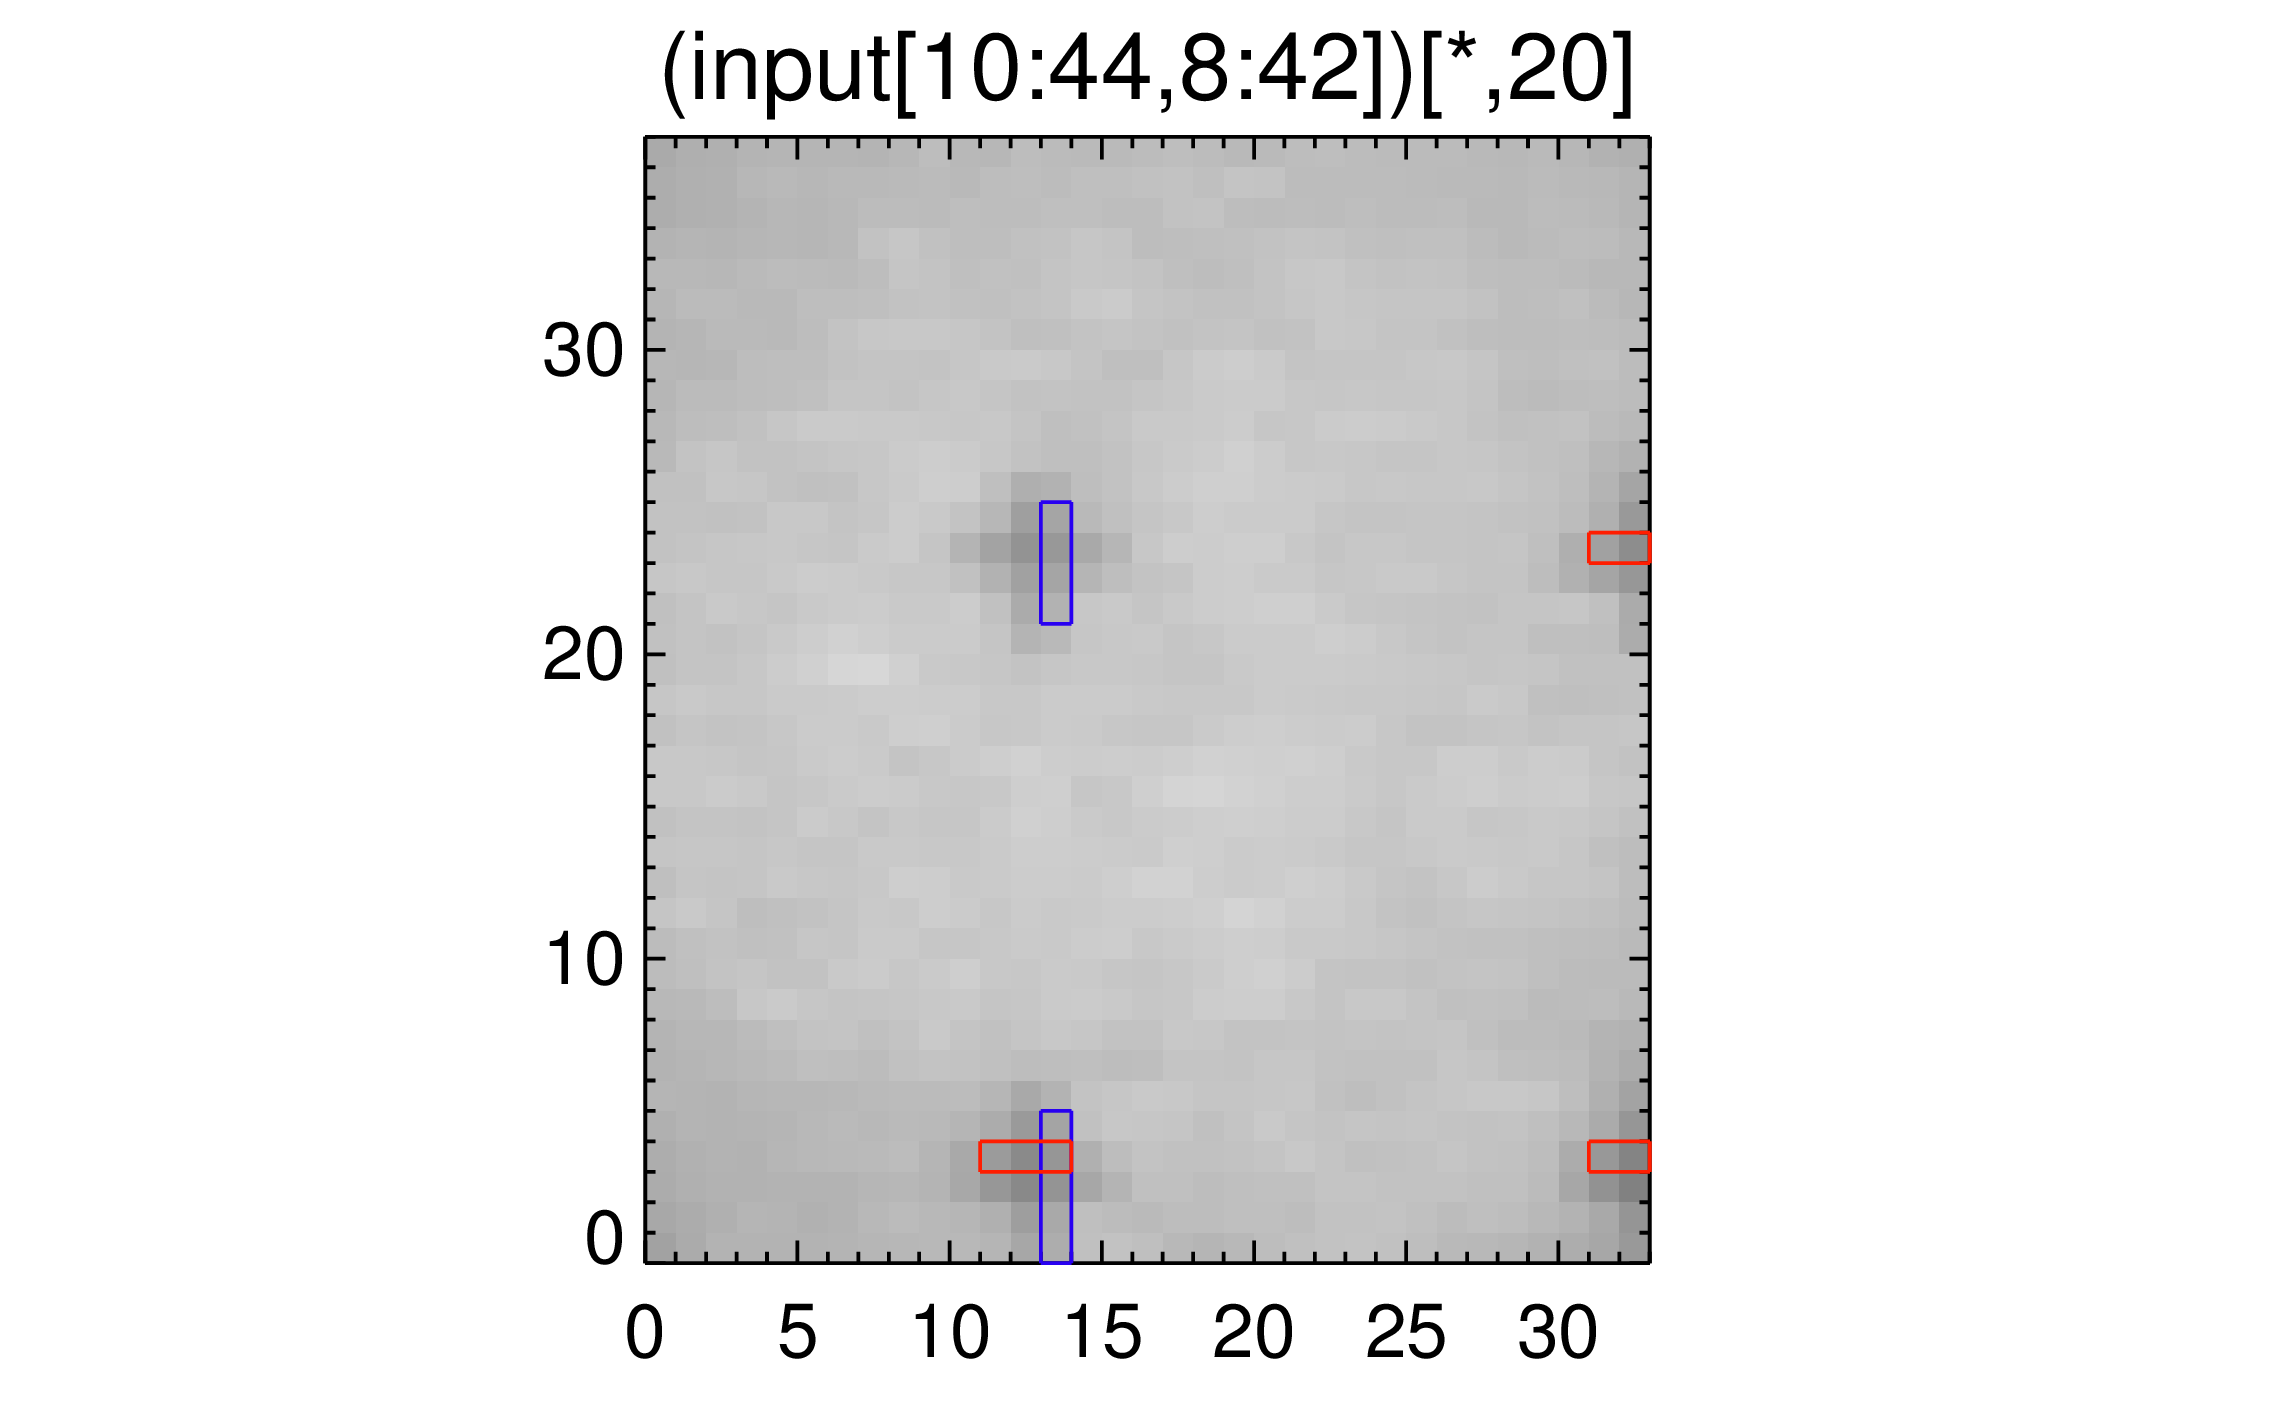
\includegraphics[width=1.3\textwidth]{../plots_tables_images/moarfidcheck_withbothtruncate6.png}
%         \caption{Completely in image}
%     \end{subfigure}
%     \caption{This time, we're cropping the bottom less and less}
%     \label{firstplot}
% \end{figure}

% subsection another_example_of_filters_on_an_increasingly_cropped_image (end)

\subsection{Changing direction of edge filters} % (fold)
\label{sub:changing_direction_of_edge_filters}


I thought perhaps the direction in which we were cropping and the location of where the filters identified had the fiducial had an effect on our threshold of ``how-bad-can-it-get''. To test this, I shifted the filters 180$^\circ$ to instead find an edge somewhere else in the fiducual. To be clear, to find an x-position of a fiducial we ran filters in the x direction to isolate the blue-outlined pixels. These positions are consistently the right 2 pixels of the fiducial's 2x2 center. If the edge detected are on the right and we're cropping the right of the image off, there's a chance that we're cropping off that detected edge 1 pixel early, so I modified the code so that it find the left 2 pixels of the center 2x2 so hopefully the fiducial could be more cut off and we'd still get fiducial positions. Results are shown in Figure \ref{isitok}.

\begin{figure}[!ht]
    \ffigbox[][\FBheight]{%
    \begin{subfloatrow}[2]%
        \ffigbox[\FBwidth]%
       {%
       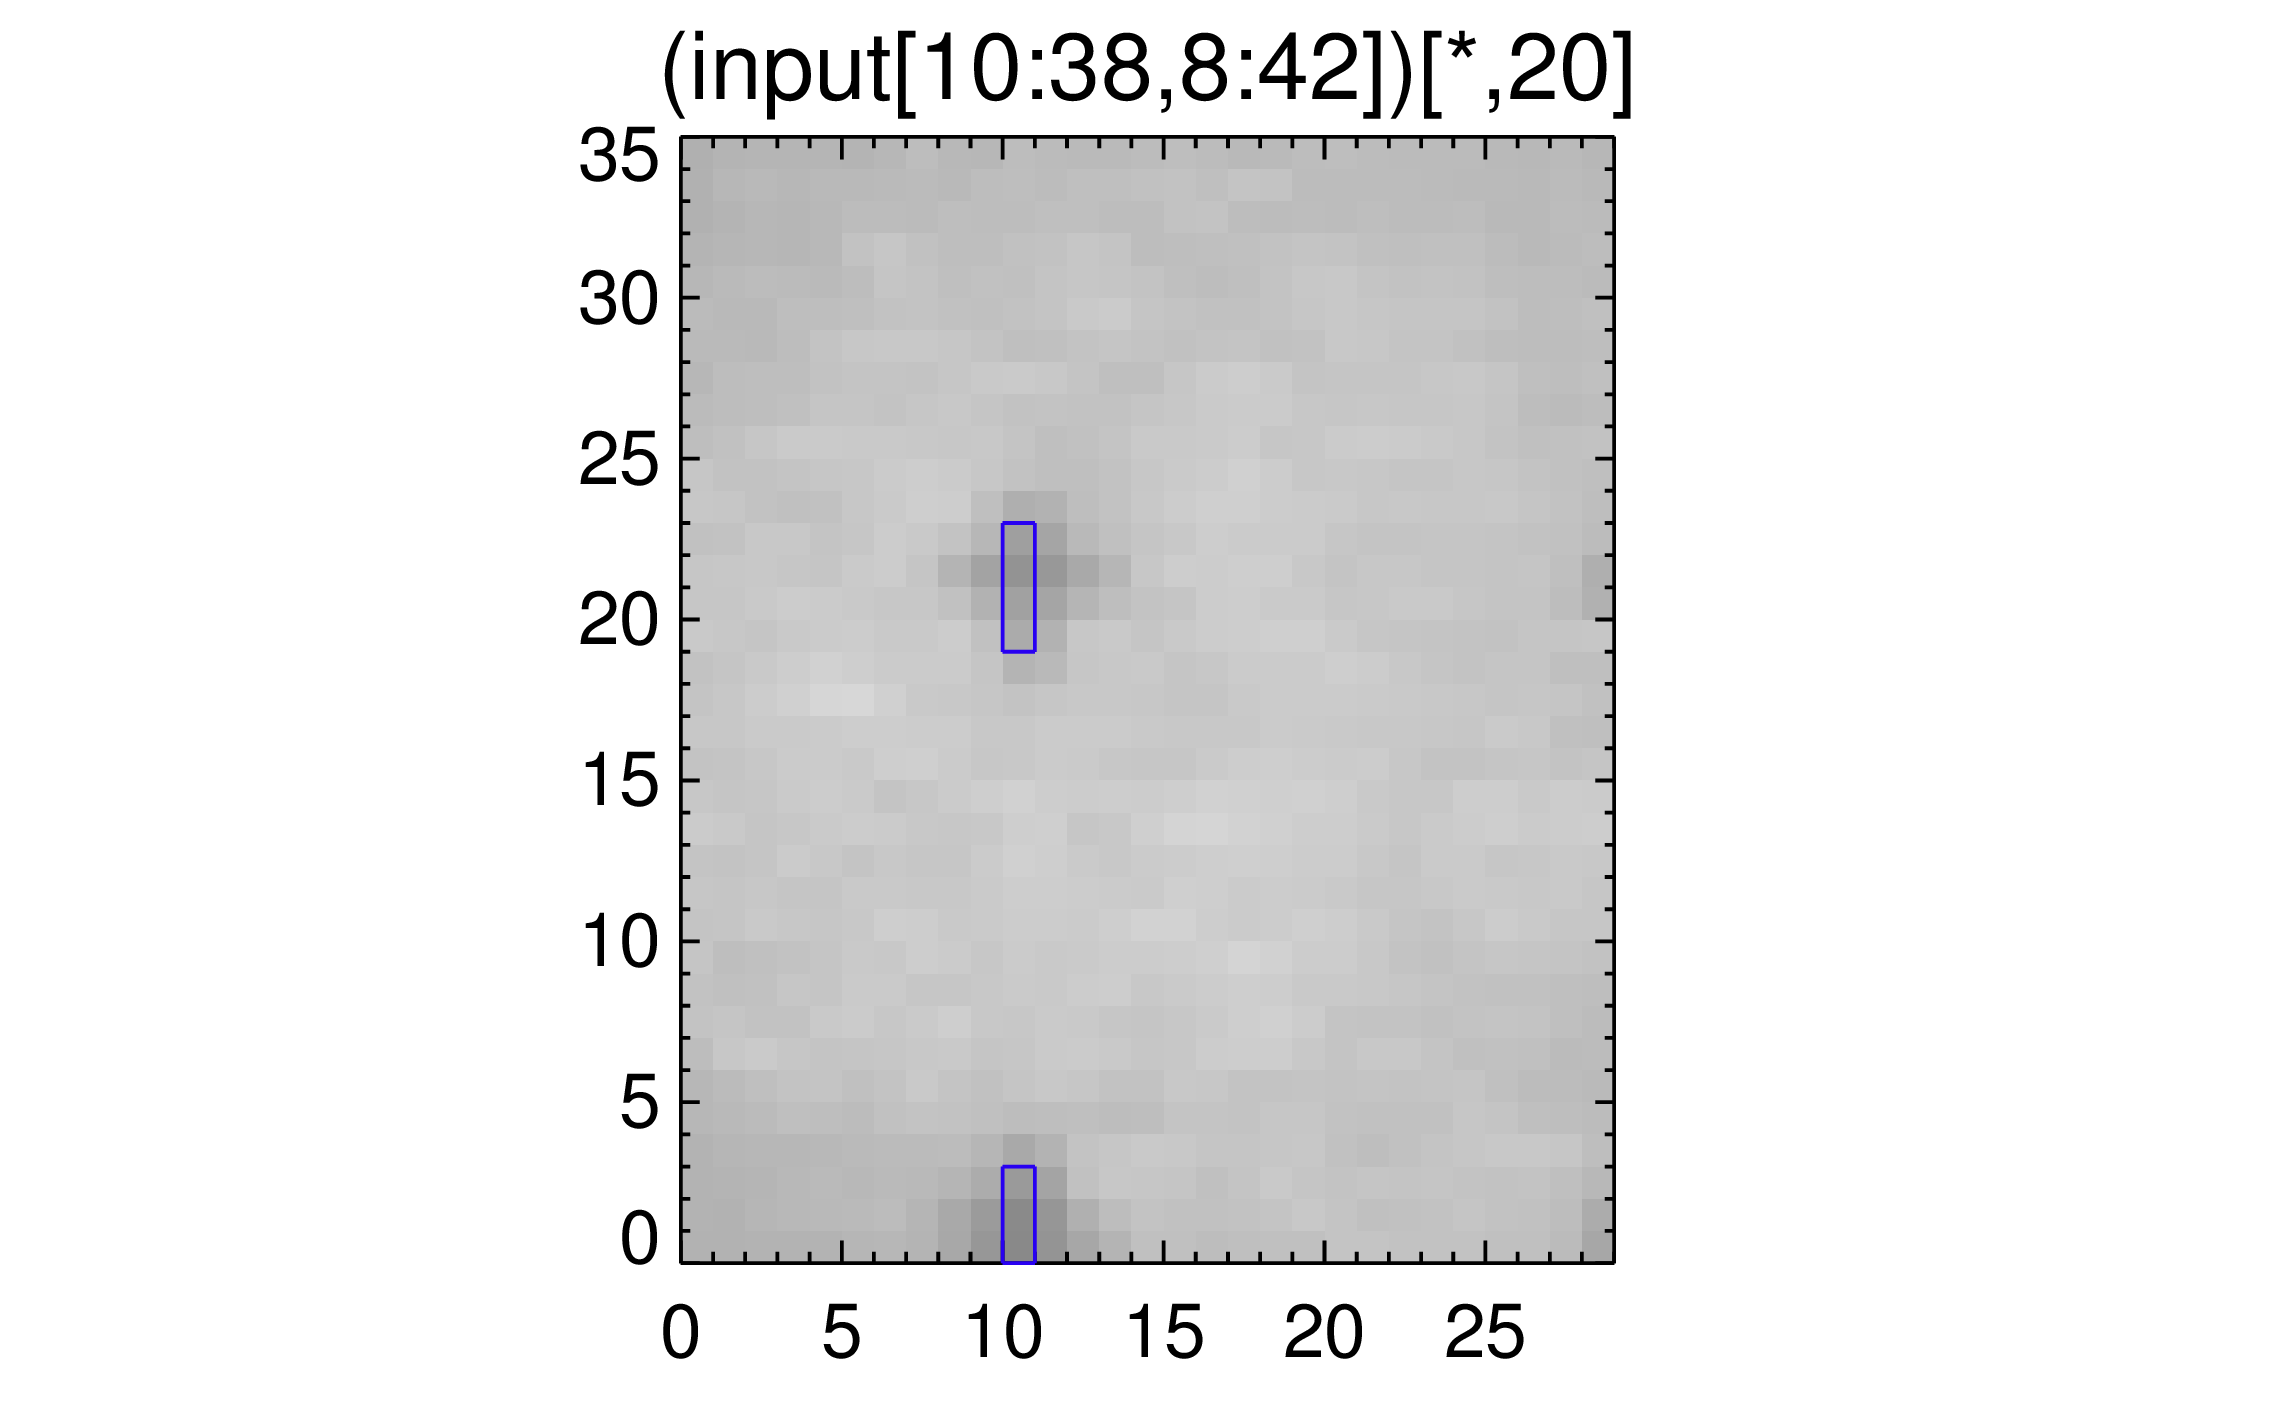
\includegraphics[width=.5\textwidth]{../plots_tables_images/fidcheck_newdegree0.png}%
       }%
       {%
       \caption{1 Fiducial pixel in image}%
       }%
        \ffigbox[\Xhsize]%
       {%
       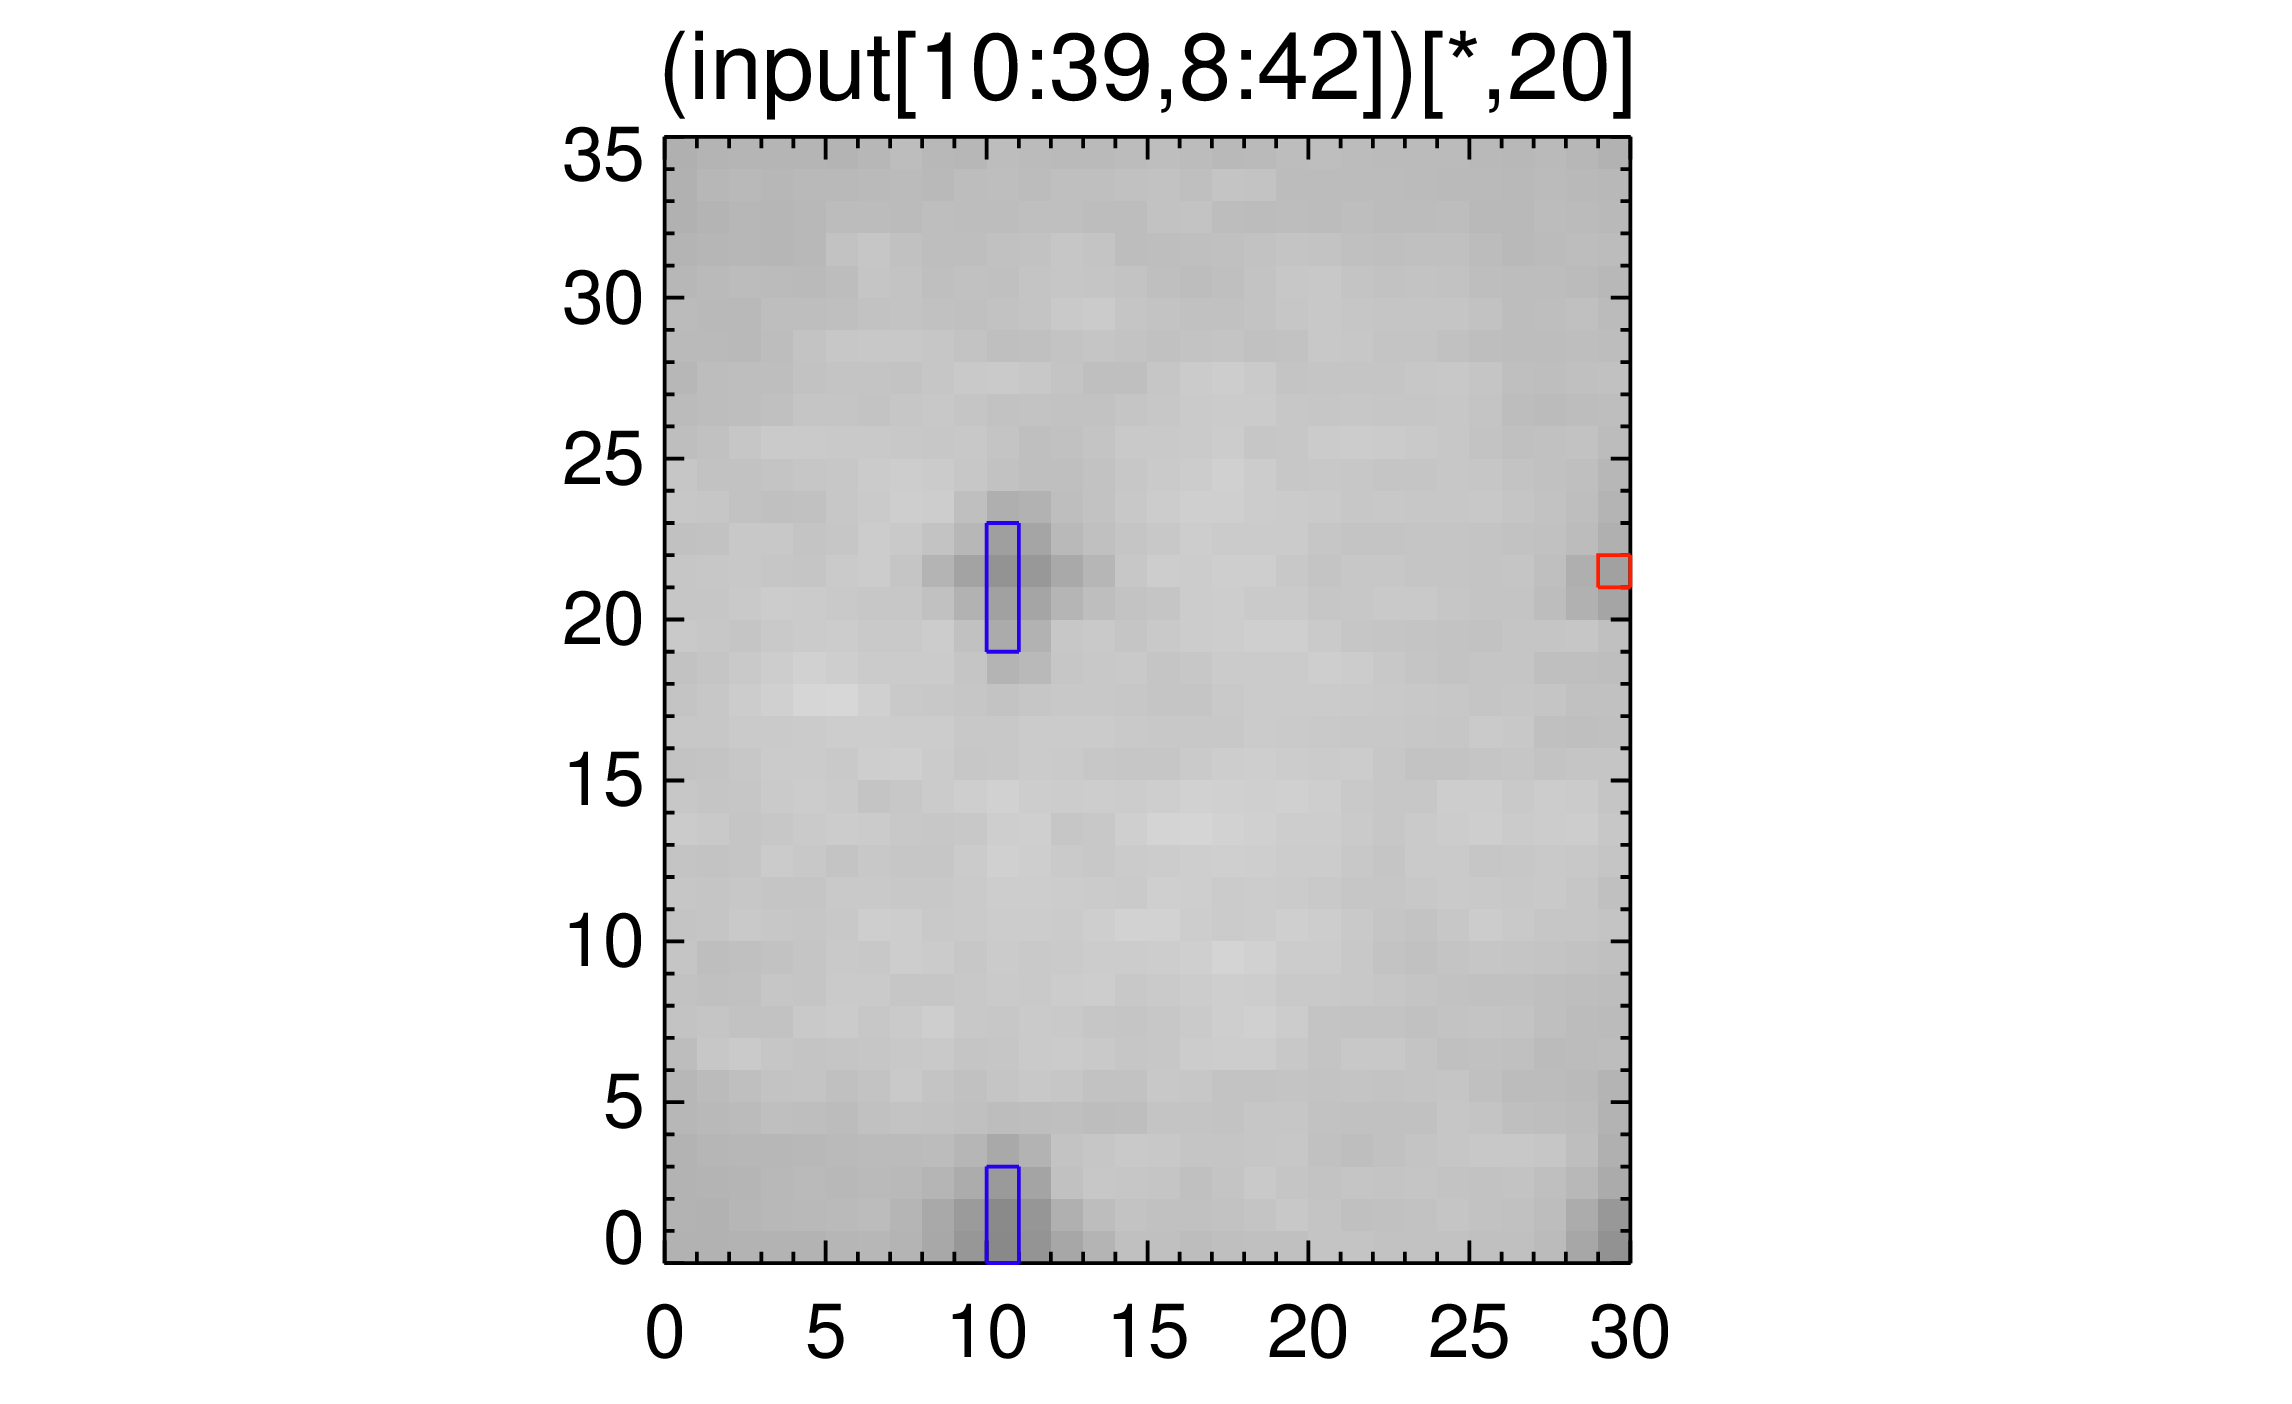
\includegraphics[width=.5\textwidth]{../plots_tables_images/fidcheck_newdegree1.png}%
       }%
       {%
       \caption{2 pixels}%
       }%
    \end{subfloatrow}}

    \ffigbox[][\FBheight]{%
    \begin{subfloatrow}[2]%
        \ffigbox[\FBwidth]%
       {%
       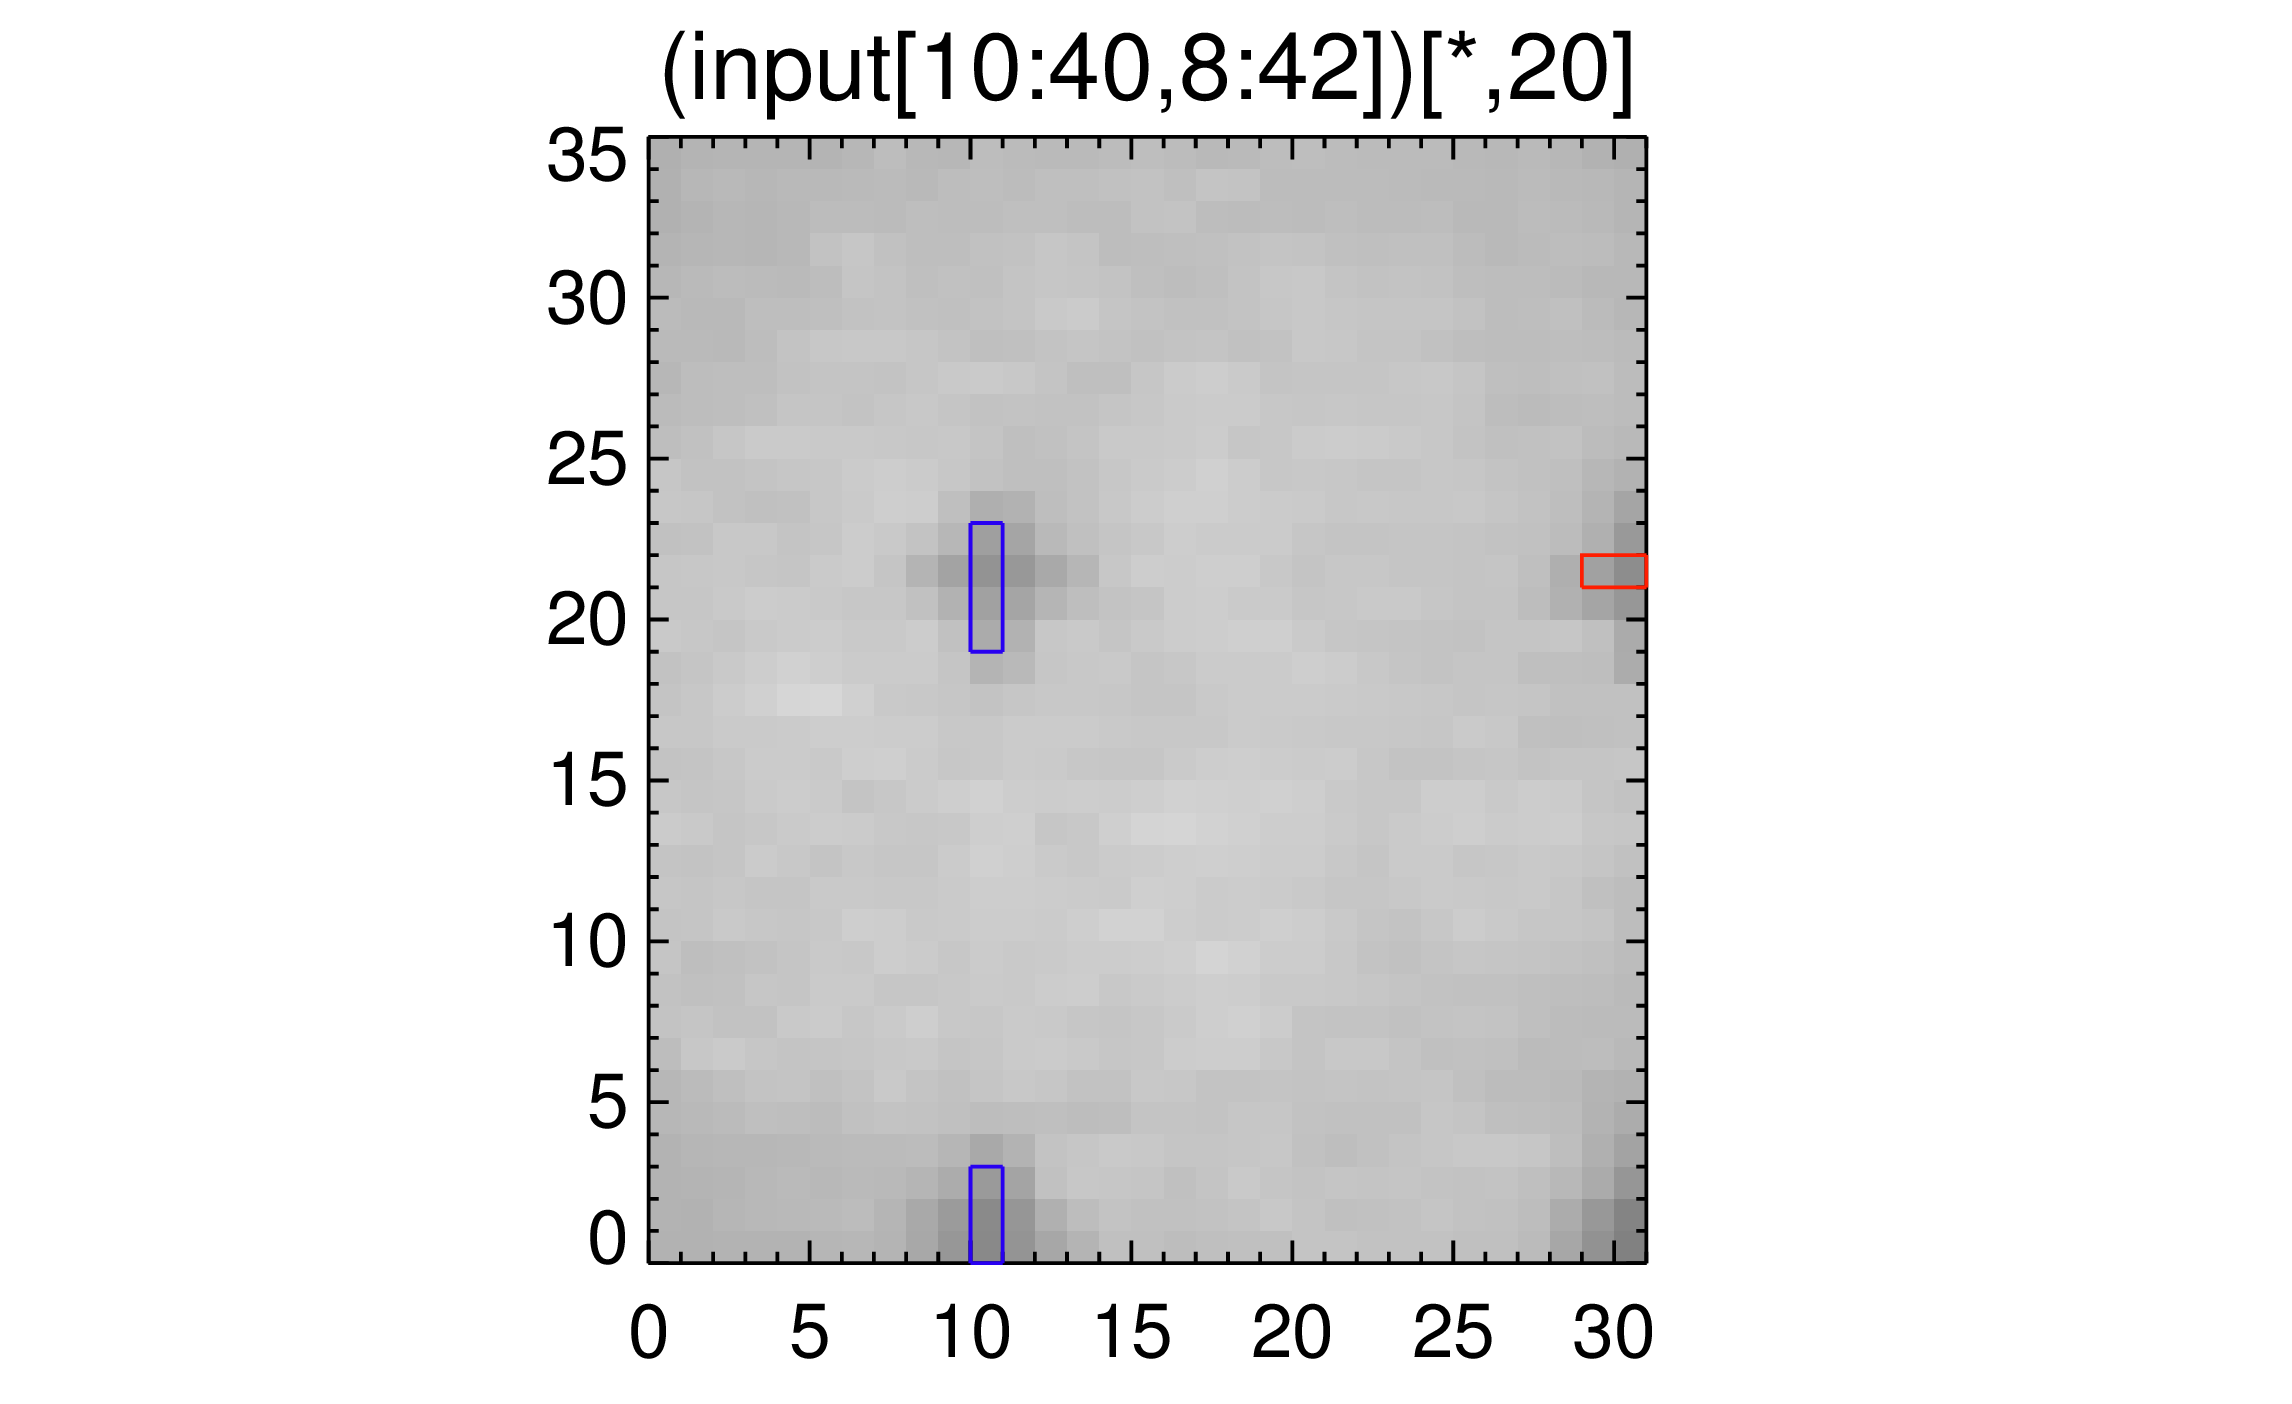
\includegraphics[width=.5\textwidth]{../plots_tables_images/fidcheck_newdegree2.png}%
       }%
       {%
       \caption{3 pixels}%
       }%
        \ffigbox[\Xhsize]%
       {%
       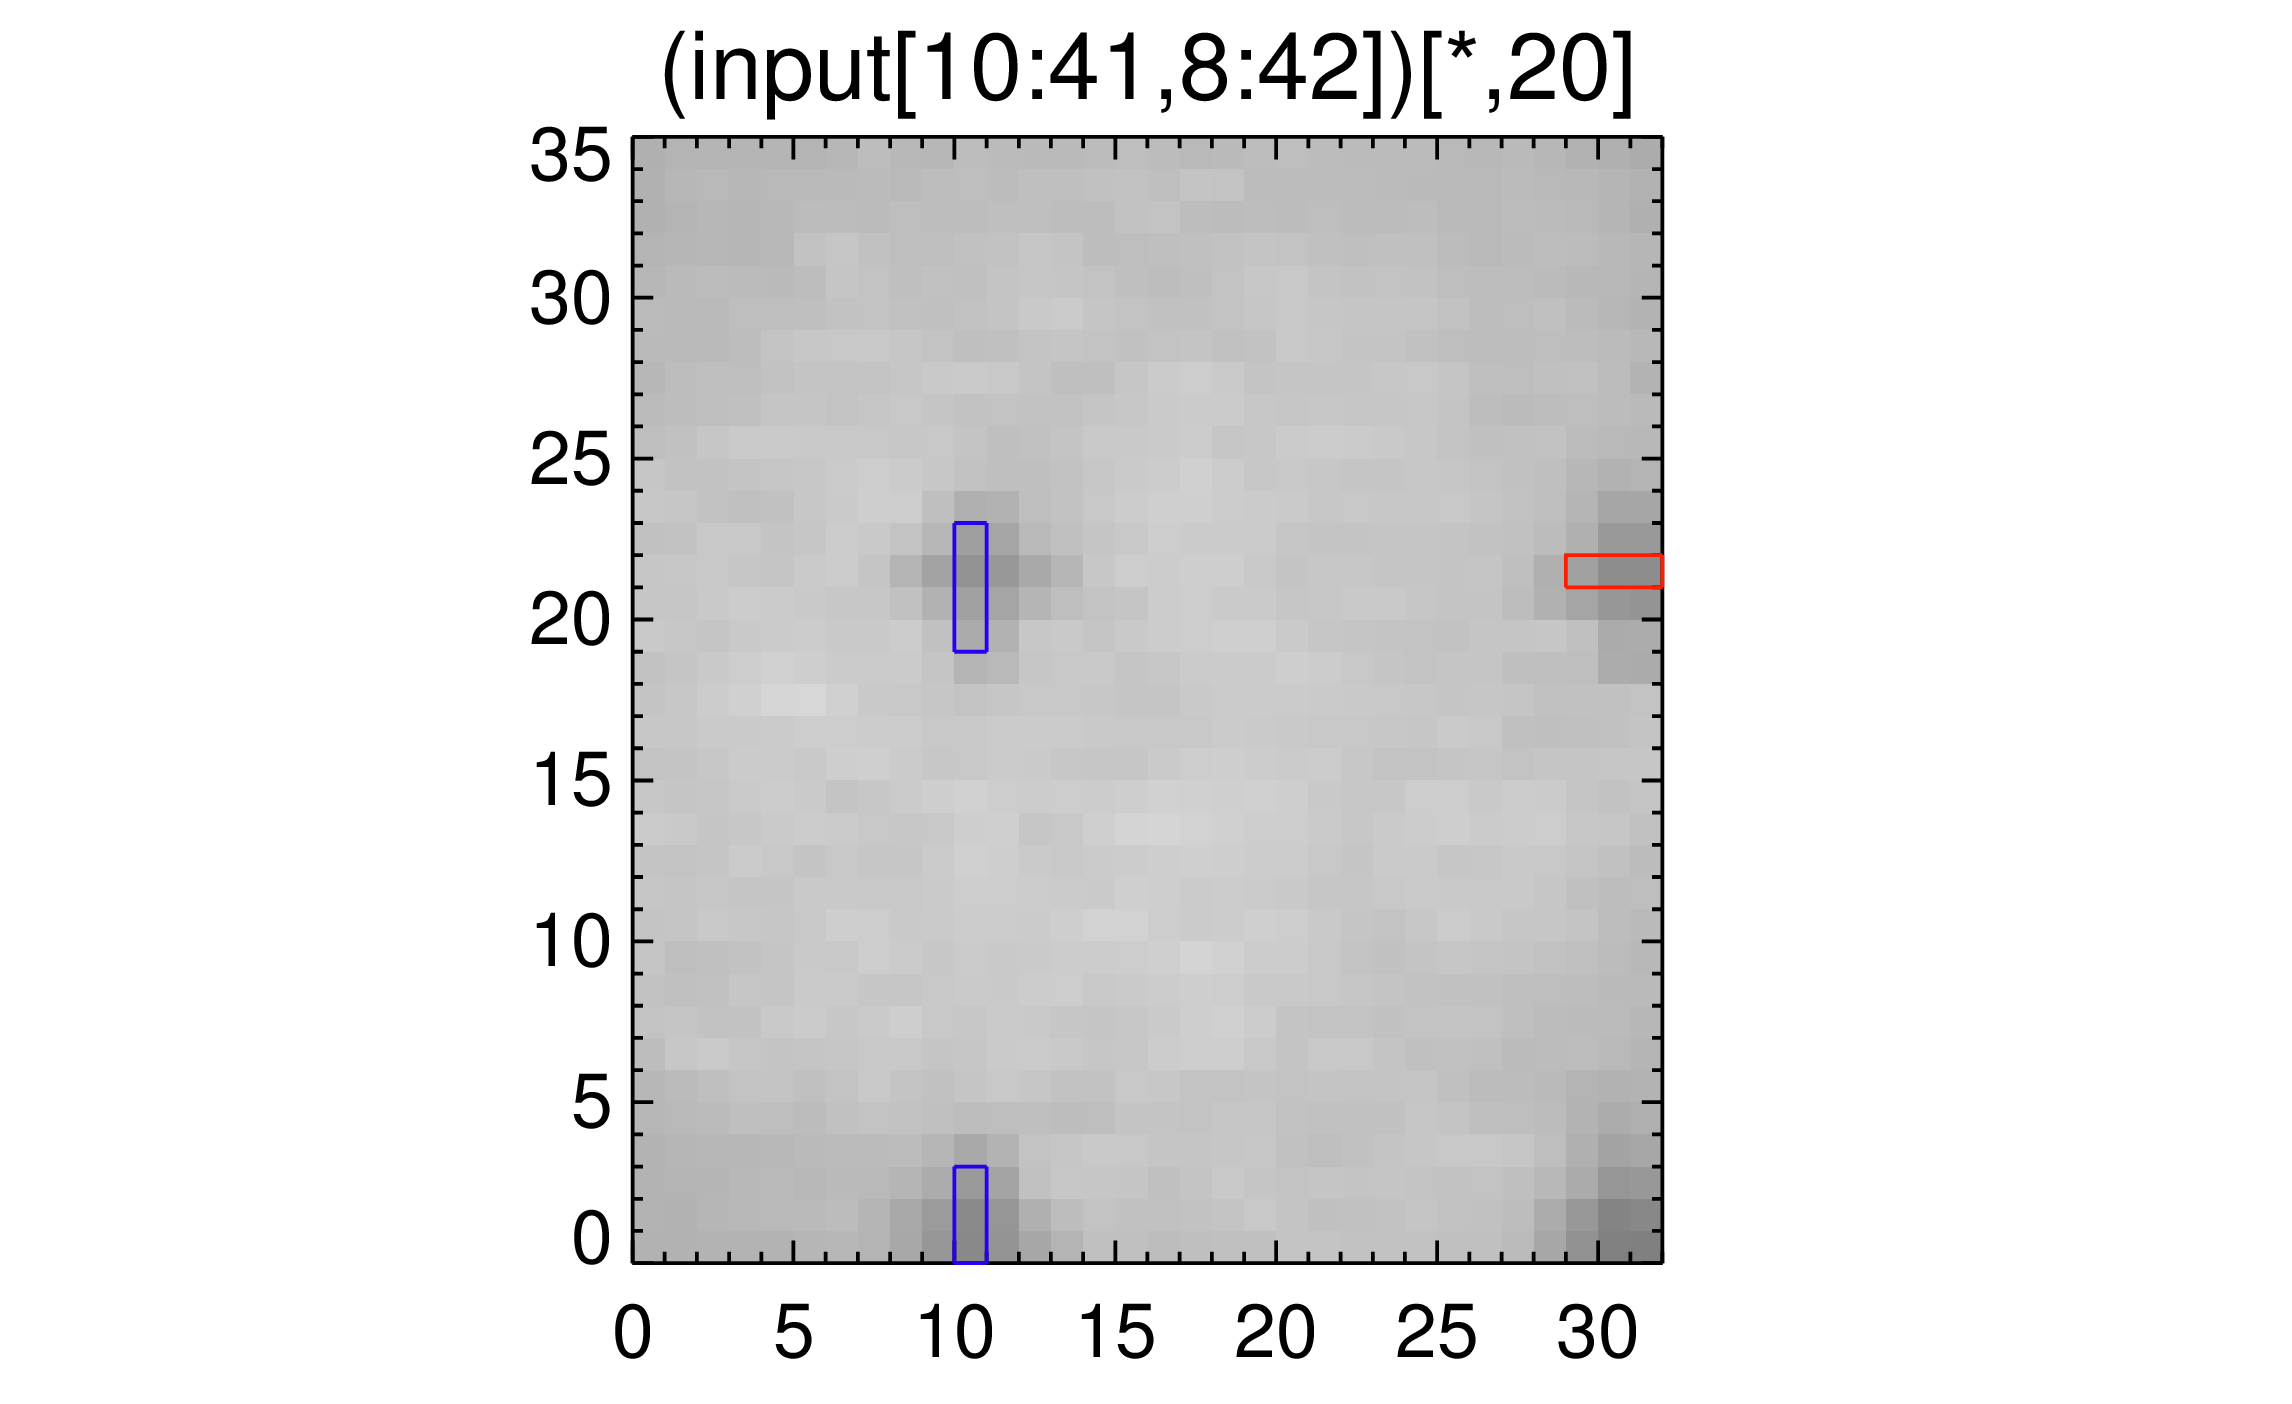
\includegraphics[width=.5\textwidth]{../plots_tables_images/fidcheck_newdegree3.png}%
       }%
       {%
       \caption{4 pixels}%
       }%
    \end{subfloatrow}}

    \ffigbox[][\FBheight]{%
    \begin{subfloatrow}[2]%
        \ffigbox[\FBwidth]%
       {%
       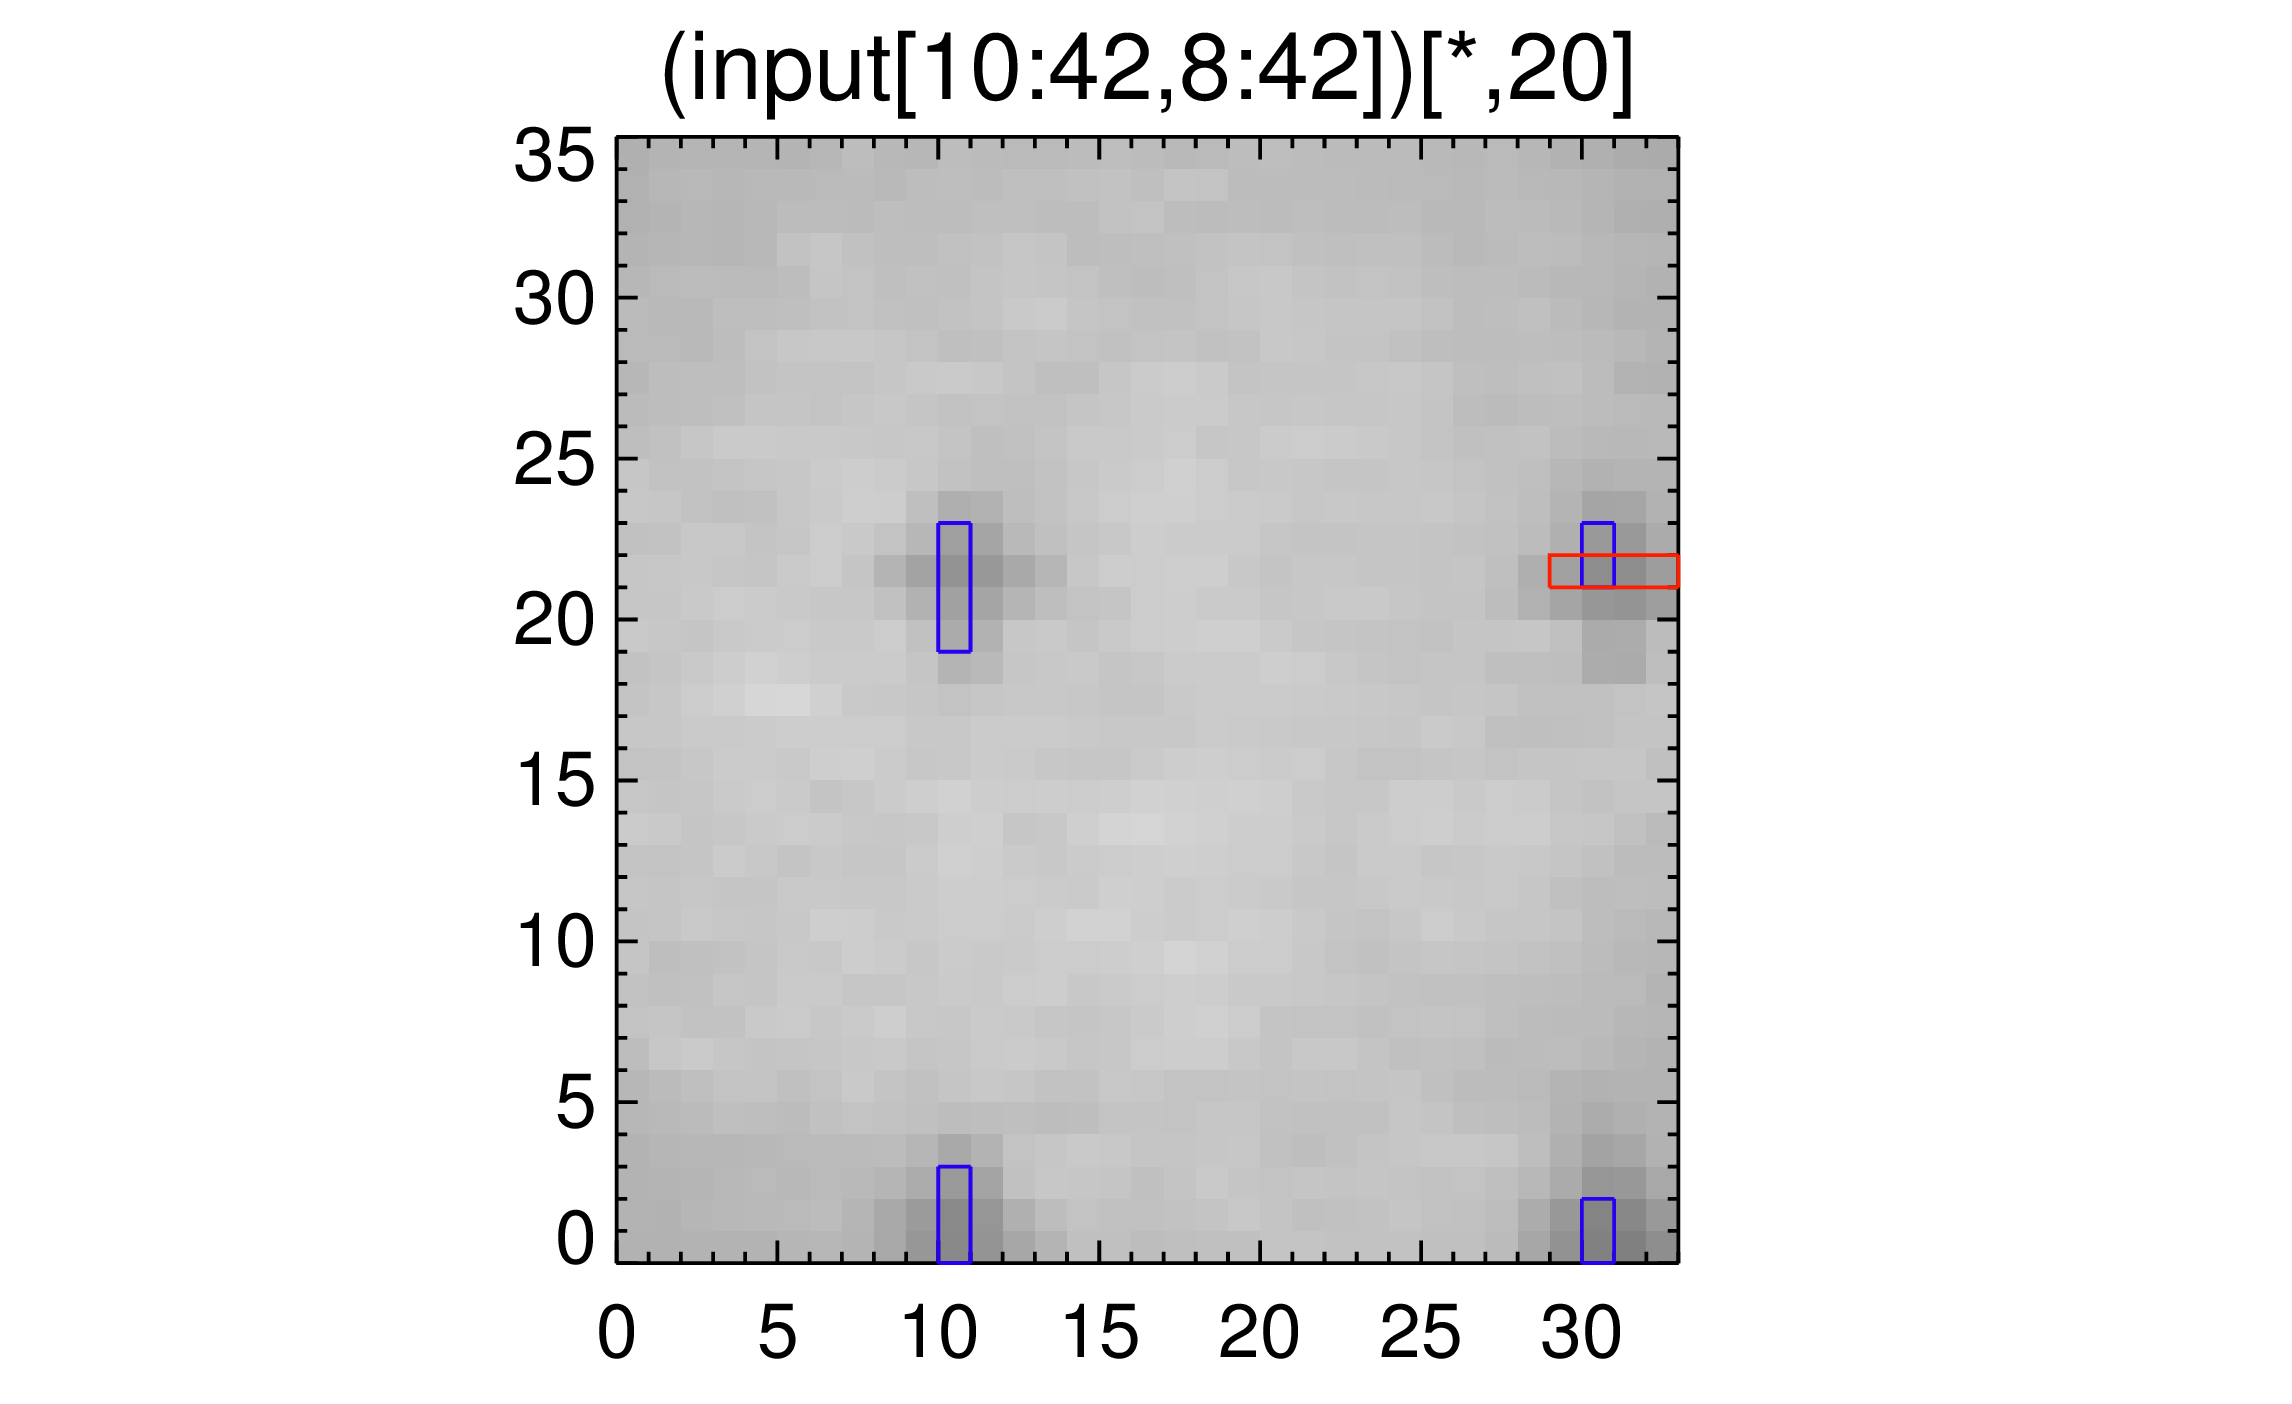
\includegraphics[width=.5\textwidth]{../plots_tables_images/fidcheck_newdegree4.png}%
       }%
       {%
       \caption{5 pixels}%
       }%
        \ffigbox[\Xhsize]%
       {%
       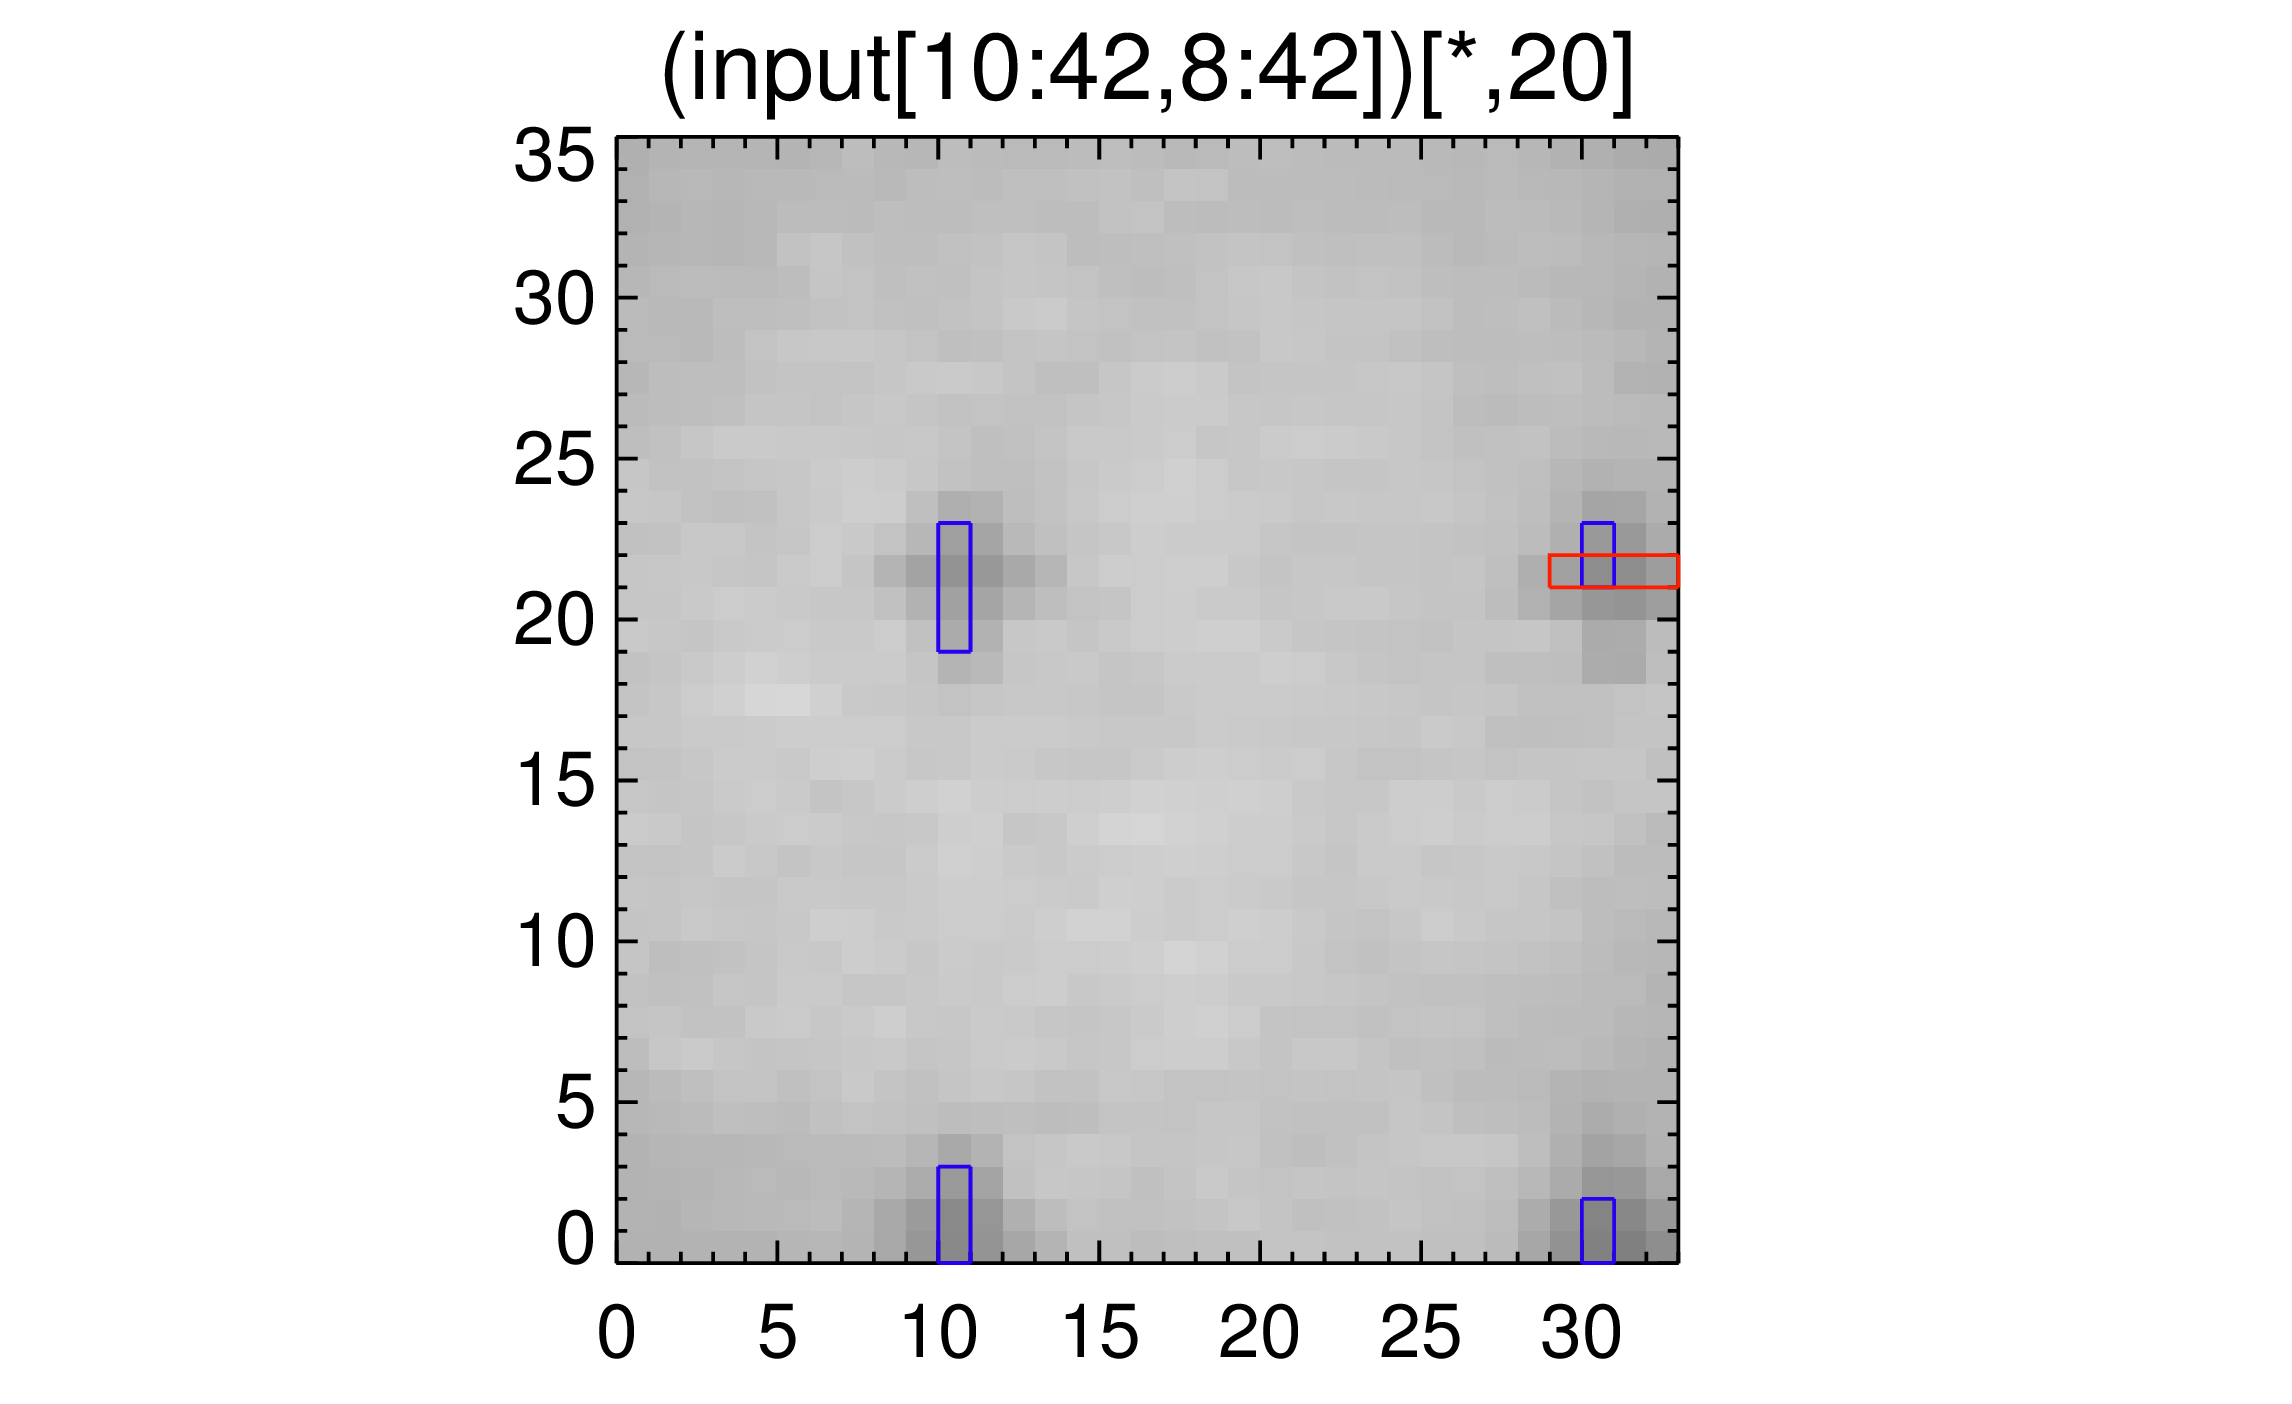
\includegraphics[width=.5\textwidth]{../plots_tables_images/fidcheck_newdegree4.png}%
       }%
       {%
       \caption{Completely in image}%
       }%
    \end{subfloatrow}}{\caption{Finding the left edge of the fiducual now, instead of the right edge of the fiducial}\label{isitok}}
\end{figure}

% \begin{figure}[!h]
%     \centering 
%     \begin{subfigure}[b]{.45\linewidth}
%         \centering
%         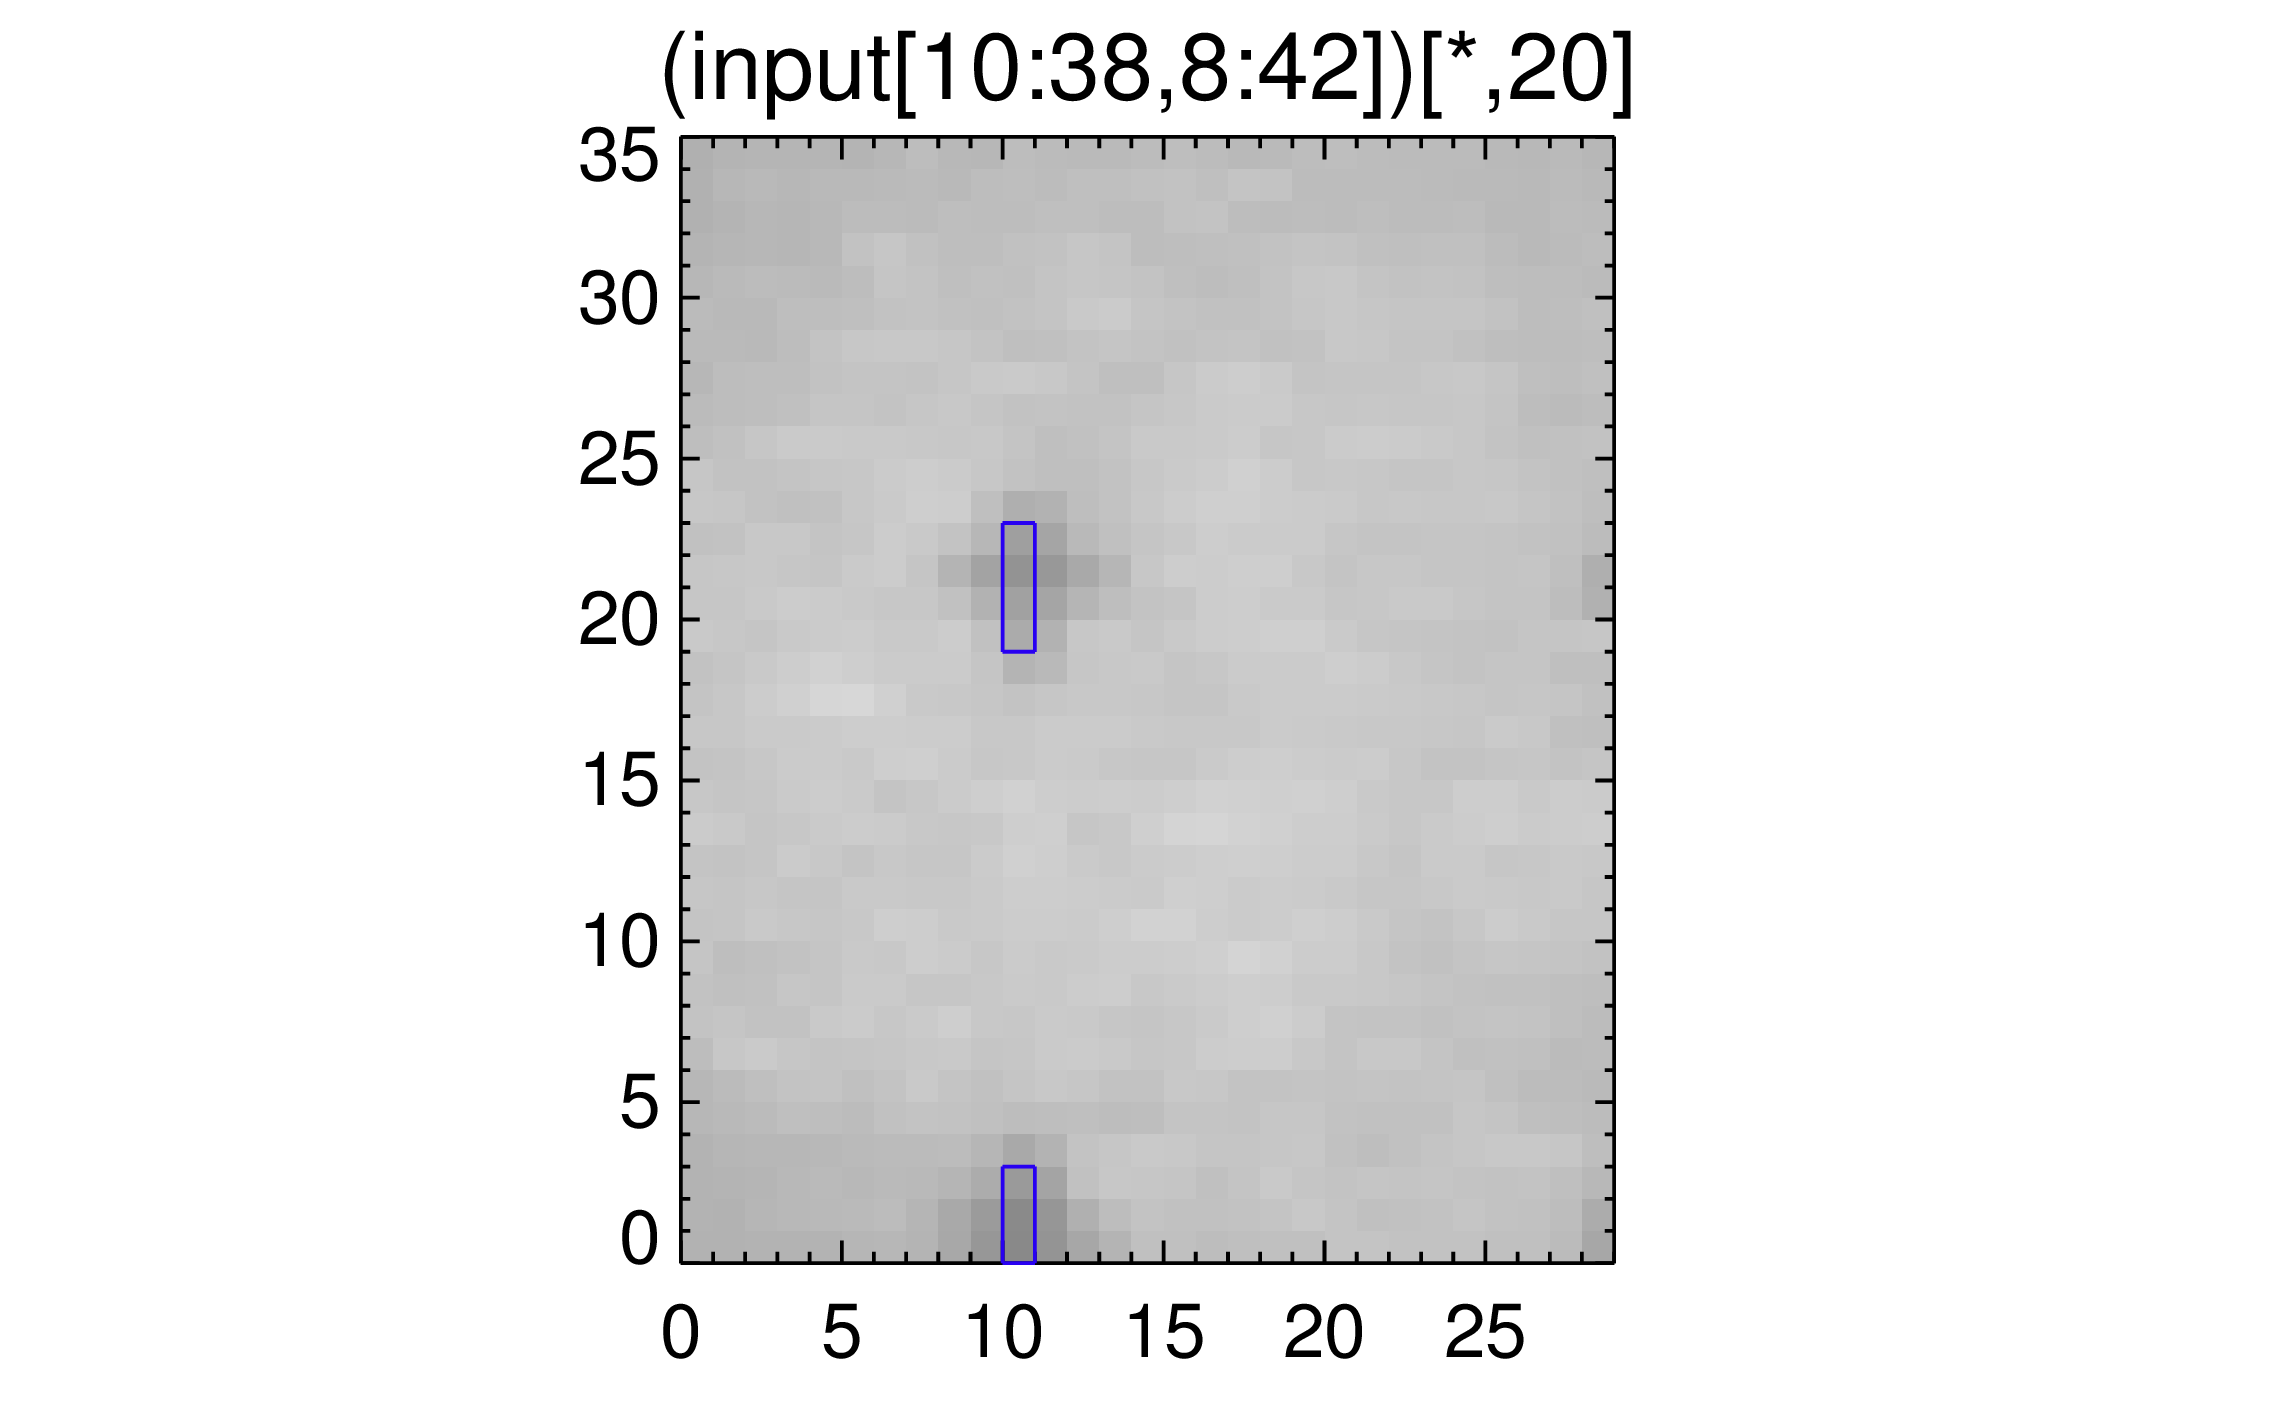
\includegraphics[width=1.3\textwidth]{../plots_tables_images/fidcheck_newdegree0.png}
%         \caption{1 Fiducial pixel in image}
%     \end{subfigure}
%     \begin{subfigure}[b]{.45\linewidth}
%         \centering
%         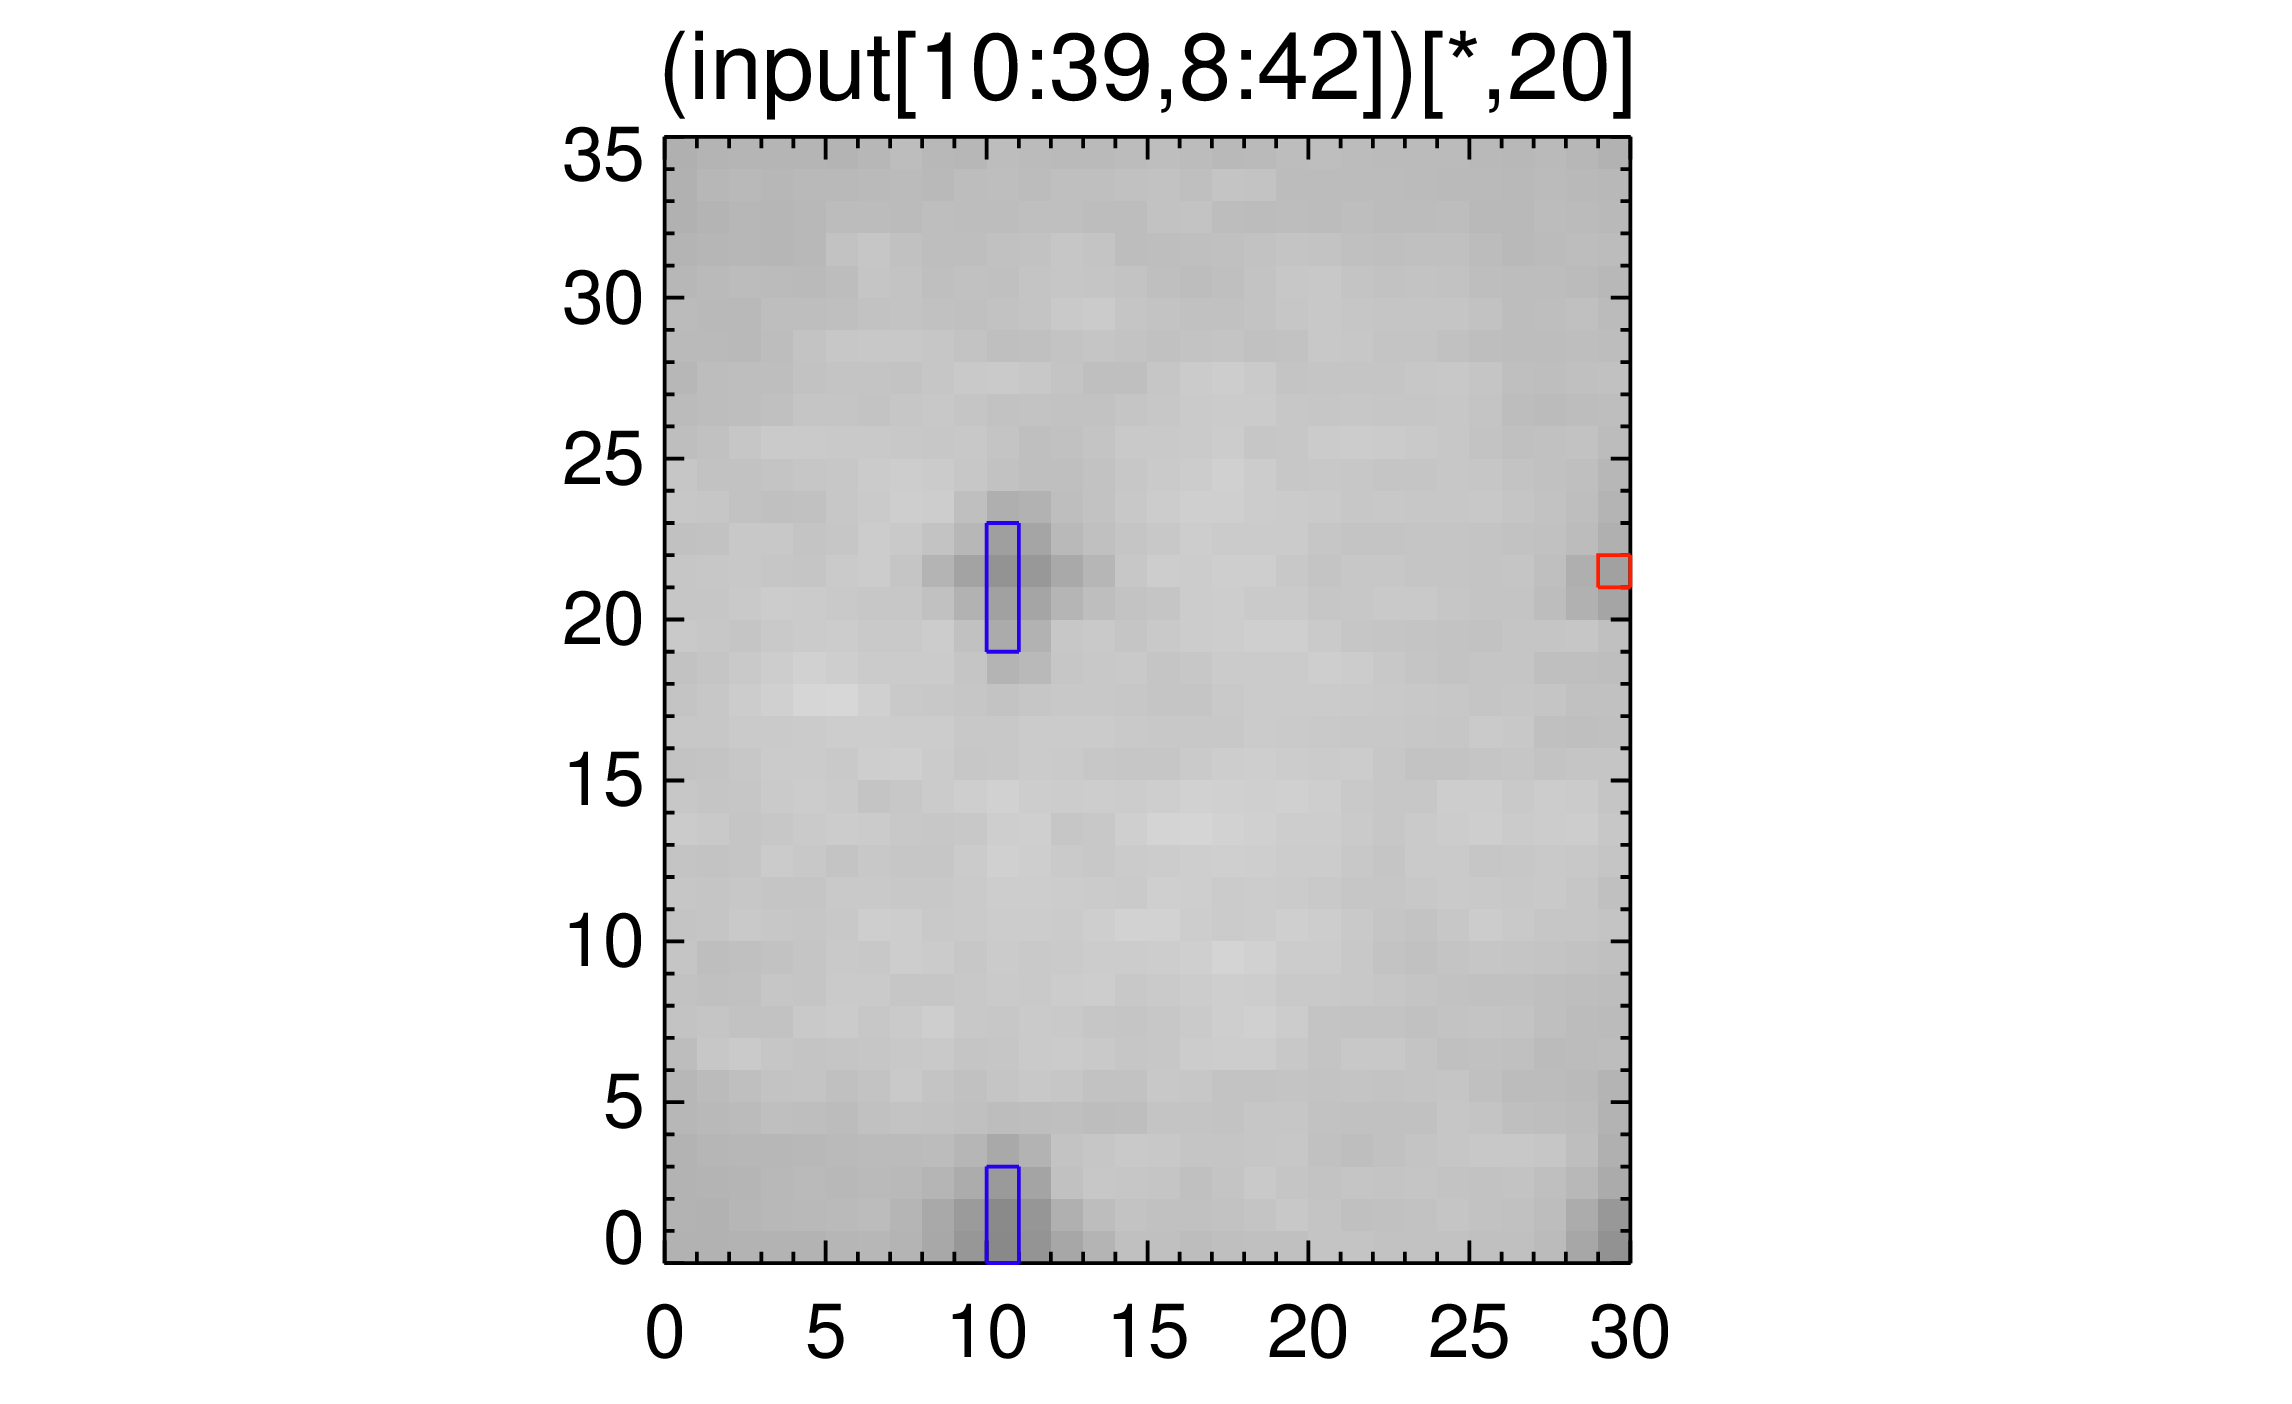
\includegraphics[width=1.3\textwidth]{../plots_tables_images/fidcheck_newdegree1.png}
%         \caption{2 pixels}
%     \end{subfigure}
   
%    \begin{subfigure}[b]{.45\linewidth}
%         \centering
%         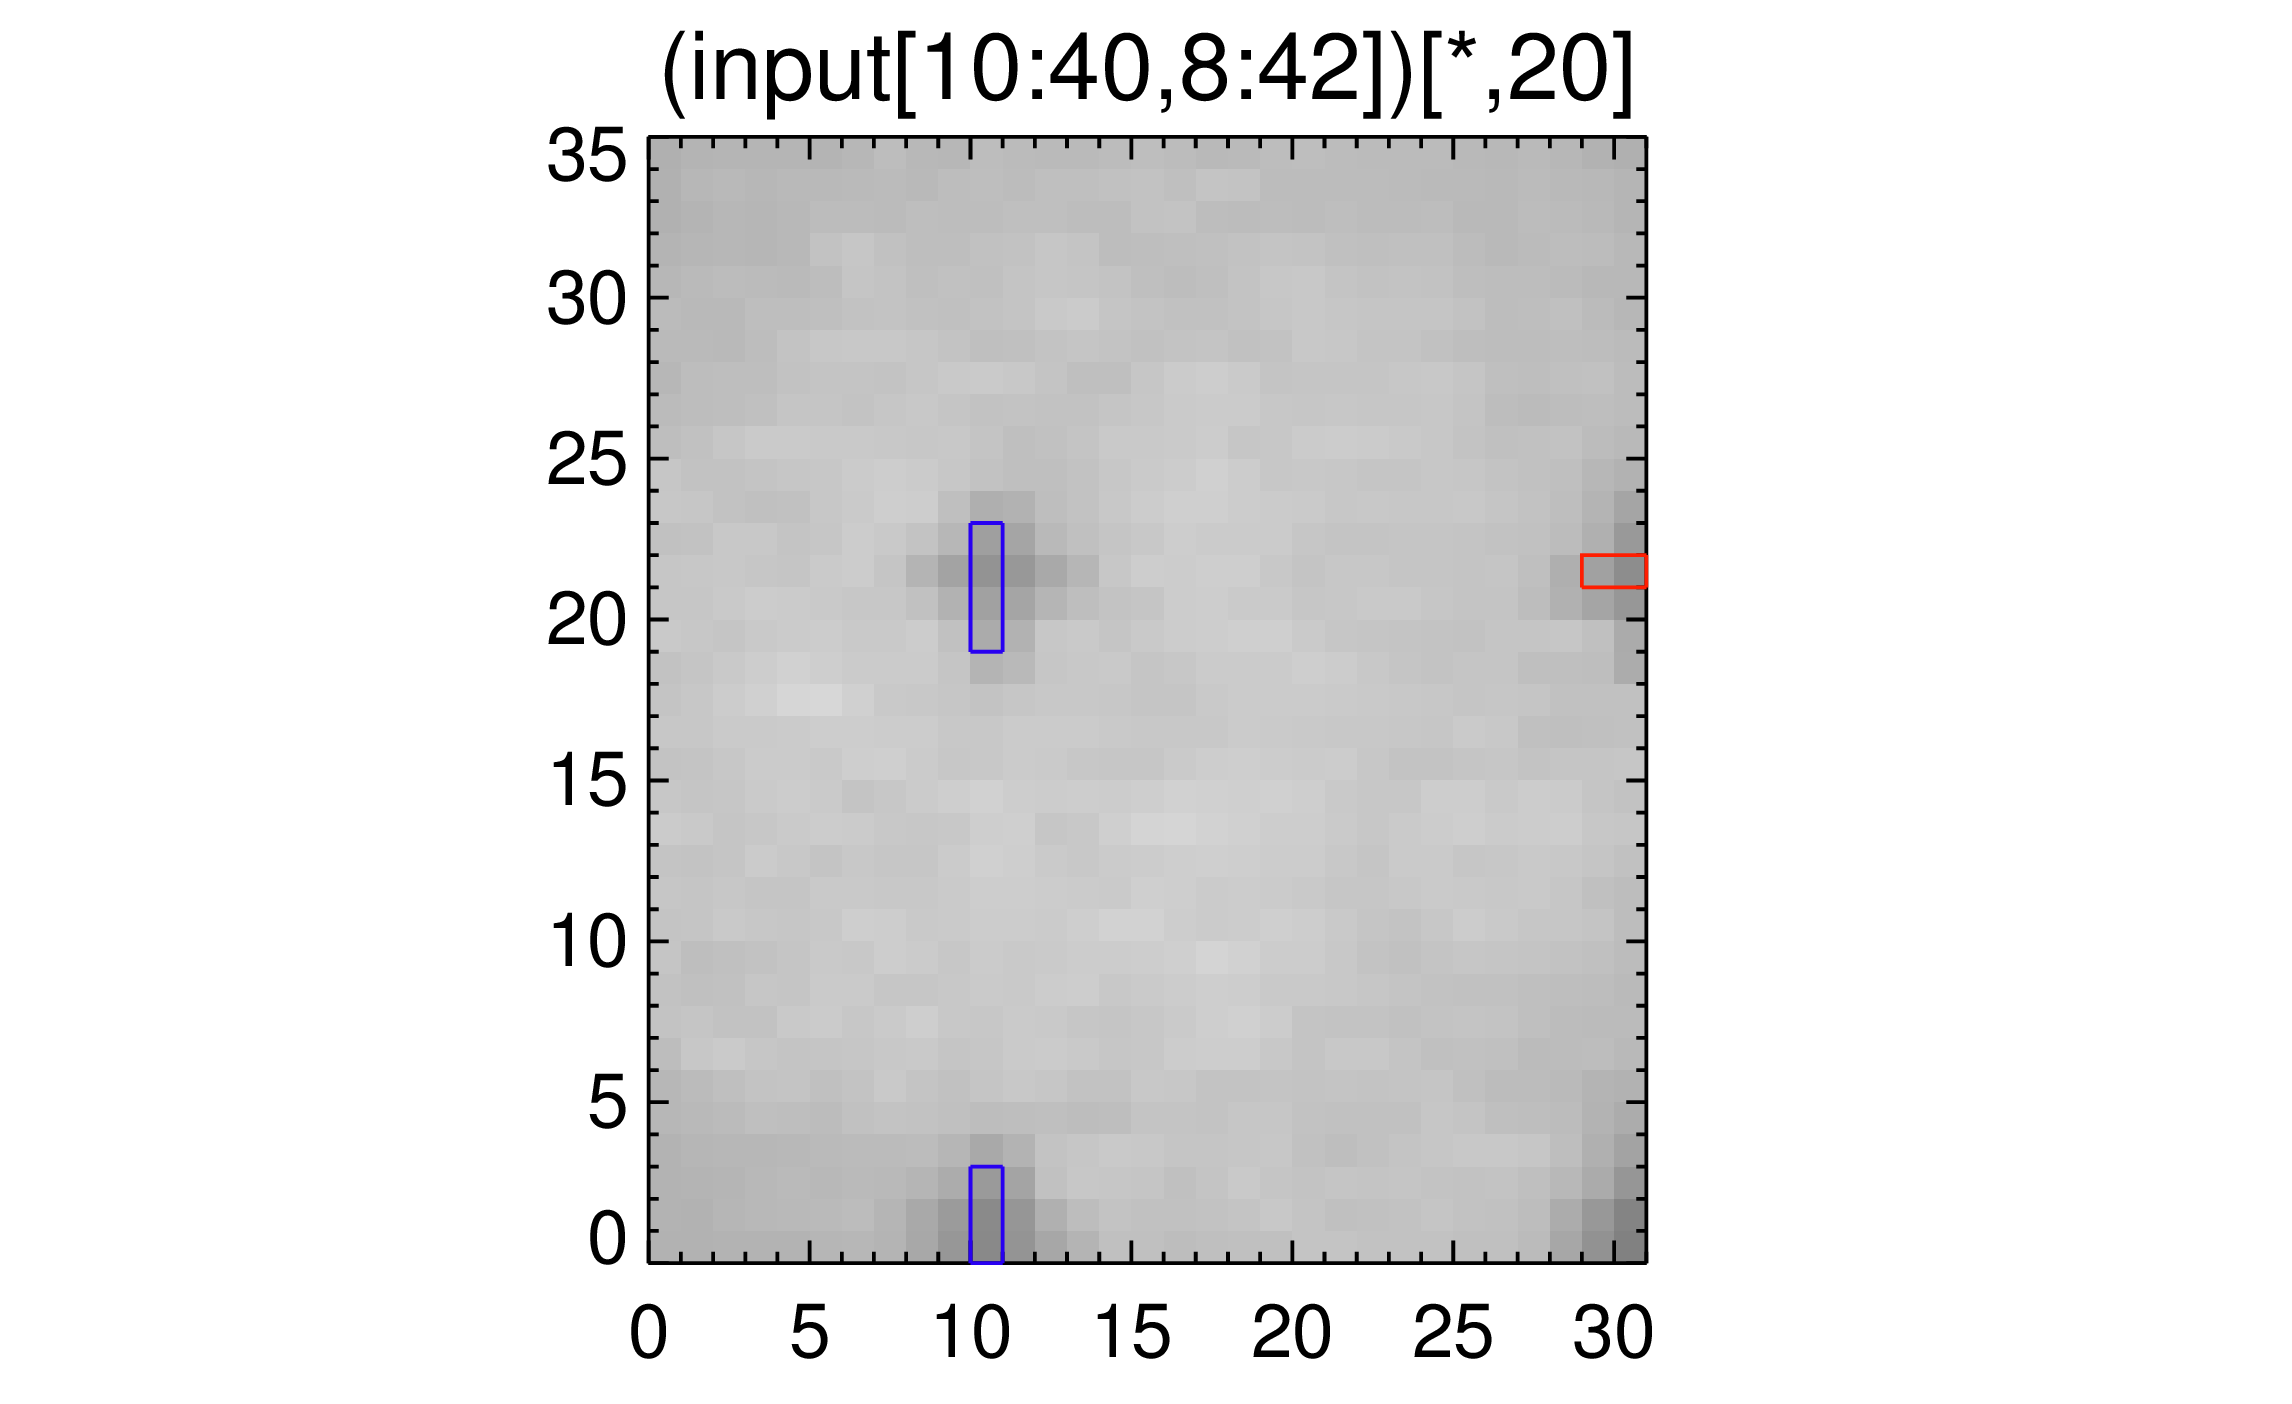
\includegraphics[width=1.3\textwidth]{../plots_tables_images/fidcheck_newdegree2.png}
%         \caption{3 pixels}
%     \end{subfigure}
%     \begin{subfigure}[b]{.45\linewidth}
%         \centering
%         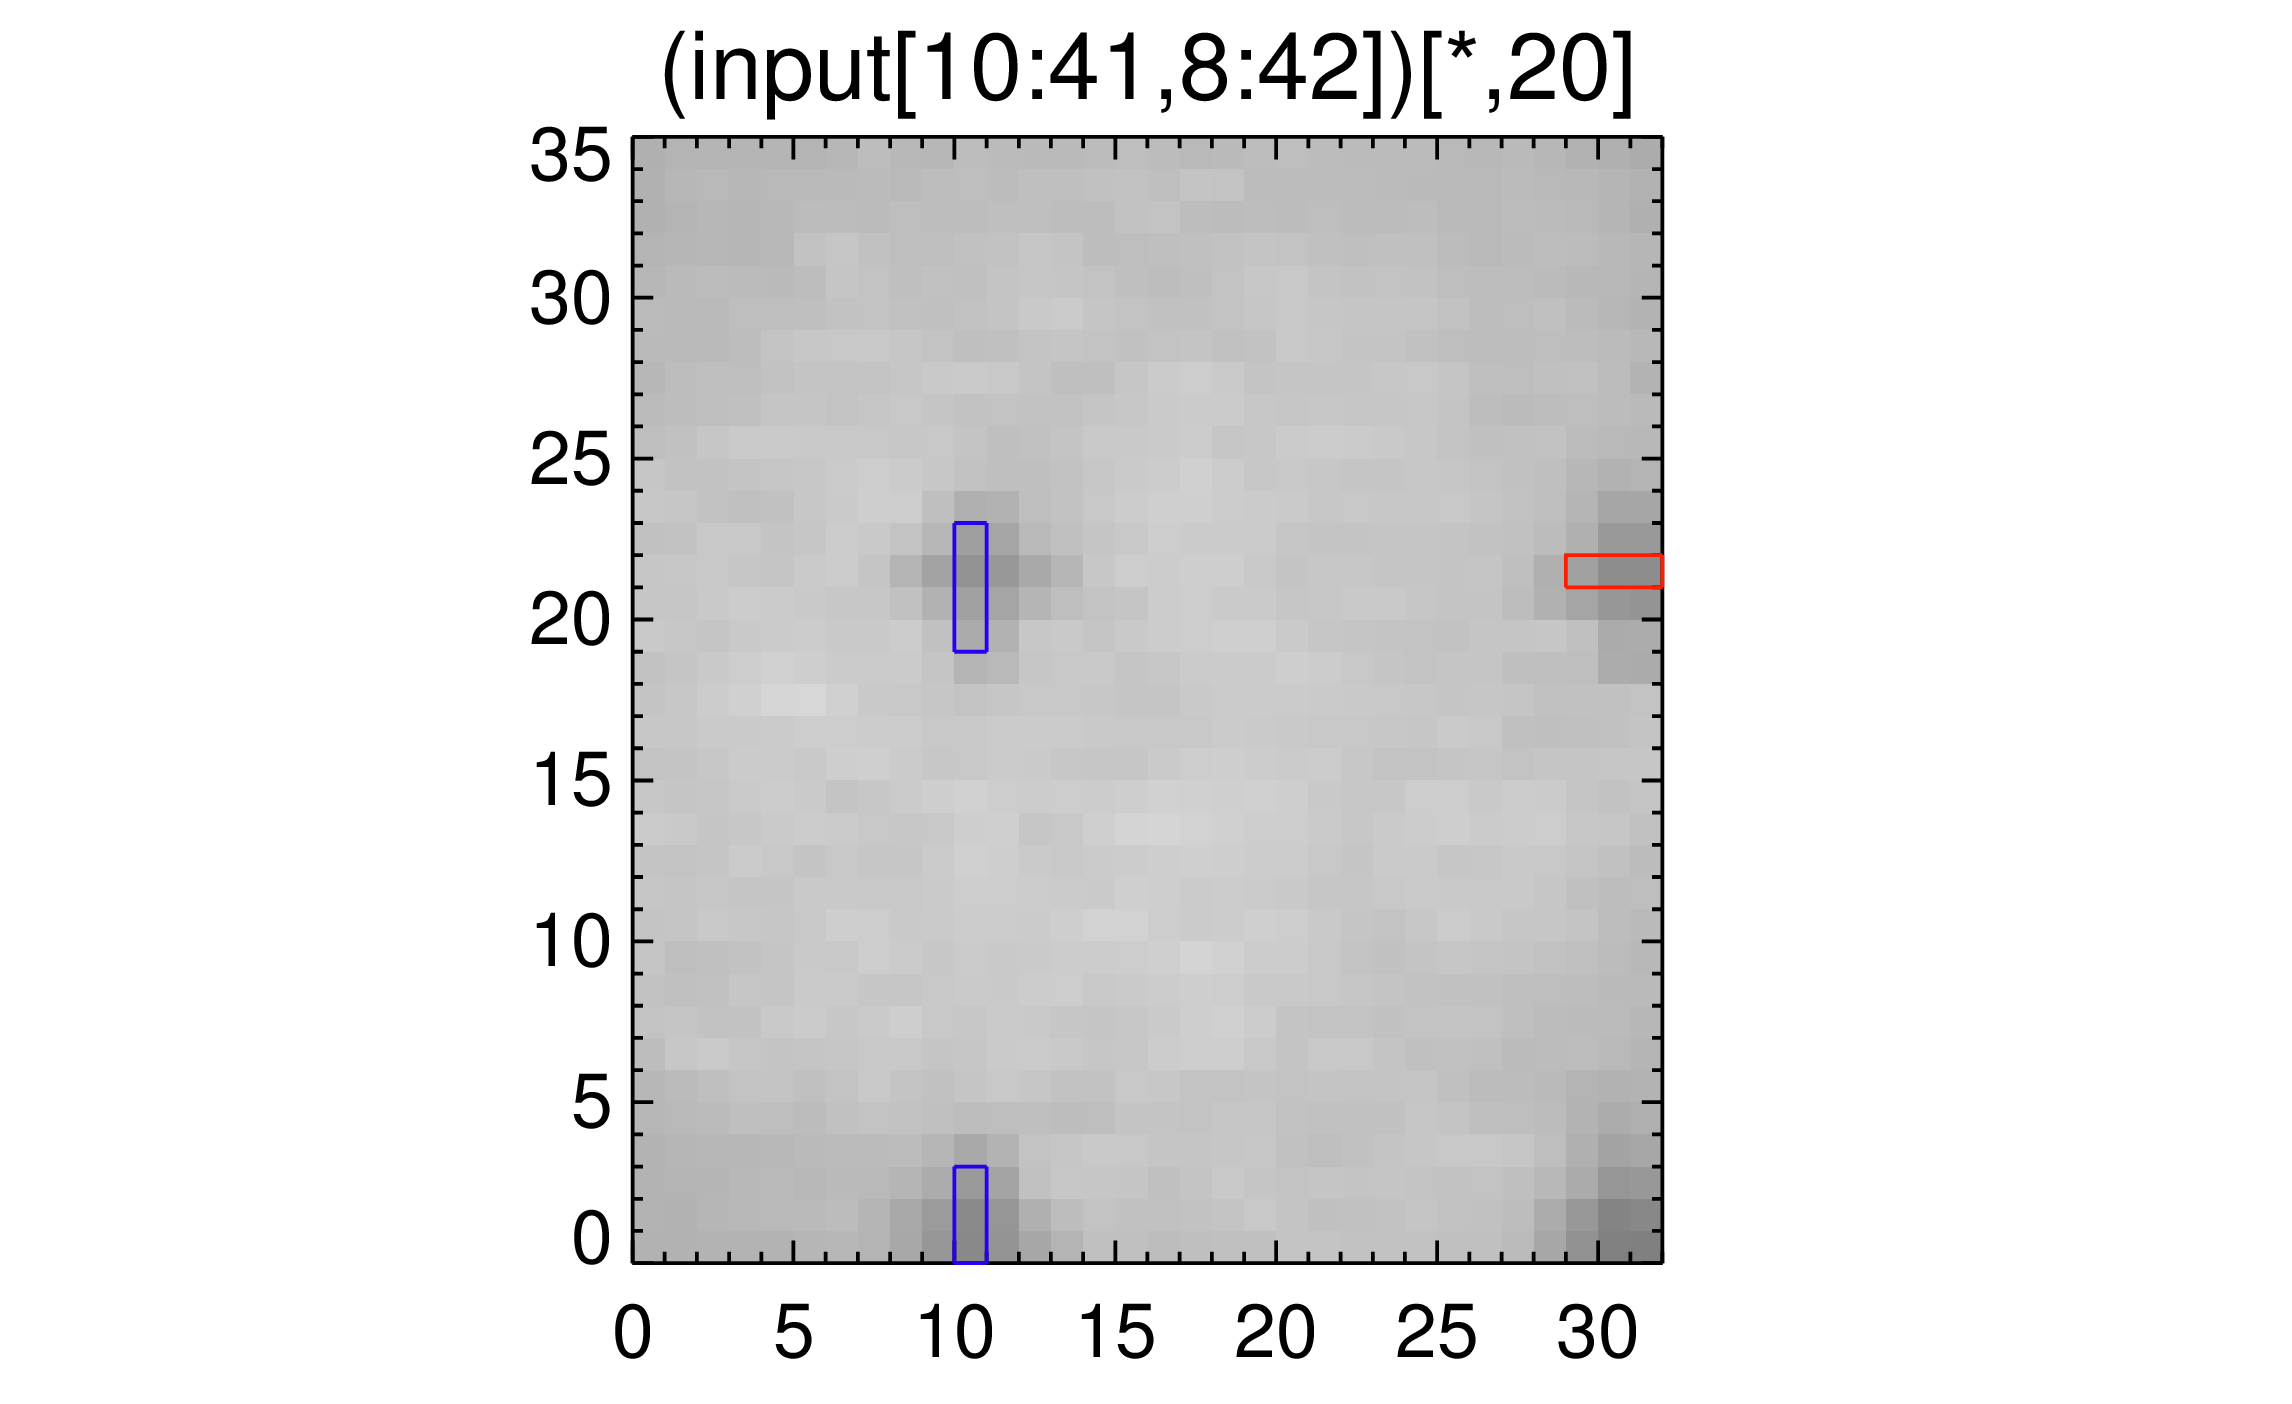
\includegraphics[width=1.3\textwidth]{../plots_tables_images/fidcheck_newdegree3.png}
%         \caption{4 pixels}
%     \end{subfigure}

%     \begin{subfigure}[b]{.45\linewidth}
%         \centering
%         \includegraphics[width=1.3\textwidth]{../plots_tables_images/fidcheck_newdegree4.png}
%         \caption{5 pixels}
%     \end{subfigure}
%     \begin{subfigure}[b]{.45\linewidth}
%         \centering
%         \includegraphics[width=1.3\textwidth]{../plots_tables_images/fidcheck_newdegree5.png}
%         \caption{Completely in image}
%     \end{subfigure}
%     \caption{Finding the left edge of the fiducual now, instead of the right edge of the fiducial}
%     \label{isitok}
% \end{figure}

Compared to Figure \ref{firstplot}, we see that in both instances the fiducials were only detected with 5 pixels in the image, regardless of which side of the fiducial we tried to identify.

% subsection changing_direction_of_edge_filters (end)


% section running_2_edge_detection_filters_on_an_image_with_cut_off_fiducials (end)
\end{document}